% Options for packages loaded elsewhere
\PassOptionsToPackage{unicode}{hyperref}
\PassOptionsToPackage{hyphens}{url}
\PassOptionsToPackage{dvipsnames,svgnames,x11names}{xcolor}
%
\documentclass[
  10pt,
]{article}
\usepackage{amsmath,amssymb}
\usepackage{iftex}
\ifPDFTeX
  \usepackage[T1]{fontenc}
  \usepackage[utf8]{inputenc}
  \usepackage{textcomp} % provide euro and other symbols
\else % if luatex or xetex
  \usepackage{unicode-math} % this also loads fontspec
  \defaultfontfeatures{Scale=MatchLowercase}
  \defaultfontfeatures[\rmfamily]{Ligatures=TeX,Scale=1}
\fi
\usepackage{lmodern}
\ifPDFTeX\else
  % xetex/luatex font selection
  \setmainfont[]{DejaVu Serif}
  \setsansfont[]{DejaVu Sans}
  \setmonofont[]{DejaVu Sans Mono}
  \setmathfont[]{Latin Modern Math}
\fi
% Use upquote if available, for straight quotes in verbatim environments
\IfFileExists{upquote.sty}{\usepackage{upquote}}{}
\IfFileExists{microtype.sty}{% use microtype if available
  \usepackage[]{microtype}
  \UseMicrotypeSet[protrusion]{basicmath} % disable protrusion for tt fonts
}{}
\makeatletter
\@ifundefined{KOMAClassName}{% if non-KOMA class
  \IfFileExists{parskip.sty}{%
    \usepackage{parskip}
  }{% else
    \setlength{\parindent}{0pt}
    \setlength{\parskip}{6pt plus 2pt minus 1pt}}
}{% if KOMA class
  \KOMAoptions{parskip=half}}
\makeatother
\usepackage{xcolor}
\usepackage[margin=2.0cm]{geometry}
\usepackage{color}
\usepackage{fancyvrb}
\newcommand{\VerbBar}{|}
\newcommand{\VERB}{\Verb[commandchars=\\\{\}]}
\DefineVerbatimEnvironment{Highlighting}{Verbatim}{commandchars=\\\{\}}
% Add ',fontsize=\small' for more characters per line
\newenvironment{Shaded}{}{}
\newcommand{\AlertTok}[1]{\textcolor[rgb]{1.00,0.00,0.00}{\textbf{#1}}}
\newcommand{\AnnotationTok}[1]{\textcolor[rgb]{0.38,0.63,0.69}{\textbf{\textit{#1}}}}
\newcommand{\AttributeTok}[1]{\textcolor[rgb]{0.49,0.56,0.16}{#1}}
\newcommand{\BaseNTok}[1]{\textcolor[rgb]{0.25,0.63,0.44}{#1}}
\newcommand{\BuiltInTok}[1]{\textcolor[rgb]{0.00,0.50,0.00}{#1}}
\newcommand{\CharTok}[1]{\textcolor[rgb]{0.25,0.44,0.63}{#1}}
\newcommand{\CommentTok}[1]{\textcolor[rgb]{0.38,0.63,0.69}{\textit{#1}}}
\newcommand{\CommentVarTok}[1]{\textcolor[rgb]{0.38,0.63,0.69}{\textbf{\textit{#1}}}}
\newcommand{\ConstantTok}[1]{\textcolor[rgb]{0.53,0.00,0.00}{#1}}
\newcommand{\ControlFlowTok}[1]{\textcolor[rgb]{0.00,0.44,0.13}{\textbf{#1}}}
\newcommand{\DataTypeTok}[1]{\textcolor[rgb]{0.56,0.13,0.00}{#1}}
\newcommand{\DecValTok}[1]{\textcolor[rgb]{0.25,0.63,0.44}{#1}}
\newcommand{\DocumentationTok}[1]{\textcolor[rgb]{0.73,0.13,0.13}{\textit{#1}}}
\newcommand{\ErrorTok}[1]{\textcolor[rgb]{1.00,0.00,0.00}{\textbf{#1}}}
\newcommand{\ExtensionTok}[1]{#1}
\newcommand{\FloatTok}[1]{\textcolor[rgb]{0.25,0.63,0.44}{#1}}
\newcommand{\FunctionTok}[1]{\textcolor[rgb]{0.02,0.16,0.49}{#1}}
\newcommand{\ImportTok}[1]{\textcolor[rgb]{0.00,0.50,0.00}{\textbf{#1}}}
\newcommand{\InformationTok}[1]{\textcolor[rgb]{0.38,0.63,0.69}{\textbf{\textit{#1}}}}
\newcommand{\KeywordTok}[1]{\textcolor[rgb]{0.00,0.44,0.13}{\textbf{#1}}}
\newcommand{\NormalTok}[1]{#1}
\newcommand{\OperatorTok}[1]{\textcolor[rgb]{0.40,0.40,0.40}{#1}}
\newcommand{\OtherTok}[1]{\textcolor[rgb]{0.00,0.44,0.13}{#1}}
\newcommand{\PreprocessorTok}[1]{\textcolor[rgb]{0.74,0.48,0.00}{#1}}
\newcommand{\RegionMarkerTok}[1]{#1}
\newcommand{\SpecialCharTok}[1]{\textcolor[rgb]{0.25,0.44,0.63}{#1}}
\newcommand{\SpecialStringTok}[1]{\textcolor[rgb]{0.73,0.40,0.53}{#1}}
\newcommand{\StringTok}[1]{\textcolor[rgb]{0.25,0.44,0.63}{#1}}
\newcommand{\VariableTok}[1]{\textcolor[rgb]{0.10,0.09,0.49}{#1}}
\newcommand{\VerbatimStringTok}[1]{\textcolor[rgb]{0.25,0.44,0.63}{#1}}
\newcommand{\WarningTok}[1]{\textcolor[rgb]{0.38,0.63,0.69}{\textbf{\textit{#1}}}}
\usepackage{longtable,booktabs,array}
\usepackage{calc} % for calculating minipage widths
% Correct order of tables after \paragraph or \subparagraph
\usepackage{etoolbox}
\makeatletter
\patchcmd\longtable{\par}{\if@noskipsec\mbox{}\fi\par}{}{}
\makeatother
% Allow footnotes in longtable head/foot
\IfFileExists{footnotehyper.sty}{\usepackage{footnotehyper}}{\usepackage{footnote}}
\makesavenoteenv{longtable}
\usepackage{graphicx}
\makeatletter
\def\maxwidth{\ifdim\Gin@nat@width>\linewidth\linewidth\else\Gin@nat@width\fi}
\def\maxheight{\ifdim\Gin@nat@height>\textheight\textheight\else\Gin@nat@height\fi}
\makeatother
% Scale images if necessary, so that they will not overflow the page
% margins by default, and it is still possible to overwrite the defaults
% using explicit options in \includegraphics[width, height, ...]{}
\setkeys{Gin}{width=\maxwidth,height=\maxheight,keepaspectratio}
% Set default figure placement to htbp
\makeatletter
\def\fps@figure{htbp}
\makeatother
\setlength{\emergencystretch}{3em} % prevent overfull lines
\providecommand{\tightlist}{%
  \setlength{\itemsep}{0pt}\setlength{\parskip}{0pt}}
\setcounter{secnumdepth}{-\maxdimen} % remove section numbering
% doc_header.tex -- LaTeX preamble additions used by build_docs.sh for every
% Markdown -> LaTeX -> PDF conversion (supplements, README, submission files).
\usepackage{etoolbox}
% longtable may not be loaded by pandoc when a document has no table
\usepackage{longtable}
% bold vectors: \bm -> \symbf under unicode-math (XeLaTeX), bm package otherwise
\makeatletter
\@ifpackageloaded{unicode-math}{\providecommand{\bm}[1]{\symbf{#1}}}{\usepackage{bm}}
\makeatother
% smaller type in long tables so that wide audit tables fit the text width;
% inside a table a line break is allowed after an underscore of plain text
% (pandoc writes it as \_), so that long identifiers wrap inside their column
% rows are set a little apart, so that symbols with indices do not touch
\AtBeginEnvironment{longtable}{\footnotesize\renewcommand{\arraystretch}{1.45}%
  \let\sptunderscore\_\def\_{\sptunderscore\allowbreak}}
\setlength{\LTcapwidth}{\textwidth}
% allow line breaks after slashes and hyphens inside table cells
\usepackage{xurl}
% code blocks: break over-long lines instead of running into the margin.
% Plain ``` blocks are typeset by pandoc as {verbatim}, highlighted ones
% (```bash) as {Highlighting}; both are re-declared as breakable fancyvrb
% environments.  The continuation line is marked with a small hooked arrow.
\usepackage{fvextra}
\RecustomVerbatimEnvironment{verbatim}{Verbatim}{breaklines,breakanywhere,fontsize=\small}
\makeatletter
\@ifundefined{Highlighting}{}{%
  \RecustomVerbatimEnvironment{Highlighting}{Verbatim}{breaklines,breakanywhere,fontsize=\small,commandchars=\\\{\}}}
\makeatother
% inline code (pandoc writes it as \texttt{...}): never hyphenate -- an inserted
% hyphen could be read as part of a file name -- but allow a line break after
% an underscore, slash, comma, colon or equals sign, so that long paths and
% column lists wrap inside the text width and inside table columns.
% Inside a formula (e.g. the name of a notebook symbol in an equation) the same
% command must first leave math mode, which \text of amsmath does.
\ExplSyntaxOn
\tl_new:N \l__spt_code_tl
\cs_new_protected:Npn \__spt_texttt:n #1
  {
    \tl_set:Nn \l__spt_code_tl {#1}
    \regex_replace_all:nnN { ([\/\,\:\=]) } { \1 \c{allowbreak} } \l__spt_code_tl
    \regex_replace_all:nnN { \c{_} } { \c{_} \c{allowbreak} } \l__spt_code_tl
    \group_begin: \ttfamily \hyphenchar \font = -1 \scan_stop: \l__spt_code_tl \group_end:
  }
\RenewDocumentCommand \texttt { m }
  {
    \mode_if_math:TF { \text { \__spt_texttt:n {#1} } } { \__spt_texttt:n {#1} }
  }
\ExplSyntaxOff
% A figure is written in the Markdown source as an image paragraph followed by
% a caption paragraph ("**Figure S1.** ..."), so that the caption is also
% visible on GitHub.  An image that starts a paragraph is centered.
\usepackage{graphicx}% pandoc loads it only for documents that contain an image
\NewCommandCopy\sptincludegraphics\includegraphics
\RenewDocumentCommand\includegraphics{O{} m}{%
  \ifvmode\begin{center}\sptincludegraphics[#1]{#2}\end{center}%
  \else\sptincludegraphics[#1]{#2}\fi}
% keep figures where they are referenced
\usepackage{float}
\floatplacement{figure}{H}
% running header with the document title
\usepackage{fancyhdr}
\pagestyle{fancy}
\fancyhf{}
\fancyhead[L]{\small PROJECT spacetimes, Revision\_Deflation\_CJT\_and\_Kohn-Sham\_definition\_C}
\fancyhead[R]{\small\thepage}
\renewcommand{\headrulewidth}{0.4pt}
% 16x16 matrices: tighter columns so that a full matrix fits the text width
\setlength{\arraycolsep}{3.2pt}
% The documents of this project contain long tagged symbols, file paths and
% identifiers that cannot be hyphenated.  A paragraph is therefore allowed to
% have looser lines before TeX gives up and lets a line stick out of the margin.
\AtBeginDocument{\tolerance=2000 \emergencystretch=5em \hbadness=2000}
\ifLuaTeX
  \usepackage{selnolig}  % disable illegal ligatures
\fi
\IfFileExists{bookmark.sty}{\usepackage{bookmark}}{\usepackage{hyperref}}
\IfFileExists{xurl.sty}{\usepackage{xurl}}{} % add URL line breaks if available
\urlstyle{same}
\hypersetup{
  pdftitle={Dirac matrices, Lagrangians and field equations on the deflating 4+4 and 7+1 spacetimes},
  pdfauthor={Patrick Lee Nash, Ph.D.},
  colorlinks=true,
  linkcolor={blue},
  filecolor={Maroon},
  citecolor={blue},
  urlcolor={blue},
  pdfcreator={LaTeX via pandoc}}

\title{Dirac matrices, Lagrangians and field equations on the deflating
4+4 and 7+1 spacetimes}
\usepackage{etoolbox}
\makeatletter
\providecommand{\subtitle}[1]{% add subtitle to \maketitle
  \apptocmd{\@title}{\par {\large #1 \par}}{}{}
}
\makeatother
\subtitle{With mass term and self-interaction. PROJECT spacetimes,
Revision\_Deflation\_CJT\_and\_Kohn-Sham\_definition\_C: definitions,
derivations, exact checks, and how to repeat them}
\author{Patrick Lee Nash, Ph.D.}
\date{November 13, 2026}

\begin{document}
\maketitle

\hypertarget{what-this-document-contains}{%
\section{0. What this document
contains}\label{what-this-document-contains}}

This document defines the 16-component Dirac field on two
eight-dimensional spacetimes whose coordinates \(x5\), \(x6\), \(x7\)
deflate exponentially, and derives its equations. It gives, for each of
the two spacetimes,

\begin{enumerate}
\def\labelenumi{\arabic{enumi}.}
\tightlist
\item
  the metric, its curvature and its symmetries (Part 1);
\item
  the eight real \(16\times16\) Dirac matrices, printed in full, and the
  spin connection (Part 2);
\item
  the Lagrangian with its three parts: the kinetic term, the
  \textbf{mass term} and the \textbf{self-interaction}, which is quartic
  in the field (Part 3);
\item
  the field equation that follows from it, the change of normalization
  that removes the deflation from the equation of fields that do not
  depend on the deflating coordinates, and the conserved current (Part
  4);
\item
  on the 4+4 spacetime, the two forms that the self-interaction can take
  once the theory is quantized: \textbf{form C}, the covariant form,
  which is the definition of the 4+4 model, and \textbf{form Q}, the
  quantized-sector form, which is the alternative; both are written out
  completely, with the exact relation between them (Part 5);
\item
  the algebra of the self-interaction: of its nine couplings only four
  are independent, and uniform matter and a pair of particles feel fixed
  combinations of them, which on 4+4 depend on the form; the
  consequences of the two forms for matter and for the vacuum, in
  numbers; and a discussion of the two forms (Part 6);
\item
  the solutions of the equation without self-interaction, mode by mode
  (Part 7), and the symmetries that survive the deflation (Part 8).
\end{enumerate}

It is written for a reader who knows the Dirac equation of
four-dimensional flat spacetime and the elements of general relativity,
and nothing of this project. Every symbol is defined where it first
appears, and Appendix B lists every symbol of the project with its
meaning. Every equation is derived here or verified here; no other
document is needed to read this one. Statements marked with an
identifier such as \texttt{71d-C3} are verified by a program, exactly
(in integer or rational arithmetic) unless the word ``numerical'' is
used; Appendix A prints the complete output of these programs, and
Section 0.3 says how to run them.

\hypertarget{the-hypotheses}{%
\subsection{0.1 The hypotheses}\label{the-hypotheses}}

The eight coordinates are written \(x0,x1,\dots,x7\), with the digit as
part of the name. \(x1,x2,x3\) are the coordinates of ordinary space and
\(x4\) is the ordinary time. \(x0\) is a fourth, hidden space-like
coordinate. The remaining three, \(x5,x6,x7\), are extra coordinates,
and the two models differ in their character:

\begin{longtable}[]{@{}lll@{}}
\toprule\noalign{}
& 4+4 spacetime & 7+1 spacetime \\
\midrule\noalign{}
\endhead
\bottomrule\noalign{}
\endlastfoot
space-like coordinates & \(x0,x1,x2,x3\) & \(x0,x1,x2,x3,x5,x6,x7\) \\
time-like coordinates & \(x4,x5,x6,x7\) & \(x4\) \\
the Dirac field & \(\psi_{1644d}\) & \(\psi_{1671d}\) \\
\end{longtable}

\textbf{Deflation.} The author's hypothesis is that each of the three
extra coordinates deflates exponentially in the ordinary time: in place
of flat spacetime there is a pseudo-Riemannian space with a diagonal
metric whose components along \(x5,x6,x7\) are

\[\text{4+4:}\quad g^{(4+4)}_{tt}=-\,\mathrm{const}_t^{\,2}\,e^{-2\,\mathrm{rate}_t\,x4},\qquad\qquad
\text{7+1:}\quad g^{(7+1)}_{tt}=+\,\mathrm{const}_t^{\,2}\,e^{-2\,\mathrm{rate}_t\,x4},\qquad t=5,6,7.\tag{0.1}\]

Here \(\mathrm{rate}_5=\mathrm{g55}\), \(\mathrm{rate}_6=\mathrm{g66}\)
and \(\mathrm{rate}_7=\mathrm{g77}\) are three positive constants, the
\textbf{rates of deflation} (the names \(\mathrm{g55}\),
\(\mathrm{g66}\), \(\mathrm{g77}\) are the author's; they are written
upright and never carry a subscript), and \(\mathrm{const}_5\),
\(\mathrm{const}_6\), \(\mathrm{const}_7\) are three positive constants
that may differ from one another and between the two spacetimes. The
superscript \((4+4)\) or \((7+1)\) marks a component of the metric, so
that the component \(g^{(4+4)}_{55}\) cannot be taken for the rate
\(\mathrm{g55}\). The other five diagonal components are those of flat
spacetime.

\textbf{The field.} The field has sixteen complex components. Its
Lagrangian contains a mass term, bilinear in the field, and a
self-interaction, quartic in the field; a theory of a scalar field
\(\phi\) would call them the ``\(\phi^2\)'' and the ``\(\phi^4\)'' term.

\hypertarget{conventions}{%
\subsection{0.2 Conventions}\label{conventions}}

\begin{itemize}
\tightlist
\item
  Units: \(\hbar=c=1\).
\item
  \textbf{Sign of the metric:} space-like components are positive,
  time-like components are negative, as in Eq. (0.1).
\item
  Greek indices \(\mu,\nu,\rho,\sigma,\lambda\) label the coordinates
  and take the values \(0,\dots,7\). Capital indices \(A,B,C\) label the
  directions of an orthonormal frame (Section 1.1) and take the same
  values. The index \(j\) takes the values \(0,1,2,3\) (the flat
  directions), and the indices \(t,s\) take the values \(5,6,7\) (the
  deflating directions).
\item
  Repeated Greek or capital indices, one up and one down, are summed. An
  index \(t\) or \(s\) is summed only where a sum sign says so.
\item
  \(\partial_\mu=\partial/\partial x\mu\); a prime is not used for
  derivatives.
\item
  \(1\) denotes a unit matrix of the size that the context requires,
  \(1_8\) the \(8\times8\) unit matrix; \(M^T\) is the transpose of a
  matrix \(M\), \(M^\dagger\) its Hermitian conjugate, \([M,N]=MN-NM\).
\item
  Where a statement holds on both spacetimes with different signs, the
  sign is written with the constants \(c_\gamma\) and
  \(\mathrm{gs}_{tt}\) of the following table.
\end{itemize}

\begin{longtable}[]{@{}
  >{\raggedright\arraybackslash}p{(\columnwidth - 6\tabcolsep) * \real{0.2500}}
  >{\raggedright\arraybackslash}p{(\columnwidth - 6\tabcolsep) * \real{0.2500}}
  >{\raggedright\arraybackslash}p{(\columnwidth - 6\tabcolsep) * \real{0.2500}}
  >{\raggedright\arraybackslash}p{(\columnwidth - 6\tabcolsep) * \real{0.2500}}@{}}
\toprule\noalign{}
\begin{minipage}[b]{\linewidth}\raggedright
constant
\end{minipage} & \begin{minipage}[b]{\linewidth}\raggedright
meaning
\end{minipage} & \begin{minipage}[b]{\linewidth}\raggedright
4+4
\end{minipage} & \begin{minipage}[b]{\linewidth}\raggedright
7+1
\end{minipage} \\
\midrule\noalign{}
\endhead
\bottomrule\noalign{}
\endlastfoot
\(\mathrm{gs}_{AA}\) & sign of the component \(AA\) of the flat metric &
\(+1\) for \(A=0,1,2,3\); \(-1\) for \(A=4,5,6,7\) & \(-1\) for \(A=4\);
\(+1\) otherwise \\
\(\mathrm{gs}_{tt}\) & that sign for the deflating directions & \(-1\) &
\(+1\) \\
\(c_\gamma\) & sign in the anticommutator of the Dirac matrices, Eq.
(2.1) & \(+1\) & \(-1\) \\
\end{longtable}

On both spacetimes \(c_\gamma\,\mathrm{gs}_{tt}=-1\) and
\(\mathrm{gs}_{44}=-1\); several results below are the same on both for
this reason.

\hypertarget{how-to-repeat-every-result-of-this-document}{%
\subsection{0.3 How to repeat every result of this
document}\label{how-to-repeat-every-result-of-this-document}}

All commands are run from the folder
\texttt{Revision\_Deflation\_CJT\_and\_Kohn-Sham\_definition\_C} of the
repository \texttt{https://github.com/once-ere/spacetimes}. They need a
Rust toolchain (\texttt{cargo}) and Python 3 with the packages numpy,
scipy, sympy, mpmath and matplotlib; the last two lines also need pandoc
and XeLaTeX.

\begin{Shaded}
\begin{Highlighting}[]
\CommentTok{\# 1. compile the program and run its unit tests}
\ExtensionTok{cargo}\NormalTok{ test  }\AttributeTok{{-}{-}release} \AttributeTok{{-}{-}manifest{-}path}\NormalTok{ code/deflation{-}cjt{-}ks{-}c{-}rs/Cargo.toml}
\ExtensionTok{cargo}\NormalTok{ build }\AttributeTok{{-}{-}release} \AttributeTok{{-}{-}manifest{-}path}\NormalTok{ code/deflation{-}cjt{-}ks{-}c{-}rs/Cargo.toml}
\VariableTok{B}\OperatorTok{=}\NormalTok{code/deflation{-}cjt{-}ks{-}c{-}rs/target/release/deflation\_cjt\_ks\_c}

\CommentTok{\# 2. geometry, matrices, spin connection, Dirac operators (Parts 1, 2, 4)}
\VariableTok{$B}\NormalTok{ matrices}
\CommentTok{\# 3. the self{-}interaction (Parts 3, 5, 6); the two forms on 4+4 in numbers (Section 6.6)}
\VariableTok{$B}\NormalTok{ selfcoupling}
\VariableTok{$B}\NormalTok{ forms}
\CommentTok{\# 4. the solutions mode by mode (Part 7) and the symmetries (Part 8)}
\VariableTok{$B}\NormalTok{ modes}
\VariableTok{$B}\NormalTok{ symmetry}
\CommentTok{\# 4a. the stability of the solution of Section 1.4}
\VariableTok{$B}\NormalTok{ gravity}

\CommentTok{\# 5. independent verification with computer algebra and other numerical tools}
\ExtensionTok{python3}\NormalTok{ code/scripts/verify\_deflating\_independent.py}
\ExtensionTok{python3}\NormalTok{ code/scripts/verify\_cjt\_ks\_independent.py}

\CommentTok{\# 6. the figures, and this document (Markdown, LaTeX, PDF)}
\ExtensionTok{python3}\NormalTok{ code/scripts/make\_figures.py}
\ExtensionTok{python3}\NormalTok{ code/scripts/write\_symbol\_registry.py}
\ExtensionTok{python3}\NormalTok{ code/scripts/write\_doc\_tables.py}
\ExtensionTok{python3}\NormalTok{ code/scripts/assemble\_docs.py}
\FunctionTok{bash}\NormalTok{ code/scripts/build\_docs.sh }\StringTok{"dirac matrices deflating.md"}
\end{Highlighting}
\end{Shaded}

What each step does. Step 1 compiles the program
\texttt{deflation\_cjt\_ks\_c} (written in Rust) and runs its unit
tests, which must end with \texttt{test\ result:\ ok}; the third line
abbreviates the path of the program. Each command of steps 2 to 4
computes, writes its data files into the folder \texttt{data}, and ends
with a line that counts its checks, for example
\texttt{forms:\ 9\ of\ 9\ checks\ passed}; the complete reports are the
files \texttt{data/deflating\_checks.txt},
\texttt{data/flat\_matrix\_checks.txt},
\texttt{data/selfcoupling\_checks.txt}, \texttt{data/forms\_checks.txt},
\texttt{data/mode\_checks.txt}, \texttt{data/symmetry\_checks.txt} and
\texttt{data/gravity\_checks.txt}, printed in Appendix A. (The command
\texttt{forms} takes about ten minutes; the others take seconds to about
a minute.) Step 5 repeats the central results with other tools (computer
algebra for the geometry and for the algebra of the self-interaction, a
general-purpose integrator and another library of special functions for
the modes). Step 6 draws the figures from the data files and builds this
document; the tables, the printed matrices and the program outputs in it
are inserted by the scripts, not typed.

The source files in which each calculation is written:
\texttt{metric.rs}, \texttt{geometry.rs}, \texttt{curved.rs} (geometry,
spin connection, Dirac operators); \texttt{selfint.rs},
\texttt{cmd\_selfcoupling.rs} (self-interaction); \texttt{halves.rs},
\texttt{cmd\_forms.rs}, \texttt{cmd\_forms\_b.rs} (the two forms on 4+4:
matter of two halves, vacuum); \texttt{modes.rs} (solutions);
\texttt{symmetry\_defl.rs}, \texttt{cmd\_symmetry.rs} (symmetries); all
in \texttt{code/deflation-cjt-ks-c-rs/src/}. Each file begins with a
description of what it computes and how.

\begin{center}\rule{0.5\linewidth}{0.5pt}\end{center}

\hypertarget{part-1.-geometry-of-the-deflating-spacetimes}{%
\section{Part 1. Geometry of the deflating
spacetimes}\label{part-1.-geometry-of-the-deflating-spacetimes}}

\hypertarget{metric-orthonormal-frame-volume}{%
\subsection{1.1 Metric, orthonormal frame,
volume}\label{metric-orthonormal-frame-volume}}

The flat metrics of the two spacetimes are, in the coordinates
\(x0,\dots,x7\),

\[\begin{aligned}
\eta^{(4+4)}&=\mathrm{diag}(+1,+1,+1,+1,-1,-1,-1,-1),\\
\eta^{(7+1)}&=\mathrm{diag}(+1,+1,+1,+1,-1,+1,+1,+1).
\end{aligned}\tag{1.1}\]

Their diagonal entries are the signs \(\mathrm{gs}_{AA}\) of Section
0.2. Define three \textbf{scale factors}, one for each deflating
coordinate,

\[b_t(x4)=\mathrm{const}_t\,e^{-\mathrm{rate}_t\,x4},\qquad t=5,6,7.\tag{1.2}\]

The metric of the deflating spacetime is diagonal:

\[\begin{aligned}
g^{(4+4)}_{\mu\nu}&=\mathrm{diag}\big(+1,+1,+1,+1,-1,-b_5^2,-b_6^2,-b_7^2\big),\\
g^{(7+1)}_{\mu\nu}&=\mathrm{diag}\big(+1,+1,+1,+1,-1,+b_5^2,+b_6^2,+b_7^2\big).
\end{aligned}\tag{1.3}\]

Its last three components are those of the hypothesis (0.1) (checks
\texttt{44d-G1}, \texttt{71d-G1}). In one formula for both spacetimes,
\(g_{tt}=\mathrm{gs}_{tt}\,b_t^2\). A coordinate interval \(dxt\) has
the proper extent \(b_t\,|dxt|\), which shrinks by the factor \(e\) in
the time \(1/\mathrm{rate}_t\): this is the meaning of ``the coordinate
\(xt\) deflates''. On the 7+1 spacetime, where \(x5,x6,x7\) are
space-like, what shrinks is a length; on the 4+4 spacetime, where they
are time-like, it is a duration measured along an additional time. The
inverse metric is written \(g_{(4+4)}^{\mu\nu}\),
\(g_{(7+1)}^{\mu\nu}\); its components along the deflating coordinates
are \(\mathrm{gs}_{tt}/b_t^2\).

\textbf{Frame.} At each point choose eight vector fields
\(e_A=e_A{}^\mu\,\partial_\mu\) that are orthonormal,
\(g_{\mu\nu}\,e_A{}^\mu e_B{}^\nu=\eta_{AB}\). We take them along the
coordinates:

\[e_A{}^\mu=\mathrm{diag}\Big(1,1,1,1,1,\frac1{b_5},\frac1{b_6},\frac1{b_7}\Big),\qquad
e^A{}_\mu=\mathrm{diag}\big(1,1,1,1,1,b_5,b_6,b_7\big),\tag{1.4}\]

where \(e^A{}_\mu\) is the inverse matrix. Frame indices are raised and
lowered with the flat metric (1.1), coordinate indices with the metric
(1.3).

\textbf{Volume.} The invariant volume element is \(V_d\,d^8x\) with

\[V_d(x4)=\sqrt{|\det g|}=b_5\,b_6\,b_7\ \propto\ e^{-\mathrm{gsum}\,x4},\qquad
\mathrm{gsum}=\mathrm{g55}+\mathrm{g66}+\mathrm{g77}.\tag{1.5}\]

\(V_d\) is the proper volume of a unit coordinate cell of the three
deflating coordinates, and the \textbf{total rate} \(\mathrm{gsum}\) is
the rate at which it shrinks. Two further combinations of the rates
occur:

\[\mathrm{gsq}=\mathrm{g55}^2+\mathrm{g66}^2+\mathrm{g77}^2,\qquad
\mathrm{gprod}=\mathrm{g55}\,\mathrm{g66}+\mathrm{g55}\,\mathrm{g77}+\mathrm{g66}\,\mathrm{g77},\qquad
\mathrm{gsum}^2=\mathrm{gsq}+2\,\mathrm{gprod}.\tag{1.6}\]

\hypertarget{christoffel-symbols}{%
\subsection{1.2 Christoffel symbols}\label{christoffel-symbols}}

The Christoffel symbols are
\(\Gamma^\rho{}_{\mu\nu}=\tfrac12\,g^{\rho\sigma}\big(\partial_\mu g_{\sigma\nu}+\partial_\nu g_{\sigma\mu}-\partial_\sigma g_{\mu\nu}\big)\).
The only components of the metric that depend on a coordinate are the
three \(g_{tt}\), and they depend on \(x4\) alone, with
\(\partial_4 g_{tt}=-2\,\mathrm{rate}_t\,g_{tt}\). A Christoffel symbol
therefore differs from zero only if it contains the index pair \(tt\)
and the index 4. With the components \(g_{tt}\) and \(g^{tt}=1/g_{tt}\)
of the metric (1.3) of either spacetime,
\[\Gamma^t{}_{4t}=\Gamma^t{}_{t4}=\tfrac12\,g^{tt}\,\partial_4g_{tt}=-\,\mathrm{rate}_t,\qquad
\Gamma^4{}_{tt}=-\tfrac12\,g^{44}\,\partial_4g_{tt}=-\,\mathrm{gs}_{tt}\,\mathrm{rate}_t\,b_t^2,\tag{1.7}\]

without summation over \(t\), where \(g^{44}=-1\) was used. Thus
\(\Gamma^4{}_{tt}=+\mathrm{rate}_t\,b_t^2\) on the 4+4 spacetime and
\(-\mathrm{rate}_t\,b_t^2\) on the 7+1 spacetime; all other symbols
vanish (checks \texttt{44d-G2}, \texttt{71d-G2}).

\hypertarget{curvature}{%
\subsection{1.3 Curvature}\label{curvature}}

\textbf{Riemann tensor.} With the convention
\(R^\rho{}_{\sigma\mu\nu}=\partial_\mu\Gamma^\rho{}_{\nu\sigma}-\partial_\nu\Gamma^\rho{}_{\mu\sigma}+\Gamma^\rho{}_{\mu\lambda}\Gamma^\lambda{}_{\nu\sigma}-\Gamma^\rho{}_{\nu\lambda}\Gamma^\lambda{}_{\mu\sigma}\)
the components in the orthonormal frame that do not vanish are

\[R^t{}_{4t4}=-\,\mathrm{rate}_t^{\,2},\qquad R^4{}_{t4t}=\mathrm{gs}_{tt}\,\mathrm{rate}_t^{\,2},\qquad
R^t{}_{sts}=\mathrm{gs}_{ss}\,\mathrm{rate}_t\,\mathrm{rate}_s\quad(t\neq s),\tag{1.8}\]

and those that follow from the antisymmetry in the last two indices
(checks \texttt{44d-G4}, \texttt{71d-G4}). No component carries an index
\(0,1,2,3\): \emph{the four coordinates \(x0,x1,x2,x3\) span a flat
space, and the curvature lives in the four coordinates \(x4,x5,x6,x7\).}
The program obtains the curvature in two independent ways, from the
Christoffel symbols and from Cartan's structure equations for the frame
(checks \texttt{44d-G3}, \texttt{71d-G3}).

\textbf{Sectional curvatures.} For a pair of frame directions
\(A\neq B\) the number \(K_{AB}=K_{BA}=R^{AB}{}_{AB}\) (first index
raised with the flat metric, no summation) is the sectional curvature of
the plane that the two directions span. From Eq. (1.8), on both
spacetimes,

\[K_{4t}=\mathrm{rate}_t^{\,2},\qquad K_{ts}=\mathrm{rate}_t\,\mathrm{rate}_s\quad(t\neq s),\qquad
K_{AB}=0\ \text{if}\ A\ \text{or}\ B\in\{0,1,2,3\}.\tag{1.9}\]

(For example
\(K_{4t}=R^{4t}{}_{4t}=\mathrm{gs}_{tt}\,R^4{}_{t4t}=\mathrm{gs}_{tt}^2\,\mathrm{rate}_t^{\,2}\).)
The Riemann tensor of this metric has no other components: it is
``diagonal on pairs of directions''.

\textbf{Ricci tensor, curvature scalar, Einstein tensor.} For such a
Riemann tensor the mixed components of the Ricci tensor are
\(R^A{}_A=\sum_{B\neq A}K_{AB}\), the curvature scalar is
\(R=\sum_{A\neq B}K_{AB}\) (each pair counted twice), and the Einstein
tensor \(\mathcal G^\mu{}_\nu=R^\mu{}_\nu-\tfrac12R\,\delta^\mu_\nu\) is
diagonal with \(\mathcal G^A{}_A=-\sum K_{BC}\), the sum running over
the pairs \(\{B,C\}\) of directions that do not contain \(A\). With Eq.
(1.9):

\[R^4{}_4=\mathrm{gsq},\qquad R^t{}_t=\mathrm{rate}_t\,\mathrm{gsum},\qquad R^j{}_j=0,\qquad
R=\mathrm{gsq}+\mathrm{gsum}^2,\tag{1.10}\]

\[\mathcal G^4{}_4=-\,\mathrm{gprod},\qquad
\mathcal G^j{}_j=-\tfrac12\big(\mathrm{gsq}+\mathrm{gsum}^2\big),\qquad
\mathcal G^t{}_t=\mathrm{rate}_t\,\mathrm{gsum}-\tfrac12\big(\mathrm{gsq}+\mathrm{gsum}^2\big),\tag{1.11}\]

the same on both spacetimes in the sign convention of this document
(checks \texttt{44d-G5}, \texttt{71d-G5}). All are constants: the
curvature does not depend on the time.

\hypertarget{the-deflating-spacetimes-are-not-solutions-of-einsteins-equations-without-matter}{%
\subsection{1.4 The deflating spacetimes are not solutions of Einstein's
equations without
matter}\label{the-deflating-spacetimes-are-not-solutions-of-einsteins-equations-without-matter}}

The Einstein tensor (1.11) does not vanish, and it is not a multiple of
the unit matrix unless all rates vanish: \emph{the deflating spacetime
is not a solution of Einstein's equations without matter, with or
without a cosmological constant.} Something must sustain the deflation.

In more than four dimensions the general field equations of second order
for the metric are those of Lovelock. Their first term beyond Einstein's
is the Lanczos tensor \(\mathcal H^\mu{}_\nu\) of the Gauss--Bonnet
term, and the equations without matter read

\[\mathcal G^\mu{}_\nu+\Lambda_8\,\delta^\mu_\nu+\alpha_{\rm GB}\,\mathcal H^\mu{}_\nu=0\tag{1.12}\]

with a cosmological constant \(\Lambda_8\) and a coupling
\(\alpha_{\rm GB}\). For a Riemann tensor that is diagonal on pairs of
directions, \(\mathcal H^A{}_A=-4\sum K_{BC}\,K_{B'C'}\), where the sum
runs over the unordered couples of two pairs \(\{B,C\}\), \(\{B',C'\}\)
that have no direction in common and do not contain \(A\). A couple
contributes only if its four directions are \(4,5,6,7\), so that

\[\mathcal H^j{}_j=-4\,\big(K_{45}K_{67}+K_{46}K_{57}+K_{47}K_{56}\big)
=-4\,\mathrm{g55}\,\mathrm{g66}\,\mathrm{g77}\,\mathrm{gsum},\qquad
\mathcal H^4{}_4=\mathcal H^t{}_t=0.\tag{1.13}\]

The components of Eq. (1.12) along \(x4,\dots,x7\) contain no
Gauss--Bonnet term and require
\(\mathcal G^4{}_4=\mathcal G^5{}_5=\mathcal G^6{}_6=\mathcal G^7{}_7\);
since
\(\mathcal G^5{}_5-\mathcal G^6{}_6=(\mathrm{g55}-\mathrm{g66})\,\mathrm{gsum}\),
this holds if and only if the three rates are equal. The components
along \(x0,\dots,x3\) then fix the coupling:

\[\mathrm{g55}=\mathrm{g66}=\mathrm{g77}:\qquad\Lambda_8=3\,\mathrm{g55}^2,\qquad
\alpha_{\rm GB}=-\frac{1}{4\,\mathrm{g55}^2}.\tag{1.14}\]

\emph{With three equal rates the deflating spacetime is an exact
solution of Einstein--Gauss--Bonnet gravity without matter; with unequal
rates it is not, for any \(\Lambda_8\) and \(\alpha_{\rm GB}\)} (checks
\texttt{44d-G10}, \texttt{71d-G10}; an independent script obtains the
same Lanczos tensor from its definition by computer algebra). This
solution is not stable. When the common rate of expansion of the four
flat directions and the common rate of the three deflating directions
are allowed to vary, the constraint among the initial data admits, near
the solution, no deflation slower than \(\mathrm{g55}\); and for every
perturbation that it does admit, with or without matter, the deflation
departs from the exponential law and becomes faster and faster (check
\texttt{gr-G5} of the command \texttt{gravity}, numerical; Appendix A.7
prints the report). What sustains the deflation is therefore an open
question of the hypothesis, not answered by this document.

\hypertarget{symmetries}{%
\subsection{1.5 Symmetries}\label{symmetries}}

A \textbf{Killing vector} is a vector field along which the metric does
not change. Flat spacetime in eight dimensions has 36: eight
translations and 28 rotations and boosts, one for each pair of
coordinates. The deflating spacetime has, for any rates, 14:

\begin{itemize}
\tightlist
\item
  the seven translations along all coordinates but \(x4\);
\item
  the six rotations of \(x0,x1,x2,x3\);
\item
  the \textbf{scaling}
  \[\mathcal X_{\rm scale}=\partial_4+\mathrm{g55}\,x5\,\partial_5+\mathrm{g66}\,x6\,\partial_6+\mathrm{g77}\,x7\,\partial_7,\tag{1.15}\]
  which shifts the time and stretches the deflating coordinates so as to
  undo the shrinking.
\end{itemize}

Two equal rates add one Killing vector, the rotation of the two
coordinates concerned (for \(\mathrm{g55}=\mathrm{g66}\) it is
\(\mathrm{const}_6^{\,2}\,x6\,\partial_5-\mathrm{const}_5^{\,2}\,x5\,\partial_6\),
which contains the two constants). Three equal rates add the three
rotations of \(x5,x6,x7\) and three further vectors (Section 1.6), 20 in
all (checks \texttt{44d-G6}, \texttt{71d-G6}). The following table
counts, for three sets of rates, how many of the 28 rotations and boosts
remain symmetries, and how many of six particular rotations, those of
the four axes \(x0,x5,x6,x7\), which Part 8 uses.

\begin{longtable}[]{@{}
  >{\raggedright\arraybackslash}p{(\columnwidth - 16\tabcolsep) * \real{0.1111}}
  >{\raggedleft\arraybackslash}p{(\columnwidth - 16\tabcolsep) * \real{0.1111}}
  >{\raggedleft\arraybackslash}p{(\columnwidth - 16\tabcolsep) * \real{0.1111}}
  >{\raggedleft\arraybackslash}p{(\columnwidth - 16\tabcolsep) * \real{0.1111}}
  >{\raggedleft\arraybackslash}p{(\columnwidth - 16\tabcolsep) * \real{0.1111}}
  >{\raggedleft\arraybackslash}p{(\columnwidth - 16\tabcolsep) * \real{0.1111}}
  >{\raggedleft\arraybackslash}p{(\columnwidth - 16\tabcolsep) * \real{0.1111}}
  >{\raggedleft\arraybackslash}p{(\columnwidth - 16\tabcolsep) * \real{0.1111}}
  >{\raggedleft\arraybackslash}p{(\columnwidth - 16\tabcolsep) * \real{0.1111}}@{}}
\toprule\noalign{}
\begin{minipage}[b]{\linewidth}\raggedright
spacetime
\end{minipage} & \begin{minipage}[b]{\linewidth}\raggedleft
rotations and boosts
\end{minipage} & \begin{minipage}[b]{\linewidth}\raggedleft
isometries, rates (1, 2, 3)
\end{minipage} & \begin{minipage}[b]{\linewidth}\raggedleft
rates (2, 2, 5)
\end{minipage} & \begin{minipage}[b]{\linewidth}\raggedleft
rates (1, 1, 1)
\end{minipage} & \begin{minipage}[b]{\linewidth}\raggedleft
internal generators
\end{minipage} & \begin{minipage}[b]{\linewidth}\raggedleft
of these isometries: (1, 2, 3)
\end{minipage} & \begin{minipage}[b]{\linewidth}\raggedleft
(2, 2, 5)
\end{minipage} & \begin{minipage}[b]{\linewidth}\raggedleft
(1, 1, 1)
\end{minipage} \\
\midrule\noalign{}
\endhead
\bottomrule\noalign{}
\endlastfoot
7+1 & 28 & 6 & 7 & 9 & 6 & 0 & 1 & 3 \\
4+4 & 28 & 6 & 7 & 9 & 6 & 0 & 1 & 3 \\
\end{longtable}

Three consequences. The spacetime is homogeneous: no place and no moment
is distinguished. The constants \(\mathrm{const}_t\) are not observable
by themselves, since a rescaling of \(xt\) changes them. And there is no
conserved energy, because a translation in time alone is not a symmetry.
Nothing that involves the time survives among the rotations and boosts,
in particular not the boosts of special relativity: the deflation
defines a preferred state of rest, as the expansion of the universe
does.

\begin{figure}
\centering
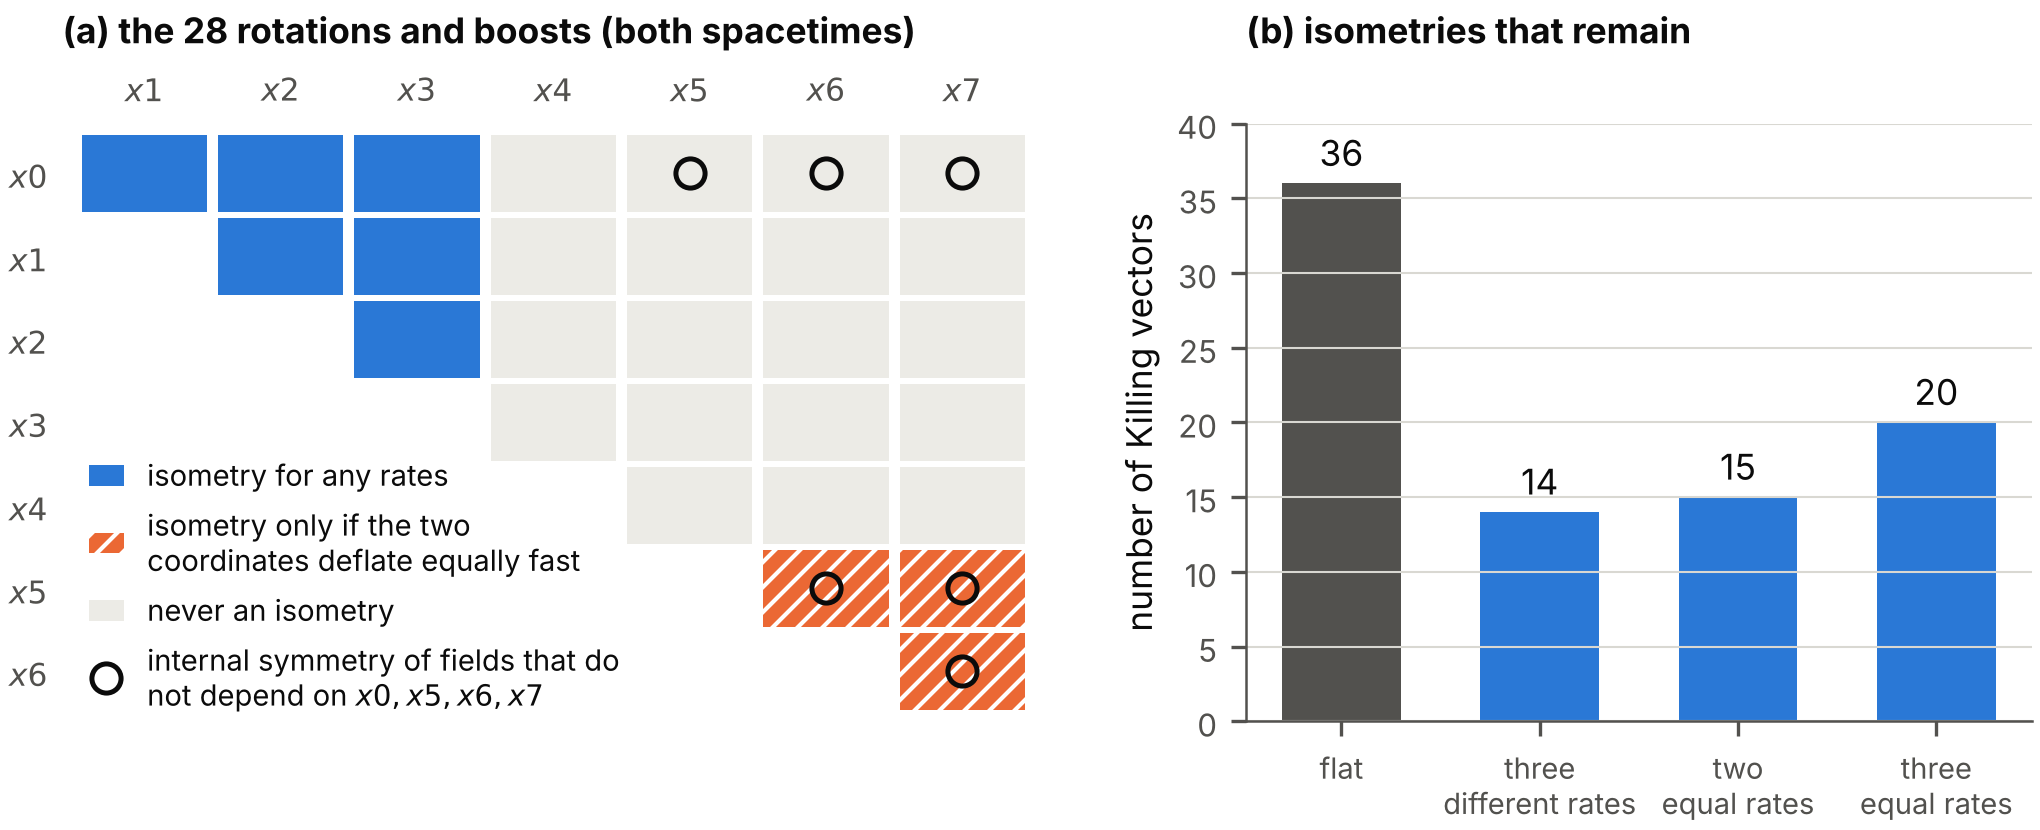
\includegraphics[width=0.92\textwidth,height=\textheight]{figures/fig_isometries.png}
\caption{Symmetries of the deflating spacetimes. (a) The 28 rotations
and boosts of flat spacetime, one square for each pair of coordinates:
those that remain symmetries for any rates, those that remain symmetries
only if the two coordinates deflate equally fast, and those that are
never symmetries. Circles mark the six pairs taken from the axes
\(x0,x5,x6,x7\). (b) The number of Killing vectors.}
\end{figure}

\hypertarget{equal-rates-a-space-of-constant-curvature}{%
\subsection{1.6 Equal rates: a space of constant
curvature}\label{equal-rates-a-space-of-constant-curvature}}

Let \(\mathrm{g55}=\mathrm{g66}=\mathrm{g77}\). Then all sectional
curvatures (1.9) of the four directions \(4,5,6,7\) are equal to
\(\mathrm{g55}^2\): the four coordinates \(x4,\dots,x7\) span a space of
constant curvature. With the new coordinates
\(\bar x4=e^{\mathrm{g55}\,x4}/\mathrm{g55}\) and
\(\bar xt=\mathrm{const}_t\,xt\) the part of the line element that
contains them becomes

\[-dx4^2+\mathrm{gs}_{tt}\,e^{-2\,\mathrm{g55}\,x4}\sum_t d\bar xt^2
=\frac{-d\bar x4^2+\mathrm{gs}_{tt}\sum_t d\bar xt^2}{(\mathrm{g55}\,\bar x4)^2}.\tag{1.16}\]

On the 7+1 spacetime (\(\mathrm{gs}_{tt}=+1\)) this is de Sitter space
of the radius \(1/\mathrm{g55}\) in the half of its flat slicing in
which space contracts. On the 4+4 spacetime (\(\mathrm{gs}_{tt}=-1\)) it
is minus the line element of four-dimensional hyperbolic space of that
radius (checks \texttt{44d-G7}, \texttt{71d-G7}). The line element
(1.16) is a multiple of a flat one, and the special conformal
transformations of that flat metric along the three axes \(\bar xs\)
(\(s=5,6,7\)) are the three further Killing vectors:

\[\mathcal X_{(s)}=2\,\bar xs\,\Big[\bar x4\,\frac{\partial}{\partial\bar x4}+\sum_t\bar xt\,\frac{\partial}{\partial\bar xt}\Big]
-\Big(\sum_t\bar xt^2-\mathrm{gs}_{tt}\,\bar x4^2\Big)\frac{\partial}{\partial\bar xs},\tag{1.17}\]

with
\(\bar x4\,\partial/\partial\bar x4=\mathrm{g55}^{-1}\,\partial_4\).

\hypertarget{geodesics-what-a-classical-particle-does}{%
\subsection{1.7 Geodesics: what a classical particle
does}\label{geodesics-what-a-classical-particle-does}}

The seven translations give seven conserved momenta \(P_\mu\)
(\(\mu\neq4\)) of a classical particle of mass \(m\). Let
\(E_\perp=(m^2+\sum_jP_j^2)^{1/2}\) be the energy that the particle
would have without momentum along the deflating coordinates. The
conservation of the norm of the momentum,
\(g^{\mu\nu}P_\mu P_\nu=-m^2\), gives the velocity along the time, with
an affine parameter \(\varsigma\) along the path:

\[\Big(\frac{dx4}{d\varsigma}\Big)^2=E_\perp^2+\mathrm{gs}_{tt}\sum_t\frac{P_t^2}{b_t(x4)^2}.\tag{1.18}\]

The last term grows as \(e^{2\,\mathrm{rate}_t\,x4}\): the momentum
\(P_t\) belongs to a fixed coordinate wavelength, and the proper
wavelength shrinks.

\emph{7+1} (\(\mathrm{gs}_{tt}=+1\)). The energy of a particle that
moves along a deflating coordinate grows without bound, the reverse of
the redshift in an expanding universe. For momentum along \(x5\) alone
the proper time that elapses between \(x4\) and \(x4=\infty\) is finite,
\(\dfrac{m}{\mathrm{g55}\,E_\perp}\,\mathrm{arsinh}\Big(\dfrac{E_\perp\,\mathrm{const}_5\,e^{-\mathrm{g55}\,x4}}{|P_5|}\Big)\):
the coordinates of Eq. (1.3) do not cover the whole future of such a
particle (check \texttt{71d-G8}, numerical).

\emph{4+4} (\(\mathrm{gs}_{tt}=-1\)). The right-hand side of Eq. (1.18)
vanishes at a \textbf{turning value} of the time; for momentum along
\(x5\) alone,

\[x4_{\rm turn}=\frac{1}{\mathrm{g55}}\,\ln\frac{E_\perp\,\mathrm{const}_5}{|P_5|}.\tag{1.19}\]

The path reaches this value and returns to smaller \(x4\) (check
\texttt{44d-G9}, numerical). A classical particle with momentum along a
deflating time cannot pass the turning value of the ordinary time. Part
7 shows the quantum form of both results.

\begin{figure}
\centering
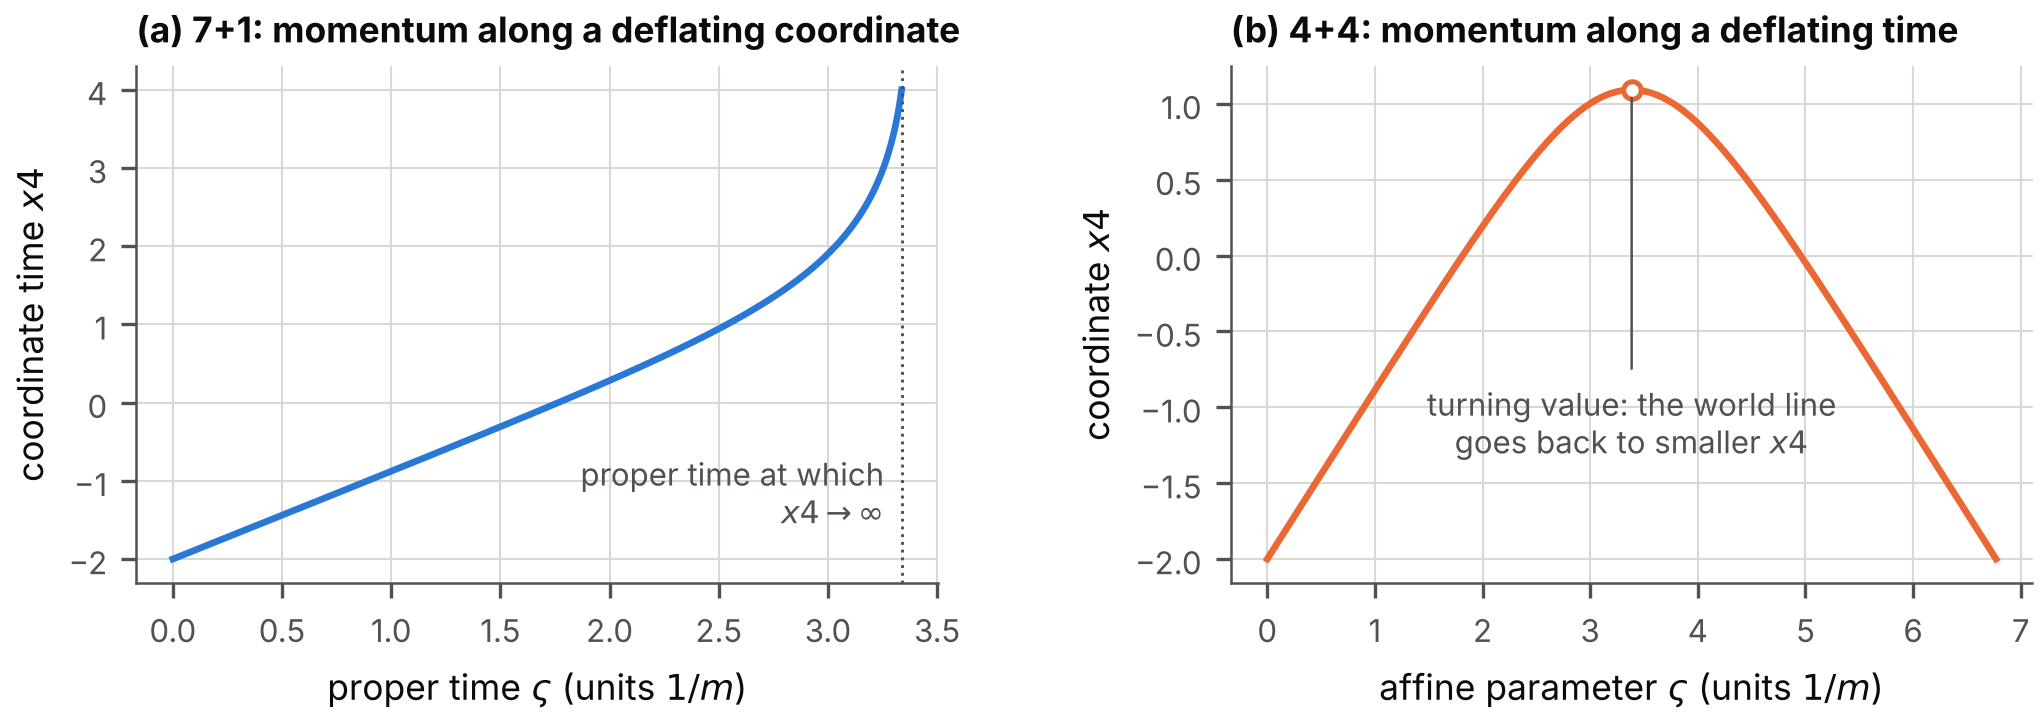
\includegraphics[width=0.85\textwidth,height=\textheight]{figures/fig_geodesics.png}
\caption{A classical particle of the mass \(m=1\) with the momenta
\(P_1=0.5\) along \(x1\) and \(P_5=0.3\) along the deflating coordinate
\(x5\), for \(\mathrm{g55}=1\) and \(\mathrm{const}_5=0.8\), started at
\(x4=-2\). (a) On the 7+1 spacetime the time \(x4\) grows without bound
within the finite proper time 3.386. (b) On the 4+4 spacetime the path
reaches the turning value \(x4=1.0924\) and returns to smaller \(x4\).}
\end{figure}

\begin{center}\rule{0.5\linewidth}{0.5pt}\end{center}

\hypertarget{part-2.-dirac-matrices-and-spin-connection}{%
\section{Part 2. Dirac matrices and spin
connection}\label{part-2.-dirac-matrices-and-spin-connection}}

\hypertarget{the-dirac-matrices-of-the-orthonormal-frame}{%
\subsection{2.1 The Dirac matrices of the orthonormal
frame}\label{the-dirac-matrices-of-the-orthonormal-frame}}

At each point of a curved spacetime the tangent space is flat. The Dirac
matrices of the orthonormal frame are therefore eight \emph{constant}
matrices \(\gamma^A\), \(A=0,\dots,7\), the same at every point. For
each of the two spacetimes they are real \(16\times16\) matrices with
entries \(0\) and \(\pm1\); each is a signed permutation matrix. They
are written \(\gamma_{1644}^A\) and \(\gamma_{1671}^A\) where the two
sets must be distinguished, and \(\gamma^A\) where a statement holds for
either set. They satisfy

\[\gamma^A\gamma^B+\gamma^B\gamma^A=2\,c_\gamma\,\eta^{AB}\,1,\qquad
c_\gamma=+1\ \text{(4+4)},\qquad c_\gamma=-1\ \text{(7+1)},\tag{2.1}\]

with the flat metric (1.1) of the spacetime concerned. Written out:
different matrices anticommute, and the squares are as follows
(\(j=0,1,2,3\) and \(t=5,6,7\)).

\begin{longtable}[]{@{}
  >{\raggedright\arraybackslash}p{(\columnwidth - 10\tabcolsep) * \real{0.1667}}
  >{\raggedright\arraybackslash}p{(\columnwidth - 10\tabcolsep) * \real{0.1667}}
  >{\raggedright\arraybackslash}p{(\columnwidth - 10\tabcolsep) * \real{0.1667}}
  >{\raggedright\arraybackslash}p{(\columnwidth - 10\tabcolsep) * \real{0.1667}}
  >{\raggedright\arraybackslash}p{(\columnwidth - 10\tabcolsep) * \real{0.1667}}
  >{\raggedright\arraybackslash}p{(\columnwidth - 10\tabcolsep) * \real{0.1667}}@{}}
\toprule\noalign{}
\begin{minipage}[b]{\linewidth}\raggedright
set
\end{minipage} & \begin{minipage}[b]{\linewidth}\raggedright
\((\gamma^j)^2\)
\end{minipage} & \begin{minipage}[b]{\linewidth}\raggedright
\((\gamma^4)^2\)
\end{minipage} & \begin{minipage}[b]{\linewidth}\raggedright
\((\gamma^t)^2\)
\end{minipage} & \begin{minipage}[b]{\linewidth}\raggedright
symmetric
\end{minipage} & \begin{minipage}[b]{\linewidth}\raggedright
antisymmetric
\end{minipage} \\
\midrule\noalign{}
\endhead
\bottomrule\noalign{}
\endlastfoot
\(\gamma_{1644}^A\) & \(+1\) & \(-1\) & \(-1\) &
\(\gamma^0,\dots,\gamma^3\) & \(\gamma^4,\dots,\gamma^7\) \\
\(\gamma_{1671}^A\) & \(-1\) & \(+1\) & \(-1\) & \(\gamma^4\) & the
seven others \\
\end{longtable}

The matrices of the 4+4 spacetime square to the sign of the metric.
Those of the 7+1 spacetime square to \emph{minus} the sign of the
metric: the matrix of the time squares to \(+1\), as in the familiar
Dirac theory with the metric \((+,-,-,-)\), while this document writes
the metric with space-like components positive. The constant
\(c_\gamma=-1\) records this, and it accompanies the 7+1 matrices
through all formulas (checks \texttt{44-R1}, \texttt{44-R2},
\texttt{44-C1}, \texttt{44-C2} and \texttt{71-R1}, \texttt{71-R2},
\texttt{71-C1}, \texttt{71-C2} of the report on the matrices of the
frame, Appendix A.2, and \texttt{44d-C1}, \texttt{71d-C1}). In the
reports of the programs the diagonal matrices of these squares are
called \texttt{eta1644} and \texttt{eta1671}, in formulas
\(\eta_{1644}\) and \(\eta_{1671}\); they are related to the flat
metrics (1.1) by \(\eta_{1644}=\eta^{(4+4)}\) and
\(\eta_{1671}=-\eta^{(7+1)}\).

\hypertarget{the-eight-matrices-of-the-44-spacetime}{%
\subsubsection{The eight matrices of the 4+4
spacetime}\label{the-eight-matrices-of-the-44-spacetime}}

In the following displays \(+\) stands for \(+1\), \(-\) for \(-1\) and
a dot for \(0\).

\[\gamma_{1644}^0=\left(\begin{smallmatrix} \cdot & \cdot & \cdot & \cdot & \cdot & \cdot & \cdot & \cdot & + & \cdot & \cdot & \cdot & \cdot & \cdot & \cdot & \cdot \\ \cdot & \cdot & \cdot & \cdot & \cdot & \cdot & \cdot & \cdot & \cdot & + & \cdot & \cdot & \cdot & \cdot & \cdot & \cdot \\ \cdot & \cdot & \cdot & \cdot & \cdot & \cdot & \cdot & \cdot & \cdot & \cdot & + & \cdot & \cdot & \cdot & \cdot & \cdot \\ \cdot & \cdot & \cdot & \cdot & \cdot & \cdot & \cdot & \cdot & \cdot & \cdot & \cdot & + & \cdot & \cdot & \cdot & \cdot \\ \cdot & \cdot & \cdot & \cdot & \cdot & \cdot & \cdot & \cdot & \cdot & \cdot & \cdot & \cdot & + & \cdot & \cdot & \cdot \\ \cdot & \cdot & \cdot & \cdot & \cdot & \cdot & \cdot & \cdot & \cdot & \cdot & \cdot & \cdot & \cdot & + & \cdot & \cdot \\ \cdot & \cdot & \cdot & \cdot & \cdot & \cdot & \cdot & \cdot & \cdot & \cdot & \cdot & \cdot & \cdot & \cdot & + & \cdot \\ \cdot & \cdot & \cdot & \cdot & \cdot & \cdot & \cdot & \cdot & \cdot & \cdot & \cdot & \cdot & \cdot & \cdot & \cdot & + \\ + & \cdot & \cdot & \cdot & \cdot & \cdot & \cdot & \cdot & \cdot & \cdot & \cdot & \cdot & \cdot & \cdot & \cdot & \cdot \\ \cdot & + & \cdot & \cdot & \cdot & \cdot & \cdot & \cdot & \cdot & \cdot & \cdot & \cdot & \cdot & \cdot & \cdot & \cdot \\ \cdot & \cdot & + & \cdot & \cdot & \cdot & \cdot & \cdot & \cdot & \cdot & \cdot & \cdot & \cdot & \cdot & \cdot & \cdot \\ \cdot & \cdot & \cdot & + & \cdot & \cdot & \cdot & \cdot & \cdot & \cdot & \cdot & \cdot & \cdot & \cdot & \cdot & \cdot \\ \cdot & \cdot & \cdot & \cdot & + & \cdot & \cdot & \cdot & \cdot & \cdot & \cdot & \cdot & \cdot & \cdot & \cdot & \cdot \\ \cdot & \cdot & \cdot & \cdot & \cdot & + & \cdot & \cdot & \cdot & \cdot & \cdot & \cdot & \cdot & \cdot & \cdot & \cdot \\ \cdot & \cdot & \cdot & \cdot & \cdot & \cdot & + & \cdot & \cdot & \cdot & \cdot & \cdot & \cdot & \cdot & \cdot & \cdot \\ \cdot & \cdot & \cdot & \cdot & \cdot & \cdot & \cdot & + & \cdot & \cdot & \cdot & \cdot & \cdot & \cdot & \cdot & \cdot \end{smallmatrix}\right)\qquad
\gamma_{1644}^1=\left(\begin{smallmatrix} \cdot & \cdot & \cdot & \cdot & \cdot & \cdot & \cdot & \cdot & \cdot & \cdot & \cdot & \cdot & \cdot & \cdot & \cdot & - \\ \cdot & \cdot & \cdot & \cdot & \cdot & \cdot & \cdot & \cdot & \cdot & \cdot & \cdot & \cdot & \cdot & \cdot & - & \cdot \\ \cdot & \cdot & \cdot & \cdot & \cdot & \cdot & \cdot & \cdot & \cdot & \cdot & \cdot & \cdot & \cdot & + & \cdot & \cdot \\ \cdot & \cdot & \cdot & \cdot & \cdot & \cdot & \cdot & \cdot & \cdot & \cdot & \cdot & \cdot & + & \cdot & \cdot & \cdot \\ \cdot & \cdot & \cdot & \cdot & \cdot & \cdot & \cdot & \cdot & \cdot & \cdot & \cdot & - & \cdot & \cdot & \cdot & \cdot \\ \cdot & \cdot & \cdot & \cdot & \cdot & \cdot & \cdot & \cdot & \cdot & \cdot & - & \cdot & \cdot & \cdot & \cdot & \cdot \\ \cdot & \cdot & \cdot & \cdot & \cdot & \cdot & \cdot & \cdot & \cdot & + & \cdot & \cdot & \cdot & \cdot & \cdot & \cdot \\ \cdot & \cdot & \cdot & \cdot & \cdot & \cdot & \cdot & \cdot & + & \cdot & \cdot & \cdot & \cdot & \cdot & \cdot & \cdot \\ \cdot & \cdot & \cdot & \cdot & \cdot & \cdot & \cdot & + & \cdot & \cdot & \cdot & \cdot & \cdot & \cdot & \cdot & \cdot \\ \cdot & \cdot & \cdot & \cdot & \cdot & \cdot & + & \cdot & \cdot & \cdot & \cdot & \cdot & \cdot & \cdot & \cdot & \cdot \\ \cdot & \cdot & \cdot & \cdot & \cdot & - & \cdot & \cdot & \cdot & \cdot & \cdot & \cdot & \cdot & \cdot & \cdot & \cdot \\ \cdot & \cdot & \cdot & \cdot & - & \cdot & \cdot & \cdot & \cdot & \cdot & \cdot & \cdot & \cdot & \cdot & \cdot & \cdot \\ \cdot & \cdot & \cdot & + & \cdot & \cdot & \cdot & \cdot & \cdot & \cdot & \cdot & \cdot & \cdot & \cdot & \cdot & \cdot \\ \cdot & \cdot & + & \cdot & \cdot & \cdot & \cdot & \cdot & \cdot & \cdot & \cdot & \cdot & \cdot & \cdot & \cdot & \cdot \\ \cdot & - & \cdot & \cdot & \cdot & \cdot & \cdot & \cdot & \cdot & \cdot & \cdot & \cdot & \cdot & \cdot & \cdot & \cdot \\ - & \cdot & \cdot & \cdot & \cdot & \cdot & \cdot & \cdot & \cdot & \cdot & \cdot & \cdot & \cdot & \cdot & \cdot & \cdot \end{smallmatrix}\right)\]

\[\gamma_{1644}^2=\left(\begin{smallmatrix} \cdot & \cdot & \cdot & \cdot & \cdot & \cdot & \cdot & \cdot & \cdot & \cdot & \cdot & \cdot & \cdot & \cdot & + & \cdot \\ \cdot & \cdot & \cdot & \cdot & \cdot & \cdot & \cdot & \cdot & \cdot & \cdot & \cdot & \cdot & \cdot & \cdot & \cdot & - \\ \cdot & \cdot & \cdot & \cdot & \cdot & \cdot & \cdot & \cdot & \cdot & \cdot & \cdot & \cdot & - & \cdot & \cdot & \cdot \\ \cdot & \cdot & \cdot & \cdot & \cdot & \cdot & \cdot & \cdot & \cdot & \cdot & \cdot & \cdot & \cdot & + & \cdot & \cdot \\ \cdot & \cdot & \cdot & \cdot & \cdot & \cdot & \cdot & \cdot & \cdot & \cdot & + & \cdot & \cdot & \cdot & \cdot & \cdot \\ \cdot & \cdot & \cdot & \cdot & \cdot & \cdot & \cdot & \cdot & \cdot & \cdot & \cdot & - & \cdot & \cdot & \cdot & \cdot \\ \cdot & \cdot & \cdot & \cdot & \cdot & \cdot & \cdot & \cdot & - & \cdot & \cdot & \cdot & \cdot & \cdot & \cdot & \cdot \\ \cdot & \cdot & \cdot & \cdot & \cdot & \cdot & \cdot & \cdot & \cdot & + & \cdot & \cdot & \cdot & \cdot & \cdot & \cdot \\ \cdot & \cdot & \cdot & \cdot & \cdot & \cdot & - & \cdot & \cdot & \cdot & \cdot & \cdot & \cdot & \cdot & \cdot & \cdot \\ \cdot & \cdot & \cdot & \cdot & \cdot & \cdot & \cdot & + & \cdot & \cdot & \cdot & \cdot & \cdot & \cdot & \cdot & \cdot \\ \cdot & \cdot & \cdot & \cdot & + & \cdot & \cdot & \cdot & \cdot & \cdot & \cdot & \cdot & \cdot & \cdot & \cdot & \cdot \\ \cdot & \cdot & \cdot & \cdot & \cdot & - & \cdot & \cdot & \cdot & \cdot & \cdot & \cdot & \cdot & \cdot & \cdot & \cdot \\ \cdot & \cdot & - & \cdot & \cdot & \cdot & \cdot & \cdot & \cdot & \cdot & \cdot & \cdot & \cdot & \cdot & \cdot & \cdot \\ \cdot & \cdot & \cdot & + & \cdot & \cdot & \cdot & \cdot & \cdot & \cdot & \cdot & \cdot & \cdot & \cdot & \cdot & \cdot \\ + & \cdot & \cdot & \cdot & \cdot & \cdot & \cdot & \cdot & \cdot & \cdot & \cdot & \cdot & \cdot & \cdot & \cdot & \cdot \\ \cdot & - & \cdot & \cdot & \cdot & \cdot & \cdot & \cdot & \cdot & \cdot & \cdot & \cdot & \cdot & \cdot & \cdot & \cdot \end{smallmatrix}\right)\qquad
\gamma_{1644}^3=\left(\begin{smallmatrix} \cdot & \cdot & \cdot & \cdot & \cdot & \cdot & \cdot & \cdot & \cdot & \cdot & \cdot & \cdot & \cdot & - & \cdot & \cdot \\ \cdot & \cdot & \cdot & \cdot & \cdot & \cdot & \cdot & \cdot & \cdot & \cdot & \cdot & \cdot & + & \cdot & \cdot & \cdot \\ \cdot & \cdot & \cdot & \cdot & \cdot & \cdot & \cdot & \cdot & \cdot & \cdot & \cdot & \cdot & \cdot & \cdot & \cdot & - \\ \cdot & \cdot & \cdot & \cdot & \cdot & \cdot & \cdot & \cdot & \cdot & \cdot & \cdot & \cdot & \cdot & \cdot & + & \cdot \\ \cdot & \cdot & \cdot & \cdot & \cdot & \cdot & \cdot & \cdot & \cdot & - & \cdot & \cdot & \cdot & \cdot & \cdot & \cdot \\ \cdot & \cdot & \cdot & \cdot & \cdot & \cdot & \cdot & \cdot & + & \cdot & \cdot & \cdot & \cdot & \cdot & \cdot & \cdot \\ \cdot & \cdot & \cdot & \cdot & \cdot & \cdot & \cdot & \cdot & \cdot & \cdot & \cdot & - & \cdot & \cdot & \cdot & \cdot \\ \cdot & \cdot & \cdot & \cdot & \cdot & \cdot & \cdot & \cdot & \cdot & \cdot & + & \cdot & \cdot & \cdot & \cdot & \cdot \\ \cdot & \cdot & \cdot & \cdot & \cdot & + & \cdot & \cdot & \cdot & \cdot & \cdot & \cdot & \cdot & \cdot & \cdot & \cdot \\ \cdot & \cdot & \cdot & \cdot & - & \cdot & \cdot & \cdot & \cdot & \cdot & \cdot & \cdot & \cdot & \cdot & \cdot & \cdot \\ \cdot & \cdot & \cdot & \cdot & \cdot & \cdot & \cdot & + & \cdot & \cdot & \cdot & \cdot & \cdot & \cdot & \cdot & \cdot \\ \cdot & \cdot & \cdot & \cdot & \cdot & \cdot & - & \cdot & \cdot & \cdot & \cdot & \cdot & \cdot & \cdot & \cdot & \cdot \\ \cdot & + & \cdot & \cdot & \cdot & \cdot & \cdot & \cdot & \cdot & \cdot & \cdot & \cdot & \cdot & \cdot & \cdot & \cdot \\ - & \cdot & \cdot & \cdot & \cdot & \cdot & \cdot & \cdot & \cdot & \cdot & \cdot & \cdot & \cdot & \cdot & \cdot & \cdot \\ \cdot & \cdot & \cdot & + & \cdot & \cdot & \cdot & \cdot & \cdot & \cdot & \cdot & \cdot & \cdot & \cdot & \cdot & \cdot \\ \cdot & \cdot & - & \cdot & \cdot & \cdot & \cdot & \cdot & \cdot & \cdot & \cdot & \cdot & \cdot & \cdot & \cdot & \cdot \end{smallmatrix}\right)\]

\[\gamma_{1644}^4=\left(\begin{smallmatrix} \cdot & \cdot & \cdot & \cdot & \cdot & \cdot & \cdot & \cdot & \cdot & \cdot & \cdot & \cdot & \cdot & - & \cdot & \cdot \\ \cdot & \cdot & \cdot & \cdot & \cdot & \cdot & \cdot & \cdot & \cdot & \cdot & \cdot & \cdot & + & \cdot & \cdot & \cdot \\ \cdot & \cdot & \cdot & \cdot & \cdot & \cdot & \cdot & \cdot & \cdot & \cdot & \cdot & \cdot & \cdot & \cdot & \cdot & + \\ \cdot & \cdot & \cdot & \cdot & \cdot & \cdot & \cdot & \cdot & \cdot & \cdot & \cdot & \cdot & \cdot & \cdot & - & \cdot \\ \cdot & \cdot & \cdot & \cdot & \cdot & \cdot & \cdot & \cdot & \cdot & + & \cdot & \cdot & \cdot & \cdot & \cdot & \cdot \\ \cdot & \cdot & \cdot & \cdot & \cdot & \cdot & \cdot & \cdot & - & \cdot & \cdot & \cdot & \cdot & \cdot & \cdot & \cdot \\ \cdot & \cdot & \cdot & \cdot & \cdot & \cdot & \cdot & \cdot & \cdot & \cdot & \cdot & - & \cdot & \cdot & \cdot & \cdot \\ \cdot & \cdot & \cdot & \cdot & \cdot & \cdot & \cdot & \cdot & \cdot & \cdot & + & \cdot & \cdot & \cdot & \cdot & \cdot \\ \cdot & \cdot & \cdot & \cdot & \cdot & + & \cdot & \cdot & \cdot & \cdot & \cdot & \cdot & \cdot & \cdot & \cdot & \cdot \\ \cdot & \cdot & \cdot & \cdot & - & \cdot & \cdot & \cdot & \cdot & \cdot & \cdot & \cdot & \cdot & \cdot & \cdot & \cdot \\ \cdot & \cdot & \cdot & \cdot & \cdot & \cdot & \cdot & - & \cdot & \cdot & \cdot & \cdot & \cdot & \cdot & \cdot & \cdot \\ \cdot & \cdot & \cdot & \cdot & \cdot & \cdot & + & \cdot & \cdot & \cdot & \cdot & \cdot & \cdot & \cdot & \cdot & \cdot \\ \cdot & - & \cdot & \cdot & \cdot & \cdot & \cdot & \cdot & \cdot & \cdot & \cdot & \cdot & \cdot & \cdot & \cdot & \cdot \\ + & \cdot & \cdot & \cdot & \cdot & \cdot & \cdot & \cdot & \cdot & \cdot & \cdot & \cdot & \cdot & \cdot & \cdot & \cdot \\ \cdot & \cdot & \cdot & + & \cdot & \cdot & \cdot & \cdot & \cdot & \cdot & \cdot & \cdot & \cdot & \cdot & \cdot & \cdot \\ \cdot & \cdot & - & \cdot & \cdot & \cdot & \cdot & \cdot & \cdot & \cdot & \cdot & \cdot & \cdot & \cdot & \cdot & \cdot \end{smallmatrix}\right)\qquad
\gamma_{1644}^5=\left(\begin{smallmatrix} \cdot & \cdot & \cdot & \cdot & \cdot & \cdot & \cdot & \cdot & \cdot & \cdot & \cdot & \cdot & \cdot & \cdot & + & \cdot \\ \cdot & \cdot & \cdot & \cdot & \cdot & \cdot & \cdot & \cdot & \cdot & \cdot & \cdot & \cdot & \cdot & \cdot & \cdot & + \\ \cdot & \cdot & \cdot & \cdot & \cdot & \cdot & \cdot & \cdot & \cdot & \cdot & \cdot & \cdot & - & \cdot & \cdot & \cdot \\ \cdot & \cdot & \cdot & \cdot & \cdot & \cdot & \cdot & \cdot & \cdot & \cdot & \cdot & \cdot & \cdot & - & \cdot & \cdot \\ \cdot & \cdot & \cdot & \cdot & \cdot & \cdot & \cdot & \cdot & \cdot & \cdot & - & \cdot & \cdot & \cdot & \cdot & \cdot \\ \cdot & \cdot & \cdot & \cdot & \cdot & \cdot & \cdot & \cdot & \cdot & \cdot & \cdot & - & \cdot & \cdot & \cdot & \cdot \\ \cdot & \cdot & \cdot & \cdot & \cdot & \cdot & \cdot & \cdot & + & \cdot & \cdot & \cdot & \cdot & \cdot & \cdot & \cdot \\ \cdot & \cdot & \cdot & \cdot & \cdot & \cdot & \cdot & \cdot & \cdot & + & \cdot & \cdot & \cdot & \cdot & \cdot & \cdot \\ \cdot & \cdot & \cdot & \cdot & \cdot & \cdot & - & \cdot & \cdot & \cdot & \cdot & \cdot & \cdot & \cdot & \cdot & \cdot \\ \cdot & \cdot & \cdot & \cdot & \cdot & \cdot & \cdot & - & \cdot & \cdot & \cdot & \cdot & \cdot & \cdot & \cdot & \cdot \\ \cdot & \cdot & \cdot & \cdot & + & \cdot & \cdot & \cdot & \cdot & \cdot & \cdot & \cdot & \cdot & \cdot & \cdot & \cdot \\ \cdot & \cdot & \cdot & \cdot & \cdot & + & \cdot & \cdot & \cdot & \cdot & \cdot & \cdot & \cdot & \cdot & \cdot & \cdot \\ \cdot & \cdot & + & \cdot & \cdot & \cdot & \cdot & \cdot & \cdot & \cdot & \cdot & \cdot & \cdot & \cdot & \cdot & \cdot \\ \cdot & \cdot & \cdot & + & \cdot & \cdot & \cdot & \cdot & \cdot & \cdot & \cdot & \cdot & \cdot & \cdot & \cdot & \cdot \\ - & \cdot & \cdot & \cdot & \cdot & \cdot & \cdot & \cdot & \cdot & \cdot & \cdot & \cdot & \cdot & \cdot & \cdot & \cdot \\ \cdot & - & \cdot & \cdot & \cdot & \cdot & \cdot & \cdot & \cdot & \cdot & \cdot & \cdot & \cdot & \cdot & \cdot & \cdot \end{smallmatrix}\right)\]

\[\gamma_{1644}^6=\left(\begin{smallmatrix} \cdot & \cdot & \cdot & \cdot & \cdot & \cdot & \cdot & \cdot & \cdot & \cdot & \cdot & \cdot & \cdot & \cdot & \cdot & + \\ \cdot & \cdot & \cdot & \cdot & \cdot & \cdot & \cdot & \cdot & \cdot & \cdot & \cdot & \cdot & \cdot & \cdot & - & \cdot \\ \cdot & \cdot & \cdot & \cdot & \cdot & \cdot & \cdot & \cdot & \cdot & \cdot & \cdot & \cdot & \cdot & + & \cdot & \cdot \\ \cdot & \cdot & \cdot & \cdot & \cdot & \cdot & \cdot & \cdot & \cdot & \cdot & \cdot & \cdot & - & \cdot & \cdot & \cdot \\ \cdot & \cdot & \cdot & \cdot & \cdot & \cdot & \cdot & \cdot & \cdot & \cdot & \cdot & - & \cdot & \cdot & \cdot & \cdot \\ \cdot & \cdot & \cdot & \cdot & \cdot & \cdot & \cdot & \cdot & \cdot & \cdot & + & \cdot & \cdot & \cdot & \cdot & \cdot \\ \cdot & \cdot & \cdot & \cdot & \cdot & \cdot & \cdot & \cdot & \cdot & - & \cdot & \cdot & \cdot & \cdot & \cdot & \cdot \\ \cdot & \cdot & \cdot & \cdot & \cdot & \cdot & \cdot & \cdot & + & \cdot & \cdot & \cdot & \cdot & \cdot & \cdot & \cdot \\ \cdot & \cdot & \cdot & \cdot & \cdot & \cdot & \cdot & - & \cdot & \cdot & \cdot & \cdot & \cdot & \cdot & \cdot & \cdot \\ \cdot & \cdot & \cdot & \cdot & \cdot & \cdot & + & \cdot & \cdot & \cdot & \cdot & \cdot & \cdot & \cdot & \cdot & \cdot \\ \cdot & \cdot & \cdot & \cdot & \cdot & - & \cdot & \cdot & \cdot & \cdot & \cdot & \cdot & \cdot & \cdot & \cdot & \cdot \\ \cdot & \cdot & \cdot & \cdot & + & \cdot & \cdot & \cdot & \cdot & \cdot & \cdot & \cdot & \cdot & \cdot & \cdot & \cdot \\ \cdot & \cdot & \cdot & + & \cdot & \cdot & \cdot & \cdot & \cdot & \cdot & \cdot & \cdot & \cdot & \cdot & \cdot & \cdot \\ \cdot & \cdot & - & \cdot & \cdot & \cdot & \cdot & \cdot & \cdot & \cdot & \cdot & \cdot & \cdot & \cdot & \cdot & \cdot \\ \cdot & + & \cdot & \cdot & \cdot & \cdot & \cdot & \cdot & \cdot & \cdot & \cdot & \cdot & \cdot & \cdot & \cdot & \cdot \\ - & \cdot & \cdot & \cdot & \cdot & \cdot & \cdot & \cdot & \cdot & \cdot & \cdot & \cdot & \cdot & \cdot & \cdot & \cdot \end{smallmatrix}\right)\qquad
\gamma_{1644}^7=\left(\begin{smallmatrix} \cdot & \cdot & \cdot & \cdot & \cdot & \cdot & \cdot & \cdot & + & \cdot & \cdot & \cdot & \cdot & \cdot & \cdot & \cdot \\ \cdot & \cdot & \cdot & \cdot & \cdot & \cdot & \cdot & \cdot & \cdot & + & \cdot & \cdot & \cdot & \cdot & \cdot & \cdot \\ \cdot & \cdot & \cdot & \cdot & \cdot & \cdot & \cdot & \cdot & \cdot & \cdot & + & \cdot & \cdot & \cdot & \cdot & \cdot \\ \cdot & \cdot & \cdot & \cdot & \cdot & \cdot & \cdot & \cdot & \cdot & \cdot & \cdot & + & \cdot & \cdot & \cdot & \cdot \\ \cdot & \cdot & \cdot & \cdot & \cdot & \cdot & \cdot & \cdot & \cdot & \cdot & \cdot & \cdot & - & \cdot & \cdot & \cdot \\ \cdot & \cdot & \cdot & \cdot & \cdot & \cdot & \cdot & \cdot & \cdot & \cdot & \cdot & \cdot & \cdot & - & \cdot & \cdot \\ \cdot & \cdot & \cdot & \cdot & \cdot & \cdot & \cdot & \cdot & \cdot & \cdot & \cdot & \cdot & \cdot & \cdot & - & \cdot \\ \cdot & \cdot & \cdot & \cdot & \cdot & \cdot & \cdot & \cdot & \cdot & \cdot & \cdot & \cdot & \cdot & \cdot & \cdot & - \\ - & \cdot & \cdot & \cdot & \cdot & \cdot & \cdot & \cdot & \cdot & \cdot & \cdot & \cdot & \cdot & \cdot & \cdot & \cdot \\ \cdot & - & \cdot & \cdot & \cdot & \cdot & \cdot & \cdot & \cdot & \cdot & \cdot & \cdot & \cdot & \cdot & \cdot & \cdot \\ \cdot & \cdot & - & \cdot & \cdot & \cdot & \cdot & \cdot & \cdot & \cdot & \cdot & \cdot & \cdot & \cdot & \cdot & \cdot \\ \cdot & \cdot & \cdot & - & \cdot & \cdot & \cdot & \cdot & \cdot & \cdot & \cdot & \cdot & \cdot & \cdot & \cdot & \cdot \\ \cdot & \cdot & \cdot & \cdot & + & \cdot & \cdot & \cdot & \cdot & \cdot & \cdot & \cdot & \cdot & \cdot & \cdot & \cdot \\ \cdot & \cdot & \cdot & \cdot & \cdot & + & \cdot & \cdot & \cdot & \cdot & \cdot & \cdot & \cdot & \cdot & \cdot & \cdot \\ \cdot & \cdot & \cdot & \cdot & \cdot & \cdot & + & \cdot & \cdot & \cdot & \cdot & \cdot & \cdot & \cdot & \cdot & \cdot \\ \cdot & \cdot & \cdot & \cdot & \cdot & \cdot & \cdot & + & \cdot & \cdot & \cdot & \cdot & \cdot & \cdot & \cdot & \cdot \end{smallmatrix}\right)\]

\[\omega_{1644}=\left(\begin{smallmatrix} - & \cdot & \cdot & \cdot & \cdot & \cdot & \cdot & \cdot & \cdot & \cdot & \cdot & \cdot & \cdot & \cdot & \cdot & \cdot \\ \cdot & - & \cdot & \cdot & \cdot & \cdot & \cdot & \cdot & \cdot & \cdot & \cdot & \cdot & \cdot & \cdot & \cdot & \cdot \\ \cdot & \cdot & - & \cdot & \cdot & \cdot & \cdot & \cdot & \cdot & \cdot & \cdot & \cdot & \cdot & \cdot & \cdot & \cdot \\ \cdot & \cdot & \cdot & - & \cdot & \cdot & \cdot & \cdot & \cdot & \cdot & \cdot & \cdot & \cdot & \cdot & \cdot & \cdot \\ \cdot & \cdot & \cdot & \cdot & - & \cdot & \cdot & \cdot & \cdot & \cdot & \cdot & \cdot & \cdot & \cdot & \cdot & \cdot \\ \cdot & \cdot & \cdot & \cdot & \cdot & - & \cdot & \cdot & \cdot & \cdot & \cdot & \cdot & \cdot & \cdot & \cdot & \cdot \\ \cdot & \cdot & \cdot & \cdot & \cdot & \cdot & - & \cdot & \cdot & \cdot & \cdot & \cdot & \cdot & \cdot & \cdot & \cdot \\ \cdot & \cdot & \cdot & \cdot & \cdot & \cdot & \cdot & - & \cdot & \cdot & \cdot & \cdot & \cdot & \cdot & \cdot & \cdot \\ \cdot & \cdot & \cdot & \cdot & \cdot & \cdot & \cdot & \cdot & + & \cdot & \cdot & \cdot & \cdot & \cdot & \cdot & \cdot \\ \cdot & \cdot & \cdot & \cdot & \cdot & \cdot & \cdot & \cdot & \cdot & + & \cdot & \cdot & \cdot & \cdot & \cdot & \cdot \\ \cdot & \cdot & \cdot & \cdot & \cdot & \cdot & \cdot & \cdot & \cdot & \cdot & + & \cdot & \cdot & \cdot & \cdot & \cdot \\ \cdot & \cdot & \cdot & \cdot & \cdot & \cdot & \cdot & \cdot & \cdot & \cdot & \cdot & + & \cdot & \cdot & \cdot & \cdot \\ \cdot & \cdot & \cdot & \cdot & \cdot & \cdot & \cdot & \cdot & \cdot & \cdot & \cdot & \cdot & + & \cdot & \cdot & \cdot \\ \cdot & \cdot & \cdot & \cdot & \cdot & \cdot & \cdot & \cdot & \cdot & \cdot & \cdot & \cdot & \cdot & + & \cdot & \cdot \\ \cdot & \cdot & \cdot & \cdot & \cdot & \cdot & \cdot & \cdot & \cdot & \cdot & \cdot & \cdot & \cdot & \cdot & + & \cdot \\ \cdot & \cdot & \cdot & \cdot & \cdot & \cdot & \cdot & \cdot & \cdot & \cdot & \cdot & \cdot & \cdot & \cdot & \cdot & + \end{smallmatrix}\right)\qquad
C^-_{1644}=\left(\begin{smallmatrix} \cdot & \cdot & \cdot & \cdot & - & \cdot & \cdot & \cdot & \cdot & \cdot & \cdot & \cdot & \cdot & \cdot & \cdot & \cdot \\ \cdot & \cdot & \cdot & \cdot & \cdot & - & \cdot & \cdot & \cdot & \cdot & \cdot & \cdot & \cdot & \cdot & \cdot & \cdot \\ \cdot & \cdot & \cdot & \cdot & \cdot & \cdot & - & \cdot & \cdot & \cdot & \cdot & \cdot & \cdot & \cdot & \cdot & \cdot \\ \cdot & \cdot & \cdot & \cdot & \cdot & \cdot & \cdot & - & \cdot & \cdot & \cdot & \cdot & \cdot & \cdot & \cdot & \cdot \\ - & \cdot & \cdot & \cdot & \cdot & \cdot & \cdot & \cdot & \cdot & \cdot & \cdot & \cdot & \cdot & \cdot & \cdot & \cdot \\ \cdot & - & \cdot & \cdot & \cdot & \cdot & \cdot & \cdot & \cdot & \cdot & \cdot & \cdot & \cdot & \cdot & \cdot & \cdot \\ \cdot & \cdot & - & \cdot & \cdot & \cdot & \cdot & \cdot & \cdot & \cdot & \cdot & \cdot & \cdot & \cdot & \cdot & \cdot \\ \cdot & \cdot & \cdot & - & \cdot & \cdot & \cdot & \cdot & \cdot & \cdot & \cdot & \cdot & \cdot & \cdot & \cdot & \cdot \\ \cdot & \cdot & \cdot & \cdot & \cdot & \cdot & \cdot & \cdot & \cdot & \cdot & \cdot & \cdot & + & \cdot & \cdot & \cdot \\ \cdot & \cdot & \cdot & \cdot & \cdot & \cdot & \cdot & \cdot & \cdot & \cdot & \cdot & \cdot & \cdot & + & \cdot & \cdot \\ \cdot & \cdot & \cdot & \cdot & \cdot & \cdot & \cdot & \cdot & \cdot & \cdot & \cdot & \cdot & \cdot & \cdot & + & \cdot \\ \cdot & \cdot & \cdot & \cdot & \cdot & \cdot & \cdot & \cdot & \cdot & \cdot & \cdot & \cdot & \cdot & \cdot & \cdot & + \\ \cdot & \cdot & \cdot & \cdot & \cdot & \cdot & \cdot & \cdot & + & \cdot & \cdot & \cdot & \cdot & \cdot & \cdot & \cdot \\ \cdot & \cdot & \cdot & \cdot & \cdot & \cdot & \cdot & \cdot & \cdot & + & \cdot & \cdot & \cdot & \cdot & \cdot & \cdot \\ \cdot & \cdot & \cdot & \cdot & \cdot & \cdot & \cdot & \cdot & \cdot & \cdot & + & \cdot & \cdot & \cdot & \cdot & \cdot \\ \cdot & \cdot & \cdot & \cdot & \cdot & \cdot & \cdot & \cdot & \cdot & \cdot & \cdot & + & \cdot & \cdot & \cdot & \cdot \end{smallmatrix}\right)\]

\[C^+_{1644}=\left(\begin{smallmatrix} \cdot & \cdot & \cdot & \cdot & + & \cdot & \cdot & \cdot & \cdot & \cdot & \cdot & \cdot & \cdot & \cdot & \cdot & \cdot \\ \cdot & \cdot & \cdot & \cdot & \cdot & + & \cdot & \cdot & \cdot & \cdot & \cdot & \cdot & \cdot & \cdot & \cdot & \cdot \\ \cdot & \cdot & \cdot & \cdot & \cdot & \cdot & + & \cdot & \cdot & \cdot & \cdot & \cdot & \cdot & \cdot & \cdot & \cdot \\ \cdot & \cdot & \cdot & \cdot & \cdot & \cdot & \cdot & + & \cdot & \cdot & \cdot & \cdot & \cdot & \cdot & \cdot & \cdot \\ + & \cdot & \cdot & \cdot & \cdot & \cdot & \cdot & \cdot & \cdot & \cdot & \cdot & \cdot & \cdot & \cdot & \cdot & \cdot \\ \cdot & + & \cdot & \cdot & \cdot & \cdot & \cdot & \cdot & \cdot & \cdot & \cdot & \cdot & \cdot & \cdot & \cdot & \cdot \\ \cdot & \cdot & + & \cdot & \cdot & \cdot & \cdot & \cdot & \cdot & \cdot & \cdot & \cdot & \cdot & \cdot & \cdot & \cdot \\ \cdot & \cdot & \cdot & + & \cdot & \cdot & \cdot & \cdot & \cdot & \cdot & \cdot & \cdot & \cdot & \cdot & \cdot & \cdot \\ \cdot & \cdot & \cdot & \cdot & \cdot & \cdot & \cdot & \cdot & \cdot & \cdot & \cdot & \cdot & + & \cdot & \cdot & \cdot \\ \cdot & \cdot & \cdot & \cdot & \cdot & \cdot & \cdot & \cdot & \cdot & \cdot & \cdot & \cdot & \cdot & + & \cdot & \cdot \\ \cdot & \cdot & \cdot & \cdot & \cdot & \cdot & \cdot & \cdot & \cdot & \cdot & \cdot & \cdot & \cdot & \cdot & + & \cdot \\ \cdot & \cdot & \cdot & \cdot & \cdot & \cdot & \cdot & \cdot & \cdot & \cdot & \cdot & \cdot & \cdot & \cdot & \cdot & + \\ \cdot & \cdot & \cdot & \cdot & \cdot & \cdot & \cdot & \cdot & + & \cdot & \cdot & \cdot & \cdot & \cdot & \cdot & \cdot \\ \cdot & \cdot & \cdot & \cdot & \cdot & \cdot & \cdot & \cdot & \cdot & + & \cdot & \cdot & \cdot & \cdot & \cdot & \cdot \\ \cdot & \cdot & \cdot & \cdot & \cdot & \cdot & \cdot & \cdot & \cdot & \cdot & + & \cdot & \cdot & \cdot & \cdot & \cdot \\ \cdot & \cdot & \cdot & \cdot & \cdot & \cdot & \cdot & \cdot & \cdot & \cdot & \cdot & + & \cdot & \cdot & \cdot & \cdot \end{smallmatrix}\right)\]

Matrices built from them (all verified in exact integer arithmetic):

\begin{longtable}[]{@{}
  >{\raggedright\arraybackslash}p{(\columnwidth - 4\tabcolsep) * \real{0.3333}}
  >{\raggedright\arraybackslash}p{(\columnwidth - 4\tabcolsep) * \real{0.3333}}
  >{\raggedright\arraybackslash}p{(\columnwidth - 4\tabcolsep) * \real{0.3333}}@{}}
\toprule\noalign{}
\begin{minipage}[b]{\linewidth}\raggedright
matrix
\end{minipage} & \begin{minipage}[b]{\linewidth}\raggedright
definition
\end{minipage} & \begin{minipage}[b]{\linewidth}\raggedright
properties
\end{minipage} \\
\midrule\noalign{}
\endhead
\bottomrule\noalign{}
\endlastfoot
\(\omega_{1644}\) & \(\gamma^0\gamma^1\cdots\gamma^7\) & real, diagonal,
\(\mathrm{diag}(-1_8,+1_8)\); anticommutes with every \(\gamma^A\); it
is the chirality matrix \(\chi\) of this spacetime \\
\(P^L\), \(P^R\) & \(\tfrac12(1-\chi)\), \(\tfrac12(1+\chi)\) & chiral
projectors; they select the upper and the lower eight components \\
\(C^-_{1644}\) & \(\gamma^0\gamma^1\gamma^2\gamma^3\) & real, symmetric,
square \(1\); \(C^-\gamma^A(C^-)^{-1}=-(\gamma^A)^T\); defines the
covariant adjoint \(\tilde\psi=\psi^\dagger C^-\) \\
\(C^+_{1644}\) & \(C^-\omega_{1644}\) &
\(C^+\gamma^A(C^+)^{-1}=+(\gamma^A)^T\) \\
\(\beta\) & \(-i\gamma^4\) & Hermitian, square \(1\) \\
\(\alpha^j\) & \(-\gamma^4\gamma^j\) (\(j=0,1,2,3\)) & Hermitian, square
\(1\); anticommute with one another and with \(\beta\) \\
\(W_{1644}\) & \(i\,C^-\gamma^4\) & Hermitian, square \(1\), trace
\(0\); commutes with \(\beta\) and with every \(\alpha^j\);
\(C^-=-W_{1644}\,\beta\) \\
\(\tau^A\), \(\bar\tau^A\) & the lower left and the upper right
\(8\times8\) block of \(\gamma^A\) & real;
\(\gamma^A=\begin{pmatrix}0&\bar\tau^A\\ \tau^A&0\end{pmatrix}\): every
\(\gamma^A\) exchanges the upper and the lower eight components \\
\end{longtable}

\hypertarget{the-eight-matrices-of-the-71-spacetime}{%
\subsubsection{The eight matrices of the 7+1
spacetime}\label{the-eight-matrices-of-the-71-spacetime}}

\[\gamma_{1671}^0=\left(\begin{smallmatrix} \cdot & - & \cdot & \cdot & \cdot & \cdot & \cdot & \cdot & \cdot & \cdot & \cdot & \cdot & \cdot & \cdot & \cdot & \cdot \\ + & \cdot & \cdot & \cdot & \cdot & \cdot & \cdot & \cdot & \cdot & \cdot & \cdot & \cdot & \cdot & \cdot & \cdot & \cdot \\ \cdot & \cdot & \cdot & + & \cdot & \cdot & \cdot & \cdot & \cdot & \cdot & \cdot & \cdot & \cdot & \cdot & \cdot & \cdot \\ \cdot & \cdot & - & \cdot & \cdot & \cdot & \cdot & \cdot & \cdot & \cdot & \cdot & \cdot & \cdot & \cdot & \cdot & \cdot \\ \cdot & \cdot & \cdot & \cdot & \cdot & + & \cdot & \cdot & \cdot & \cdot & \cdot & \cdot & \cdot & \cdot & \cdot & \cdot \\ \cdot & \cdot & \cdot & \cdot & - & \cdot & \cdot & \cdot & \cdot & \cdot & \cdot & \cdot & \cdot & \cdot & \cdot & \cdot \\ \cdot & \cdot & \cdot & \cdot & \cdot & \cdot & \cdot & - & \cdot & \cdot & \cdot & \cdot & \cdot & \cdot & \cdot & \cdot \\ \cdot & \cdot & \cdot & \cdot & \cdot & \cdot & + & \cdot & \cdot & \cdot & \cdot & \cdot & \cdot & \cdot & \cdot & \cdot \\ \cdot & \cdot & \cdot & \cdot & \cdot & \cdot & \cdot & \cdot & \cdot & + & \cdot & \cdot & \cdot & \cdot & \cdot & \cdot \\ \cdot & \cdot & \cdot & \cdot & \cdot & \cdot & \cdot & \cdot & - & \cdot & \cdot & \cdot & \cdot & \cdot & \cdot & \cdot \\ \cdot & \cdot & \cdot & \cdot & \cdot & \cdot & \cdot & \cdot & \cdot & \cdot & \cdot & - & \cdot & \cdot & \cdot & \cdot \\ \cdot & \cdot & \cdot & \cdot & \cdot & \cdot & \cdot & \cdot & \cdot & \cdot & + & \cdot & \cdot & \cdot & \cdot & \cdot \\ \cdot & \cdot & \cdot & \cdot & \cdot & \cdot & \cdot & \cdot & \cdot & \cdot & \cdot & \cdot & \cdot & - & \cdot & \cdot \\ \cdot & \cdot & \cdot & \cdot & \cdot & \cdot & \cdot & \cdot & \cdot & \cdot & \cdot & \cdot & + & \cdot & \cdot & \cdot \\ \cdot & \cdot & \cdot & \cdot & \cdot & \cdot & \cdot & \cdot & \cdot & \cdot & \cdot & \cdot & \cdot & \cdot & \cdot & + \\ \cdot & \cdot & \cdot & \cdot & \cdot & \cdot & \cdot & \cdot & \cdot & \cdot & \cdot & \cdot & \cdot & \cdot & - & \cdot \end{smallmatrix}\right)\qquad
\gamma_{1671}^1=\left(\begin{smallmatrix} \cdot & \cdot & \cdot & \cdot & \cdot & \cdot & \cdot & - & \cdot & \cdot & \cdot & \cdot & \cdot & \cdot & \cdot & \cdot \\ \cdot & \cdot & \cdot & \cdot & \cdot & \cdot & - & \cdot & \cdot & \cdot & \cdot & \cdot & \cdot & \cdot & \cdot & \cdot \\ \cdot & \cdot & \cdot & \cdot & \cdot & + & \cdot & \cdot & \cdot & \cdot & \cdot & \cdot & \cdot & \cdot & \cdot & \cdot \\ \cdot & \cdot & \cdot & \cdot & + & \cdot & \cdot & \cdot & \cdot & \cdot & \cdot & \cdot & \cdot & \cdot & \cdot & \cdot \\ \cdot & \cdot & \cdot & - & \cdot & \cdot & \cdot & \cdot & \cdot & \cdot & \cdot & \cdot & \cdot & \cdot & \cdot & \cdot \\ \cdot & \cdot & - & \cdot & \cdot & \cdot & \cdot & \cdot & \cdot & \cdot & \cdot & \cdot & \cdot & \cdot & \cdot & \cdot \\ \cdot & + & \cdot & \cdot & \cdot & \cdot & \cdot & \cdot & \cdot & \cdot & \cdot & \cdot & \cdot & \cdot & \cdot & \cdot \\ + & \cdot & \cdot & \cdot & \cdot & \cdot & \cdot & \cdot & \cdot & \cdot & \cdot & \cdot & \cdot & \cdot & \cdot & \cdot \\ \cdot & \cdot & \cdot & \cdot & \cdot & \cdot & \cdot & \cdot & \cdot & \cdot & \cdot & \cdot & \cdot & \cdot & \cdot & + \\ \cdot & \cdot & \cdot & \cdot & \cdot & \cdot & \cdot & \cdot & \cdot & \cdot & \cdot & \cdot & \cdot & \cdot & + & \cdot \\ \cdot & \cdot & \cdot & \cdot & \cdot & \cdot & \cdot & \cdot & \cdot & \cdot & \cdot & \cdot & \cdot & - & \cdot & \cdot \\ \cdot & \cdot & \cdot & \cdot & \cdot & \cdot & \cdot & \cdot & \cdot & \cdot & \cdot & \cdot & - & \cdot & \cdot & \cdot \\ \cdot & \cdot & \cdot & \cdot & \cdot & \cdot & \cdot & \cdot & \cdot & \cdot & \cdot & + & \cdot & \cdot & \cdot & \cdot \\ \cdot & \cdot & \cdot & \cdot & \cdot & \cdot & \cdot & \cdot & \cdot & \cdot & + & \cdot & \cdot & \cdot & \cdot & \cdot \\ \cdot & \cdot & \cdot & \cdot & \cdot & \cdot & \cdot & \cdot & \cdot & - & \cdot & \cdot & \cdot & \cdot & \cdot & \cdot \\ \cdot & \cdot & \cdot & \cdot & \cdot & \cdot & \cdot & \cdot & - & \cdot & \cdot & \cdot & \cdot & \cdot & \cdot & \cdot \end{smallmatrix}\right)\]

\[\gamma_{1671}^2=\left(\begin{smallmatrix} \cdot & \cdot & \cdot & \cdot & \cdot & \cdot & + & \cdot & \cdot & \cdot & \cdot & \cdot & \cdot & \cdot & \cdot & \cdot \\ \cdot & \cdot & \cdot & \cdot & \cdot & \cdot & \cdot & - & \cdot & \cdot & \cdot & \cdot & \cdot & \cdot & \cdot & \cdot \\ \cdot & \cdot & \cdot & \cdot & - & \cdot & \cdot & \cdot & \cdot & \cdot & \cdot & \cdot & \cdot & \cdot & \cdot & \cdot \\ \cdot & \cdot & \cdot & \cdot & \cdot & + & \cdot & \cdot & \cdot & \cdot & \cdot & \cdot & \cdot & \cdot & \cdot & \cdot \\ \cdot & \cdot & + & \cdot & \cdot & \cdot & \cdot & \cdot & \cdot & \cdot & \cdot & \cdot & \cdot & \cdot & \cdot & \cdot \\ \cdot & \cdot & \cdot & - & \cdot & \cdot & \cdot & \cdot & \cdot & \cdot & \cdot & \cdot & \cdot & \cdot & \cdot & \cdot \\ - & \cdot & \cdot & \cdot & \cdot & \cdot & \cdot & \cdot & \cdot & \cdot & \cdot & \cdot & \cdot & \cdot & \cdot & \cdot \\ \cdot & + & \cdot & \cdot & \cdot & \cdot & \cdot & \cdot & \cdot & \cdot & \cdot & \cdot & \cdot & \cdot & \cdot & \cdot \\ \cdot & \cdot & \cdot & \cdot & \cdot & \cdot & \cdot & \cdot & \cdot & \cdot & \cdot & \cdot & \cdot & \cdot & - & \cdot \\ \cdot & \cdot & \cdot & \cdot & \cdot & \cdot & \cdot & \cdot & \cdot & \cdot & \cdot & \cdot & \cdot & \cdot & \cdot & + \\ \cdot & \cdot & \cdot & \cdot & \cdot & \cdot & \cdot & \cdot & \cdot & \cdot & \cdot & \cdot & + & \cdot & \cdot & \cdot \\ \cdot & \cdot & \cdot & \cdot & \cdot & \cdot & \cdot & \cdot & \cdot & \cdot & \cdot & \cdot & \cdot & - & \cdot & \cdot \\ \cdot & \cdot & \cdot & \cdot & \cdot & \cdot & \cdot & \cdot & \cdot & \cdot & - & \cdot & \cdot & \cdot & \cdot & \cdot \\ \cdot & \cdot & \cdot & \cdot & \cdot & \cdot & \cdot & \cdot & \cdot & \cdot & \cdot & + & \cdot & \cdot & \cdot & \cdot \\ \cdot & \cdot & \cdot & \cdot & \cdot & \cdot & \cdot & \cdot & + & \cdot & \cdot & \cdot & \cdot & \cdot & \cdot & \cdot \\ \cdot & \cdot & \cdot & \cdot & \cdot & \cdot & \cdot & \cdot & \cdot & - & \cdot & \cdot & \cdot & \cdot & \cdot & \cdot \end{smallmatrix}\right)\qquad
\gamma_{1671}^3=\left(\begin{smallmatrix} \cdot & \cdot & \cdot & \cdot & \cdot & - & \cdot & \cdot & \cdot & \cdot & \cdot & \cdot & \cdot & \cdot & \cdot & \cdot \\ \cdot & \cdot & \cdot & \cdot & + & \cdot & \cdot & \cdot & \cdot & \cdot & \cdot & \cdot & \cdot & \cdot & \cdot & \cdot \\ \cdot & \cdot & \cdot & \cdot & \cdot & \cdot & \cdot & - & \cdot & \cdot & \cdot & \cdot & \cdot & \cdot & \cdot & \cdot \\ \cdot & \cdot & \cdot & \cdot & \cdot & \cdot & + & \cdot & \cdot & \cdot & \cdot & \cdot & \cdot & \cdot & \cdot & \cdot \\ \cdot & - & \cdot & \cdot & \cdot & \cdot & \cdot & \cdot & \cdot & \cdot & \cdot & \cdot & \cdot & \cdot & \cdot & \cdot \\ + & \cdot & \cdot & \cdot & \cdot & \cdot & \cdot & \cdot & \cdot & \cdot & \cdot & \cdot & \cdot & \cdot & \cdot & \cdot \\ \cdot & \cdot & \cdot & - & \cdot & \cdot & \cdot & \cdot & \cdot & \cdot & \cdot & \cdot & \cdot & \cdot & \cdot & \cdot \\ \cdot & \cdot & + & \cdot & \cdot & \cdot & \cdot & \cdot & \cdot & \cdot & \cdot & \cdot & \cdot & \cdot & \cdot & \cdot \\ \cdot & \cdot & \cdot & \cdot & \cdot & \cdot & \cdot & \cdot & \cdot & \cdot & \cdot & \cdot & \cdot & + & \cdot & \cdot \\ \cdot & \cdot & \cdot & \cdot & \cdot & \cdot & \cdot & \cdot & \cdot & \cdot & \cdot & \cdot & - & \cdot & \cdot & \cdot \\ \cdot & \cdot & \cdot & \cdot & \cdot & \cdot & \cdot & \cdot & \cdot & \cdot & \cdot & \cdot & \cdot & \cdot & \cdot & + \\ \cdot & \cdot & \cdot & \cdot & \cdot & \cdot & \cdot & \cdot & \cdot & \cdot & \cdot & \cdot & \cdot & \cdot & - & \cdot \\ \cdot & \cdot & \cdot & \cdot & \cdot & \cdot & \cdot & \cdot & \cdot & + & \cdot & \cdot & \cdot & \cdot & \cdot & \cdot \\ \cdot & \cdot & \cdot & \cdot & \cdot & \cdot & \cdot & \cdot & - & \cdot & \cdot & \cdot & \cdot & \cdot & \cdot & \cdot \\ \cdot & \cdot & \cdot & \cdot & \cdot & \cdot & \cdot & \cdot & \cdot & \cdot & \cdot & + & \cdot & \cdot & \cdot & \cdot \\ \cdot & \cdot & \cdot & \cdot & \cdot & \cdot & \cdot & \cdot & \cdot & \cdot & - & \cdot & \cdot & \cdot & \cdot & \cdot \end{smallmatrix}\right)\]

\[\gamma_{1671}^4=\left(\begin{smallmatrix} \cdot & \cdot & \cdot & \cdot & \cdot & \cdot & \cdot & \cdot & + & \cdot & \cdot & \cdot & \cdot & \cdot & \cdot & \cdot \\ \cdot & \cdot & \cdot & \cdot & \cdot & \cdot & \cdot & \cdot & \cdot & + & \cdot & \cdot & \cdot & \cdot & \cdot & \cdot \\ \cdot & \cdot & \cdot & \cdot & \cdot & \cdot & \cdot & \cdot & \cdot & \cdot & + & \cdot & \cdot & \cdot & \cdot & \cdot \\ \cdot & \cdot & \cdot & \cdot & \cdot & \cdot & \cdot & \cdot & \cdot & \cdot & \cdot & + & \cdot & \cdot & \cdot & \cdot \\ \cdot & \cdot & \cdot & \cdot & \cdot & \cdot & \cdot & \cdot & \cdot & \cdot & \cdot & \cdot & + & \cdot & \cdot & \cdot \\ \cdot & \cdot & \cdot & \cdot & \cdot & \cdot & \cdot & \cdot & \cdot & \cdot & \cdot & \cdot & \cdot & + & \cdot & \cdot \\ \cdot & \cdot & \cdot & \cdot & \cdot & \cdot & \cdot & \cdot & \cdot & \cdot & \cdot & \cdot & \cdot & \cdot & + & \cdot \\ \cdot & \cdot & \cdot & \cdot & \cdot & \cdot & \cdot & \cdot & \cdot & \cdot & \cdot & \cdot & \cdot & \cdot & \cdot & + \\ + & \cdot & \cdot & \cdot & \cdot & \cdot & \cdot & \cdot & \cdot & \cdot & \cdot & \cdot & \cdot & \cdot & \cdot & \cdot \\ \cdot & + & \cdot & \cdot & \cdot & \cdot & \cdot & \cdot & \cdot & \cdot & \cdot & \cdot & \cdot & \cdot & \cdot & \cdot \\ \cdot & \cdot & + & \cdot & \cdot & \cdot & \cdot & \cdot & \cdot & \cdot & \cdot & \cdot & \cdot & \cdot & \cdot & \cdot \\ \cdot & \cdot & \cdot & + & \cdot & \cdot & \cdot & \cdot & \cdot & \cdot & \cdot & \cdot & \cdot & \cdot & \cdot & \cdot \\ \cdot & \cdot & \cdot & \cdot & + & \cdot & \cdot & \cdot & \cdot & \cdot & \cdot & \cdot & \cdot & \cdot & \cdot & \cdot \\ \cdot & \cdot & \cdot & \cdot & \cdot & + & \cdot & \cdot & \cdot & \cdot & \cdot & \cdot & \cdot & \cdot & \cdot & \cdot \\ \cdot & \cdot & \cdot & \cdot & \cdot & \cdot & + & \cdot & \cdot & \cdot & \cdot & \cdot & \cdot & \cdot & \cdot & \cdot \\ \cdot & \cdot & \cdot & \cdot & \cdot & \cdot & \cdot & + & \cdot & \cdot & \cdot & \cdot & \cdot & \cdot & \cdot & \cdot \end{smallmatrix}\right)\qquad
\gamma_{1671}^5=\left(\begin{smallmatrix} \cdot & \cdot & + & \cdot & \cdot & \cdot & \cdot & \cdot & \cdot & \cdot & \cdot & \cdot & \cdot & \cdot & \cdot & \cdot \\ \cdot & \cdot & \cdot & + & \cdot & \cdot & \cdot & \cdot & \cdot & \cdot & \cdot & \cdot & \cdot & \cdot & \cdot & \cdot \\ - & \cdot & \cdot & \cdot & \cdot & \cdot & \cdot & \cdot & \cdot & \cdot & \cdot & \cdot & \cdot & \cdot & \cdot & \cdot \\ \cdot & - & \cdot & \cdot & \cdot & \cdot & \cdot & \cdot & \cdot & \cdot & \cdot & \cdot & \cdot & \cdot & \cdot & \cdot \\ \cdot & \cdot & \cdot & \cdot & \cdot & \cdot & - & \cdot & \cdot & \cdot & \cdot & \cdot & \cdot & \cdot & \cdot & \cdot \\ \cdot & \cdot & \cdot & \cdot & \cdot & \cdot & \cdot & - & \cdot & \cdot & \cdot & \cdot & \cdot & \cdot & \cdot & \cdot \\ \cdot & \cdot & \cdot & \cdot & + & \cdot & \cdot & \cdot & \cdot & \cdot & \cdot & \cdot & \cdot & \cdot & \cdot & \cdot \\ \cdot & \cdot & \cdot & \cdot & \cdot & + & \cdot & \cdot & \cdot & \cdot & \cdot & \cdot & \cdot & \cdot & \cdot & \cdot \\ \cdot & \cdot & \cdot & \cdot & \cdot & \cdot & \cdot & \cdot & \cdot & \cdot & - & \cdot & \cdot & \cdot & \cdot & \cdot \\ \cdot & \cdot & \cdot & \cdot & \cdot & \cdot & \cdot & \cdot & \cdot & \cdot & \cdot & - & \cdot & \cdot & \cdot & \cdot \\ \cdot & \cdot & \cdot & \cdot & \cdot & \cdot & \cdot & \cdot & + & \cdot & \cdot & \cdot & \cdot & \cdot & \cdot & \cdot \\ \cdot & \cdot & \cdot & \cdot & \cdot & \cdot & \cdot & \cdot & \cdot & + & \cdot & \cdot & \cdot & \cdot & \cdot & \cdot \\ \cdot & \cdot & \cdot & \cdot & \cdot & \cdot & \cdot & \cdot & \cdot & \cdot & \cdot & \cdot & \cdot & \cdot & + & \cdot \\ \cdot & \cdot & \cdot & \cdot & \cdot & \cdot & \cdot & \cdot & \cdot & \cdot & \cdot & \cdot & \cdot & \cdot & \cdot & + \\ \cdot & \cdot & \cdot & \cdot & \cdot & \cdot & \cdot & \cdot & \cdot & \cdot & \cdot & \cdot & - & \cdot & \cdot & \cdot \\ \cdot & \cdot & \cdot & \cdot & \cdot & \cdot & \cdot & \cdot & \cdot & \cdot & \cdot & \cdot & \cdot & - & \cdot & \cdot \end{smallmatrix}\right)\]

\[\gamma_{1671}^6=\left(\begin{smallmatrix} \cdot & \cdot & \cdot & + & \cdot & \cdot & \cdot & \cdot & \cdot & \cdot & \cdot & \cdot & \cdot & \cdot & \cdot & \cdot \\ \cdot & \cdot & - & \cdot & \cdot & \cdot & \cdot & \cdot & \cdot & \cdot & \cdot & \cdot & \cdot & \cdot & \cdot & \cdot \\ \cdot & + & \cdot & \cdot & \cdot & \cdot & \cdot & \cdot & \cdot & \cdot & \cdot & \cdot & \cdot & \cdot & \cdot & \cdot \\ - & \cdot & \cdot & \cdot & \cdot & \cdot & \cdot & \cdot & \cdot & \cdot & \cdot & \cdot & \cdot & \cdot & \cdot & \cdot \\ \cdot & \cdot & \cdot & \cdot & \cdot & \cdot & \cdot & - & \cdot & \cdot & \cdot & \cdot & \cdot & \cdot & \cdot & \cdot \\ \cdot & \cdot & \cdot & \cdot & \cdot & \cdot & + & \cdot & \cdot & \cdot & \cdot & \cdot & \cdot & \cdot & \cdot & \cdot \\ \cdot & \cdot & \cdot & \cdot & \cdot & - & \cdot & \cdot & \cdot & \cdot & \cdot & \cdot & \cdot & \cdot & \cdot & \cdot \\ \cdot & \cdot & \cdot & \cdot & + & \cdot & \cdot & \cdot & \cdot & \cdot & \cdot & \cdot & \cdot & \cdot & \cdot & \cdot \\ \cdot & \cdot & \cdot & \cdot & \cdot & \cdot & \cdot & \cdot & \cdot & \cdot & \cdot & - & \cdot & \cdot & \cdot & \cdot \\ \cdot & \cdot & \cdot & \cdot & \cdot & \cdot & \cdot & \cdot & \cdot & \cdot & + & \cdot & \cdot & \cdot & \cdot & \cdot \\ \cdot & \cdot & \cdot & \cdot & \cdot & \cdot & \cdot & \cdot & \cdot & - & \cdot & \cdot & \cdot & \cdot & \cdot & \cdot \\ \cdot & \cdot & \cdot & \cdot & \cdot & \cdot & \cdot & \cdot & + & \cdot & \cdot & \cdot & \cdot & \cdot & \cdot & \cdot \\ \cdot & \cdot & \cdot & \cdot & \cdot & \cdot & \cdot & \cdot & \cdot & \cdot & \cdot & \cdot & \cdot & \cdot & \cdot & + \\ \cdot & \cdot & \cdot & \cdot & \cdot & \cdot & \cdot & \cdot & \cdot & \cdot & \cdot & \cdot & \cdot & \cdot & - & \cdot \\ \cdot & \cdot & \cdot & \cdot & \cdot & \cdot & \cdot & \cdot & \cdot & \cdot & \cdot & \cdot & \cdot & + & \cdot & \cdot \\ \cdot & \cdot & \cdot & \cdot & \cdot & \cdot & \cdot & \cdot & \cdot & \cdot & \cdot & \cdot & - & \cdot & \cdot & \cdot \end{smallmatrix}\right)\qquad
\gamma_{1671}^7=\left(\begin{smallmatrix} \cdot & \cdot & \cdot & \cdot & + & \cdot & \cdot & \cdot & \cdot & \cdot & \cdot & \cdot & \cdot & \cdot & \cdot & \cdot \\ \cdot & \cdot & \cdot & \cdot & \cdot & + & \cdot & \cdot & \cdot & \cdot & \cdot & \cdot & \cdot & \cdot & \cdot & \cdot \\ \cdot & \cdot & \cdot & \cdot & \cdot & \cdot & + & \cdot & \cdot & \cdot & \cdot & \cdot & \cdot & \cdot & \cdot & \cdot \\ \cdot & \cdot & \cdot & \cdot & \cdot & \cdot & \cdot & + & \cdot & \cdot & \cdot & \cdot & \cdot & \cdot & \cdot & \cdot \\ - & \cdot & \cdot & \cdot & \cdot & \cdot & \cdot & \cdot & \cdot & \cdot & \cdot & \cdot & \cdot & \cdot & \cdot & \cdot \\ \cdot & - & \cdot & \cdot & \cdot & \cdot & \cdot & \cdot & \cdot & \cdot & \cdot & \cdot & \cdot & \cdot & \cdot & \cdot \\ \cdot & \cdot & - & \cdot & \cdot & \cdot & \cdot & \cdot & \cdot & \cdot & \cdot & \cdot & \cdot & \cdot & \cdot & \cdot \\ \cdot & \cdot & \cdot & - & \cdot & \cdot & \cdot & \cdot & \cdot & \cdot & \cdot & \cdot & \cdot & \cdot & \cdot & \cdot \\ \cdot & \cdot & \cdot & \cdot & \cdot & \cdot & \cdot & \cdot & \cdot & \cdot & \cdot & \cdot & - & \cdot & \cdot & \cdot \\ \cdot & \cdot & \cdot & \cdot & \cdot & \cdot & \cdot & \cdot & \cdot & \cdot & \cdot & \cdot & \cdot & - & \cdot & \cdot \\ \cdot & \cdot & \cdot & \cdot & \cdot & \cdot & \cdot & \cdot & \cdot & \cdot & \cdot & \cdot & \cdot & \cdot & - & \cdot \\ \cdot & \cdot & \cdot & \cdot & \cdot & \cdot & \cdot & \cdot & \cdot & \cdot & \cdot & \cdot & \cdot & \cdot & \cdot & - \\ \cdot & \cdot & \cdot & \cdot & \cdot & \cdot & \cdot & \cdot & + & \cdot & \cdot & \cdot & \cdot & \cdot & \cdot & \cdot \\ \cdot & \cdot & \cdot & \cdot & \cdot & \cdot & \cdot & \cdot & \cdot & + & \cdot & \cdot & \cdot & \cdot & \cdot & \cdot \\ \cdot & \cdot & \cdot & \cdot & \cdot & \cdot & \cdot & \cdot & \cdot & \cdot & + & \cdot & \cdot & \cdot & \cdot & \cdot \\ \cdot & \cdot & \cdot & \cdot & \cdot & \cdot & \cdot & \cdot & \cdot & \cdot & \cdot & + & \cdot & \cdot & \cdot & \cdot \end{smallmatrix}\right)\]

\[\omega_{1671}=\left(\begin{smallmatrix} \cdot & \cdot & \cdot & \cdot & \cdot & \cdot & \cdot & \cdot & - & \cdot & \cdot & \cdot & \cdot & \cdot & \cdot & \cdot \\ \cdot & \cdot & \cdot & \cdot & \cdot & \cdot & \cdot & \cdot & \cdot & - & \cdot & \cdot & \cdot & \cdot & \cdot & \cdot \\ \cdot & \cdot & \cdot & \cdot & \cdot & \cdot & \cdot & \cdot & \cdot & \cdot & - & \cdot & \cdot & \cdot & \cdot & \cdot \\ \cdot & \cdot & \cdot & \cdot & \cdot & \cdot & \cdot & \cdot & \cdot & \cdot & \cdot & - & \cdot & \cdot & \cdot & \cdot \\ \cdot & \cdot & \cdot & \cdot & \cdot & \cdot & \cdot & \cdot & \cdot & \cdot & \cdot & \cdot & - & \cdot & \cdot & \cdot \\ \cdot & \cdot & \cdot & \cdot & \cdot & \cdot & \cdot & \cdot & \cdot & \cdot & \cdot & \cdot & \cdot & - & \cdot & \cdot \\ \cdot & \cdot & \cdot & \cdot & \cdot & \cdot & \cdot & \cdot & \cdot & \cdot & \cdot & \cdot & \cdot & \cdot & - & \cdot \\ \cdot & \cdot & \cdot & \cdot & \cdot & \cdot & \cdot & \cdot & \cdot & \cdot & \cdot & \cdot & \cdot & \cdot & \cdot & - \\ + & \cdot & \cdot & \cdot & \cdot & \cdot & \cdot & \cdot & \cdot & \cdot & \cdot & \cdot & \cdot & \cdot & \cdot & \cdot \\ \cdot & + & \cdot & \cdot & \cdot & \cdot & \cdot & \cdot & \cdot & \cdot & \cdot & \cdot & \cdot & \cdot & \cdot & \cdot \\ \cdot & \cdot & + & \cdot & \cdot & \cdot & \cdot & \cdot & \cdot & \cdot & \cdot & \cdot & \cdot & \cdot & \cdot & \cdot \\ \cdot & \cdot & \cdot & + & \cdot & \cdot & \cdot & \cdot & \cdot & \cdot & \cdot & \cdot & \cdot & \cdot & \cdot & \cdot \\ \cdot & \cdot & \cdot & \cdot & + & \cdot & \cdot & \cdot & \cdot & \cdot & \cdot & \cdot & \cdot & \cdot & \cdot & \cdot \\ \cdot & \cdot & \cdot & \cdot & \cdot & + & \cdot & \cdot & \cdot & \cdot & \cdot & \cdot & \cdot & \cdot & \cdot & \cdot \\ \cdot & \cdot & \cdot & \cdot & \cdot & \cdot & + & \cdot & \cdot & \cdot & \cdot & \cdot & \cdot & \cdot & \cdot & \cdot \\ \cdot & \cdot & \cdot & \cdot & \cdot & \cdot & \cdot & + & \cdot & \cdot & \cdot & \cdot & \cdot & \cdot & \cdot & \cdot \end{smallmatrix}\right)\qquad
C^-_{1671}=\left(\begin{smallmatrix} + & \cdot & \cdot & \cdot & \cdot & \cdot & \cdot & \cdot & \cdot & \cdot & \cdot & \cdot & \cdot & \cdot & \cdot & \cdot \\ \cdot & + & \cdot & \cdot & \cdot & \cdot & \cdot & \cdot & \cdot & \cdot & \cdot & \cdot & \cdot & \cdot & \cdot & \cdot \\ \cdot & \cdot & + & \cdot & \cdot & \cdot & \cdot & \cdot & \cdot & \cdot & \cdot & \cdot & \cdot & \cdot & \cdot & \cdot \\ \cdot & \cdot & \cdot & + & \cdot & \cdot & \cdot & \cdot & \cdot & \cdot & \cdot & \cdot & \cdot & \cdot & \cdot & \cdot \\ \cdot & \cdot & \cdot & \cdot & + & \cdot & \cdot & \cdot & \cdot & \cdot & \cdot & \cdot & \cdot & \cdot & \cdot & \cdot \\ \cdot & \cdot & \cdot & \cdot & \cdot & + & \cdot & \cdot & \cdot & \cdot & \cdot & \cdot & \cdot & \cdot & \cdot & \cdot \\ \cdot & \cdot & \cdot & \cdot & \cdot & \cdot & + & \cdot & \cdot & \cdot & \cdot & \cdot & \cdot & \cdot & \cdot & \cdot \\ \cdot & \cdot & \cdot & \cdot & \cdot & \cdot & \cdot & + & \cdot & \cdot & \cdot & \cdot & \cdot & \cdot & \cdot & \cdot \\ \cdot & \cdot & \cdot & \cdot & \cdot & \cdot & \cdot & \cdot & - & \cdot & \cdot & \cdot & \cdot & \cdot & \cdot & \cdot \\ \cdot & \cdot & \cdot & \cdot & \cdot & \cdot & \cdot & \cdot & \cdot & - & \cdot & \cdot & \cdot & \cdot & \cdot & \cdot \\ \cdot & \cdot & \cdot & \cdot & \cdot & \cdot & \cdot & \cdot & \cdot & \cdot & - & \cdot & \cdot & \cdot & \cdot & \cdot \\ \cdot & \cdot & \cdot & \cdot & \cdot & \cdot & \cdot & \cdot & \cdot & \cdot & \cdot & - & \cdot & \cdot & \cdot & \cdot \\ \cdot & \cdot & \cdot & \cdot & \cdot & \cdot & \cdot & \cdot & \cdot & \cdot & \cdot & \cdot & - & \cdot & \cdot & \cdot \\ \cdot & \cdot & \cdot & \cdot & \cdot & \cdot & \cdot & \cdot & \cdot & \cdot & \cdot & \cdot & \cdot & - & \cdot & \cdot \\ \cdot & \cdot & \cdot & \cdot & \cdot & \cdot & \cdot & \cdot & \cdot & \cdot & \cdot & \cdot & \cdot & \cdot & - & \cdot \\ \cdot & \cdot & \cdot & \cdot & \cdot & \cdot & \cdot & \cdot & \cdot & \cdot & \cdot & \cdot & \cdot & \cdot & \cdot & - \end{smallmatrix}\right)\]

\[C^+_{1671}=\left(\begin{smallmatrix} \cdot & \cdot & \cdot & \cdot & \cdot & \cdot & \cdot & \cdot & + & \cdot & \cdot & \cdot & \cdot & \cdot & \cdot & \cdot \\ \cdot & \cdot & \cdot & \cdot & \cdot & \cdot & \cdot & \cdot & \cdot & + & \cdot & \cdot & \cdot & \cdot & \cdot & \cdot \\ \cdot & \cdot & \cdot & \cdot & \cdot & \cdot & \cdot & \cdot & \cdot & \cdot & + & \cdot & \cdot & \cdot & \cdot & \cdot \\ \cdot & \cdot & \cdot & \cdot & \cdot & \cdot & \cdot & \cdot & \cdot & \cdot & \cdot & + & \cdot & \cdot & \cdot & \cdot \\ \cdot & \cdot & \cdot & \cdot & \cdot & \cdot & \cdot & \cdot & \cdot & \cdot & \cdot & \cdot & + & \cdot & \cdot & \cdot \\ \cdot & \cdot & \cdot & \cdot & \cdot & \cdot & \cdot & \cdot & \cdot & \cdot & \cdot & \cdot & \cdot & + & \cdot & \cdot \\ \cdot & \cdot & \cdot & \cdot & \cdot & \cdot & \cdot & \cdot & \cdot & \cdot & \cdot & \cdot & \cdot & \cdot & + & \cdot \\ \cdot & \cdot & \cdot & \cdot & \cdot & \cdot & \cdot & \cdot & \cdot & \cdot & \cdot & \cdot & \cdot & \cdot & \cdot & + \\ + & \cdot & \cdot & \cdot & \cdot & \cdot & \cdot & \cdot & \cdot & \cdot & \cdot & \cdot & \cdot & \cdot & \cdot & \cdot \\ \cdot & + & \cdot & \cdot & \cdot & \cdot & \cdot & \cdot & \cdot & \cdot & \cdot & \cdot & \cdot & \cdot & \cdot & \cdot \\ \cdot & \cdot & + & \cdot & \cdot & \cdot & \cdot & \cdot & \cdot & \cdot & \cdot & \cdot & \cdot & \cdot & \cdot & \cdot \\ \cdot & \cdot & \cdot & + & \cdot & \cdot & \cdot & \cdot & \cdot & \cdot & \cdot & \cdot & \cdot & \cdot & \cdot & \cdot \\ \cdot & \cdot & \cdot & \cdot & + & \cdot & \cdot & \cdot & \cdot & \cdot & \cdot & \cdot & \cdot & \cdot & \cdot & \cdot \\ \cdot & \cdot & \cdot & \cdot & \cdot & + & \cdot & \cdot & \cdot & \cdot & \cdot & \cdot & \cdot & \cdot & \cdot & \cdot \\ \cdot & \cdot & \cdot & \cdot & \cdot & \cdot & + & \cdot & \cdot & \cdot & \cdot & \cdot & \cdot & \cdot & \cdot & \cdot \\ \cdot & \cdot & \cdot & \cdot & \cdot & \cdot & \cdot & + & \cdot & \cdot & \cdot & \cdot & \cdot & \cdot & \cdot & \cdot \end{smallmatrix}\right)\]

\begin{longtable}[]{@{}
  >{\raggedright\arraybackslash}p{(\columnwidth - 4\tabcolsep) * \real{0.3333}}
  >{\raggedright\arraybackslash}p{(\columnwidth - 4\tabcolsep) * \real{0.3333}}
  >{\raggedright\arraybackslash}p{(\columnwidth - 4\tabcolsep) * \real{0.3333}}@{}}
\toprule\noalign{}
\begin{minipage}[b]{\linewidth}\raggedright
matrix
\end{minipage} & \begin{minipage}[b]{\linewidth}\raggedright
definition
\end{minipage} & \begin{minipage}[b]{\linewidth}\raggedright
properties
\end{minipage} \\
\midrule\noalign{}
\endhead
\bottomrule\noalign{}
\endlastfoot
\(\omega_{1671}\) & \(\gamma^0\gamma^1\cdots\gamma^7\) & real, square
\(-1\); anticommutes with every \(\gamma^A\) \\
\(\chi\) & \(i\,\omega_{1671}\) & the chirality matrix: Hermitian,
square \(1\), anticommutes with every \(\gamma^A\) \\
\(P^L\), \(P^R\) & \(\tfrac12(1-\chi)\), \(\tfrac12(1+\chi)\) & chiral
projectors; complex \\
\(\beta\) & \(\gamma^4\) & real, symmetric, square \(1\); defines the
adjoint \(\bar\psi=\psi^\dagger\beta\) \\
\(\alpha^A\) & \(\gamma^4\gamma^A\) (\(A\neq4\)) & real, symmetric,
square \(1\); anticommute with one another and with \(\beta\) \\
\(C^-_{1671}\) & \(\gamma^4\omega_{1671}\) &
\(C^-\gamma^A(C^-)^{-1}=-(\gamma^A)^T\); enters the pair operators
\(\psi^TC^-\gamma^A\psi\) \\
\(C^+_{1671}\) & \(\gamma^4\) &
\(C^+\gamma^A(C^+)^{-1}=+(\gamma^A)^T\) \\
\(E^L\), \(E^R\) &
\(\dfrac{1}{\sqrt2}\begin{pmatrix}1_8\\-i\,1_8\end{pmatrix}\),
\(\dfrac{1}{\sqrt2}\begin{pmatrix}-i\,1_8\\1_8\end{pmatrix}\) & complex
\(16\times8\) matrices whose columns span the ranges of \(P^L\) and
\(P^R\); \(E^LE^{L\dagger}+E^RE^{R\dagger}=1\) \\
\(\tau_{1671}^A\) (\(A\neq4\)) & \(i\,E^{L\dagger}\alpha^AE^L\) & real
\(8\times8\) matrices; \(E^{R\dagger}\alpha^AE^R=+i\,\tau_{1671}^A\),
\(E^{L\dagger}\alpha^AE^R=0\), \(E^{L\dagger}\beta E^R=1_8\) \\
\end{longtable}

\hypertarget{the-matrices-in-coordinate-components}{%
\subsection{2.2 The matrices in coordinate
components}\label{the-matrices-in-coordinate-components}}

The Dirac matrices with a coordinate index are
\(\gamma^\mu=e_A{}^\mu\gamma^A\): five of them are the constant
matrices, and the three along the deflating coordinates are the constant
matrices divided by the scale factors,

\[\gamma^\mu=\gamma^{A=\mu}\quad(\mu=0,\dots,4),\qquad
\gamma^{\mu=t}=\frac{\gamma^{A=t}}{b_t(x4)}\quad(t=5,6,7).\tag{2.2}\]

They satisfy
\(\gamma^\mu\gamma^\nu+\gamma^\nu\gamma^\mu=2\,c_\gamma\,g^{\mu\nu}\,1\)
with the inverse metric of Eq. (1.3) (checks \texttt{44d-C1},
\texttt{71d-C1}), and they depend on the time:
\(\partial_4\gamma^{\mu=t}=+\mathrm{rate}_t\,\gamma^{\mu=t}\). From here
on a matrix \(\gamma\) with a Greek index is a coordinate matrix (2.2)
and a matrix with a capital index or with a digit is a constant matrix
of the frame.

\hypertarget{the-spin-connection}{%
\subsection{2.3 The spin connection}\label{the-spin-connection}}

A spinor is defined relative to a frame. When the frame turns from point
to point, the derivative of a spinor must account for the turning; the
covariant derivative is

\[\nabla_\mu\psi=(\partial_\mu+\Omega_\mu)\,\psi,\qquad
\Omega_\mu=\frac{c_\gamma}{4}\,\omega_{\mu AB}\,\gamma^A\gamma^B,\tag{2.3}\]

where the \textbf{spin connection} \(\Omega_\mu\) is built from the
coefficients

\[\omega_\mu{}^A{}_B=e^A{}_\nu\big(\partial_\mu e_B{}^\nu+\Gamma^\nu{}_{\mu\lambda}\,e_B{}^\lambda\big),\qquad
\omega_{\mu AB}=\eta_{AC}\,\omega_\mu{}^C{}_B=-\omega_{\mu BA},\tag{2.4}\]

which express the covariant derivative of the frame vector \(e_B\) in
the frame. The factor \(c_\gamma\) in Eq. (2.3) is that of Eq. (2.1):
the matrices \(\tfrac{c_\gamma}{4}[\gamma^A,\gamma^B]\) generate the
Lorentz transformations of the spinors on either spacetime.

\emph{Evaluation.} The frame (1.4) depends on \(x4\) only, through
\(e_t{}^t=1/b_t\), and the Christoffel symbols are those of Eq. (1.7).
For \(\mu=t\), \(A=t\), \(B=4\) the first term of Eq. (2.4) vanishes
(\(e_4{}^\nu\) is constant) and the second gives

\[\omega_t{}^t{}_4=e^t{}_t\,\Gamma^t{}_{t4}\,e_4{}^4=-\,\mathrm{rate}_t\,b_t,
\qquad\text{hence}\qquad
\omega_{t\,t4}=-\,\mathrm{gs}_{tt}\,\mathrm{rate}_t\,b_t=-\,\omega_{t\,4t}.\tag{2.5}\]

In the same way
\(\omega_t{}^4{}_t=e^4{}_4\,\Gamma^4{}_{tt}\,e_t{}^t=-\mathrm{gs}_{tt}\,\mathrm{rate}_t\,b_t\),
which confirms the antisymmetry after the first index is lowered with
\(\mathrm{gs}_{44}=-1\). For \(\mu=4\) the two terms of Eq. (2.4) cancel
(\(\partial_4e_t{}^t=+\mathrm{rate}_t/b_t\) and
\(\Gamma^t{}_{4t}\,e_t{}^t=-\mathrm{rate}_t/b_t\)), and for
\(\mu=0,1,2,3\) both vanish. The coefficients (2.5) are thus the only
ones that differ from zero: \(+\mathrm{rate}_t\,b_t\) on the 4+4
spacetime and \(-\mathrm{rate}_t\,b_t\) on the 7+1 spacetime (checks
\texttt{44d-C2}, \texttt{71d-C2}). Inserted into Eq. (2.3), with
\(c_\gamma\,\mathrm{gs}_{tt}=-1\) and the anticommutation of
\(\gamma^t\) and \(\gamma^4\):

\[\Omega_t=\tfrac12\,\mathrm{rate}_t\,b_t\,\gamma^t\gamma^4\quad(t=5,6,7),\qquad
\Omega_0=\Omega_1=\Omega_2=\Omega_3=\Omega_4=0,\tag{2.6}\]

with the constant matrices of the frame on the right, \emph{the same
formula on both spacetimes} (checks \texttt{44d-C3}, \texttt{71d-C3}).
Each \(\Omega_t\) generates the Lorentz transformation in the plane of
\(xt\) and \(x4\).

\emph{Test.} The spin connection is correct if and only if the
coordinate matrices are covariantly constant,

\[\partial_\mu\gamma^\nu+\Gamma^\nu{}_{\mu\lambda}\,\gamma^\lambda+[\Omega_\mu,\gamma^\nu]=0,\tag{2.7}\]

which holds for all 64 pairs of indices (checks \texttt{44d-C4},
\texttt{71d-C4}).

\emph{The combination that enters the Dirac equation.} With Eqs. (2.2)
and (2.6) and \((\gamma^t)^2=-1\) on both spacetimes,

\[\gamma^\mu\Omega_\mu=\sum_t\frac{\gamma^t}{b_t}\cdot\tfrac12\,\mathrm{rate}_t\,b_t\,\gamma^t\gamma^4
=-\tfrac12\,\mathrm{gsum}\,\gamma^4.\tag{2.8}\]

The scale factors cancel, and only the total rate remains (checks
\texttt{44d-C5}, \texttt{71d-C5}).

\hypertarget{the-curvature-of-the-spinor-derivative}{%
\subsection{2.4 The curvature of the spinor
derivative}\label{the-curvature-of-the-spinor-derivative}}

The commutator of two covariant derivatives of a spinor is the Riemann
tensor,

\[[\nabla_\mu,\nabla_\nu]\,\psi=\big(\partial_\mu\Omega_\nu-\partial_\nu\Omega_\mu+[\Omega_\mu,\Omega_\nu]\big)\psi
=\frac{c_\gamma}{4}\,R_{AB\mu\nu}\,\gamma^A\gamma^B\,\psi,\tag{2.9}\]

for all 64 pairs of indices (checks \texttt{44d-C6}, \texttt{71d-C6});
this is a third route to the curvature (1.8). Contracted with two Dirac
matrices,

\[\tfrac12\,\gamma^\mu\gamma^\nu\,[\nabla_\mu,\nabla_\nu]=-\frac{c_\gamma\,R}{4}\,1,\qquad
R=\mathrm{gsq}+\mathrm{gsum}^2\tag{2.10}\]

(checks \texttt{44d-C7}, \texttt{71d-C7}): the square of the Dirac
operator \(\gamma^\mu\nabla_\mu\) differs from \(c_\gamma\) times the
wave operator of the spinor derivative by this constant.

\begin{center}\rule{0.5\linewidth}{0.5pt}\end{center}

\hypertarget{part-3.-the-lagrangians}{%
\section{Part 3. The Lagrangians}\label{part-3.-the-lagrangians}}

\hypertarget{the-three-parts}{%
\subsection{3.1 The three parts}\label{the-three-parts}}

The Lagrangian of the field is

\[\mathcal L=V_d\,\big[\mathcal L_{\rm kin}+\mathcal L_{\rm mass}+\mathcal L_{\rm self}\big],\tag{3.1}\]

where the factor \(V_d=\sqrt{|\det g|}\) of Eq. (1.5) makes
\(\mathcal L\,d^8x\) invariant. \(\mathcal L_{\rm kin}\) contains the
derivative of the field and is bilinear in it; \(\mathcal L_{\rm mass}\)
is bilinear without derivative; \(\mathcal L_{\rm self}\) is quartic
without derivative. The components of the field anticommute with one
another (they are Grassmann-valued, as the quantization of a fermion
field requires). A product of two components is therefore an even
element of the Grassmann algebra and commutes with everything; this is
used repeatedly below.

\hypertarget{the-71-spacetime}{%
\subsection{3.2 The 7+1 spacetime}\label{the-71-spacetime}}

\textbf{Adjoint.} \(\bar\psi=\psi^\dagger\gamma^4=\psi^\dagger\beta\).

\textbf{Kinetic term and mass term.}

\[\mathcal L_{\rm kin}+\mathcal L_{\rm mass}=\bar\psi\,\big(i\,\gamma^\mu\nabla_\mu-m\big)\,\psi,\tag{3.2}\]

with the coordinate matrices (2.2), the covariant derivative (2.3) and a
real constant \(m\), the mass. The mass term \(-m\,\bar\psi\psi\) is
real because \(\gamma^4\) is symmetric, and it is a scalar under the
Lorentz transformations of the frame.

\textbf{Self-interaction.} The most general interaction without
derivatives that is quartic in the field and invariant under the Lorentz
transformations of the frame is built from the products of the Dirac
matrices. Let

\[K=(A_1<A_2<\dots<A_r)\tag{3.3}\]

be a strictly increasing list of \(r\) indices out of \(0,\dots,7\). The
number \(r=|K|\) is the \textbf{rank} of the list. There are \(2^8=256\)
lists: \(1,8,28,56,70,56,28,8,1\) of the ranks \(0,\dots,8\). Define,
for each list,

\[\Theta^K=\zeta_r\,\gamma^{A_1}\gamma^{A_2}\cdots\gamma^{A_r},\qquad
\zeta_r=\begin{cases}i&\text{for }r=2,3,6,7,\\1&\text{for }r=0,1,4,5,8,\end{cases}
\qquad\Theta_K=(\Theta^K)^{-1}=\mathrm{sgn}_K\,\Theta^K,\tag{3.4}\]

with \(\Theta^{()}=1\) for the empty list. The sign
\(\mathrm{sgn}_K=\pm1\) is the product of the squares of the matrices in
\(K\), that is, \((-1)\) to the number of indices in \(K\) other than 4.
The phase \(\zeta_r\) is chosen so that \(\gamma^4\Theta^K\) is
Hermitian; every bilinear \(\bar\psi\,\Theta^K\psi\) is then real (check
\texttt{71s-S2}). The \textbf{invariant of rank \(r\)} and the
self-interaction are

\[I_r=\sum_{|K|=r}\big(\bar\psi\,\Theta_K\,\psi\big)\big(\bar\psi\,\Theta^K\,\psi\big),\qquad
\mathcal L_{\rm self}=-\frac12\sum_{r=0}^{8}g_r\,I_r.\tag{3.5}\]

The nine real constants \(g_0,\dots,g_8\) are the \textbf{couplings} of
the self-interaction. A coupling carries one digit as its subscript; it
must not be confused with a rate (\(\mathrm{g55}\)) or with a component
of the metric (\(g^{(7+1)}_{55}\)). In a gravitational field each
\(I_r\) is written with the constant matrices of the frame exactly as in
flat spacetime, because it is invariant under the Lorentz
transformations of the frame (check \texttt{71s-S4}); the deflation
enters \(\mathcal L_{\rm self}\) only through the factor \(V_d\) of Eq.
(3.1).

The four invariants of lowest and highest rank have familiar names. With
\(\gamma_A=(\gamma^A)^{-1}\) and the chirality matrix
\(\chi=i\,\omega_{1671}\):

\begin{longtable}[]{@{}
  >{\raggedright\arraybackslash}p{(\columnwidth - 6\tabcolsep) * \real{0.2500}}
  >{\raggedright\arraybackslash}p{(\columnwidth - 6\tabcolsep) * \real{0.2500}}
  >{\raggedright\arraybackslash}p{(\columnwidth - 6\tabcolsep) * \real{0.2500}}
  >{\raggedright\arraybackslash}p{(\columnwidth - 6\tabcolsep) * \real{0.2500}}@{}}
\toprule\noalign{}
\begin{minipage}[b]{\linewidth}\raggedright
invariant
\end{minipage} & \begin{minipage}[b]{\linewidth}\raggedright
written out
\end{minipage} & \begin{minipage}[b]{\linewidth}\raggedright
name
\end{minipage} & \begin{minipage}[b]{\linewidth}\raggedright
traditional coupling
\end{minipage} \\
\midrule\noalign{}
\endhead
\bottomrule\noalign{}
\endlastfoot
\(I_0\) & \((\bar\psi\psi)^2\) & square of the scalar density &
\(g_S=g_0\) \\
\(I_1\) & \(\sum_A(\bar\psi\gamma_A\psi)(\bar\psi\gamma^A\psi)\) &
square of the current & \(g_V=g_1\) \\
\(I_7\) &
\(-\sum_A(\bar\psi\gamma_A\chi\psi)(\bar\psi\gamma^A\chi\psi)\) & minus
the square of the axial current & \(g_A=-g_7\) \\
\(I_8\) & \(-(\bar\psi\,i\chi\,\psi)^2\) & minus the square of the
pseudoscalar density & \(g_P=-g_8\) \\
\end{longtable}

The invariants of the ranks 2 to 6 are the squares of the antisymmetric
tensors of those ranks. Part 6 shows that for anticommuting fields they
are not independent of the four in the table.

\hypertarget{the-44-spacetime-the-covariant-lagrangian}{%
\subsection{3.3 The 4+4 spacetime: the covariant
Lagrangian}\label{the-44-spacetime-the-covariant-lagrangian}}

\textbf{Adjoint.} \(\tilde\psi=\psi^\dagger C^-\) with
\(C^-=C^-_{1644}=\gamma^0\gamma^1\gamma^2\gamma^3\). (The matrix
\(\gamma^4\) cannot serve: on this spacetime four matrices are
time-like, and the adjoint that makes \(\tilde\psi\psi\) invariant under
all transformations of the frame is built from the product of the four
space-like matrices.)

\textbf{Kinetic term and mass term.}

\[\mathcal L_{\rm kin}+\mathcal L_{\rm mass}=\tilde\psi\,\big(\gamma^\mu\nabla_\mu-m\big)\,\psi.\tag{3.6}\]

It contains no factor \(i\): with the real matrices of 4+4, whose
squares are the signs of the metric, the operator
\(\gamma^\mu\nabla_\mu-m\) already gives the mass shell of a particle of
mass \(m\) (Section 4.4). The mass term \(-m\,\tilde\psi\psi\) is real
because \(C^-\) is symmetric.

\textbf{Self-interaction.} With the lists \(K\) of Eq. (3.3),

\[\Theta^K=\zeta_r\,\gamma^{A_1}\gamma^{A_2}\cdots\gamma^{A_r},\qquad
\zeta_r=\begin{cases}i&\text{for }r=1,2,5,6,\\1&\text{for }r=0,3,4,7,8,\end{cases}
\qquad\Theta_K=(\Theta^K)^{-1}=\mathrm{sgn}_K\,\Theta^K,\tag{3.7}\]

where now \(\mathrm{sgn}_K\) is \((-1)^r\) times the product of the
squares of the matrices in \(K\). The phases differ from those of Eq.
(3.4) because the adjoint is built with \(C^-\) and not with a single
Dirac matrix: they are chosen so that \(C^-\Theta^K\) is Hermitian and
every bilinear \(\tilde\psi\,\Theta^K\psi\) is real (check
\texttt{44c-S2}). The invariants and the self-interaction are

\[I_r=\sum_{|K|=r}\big(\tilde\psi\,\Theta_K\,\psi\big)\big(\tilde\psi\,\Theta^K\,\psi\big),\qquad
\mathcal L_{\rm self}=-\frac12\sum_{r=0}^{8}g_r\,I_r.\tag{3.8}\]

Each \(I_r\) is invariant under the 28 transformations of \(SO(4,4)\) of
the frame (check \texttt{44c-S4}). Equations (3.6) and (3.8) are the
\textbf{covariant Lagrangian} of the 4+4 model. Part 5 shows that its
kinetic term is indefinite, describes what that means, and defines the
model that is quantized: the invariants (3.8), which are called
\textbf{form C} of the self-interaction and are the definition of the
4+4 model, together with a positive kinetic term. Part 5 also defines
the alternative, \textbf{form Q}.

\hypertarget{why-the-bilinears-are-real-and-why-the-invariants-are-invariant}{%
\subsection{3.4 Why the bilinears are real, and why the invariants are
invariant}\label{why-the-bilinears-are-real-and-why-the-invariants-are-invariant}}

\emph{Reality.} For any matrix \(M\),
\((\psi^\dagger M\psi)^\dagger=\psi^\dagger M^\dagger\psi\). A bilinear
\(\psi^\dagger\,\mathrm{Adj}\,\Theta^K\psi\), with
\(\mathrm{Adj}=\gamma^4\) on 7+1 and \(\mathrm{Adj}=C^-\) on 4+4, is
therefore real if and only if \(\mathrm{Adj}\,\Theta^K\) is Hermitian.
Reversing the order of the \(r\) matrices of a product costs the sign
\((-1)^{r(r-1)/2}\), and moving the adjoint matrix through them costs a
further sign that depends on \(r\); the phase \(\zeta_r\) is \(i\)
exactly for the ranks at which the total sign is \(-1\). The program
verifies the Hermiticity for all 256 lists on each spacetime.

\emph{Invariance.} An infinitesimal Lorentz transformation of the frame
acts on the field as
\(\delta\psi=\tfrac12\epsilon_{AB}\,\Sigma^{AB}\psi\) with
\(\Sigma^{AB}=\tfrac12\gamma^A\gamma^B\) (\(A<B\)) and 28 real
parameters \(\epsilon_{AB}\). The scalar
\(\psi^\dagger\,\mathrm{Adj}\,\psi\) is invariant because
\(\Sigma^{AB\dagger}\,\mathrm{Adj}+\mathrm{Adj}\,\Sigma^{AB}=0\). The
commutator of \(\Theta^K\) with \(\gamma^A\gamma^B\) is either zero or a
multiple of the single matrix \(\Theta^{K'}\) of the same rank whose
list \(K'\) is \(K\) with one of the two indices \(A,B\) exchanged for
the other; the contributions of \(K\) and of \(K'\) to the variation of
\(I_r\) cancel in pairs. The program verifies both statements for all 28
generators and all 256 lists.

\hypertarget{dictionary-to-the-notation-of-the-authors-document-on-the-71-problem}{%
\subsection{3.5 Dictionary to the notation of the author's document on
the 7+1
problem}\label{dictionary-to-the-notation-of-the-authors-document-on-the-71-problem}}

The author's document that defines and solves the 7+1 problem with
self-interaction uses the conventions of the first column. The
definitions of Section 3.2 are his, in the notation of this project.

\begin{longtable}[]{@{}
  >{\raggedright\arraybackslash}p{(\columnwidth - 4\tabcolsep) * \real{0.3333}}
  >{\raggedright\arraybackslash}p{(\columnwidth - 4\tabcolsep) * \real{0.3333}}
  >{\raggedright\arraybackslash}p{(\columnwidth - 4\tabcolsep) * \real{0.3333}}@{}}
\toprule\noalign{}
\begin{minipage}[b]{\linewidth}\raggedright
in the author's document
\end{minipage} & \begin{minipage}[b]{\linewidth}\raggedright
in this document
\end{minipage} & \begin{minipage}[b]{\linewidth}\raggedright
remark
\end{minipage} \\
\midrule\noalign{}
\endhead
\bottomrule\noalign{}
\endlastfoot
time \(x_0\); ordinary space \(x_1,x_2,x_3\); auxiliary space
\(x_4,\dots,x_7\) & time \(x4\); ordinary space \(x1,x2,x3\); the other
space-like coordinates \(x0,x5,x6,x7\) & the index values 0 and 4 are
exchanged \\
\(\eta=\mathrm{diag}(+1,-1,\dots,-1)\) for the squares of the Dirac
matrices and for the metric & squares of \(\gamma_{1671}^A\); the metric
is \(\eta^{(7+1)}\) with space-like components positive & hence
\(c_\gamma=-1\) in Eq. (2.1) \\
Dirac matrices \(\Gamma_A\) & \(\gamma_{1671}^A\) & the same real
matrices \\
\(\Theta^K\), \(\Theta_K\), \(I_r\), \(g_r\),
\(\mathcal L_{\rm self}=-\tfrac12\sum_rg_rI_r\) & the same symbols and
the same definitions & \\
sign \(\eta_K\); phase \(i^{\sigma_r}\) & \(\mathrm{sgn}_K\);
\(\zeta_r\) & renamed because \(\eta\) and \(\sigma\) have other
meanings in the project \\
Fierz matrix \(F_{rs}\) & \(\mathsf F_{rr'}\) & sans-serif type, to
distinguish it from amplitudes \(F\) \\
\end{longtable}

The example of that document, \(g_0=-10^5\) and \(g_1=+10^4\) with all
other couplings zero, is evaluated in Section 6.3.

\begin{center}\rule{0.5\linewidth}{0.5pt}\end{center}

\hypertarget{part-4.-the-field-equations}{%
\section{Part 4. The field
equations}\label{part-4.-the-field-equations}}

\hypertarget{variation-of-the-action}{%
\subsection{4.1 Variation of the action}\label{variation-of-the-action}}

The action is \(\int\mathcal L\,d^8x\) with the Lagrangian (3.1). The
field equation follows by varying the adjoint field, \(\bar\psi\) on 7+1
and \(\tilde\psi\) on 4+4, with \(\psi\) held fixed. The kinetic and the
mass term are linear in the adjoint field and contribute the operator in
parentheses of Eqs. (3.2) and (3.6), applied to \(\psi\). In the
self-interaction, a bilinear is an even element of the Grassmann algebra
and commutes with everything, so that a product of two bilinears is
varied as a product of ordinary numbers:

\[\delta\Big[\big(\bar\psi\Theta_K\psi\big)\big(\bar\psi\Theta^K\psi\big)\Big]
=\big(\delta\bar\psi\,\Theta_K\psi\big)\big(\bar\psi\Theta^K\psi\big)+\big(\bar\psi\Theta_K\psi\big)\big(\delta\bar\psi\,\Theta^K\psi\big)
=2\,\big(\bar\psi\Theta_K\psi\big)\big(\delta\bar\psi\,\Theta^K\psi\big),\]

where the last step uses \(\Theta_K=\mathrm{sgn}_K\,\Theta^K\). With the
factor \(-\tfrac12g_r\) of Eqs. (3.5) and (3.8) the result is

\[\text{7+1:}\qquad\big(i\,\gamma^\mu\nabla_\mu-m\big)\,\psi_{1671d}
=\sum_{r=0}^{8}g_r\sum_{|K|=r}\big(\bar\psi\,\Theta_K\,\psi\big)\,\Theta^K\psi,\tag{4.1}\]

\[\text{4+4 (covariant Lagrangian):}\qquad\big(\gamma^\mu\nabla_\mu-m\big)\,\psi_{1644d}
=\sum_{r=0}^{8}g_r\sum_{|K|=r}\big(\tilde\psi\,\Theta_K\,\psi\big)\,\Theta^K\psi.\tag{4.2}\]

The left-hand side is the Dirac operator with the mass term. The
right-hand side is the self-interaction, cubic in the field; without it
the equation is linear. That the cubic term is the derivative of the
quartic one is verified exactly, for each of the nine ranks, in the form
in which it is used later: the mean-field potential is the derivative of
the mean-field energy (checks \texttt{71s-S8}, \texttt{44q-S8},
\texttt{44c-S8}). The variation with respect to \(\psi\) gives the
Hermitian conjugate of the same equation; this requires that the spin
connection satisfy \(\Omega_\mu^T\gamma^4+\gamma^4\Omega_\mu=0\) on 7+1
and \(\Omega_\mu^TC^-+C^-\Omega_\mu=0\) on 4+4, which holds (checks
\texttt{71d-C8}, \texttt{44d-C8}).

\hypertarget{the-equations-written-out}{%
\subsection{4.2 The equations written
out}\label{the-equations-written-out}}

With Eq. (2.8) for the spin connection and Eq. (2.2) for the coordinate
matrices, Eq. (4.1) becomes

\[i\,\gamma^4\Big(\partial_4-\frac{\mathrm{gsum}}{2}\Big)\psi+i\sum_{j=0}^{3}\gamma^j\,\partial_j\psi
+i\sum_{t=5}^{7}\frac{\gamma^t}{b_t}\,\partial_t\psi-m\,\psi
=\sum_{r=0}^{8}g_r\sum_{|K|=r}\big(\bar\psi\,\Theta_K\,\psi\big)\,\Theta^K\psi\qquad\text{(7+1)},\tag{4.3}\]

and Eq. (4.2) becomes

\[\gamma^4\Big(\partial_4-\frac{\mathrm{gsum}}{2}\Big)\psi+\sum_{j=0}^{3}\gamma^j\,\partial_j\psi
+\sum_{t=5}^{7}\frac{\gamma^t}{b_t}\,\partial_t\psi-m\,\psi
=\sum_{r=0}^{8}g_r\sum_{|K|=r}\big(\tilde\psi\,\Theta_K\,\psi\big)\,\Theta^K\psi\qquad\text{(4+4)},\tag{4.4}\]

with the constant matrices of the frame throughout. Compared with flat
spacetime, the derivative along the time is shifted by
\(\mathrm{gsum}/2\), and each derivative along a deflating coordinate is
divided by its scale factor.

\hypertarget{the-weighted-field-the-deflation-strengthens-the-self-interaction}{%
\subsection{4.3 The weighted field: the deflation strengthens the
self-interaction}\label{the-weighted-field-the-deflation-strengthens-the-self-interaction}}

The shift is removed by a change of normalization. Define the
\textbf{weighted field}

\[\hat\psi=\sqrt{V_d}\;\psi.\tag{4.5}\]

Because \(\partial_4\sqrt{V_d}=-\tfrac12\,\mathrm{gsum}\,\sqrt{V_d}\),
one has
\((\partial_4-\tfrac12\mathrm{gsum})\,\psi=V_d^{-1/2}\,\partial_4\hat\psi\):
the left-hand side of Eq. (4.3) or (4.4) applied to \(\psi\) equals
\(V_d^{-1/2}\) times the same expression \emph{without} the term
\(\mathrm{gsum}/2\) applied to \(\hat\psi\). The right-hand side is
cubic in the field and equals \(V_d^{-3/2}\) times the same expression
in \(\hat\psi\). Multiplying by \(V_d^{1/2}\):

\begin{quote}
\textbf{The weighted field obeys Eq. (4.3) or (4.4) without the term
\(\mathrm{gsum}/2\) and with every coupling \(g_r\) replaced by}
\[\frac{g_r}{V_d(x4)}\ \propto\ g_r\,e^{\mathrm{gsum}\,x4}.\tag{4.6}\]
\textbf{The mass \(m\) is not changed.}
\end{quote}

The same statement in terms of the Lagrangian: \(V_d\) times the mass
term and the self-interaction, written with the weighted field, is
\(-m\,\bar{\hat\psi}\hat\psi-\tfrac12\sum_r(g_r/V_d)\,\hat I_r\), where
\(\hat I_r\) is the invariant (3.5) of the weighted field (check
\texttt{def-S5}, exact). The quantity \(\psi^\dagger\psi\) is a density
per unit of proper volume and grows as the deflating coordinates shrink;
\(\hat\psi^\dagger\hat\psi\) is the density per unit of coordinate
volume, from which this trivial growth is removed.

\textbf{Consequence.} \emph{For a field that does not depend on
\(x5,x6,x7\) the equation of the weighted field is exactly the equation
of flat spacetime, with a self-interaction whose couplings all grow as
\(e^{\mathrm{gsum}\,x4}\).} A bilinear term, such as the mass term, is
unaffected; a quartic term is strengthened by the shrinking of the
volume, because the same number of particles is confined to less and
less proper volume. Every result that holds on flat spacetime for such
fields holds for the weighted field at each moment, with the couplings
of that moment.

\hypertarget{the-equations-as-evolution-in-the-ordinary-time}{%
\subsection{4.4 The equations as evolution in the ordinary
time}\label{the-equations-as-evolution-in-the-ordinary-time}}

\textbf{7+1.} Multiply the equation of the weighted field by
\(\gamma^4=\beta\) (its square is \(1\)) and use
\(\alpha^A=\gamma^4\gamma^A\):

\[i\,\partial_4\hat\psi=\mathsf h\,\hat\psi+\frac{1}{V_d}\sum_{r=0}^{8}g_r\sum_{|K|=r}\big(\bar{\hat\psi}\,\Theta_K\,\hat\psi\big)\,\beta\,\Theta^K\hat\psi,
\qquad
\mathsf h=\beta\,m+\sum_{j=0}^{3}\alpha^j\,(-i\partial_j)+\sum_{t=5}^{7}\frac{\alpha^t}{b_t}\,(-i\partial_t),\tag{4.7}\]

with \(\bar{\hat\psi}=\hat\psi^\dagger\beta\). The matrix-valued
operator \(\mathsf h\) (sans-serif) is the Hamiltonian of a single
particle.

\textbf{4+4.} Multiply the equation of the weighted field by
\((\gamma^4)^{-1}=-\gamma^4\):

\[\partial_4\hat\psi=\Big[-m\,\gamma^4+\sum_{j=0}^{3}\gamma^4\gamma^j\,\partial_j+\sum_{t=5}^{7}\frac{\gamma^4\gamma^t}{b_t}\,\partial_t\Big]\hat\psi
-\frac{1}{V_d}\sum_{r=0}^{8}g_r\sum_{|K|=r}\big(\tilde{\hat\psi}\,\Theta_K\,\hat\psi\big)\,\gamma^4\,\Theta^K\hat\psi,\tag{4.8}\]

with \(\tilde{\hat\psi}=\hat\psi^\dagger C^-\).

\textbf{Modes of the linear equation.} Without the self-interaction the
coefficients depend on \(x4\) only, and a solution can be taken
proportional to \(\exp\big(i\sum_jp_j\,xj+i\sum_tk_t\,xt\big)\) with
seven constant wavenumbers: four along the flat coordinates, written
\(p_j\) on 7+1 and \(k_j\) on 4+4, and three along the deflating ones,
\(k_t\). Such a solution is a \textbf{mode}. Two quantities characterize
it:

\[k_d(x4)=\Big(\sum_t\frac{k_t^2}{b_t(x4)^2}\Big)^{1/2},\qquad
E_\perp=\Big(m^2+\sum_jp_j^2\Big)^{1/2}\ \text{(7+1)},\quad
E_\perp=\Big(m^2+\sum_jk_j^2\Big)^{1/2}\ \text{(4+4)}.\tag{4.9}\]

\(k_d\) is the \textbf{physical wavenumber} along the deflating
coordinates, which grows as \(e^{\mathrm{rate}_t\,x4}\), and \(E_\perp\)
is the energy that the mode would have with \(k_5=k_6=k_7=0\). For a
mode, Eqs. (4.7) and (4.8) are ordinary differential equations:

\[\begin{aligned}
\text{7+1:}\quad&i\,\partial_4\hat\psi=\mathsf h(x4)\,\hat\psi,\qquad\mathsf h=\mathsf h_\perp+k_d\,\alpha^d,\\
&\mathsf h_\perp=m\,\beta+\sum_jp_j\,\alpha^j,\qquad
\alpha^d=\frac1{k_d}\sum_t\frac{k_t}{b_t}\,\alpha^t;
\end{aligned}\tag{4.10}\]

\[\begin{aligned}
\text{4+4:}\quad&\partial_4\hat\psi=K(x4)\,\hat\psi,\qquad K=K_\perp+i\,k_d\,\gamma^4\gamma^d,\\
&K_\perp=-m\,\gamma^4+i\sum_jk_j\,\gamma^4\gamma^j,\qquad
\gamma^d=\frac1{k_d}\sum_t\frac{k_t}{b_t}\,\gamma^t.
\end{aligned}\tag{4.11}\]

(The letter \(K\) without index, or with the index \(\perp\), is this
matrix; an index list \(K\) occurs only as a sub- or superscript of
\(\Theta\) and under a sum; a sectional curvature \(K_{AB}\) carries two
indices.) Their properties decide everything that follows:

\begin{longtable}[]{@{}
  >{\raggedright\arraybackslash}p{(\columnwidth - 4\tabcolsep) * \real{0.3333}}
  >{\raggedright\arraybackslash}p{(\columnwidth - 4\tabcolsep) * \real{0.3333}}
  >{\raggedright\arraybackslash}p{(\columnwidth - 4\tabcolsep) * \real{0.3333}}@{}}
\toprule\noalign{}
\begin{minipage}[b]{\linewidth}\raggedright
\end{minipage} & \begin{minipage}[b]{\linewidth}\raggedright
7+1: \(\mathsf h\)
\end{minipage} & \begin{minipage}[b]{\linewidth}\raggedright
4+4: \(K\)
\end{minipage} \\
\midrule\noalign{}
\endhead
\bottomrule\noalign{}
\endlastfoot
square & \(\mathsf h^2=(E_\perp^2+k_d^2)\,1\) &
\(K^2=(k_d^2-E_\perp^2)\,1\) \\
character & real and symmetric for all wavenumbers and all times &
\(K_\perp\) is anti-Hermitian; \(i\gamma^4\gamma^d\) is Hermitian \\
evolution & unitary; \(\hat\psi^\dagger\hat\psi\) is conserved &
unitary, with \(\hat\psi^\dagger\hat\psi\) conserved, if and only if
\(k_5=k_6=k_7=0\) \\
what the deflation does &
\(\partial_4\mathsf h=\sum_t\mathrm{rate}_t\,(k_t/b_t)\,\alpha^t\)
anticommutes with \(\beta\): the energy grows, and pairs are created &
\(K^2\) changes sign when \(k_d\) reaches \(E_\perp\): the mode
oscillates before, and grows or decays exponentially after \\
checks & \texttt{71d-D1}, \texttt{71d-D2}, \texttt{71d-D3},
\texttt{71d-D7} & \texttt{44d-D1}, \texttt{44d-D2}, \texttt{44d-D3},
\texttt{44d-D5}, \texttt{44d-D7} \\
\end{longtable}

The instantaneous mass shell is the same statement in other words: on
7+1 the frequency \(k_4\) of a mode satisfies \(k_4^2=E_\perp^2+k_d^2\);
on 4+4, \(k_4^2=E_\perp^2-k_d^2\), which is negative once the physical
wavenumber along the additional times exceeds \(E_\perp\). Part 7 solves
both equations.

\hypertarget{the-conserved-current-and-charge-conjugation}{%
\subsection{4.5 The conserved current, and charge
conjugation}\label{the-conserved-current-and-charge-conjugation}}

All three parts of the Lagrangian are invariant under a change of the
phase of the field, \(\psi\to e^{i\theta}\psi\). The corresponding
conserved current is

\[j^\mu=\bar\psi\,\gamma^\mu\,\psi\ \ \text{(7+1)},\qquad
j^\mu=i\,\tilde\psi\,\gamma^\mu\,\psi\ \ \text{(4+4)},\qquad
\nabla_\mu j^\mu=0\ \Longleftrightarrow\ \partial_\mu\big(V_d\,j^\mu\big)=0,\tag{4.12}\]

with or without the self-interaction, which contains no derivative and
does not change the current. (The factor \(i\) on 4+4 makes the current
real: \(C^-\gamma^\mu\) is antisymmetric.) The conserved charge is the
integral of \(V_d\,j^4\) over the seven coordinates other than \(x4\),
and

\[V_d\,j^4=\hat\psi^\dagger\hat\psi\ \ \text{(7+1)},\qquad
V_d\,j^4=\hat\psi^\dagger\,W_{1644}\,\hat\psi\ \ \text{(4+4)},\qquad W_{1644}=i\,C^-\gamma^4.\tag{4.13}\]

On 7+1 the charge density is positive; after quantization the charge is
the number of particles minus the number of antiparticles. On 4+4 the
matrix \(W_{1644}\) has the eigenvalues \(+1\) and \(-1\), eight times
each: \emph{the conserved charge of the covariant 4+4 theory is not
positive.} For a mode, \(W_{1644}K+K^\dagger W_{1644}=0\) for all
wavenumbers (check \texttt{44d-D4}). Part 5 takes up the consequences.

\emph{Charge conjugation on 7+1.} The matrix \(\omega_{1671}\) commutes
with every \(\alpha^A\) and anticommutes with \(\beta\); since the scale
factors are real, the field \(\omega_{1671}\,\psi^*\) solves the linear
equation whenever \(\psi\) does (check \texttt{71d-D5}).

\hypertarget{the-two-coupled-8-component-equations}{%
\subsection{4.6 The two coupled 8-component
equations}\label{the-two-coupled-8-component-equations}}

Each set of Dirac matrices exchanges the two chiralities, and the linear
equation of the weighted field is a pair of equations for two
8-component fields.

\emph{4+4.} With the blocks \(\tau^A\), \(\bar\tau^A\) of Section 2.1
and \(\hat\psi=(\hat\psi^L,\hat\psi^R)\), the upper and the lower eight
components,

\[\bar\tau^A\,e_A{}^\mu\partial_\mu\,\hat\psi^R=m\,\hat\psi^L,\qquad
\tau^A\,e_A{}^\mu\partial_\mu\,\hat\psi^L=m\,\hat\psi^R,\qquad
e_A{}^\mu\partial_\mu=\Big(\partial_0,\dots,\partial_4,\frac{\partial_5}{b_5},\frac{\partial_6}{b_6},\frac{\partial_7}{b_7}\Big),\tag{4.14}\]

two equations for real 8-component fields if the initial data are real
(check \texttt{44d-D6}).

\emph{7+1.} With the matrices \(E^L\), \(E^R\) and \(\tau_{1671}^A\) of
Section 2.1 and \(\hat\varphi^{L}=E^{L\dagger}\hat\psi\),
\(\hat\varphi^{R}=E^{R\dagger}\hat\psi\),

\[\Big(i\,\partial_4+\sum_{A\neq4}\tau_{1671}^A\,e_A{}^\mu\partial_\mu\Big)\hat\varphi^L=m\,\hat\varphi^R,\qquad
\Big(i\,\partial_4-\sum_{A\neq4}\tau_{1671}^A\,e_A{}^\mu\partial_\mu\Big)\hat\varphi^R=m\,\hat\varphi^L\tag{4.15}\]

(check \texttt{71d-D6}). In both cases the mass couples the two
chiralities, and the self-interaction adds cubic terms to the right-hand
sides.

\begin{center}\rule{0.5\linewidth}{0.5pt}\end{center}

\hypertarget{part-5.-the-44-spacetime-the-quantized-sector-and-the-two-forms-of-the-self-interaction}{%
\section{Part 5. The 4+4 spacetime: the quantized sector and the two
forms of the
self-interaction}\label{part-5.-the-44-spacetime-the-quantized-sector-and-the-two-forms-of-the-self-interaction}}

\hypertarget{the-covariant-lagrangian-is-indefinite}{%
\subsection{5.1 The covariant Lagrangian is
indefinite}\label{the-covariant-lagrangian-is-indefinite}}

On the 4+4 spacetime only fields that do not depend on the three
additional times \(x5,x6,x7\) evolve unitarily in the ordinary time
(Section 4.4). They form the \textbf{quantized sector}. For such fields
the weighted field obeys the flat equations (Section 4.3), so that the
flat form of the Lagrangian can be used. Write \(\mathcal L_{\rm cov}\)
for the kinetic and mass terms (3.6) of the covariant Lagrangian in that
form. With the matrices \(\beta=-i\gamma^4\),
\(\alpha^j=-\gamma^4\gamma^j\) and \(W_{1644}=i\,C^-\gamma^4\) of
Section 2.1 one finds \(C^-\gamma^4=-i\,W_{1644}\),
\(C^-\gamma^j=-i\,W_{1644}\alpha^j\) and \(C^-=-W_{1644}\beta\), and
therefore

\[\mathcal L_{\rm cov}=\tilde\psi\,\big(\gamma^A\partial_A-m\big)\,\psi=-\,\psi^\dagger\,W_{1644}\,\big(i\,\partial_4-\mathsf h\big)\,\psi,
\qquad\mathsf h=\sum_{j=0}^{3}\alpha^j\,(-i\partial_j)+\beta\,m.\tag{5.1}\]

The Hermitian matrix \(W_{1644}\) has the eigenvalues \(+1\) and \(-1\),
eight times each, and commutes with \(\mathsf h\). The sixteen
components of the field therefore fall into two sets of eight, the two
\textbf{halves} of the field,

\[\psi=\psi_++\psi_-,\qquad W_{1644}\,\psi_\pm=\pm\,\psi_\pm,\tag{5.2}\]

and \(\mathsf h\) acts inside each half. At a given momentum four of the
eight states of positive energy lie in each half: a particle has eight
internal states, four in each half. Equation (5.1) says: \emph{the
covariant Lagrangian is the ordinary Lagrangian
\(\psi^\dagger(i\partial_4-\mathsf h)\psi\) of a Dirac field on the half
\(W_{1644}=-1\), and minus that Lagrangian on the half \(W_{1644}=+1\).}
The conserved charge (4.13) has the same structure.

For a free field the sign of a Lagrangian does not change the equation
of motion: both halves obey \(i\partial_4\psi=\mathsf h\psi\). The
quantum theory of the free field is defined by the positive Lagrangian
for all sixteen components,

\[\mathcal L_{\rm kin}+\mathcal L_{\rm mass}=\psi^\dagger\big(i\,\partial_4-\mathsf h\big)\psi
=\bar\psi\,\big(i\,\beta\,\partial_4-\beta\,\mathsf h\big)\,\psi,\qquad\bar\psi=\psi^\dagger\beta,\tag{5.3}\]

in which every state of positive energy has positive norm. Its mass term
is \(-m\,\bar\psi\psi\), the same mass for both halves. The mass term of
the covariant Lagrangian is different: because \(C^-=-W_{1644}\beta\),

\[-m\,\tilde\psi\psi=+m\,\psi^\dagger\,W_{1644}\,\beta\,\psi=m\,\big(\psi_+^\dagger\beta\,\psi_+-\psi_-^\dagger\beta\,\psi_-\big),\tag{5.4}\]

a mass term of opposite sign in the two halves. For the free field this
difference is invisible, because the spectrum of \(\mathsf h\) does not
depend on the sign of \(m\). With a self-interaction the two halves are
no longer equivalent, and the quantized theory can be completed in two
ways. They are called \textbf{form C} and \textbf{form Q}. Both keep the
positive Lagrangian (5.3); they differ in the adjoint with which the
nine invariants of the quartic term are built.

\hypertarget{form-c-the-covariant-form-the-definition-of-the-44-model}{%
\subsection{5.2 Form C, the covariant form: the definition of the 4+4
model}\label{form-c-the-covariant-form-the-definition-of-the-44-model}}

The quartic term is that of the covariant Lagrangian: the invariants
(3.8), built with the adjoint \(\tilde\psi=\psi^\dagger C^-\) and the
matrices \(\Theta^K\) of Eq. (3.7). They are written \(I_r^{\rm C}\)
where the two forms are compared:

\[\boxed{\ \mathcal L_{\rm kin}+\mathcal L_{\rm mass}+\mathcal L_{\rm self}^{\rm C}
=\psi^\dagger\big(i\,\partial_4-\mathsf h\big)\psi-\frac12\sum_{r=0}^{8}g_r\,I_r^{\rm C},\qquad
I_r^{\rm C}=\sum_{|K|=r}\mathrm{sgn}_K\,\big(\tilde\psi\,\Theta^K\psi\big)^2\ }\tag{5.5}\]

\textbf{This is the definition of the 4+4 model in this project}
(instruction of the author of November 13, 2026). The quartic term is
invariant under all 28 rotations and boosts of the 4+4 frame (check
\texttt{44c-S4}), as the hypothesis requires of the invariants of the
spacetime. The kinetic and mass terms (5.3) are invariant under the 13
of them that commute with \(W_{1644}\): the ten rotations and boosts of
\(x0,\dots,x4\) and the three rotations of \(x5,x6,x7\). The other
fifteen mix a space-like coordinate or the ordinary time with an
additional time; they do not preserve the quantized sector (they turn a
field that does not depend on \(x5,x6,x7\) into one that does).

The field equation of the quantized sector, for the weighted field on
the deflating spacetime, follows by varying \(\psi^\dagger\):

\[i\,\partial_4\hat\psi=\mathsf h\,\hat\psi+\frac1{V_d}\sum_{r=0}^{8}g_r\sum_{|K|=r}\big(\tilde{\hat\psi}\,\Theta_K\,\hat\psi\big)\,C^-\Theta^K\hat\psi.\tag{5.6}\]

It conserves \(\int\hat\psi^\dagger\hat\psi\), the number of particles
of both halves together.

\hypertarget{form-q-the-quantized-sector-form-the-alternative}{%
\subsection{5.3 Form Q, the quantized-sector form: the
alternative}\label{form-q-the-quantized-sector-form-the-alternative}}

The bilinears are formed with the adjoint \(\bar\psi=\psi^\dagger\beta\)
of the positive Lagrangian (5.3) and with the eight matrices

\[\gamma_{44q}^A=-i\,\gamma_{1644}^A\quad(A=0,\dots,4),\qquad
\gamma_{44q}^A=\gamma_{1644}^A\quad(A=5,6,7).\tag{5.7}\]

They anticommute with one another, \(\gamma_{44q}^4=\beta\), and their
squares are those of the Dirac matrices of a spacetime with one time:
\(+1\) for \(A=4\) and \(-1\) otherwise (check \texttt{44q-S1}). In
terms of them the positive Lagrangian (5.3) reads
\(\bar\psi\,(i\,\gamma_{44q}^A\partial_A-m)\,\psi\) for fields of the
quantized sector, which has the form of the 7+1 Lagrangian (3.2). The
matrices of the quartic term are built from them as in Eq. (3.4),

\[\begin{aligned}
\Theta_Q^K&=\zeta^Q_r\,\gamma_{44q}^{A_1}\cdots\gamma_{44q}^{A_r},\qquad
\zeta^Q_r=\begin{cases}i&\text{for }r=2,3,6,7,\\1&\text{for }r=0,1,4,5,8,\end{cases}\\
(\Theta_Q^K)^2&=\mathrm{sgn}^Q_K\,1,\qquad\mathrm{sgn}^Q_K=\prod_{A\in K}(\gamma_{44q}^A)^2,
\end{aligned}\tag{5.8}\]

so that \(\beta\,\Theta_Q^K\) is Hermitian (check \texttt{44q-S2}), and

\[I_r^{\rm Q}=\sum_{|K|=r}\mathrm{sgn}^Q_K\,\big(\bar\psi\,\Theta_Q^K\psi\big)^2,\qquad
\mathcal L_{\rm self}^{\rm Q}=-\frac12\sum_{r=0}^{8}g_r\,I_r^{\rm Q}.\tag{5.9}\]

The field equation of the quantized sector is

\[i\,\partial_4\hat\psi=\mathsf h\,\hat\psi+\frac1{V_d}\sum_{r=0}^{8}g_r\sum_{|K|=r}\mathrm{sgn}^Q_K\,\big(\bar{\hat\psi}\,\Theta_Q^K\,\hat\psi\big)\,\beta\,\Theta_Q^K\hat\psi,\tag{5.10}\]

term by term the equation (4.7) of the 7+1 spacetime for fields that do
not depend on \(x5,x6,x7\): the algebra of the matrices (5.7) is that of
the 7+1 Dirac matrices. Every result that is obtained for such fields on
7+1 holds for form Q without change.

The invariants (5.9) are invariant under the group generated by the 28
products \(\tfrac12\gamma_{44q}^A\gamma_{44q}^B\). Of these, the 13 that
commute with \(W_{1644}\) are the 13 transformations of the coordinates
named in Section 5.2. The other 15 mix the two halves of the field and
are not transformations of the coordinates of the 4+4 spacetime (check
\texttt{44q-S4}).

\hypertarget{the-exact-relation-between-the-two-forms}{%
\subsection{5.4 The exact relation between the two
forms}\label{the-exact-relation-between-the-two-forms}}

For every one of the 256 lists \(K\) (check \texttt{44c-S11}, exact),

\[C^-\Theta^K=z_K\;W_{1644}\,\beta\,\Theta_Q^K,\qquad z_K\in\{+1,-1,+i,-i\},\tag{5.11}\]

where \(z_K=\pm1\) if \(K\) contains an even number of the indices
\(5,6,7\) (128 lists) and \(z_K=\pm i\) if it contains an odd number
(128 lists). Consequently

\[I_r^{\rm C}=\sum_{|K|=r}\mathrm{sgn}^Q_K\,\big(\psi^\dagger\,W_{1644}\,\beta\,\Theta_Q^K\,\psi\big)^2,
\qquad\text{to be compared with}\qquad
I_r^{\rm Q}=\sum_{|K|=r}\mathrm{sgn}^Q_K\,\big(\psi^\dagger\,\beta\,\Theta_Q^K\,\psi\big)^2.\tag{5.12}\]

\emph{Form C is form Q with the matrix \(W_{1644}\) inserted in every
bilinear, and nothing else.} What the insertion does is seen by
decomposing the field into its halves (5.2). The matrix
\(\beta\,\Theta_Q^K\) is Hermitian, and with it each list \(K\) has four
bilinears of the halves,

\[\mathcal J_K^{++}=\psi_+^\dagger\,\beta\,\Theta_Q^K\,\psi_+,\quad
\mathcal J_K^{--}=\psi_-^\dagger\,\beta\,\Theta_Q^K\,\psi_-,\quad
\mathcal J_K^{+-}=\psi_+^\dagger\,\beta\,\Theta_Q^K\,\psi_-,\quad
\mathcal J_K^{-+}=\psi_-^\dagger\,\beta\,\Theta_Q^K\,\psi_+=(\mathcal J_K^{+-})^\dagger.\]

\emph{Lists with an even number of the indices 5, 6, 7.}
\(\beta\,\Theta_Q^K\) commutes with \(W_{1644}\) and acts inside each
half, so that \(\mathcal J_K^{+-}=\mathcal J_K^{-+}=0\). Form Q contains
\((\mathcal J_K^{++}+\mathcal J_K^{--})^2\) and form C contains
\((\mathcal J_K^{++}-\mathcal J_K^{--})^2\). The squares
\((\mathcal J_K^{++})^2\) and \((\mathcal J_K^{--})^2\), which act
between two particles of the same half, are equal in the two forms. The
product \(2\,\mathcal J_K^{++}\mathcal J_K^{--}\), which acts between a
particle of one half and a particle of the other, has opposite signs.

\emph{Lists with an odd number.} \(\beta\,\Theta_Q^K\) anticommutes with
\(W_{1644}\) and connects the two halves, so that
\(\mathcal J_K^{++}=\mathcal J_K^{--}=0\). Form Q contains
\((\mathcal J_K^{+-}+\mathcal J_K^{-+})^2\) and form C contains
\((\mathcal J_K^{+-}-\mathcal J_K^{-+})^2\). The squares
\((\mathcal J_K^{+-})^2\) and \((\mathcal J_K^{-+})^2\) move two
particles from one half to the other; they are equal in the two forms.
The products
\(\mathcal J_K^{+-}\mathcal J_K^{-+}+\mathcal J_K^{-+}\mathcal J_K^{+-}\)
exchange a particle of one half with a particle of the other; they have
opposite signs.

\begin{quote}
\textbf{Two particles of the same half interact identically in the two
forms. A particle of the half \(W_{1644}=+1\) and a particle of the half
\(W_{1644}=-1\) interact with opposite signs.}
\end{quote}

Two further consequences are used below. (i) In both forms the
interaction can move \emph{two} particles together from one half to the
other. The number of particles of each half is therefore not conserved
separately; only the total number is, and the difference of the two
numbers modulo 2. (ii) Both forms are symmetric under the exchange of
the two halves. For fields in ordinary space this exchange is the
transformation \(\psi\to\gamma^0\gamma^5\psi\): the matrix
\(\gamma^0\gamma^5\) is Hermitian with square 1, it commutes with
\(\alpha^1,\alpha^2,\alpha^3\) and \(\beta\), it anticommutes with
\(W_{1644}\), and it changes every bilinear of either form by a sign at
most. For fields that depend on the hidden coordinate too, the same
transformation is combined with the reflection \(x0\to-x0\).

\hypertarget{what-the-covariant-field-equation-itself-says}{%
\subsection{5.5 What the covariant field equation itself
says}\label{what-the-covariant-field-equation-itself-says}}

If the quartic term of form C is combined with the \emph{covariant}
kinetic and mass terms (5.1) in place of the positive ones, the field
equation is Eq. (4.2). Restricted to the quantized sector and multiplied
by \(C^-\) it reads, with Eq. (5.1),

\[i\,\partial_4\psi=\mathsf h\,\psi+W_{1644}\,\frac{\partial\mathcal L_{\rm self}^{\rm C}}{\partial\psi^\dagger},\tag{5.13}\]

whereas form C, Eq. (5.6), has
\(-\partial\mathcal L_{\rm self}^{\rm C}/\partial\psi^\dagger\) in place
of
\(+W_{1644}\,\partial\mathcal L_{\rm self}^{\rm C}/\partial\psi^\dagger\):
the interaction term of the covariant equation carries the factor
\(-W_{1644}\). On the half \(W_{1644}=-1\) the two equations agree. On
the half \(W_{1644}=+1\) the covariant equation has the opposite sign of
the whole interaction, the same change of sign as in Eq. (5.1). It
conserves \(\psi^\dagger W_{1644}\psi\) and not \(\psi^\dagger\psi\),
and it is not the equation of a Hamiltonian with states of positive norm
when both halves are occupied. It is a consistent classical field
equation, the one that the covariant Lagrangian implies literally; no
quantum theory of particles is built on it in this project.

\hypertarget{the-three-options-side-by-side}{%
\subsection{5.6 The three options side by
side}\label{the-three-options-side-by-side}}

\begin{longtable}[]{@{}
  >{\raggedright\arraybackslash}p{(\columnwidth - 6\tabcolsep) * \real{0.1667}}
  >{\raggedright\arraybackslash}p{(\columnwidth - 6\tabcolsep) * \real{0.2333}}
  >{\raggedright\arraybackslash}p{(\columnwidth - 6\tabcolsep) * \real{0.3000}}
  >{\raggedright\arraybackslash}p{(\columnwidth - 6\tabcolsep) * \real{0.3000}}@{}}
\toprule\noalign{}
\begin{minipage}[b]{\linewidth}\raggedright
option
\end{minipage} & \begin{minipage}[b]{\linewidth}\raggedright
kinetic and mass term
\end{minipage} & \begin{minipage}[b]{\linewidth}\raggedright
bilinears of the quartic term
\end{minipage} & \begin{minipage}[b]{\linewidth}\raggedright
status
\end{minipage} \\
\midrule\noalign{}
\endhead
\bottomrule\noalign{}
\endlastfoot
form C & positive, Eq. (5.3) & \(\tilde\psi\,\Theta^K\psi\) with
\(\tilde\psi=\psi^\dagger C^-\), Eq. (5.5) & \textbf{the definition of
the 4+4 model} \\
form Q & positive, Eq. (5.3) & \(\bar\psi\,\Theta_Q^K\psi\) with
\(\bar\psi=\psi^\dagger\beta\), Eq. (5.9) & the alternative; its results
are reported beside those of the definition \\
covariant classical equation & indefinite, Eq. (5.1) & as in form C &
described in Section 5.5; not quantized \\
\end{longtable}

The hypotheses of Section 0.1 fix the nine invariants as the invariants
of the spacetime. On the 7+1 spacetime this determines the model. On the
4+4 spacetime it does not, because the adjoint that makes the invariants
covariant (\(C^-\)) is not the adjoint that makes the energy positive
(\(\beta\)): the two differ by the matrix \(W_{1644}\). The author has
decided for form C. Part 6 derives what each form implies, and Section
6.7 discusses the two options.

\begin{center}\rule{0.5\linewidth}{0.5pt}\end{center}

\hypertarget{part-6.-the-algebra-of-the-self-interaction-and-what-the-two-forms-imply}{%
\section{Part 6. The algebra of the self-interaction, and what the two
forms
imply}\label{part-6.-the-algebra-of-the-self-interaction-and-what-the-two-forms-imply}}

This part analyzes the quartic term by exact algebra (Sections 6.1 to
6.5), gives the consequences of the two forms of the 4+4 model for
matter and for the vacuum in numbers (Section 6.6), and discusses the
two forms (Section 6.7). A statement that names no spacetime and no form
holds for the 7+1 spacetime and for both forms of the 4+4 spacetime. The
bilinears are \(\psi^\dagger\,\mathrm{Adj}\,\Theta^K\psi\) with the
adjoint matrix and the matrices of the model concerned:
\(\mathrm{Adj}=\beta\) on 7+1; \(\mathrm{Adj}=C^-\) in form C;
\(\mathrm{Adj}=\beta\) with the matrices \(\Theta_Q^K\) and the signs
\(\mathrm{sgn}^Q_K\) of Eq. (5.8) in form Q.

\hypertarget{the-fierz-matrix}{%
\subsection{6.1 The Fierz matrix}\label{the-fierz-matrix}}

The 256 matrices \(\Theta^K\) are a basis of all complex \(16\times16\)
matrices, with \(\mathrm{Tr}(\Theta_K\Theta^J)=16\,\delta_{KJ}\) for two
lists \(K\), \(J\) (checks \texttt{71s-S3}, \texttt{44q-S3},
\texttt{44c-S3}). Hence
\(\sum_K(\Theta_K)_{cd}(\Theta^K)_{ab}=16\,\delta_{ad}\,\delta_{bc}\),
the completeness relation, in which \(a,b,c,d=1,\dots,16\) number the
components. With it a product of two matrices of the basis can be
rearranged:

\[\begin{aligned}
\sum_{|K|=r}(\Theta_K)_{ab}\,(\Theta^K)_{cd}
&=\sum_{r'=0}^{8}\mathsf F_{rr'}\sum_{|J|=r'}(\Theta_J)_{ad}\,(\Theta^J)_{cb},\\
\mathsf F_{rr'}&=\frac1{16}\sum_{l}(-1)^{rr'-l}\binom{r'}{l}\binom{8-r'}{r-l}.
\end{aligned}\tag{6.1}\]

\(\mathsf F\) (sans-serif) is the \textbf{Fierz matrix}; \(r,r'\) are
ranks and \(l\) is a summation index. The derivation takes three lines.
Expanding the left-hand side in the basis gives, for each list \(J\) of
rank \(r'\), the coefficient
\(\tfrac1{256}\sum_{|K|=r}\mathrm{Tr}(\Theta_K\Theta_J\Theta^K\Theta^J)\).
Two products of Dirac matrices either commute or anticommute:
\(\Theta_K\Theta_J\Theta^K=(-1)^{rr'-l}\,\Theta_J\) if the lists \(K\)
and \(J\) have \(l\) indices in common. And
\(\binom{r'}{l}\binom{8-r'}{r-l}\) lists \(K\) of rank \(r\) share
exactly \(l\) indices with a given \(J\) of rank \(r'\). The integers
\(16\,\mathsf F_{rr'}\) are (rows \(r\), columns \(r'\)):

\begin{longtable}[]{@{}rrrrrrrrrr@{}}
\toprule\noalign{}
\(r\) & 0 & 1 & 2 & 3 & 4 & 5 & 6 & 7 & 8 \\
\midrule\noalign{}
\endhead
\bottomrule\noalign{}
\endlastfoot
0 & 1 & 1 & 1 & 1 & 1 & 1 & 1 & 1 & 1 \\
1 & 8 & -6 & 4 & -2 & 0 & 2 & -4 & 6 & -8 \\
2 & 28 & 14 & 4 & -2 & -4 & -2 & 4 & 14 & 28 \\
3 & 56 & -14 & -4 & 6 & 0 & -6 & 4 & 14 & -56 \\
4 & 70 & 0 & -10 & 0 & 6 & 0 & -10 & 0 & 70 \\
5 & 56 & 14 & -4 & -6 & 0 & 6 & 4 & -14 & -56 \\
6 & 28 & -14 & 4 & 2 & -4 & 2 & 4 & -14 & 28 \\
7 & 8 & 6 & 4 & 2 & 0 & -2 & -4 & -6 & -8 \\
8 & 1 & -1 & 1 & -1 & 1 & -1 & 1 & -1 & 1 \\
\end{longtable}

The matrix satisfies \(\mathsf F^2=1\); it has the eigenvalue \(+1\)
five times and \(-1\) four times (checks \texttt{71s-S5},
\texttt{44q-S5}, \texttt{44c-S5}, which verify the identity (6.1) for
all \(9\times65536\) combinations of the rank and of the four indices).
It is the same matrix on 7+1 and in both forms of 4+4.

\hypertarget{anticommuting-fields-only-four-of-the-nine-invariants-are-independent}{%
\subsection{6.2 Anticommuting fields: only four of the nine invariants
are
independent}\label{anticommuting-fields-only-four-of-the-nine-invariants-are-independent}}

Contract Eq. (6.1) with two adjoint fields (indices \(a\) and \(c\)) and
two fields (indices \(b\) and \(d\)). The left-hand side is the
invariant \(I_r\). The right-hand side contains the two fields \(\psi\)
in the opposite order, and the components of \(\psi\) anticommute, which
costs a sign:

\[I_r=-\sum_{r'}\mathsf F_{rr'}\,I_{r'},\qquad\text{that is}\qquad(1+\mathsf F)\,I=0.\tag{6.2}\]

Because \(\mathsf F\) has the eigenvalue \(+1\) five times, these are
five independent linear relations among the nine invariants:
\textbf{only four invariants are independent.} Solved for the invariants
of the ranks 2 to 6:

\[\begin{aligned}
I_2&=-3I_0-I_1-I_7-I_8,&\qquad I_3&=-4I_0-I_7+4I_8,&\qquad I_4&=-5I_0-5I_8,\\
I_5&=-4I_0-I_1+4I_8,&\qquad I_6&=-I_0+I_1+I_7-3I_8.
\end{aligned}\tag{6.3}\]

Inserted into the self-interaction,

\[\mathcal L_{\rm self}=-\tfrac12\big(g_0^{\rm eff}\,I_0+g_1^{\rm eff}\,I_1+g_7^{\rm eff}\,I_7+g_8^{\rm eff}\,I_8\big),\tag{6.4}\]

with the four \textbf{effective couplings}

\[\begin{aligned}
g_0^{\rm eff}&=g_0-3g_2-4g_3-5g_4-4g_5-g_6,&\qquad g_1^{\rm eff}&=g_1-g_2-g_5+g_6,\\
g_7^{\rm eff}&=g_7-g_2-g_3+g_6,&\qquad g_8^{\rm eff}&=g_8-g_2+4g_3-5g_4+4g_5-3g_6.
\end{aligned}\tag{6.5}\]

A tensor coupling \(g_2,\dots,g_6\) is not a new parameter of the
theory: it shifts the scalar, vector, axial-vector and pseudoscalar
couplings. Every physical quantity depends on the nine \(g_r\) only
through the four combinations (6.5). The relations (6.3) and the
combinations (6.5) are the same on 7+1 and in both forms of 4+4 (with
\(I_r^{\rm C}\) or \(I_r^{\rm Q}\) for \(I_r\)): a model is specified by
the four numbers
\(g_0^{\rm eff},g_1^{\rm eff},g_7^{\rm eff},g_8^{\rm eff}\), and on 4+4
the choice of the form decides what these four numbers mean. The theorem
(6.2) is verified in two independent ways: by exact integer arithmetic
on the \(16^4\) coefficients of each quartic form, antisymmetrized as
anticommuting fields require (checks \texttt{71s-S6}, \texttt{44q-S6},
\texttt{44c-S6}: the nine antisymmetrized forms span a space of
dimension four), and, in the independent script, by evaluating the nine
invariants on Grassmann-valued fields with an implementation of the
Grassmann algebra.

\hypertarget{uniform-matter-the-mean-field-couplings}{%
\subsection{6.3 Uniform matter: the mean-field
couplings}\label{uniform-matter-the-mean-field-couplings}}

In uniform matter at rest the expectation value of a product of two
fields is the \textbf{density matrix}
\(\mathsf n_{ab}=\langle\psi_b^\dagger\psi_a\rangle\). By Wick's theorem
the expectation value of a normal-ordered product of two bilinears is a
direct (Hartree) term minus an exchange (Fock) term,

\[\big\langle\big(\psi^\dagger\,\mathrm{Adj}\,\Theta^K\psi\big)^2\big\rangle
=\big[\mathrm{Tr}\big(\mathrm{Adj}\,\Theta^K\mathsf n\big)\big]^2-\mathrm{Tr}\big(\mathrm{Adj}\,\Theta^K\mathsf n\;\mathrm{Adj}\,\Theta^K\mathsf n\big).\]

\textbf{The 7+1 spacetime: two couplings.} For a filled Fermi sea of
particles the density matrix has the form
\(\mathsf n=(n\,1+n_S\,\beta)/16\), where
\(n=\langle\psi^\dagger\psi\rangle\) is the number density and
\(n_S=\langle\bar\psi\psi\rangle\) the scalar density. The energy
density of the self-interaction,
\(-\langle\mathcal L_{\rm self}\rangle\), becomes

\[\varepsilon_{\rm int}=\tfrac12\,G_V^{\rm HF}\,n^2+\tfrac12\,G_S^{\rm HF}\,n_S^2,\tag{6.6}\]

\[G_S^{\rm HF}=\tfrac1{16}\big(15\,g_0^{\rm eff}-8\,g_1^{\rm eff}-8\,g_7^{\rm eff}-g_8^{\rm eff}\big),\qquad
G_V^{\rm HF}=\tfrac1{16}\big(-g_0^{\rm eff}+22\,g_1^{\rm eff}-6\,g_7^{\rm eff}+g_8^{\rm eff}\big).\tag{6.7}\]

These are the \textbf{Hartree--Fock couplings}. In terms of the nine
couplings,
\(G_S^{\rm HF}=\tfrac1{16}(15g_0-8g_1-28g_2-56g_3-70g_4-56g_5-28g_6-8g_7-g_8)\)
and
\(G_V^{\rm HF}=\tfrac1{16}(-g_0+22g_1-14g_2+14g_3-14g_5+14g_6-6g_7+g_8)\)
(check \texttt{71s-S7}). The direct terms alone would give the scalar
coupling \(g_0\) and the vector coupling \(g_1\); the exchange terms
reduce the scalar coupling by one sixteenth and add to the vector
coupling. Uniform matter on 7+1 is thus described by two numbers,
whatever the nine couplings are.

\emph{Example.} For \(g_0=-10^5\), \(g_1=+10^4\) and all other couplings
zero, the example of the author's document on the 7+1 problem (in units
in which the mass \(m\) is one), Eq. (6.7) gives \(G_S^{\rm HF}=-98750\)
and \(G_V^{\rm HF}=+20000\) (check \texttt{self-X1}).

\textbf{The 4+4 spacetime: four couplings, whose roles depend on the
form.} When the two halves (5.2) of the field are filled with particles
up to the Fermi momenta \(k_{F+}\) and \(k_{F-}\), and no coherence
between the halves is present, the density matrix has four terms,

\[\mathsf n=\tfrac1{16}\big(n\,1+n_S\,\beta+n_W\,W_{1644}+n_{SW}\,W_{1644}\,\beta\big),\tag{6.8}\]

\[n=n_++n_-,\qquad n_W=n_+-n_-,\qquad n_S=n_{S+}+n_{S-},\qquad n_{SW}=n_{S+}-n_{S-},\]

where \(n_\pm=\langle\psi_\pm^\dagger\psi_\pm\rangle\) are the number
densities of the two halves and
\(n_{S\pm}=\langle\psi_\pm^\dagger\beta\,\psi_\pm\rangle\) their scalar
densities. In both forms the energy density of the self-interaction is a
sum of four squares (checks \texttt{44c-S7}, \texttt{44q-S7}, exact):

\[\varepsilon_{\rm int}=\tfrac12\big(G_V^{\rm tot}\,n^2+G_S^{\rm tot}\,n_S^2+G_V^{\rm dif}\,n_W^2+G_S^{\rm dif}\,n_{SW}^2\big).\tag{6.9}\]

\(G_V^{\rm tot},G_S^{\rm tot}\) are the couplings of the squares of the
\textbf{total} densities, \(G_V^{\rm dif},G_S^{\rm dif}\) those of the
squares of the \textbf{differences} between the halves. They are the two
Hartree--Fock couplings (6.7) and two further combinations,

\[G_S^{\rm c}=\tfrac1{16}\big(-g_0^{\rm eff}-2\,g_1^{\rm eff}+2\,g_7^{\rm eff}+g_8^{\rm eff}\big),\qquad
G_V^{\rm c}=-\tfrac1{16}\big(g_0^{\rm eff}+g_8^{\rm eff}\big),\tag{6.10}\]

\emph{the same four in both forms, with the roles of the totals and of
the differences exchanged} (check \texttt{44-S13}, exact):

\begin{longtable}[]{@{}
  >{\raggedright\arraybackslash}p{(\columnwidth - 6\tabcolsep) * \real{0.2500}}
  >{\raggedright\arraybackslash}p{(\columnwidth - 6\tabcolsep) * \real{0.2500}}
  >{\raggedright\arraybackslash}p{(\columnwidth - 6\tabcolsep) * \real{0.2500}}
  >{\raggedright\arraybackslash}p{(\columnwidth - 6\tabcolsep) * \real{0.2500}}@{}}
\toprule\noalign{}
\begin{minipage}[b]{\linewidth}\raggedright
coupling
\end{minipage} & \begin{minipage}[b]{\linewidth}\raggedright
multiplies
\end{minipage} & \begin{minipage}[b]{\linewidth}\raggedright
form C (the definition)
\end{minipage} & \begin{minipage}[b]{\linewidth}\raggedright
form Q (the alternative)
\end{minipage} \\
\midrule\noalign{}
\endhead
\bottomrule\noalign{}
\endlastfoot
\(G_V^{\rm tot}\) & \(n^2\) & \(G_V^{\rm c}\) & \(G_V^{\rm HF}\) \\
\(G_S^{\rm tot}\) & \(n_S^2\) & \(G_S^{\rm c}\) & \(G_S^{\rm HF}\) \\
\(G_V^{\rm dif}\) & \(n_W^2\) & \(G_V^{\rm HF}\) & \(G_V^{\rm c}\) \\
\(G_S^{\rm dif}\) & \(n_{SW}^2\) & \(G_S^{\rm HF}\) & \(G_S^{\rm c}\) \\
\end{longtable}

In terms of the nine couplings:
\(G_S^{\rm c}=\tfrac1{16}(-g_0-2g_1+2g_2+6g_3+10g_5-2g_6+2g_7+g_8)\) and
\(G_V^{\rm c}=\tfrac1{16}(-g_0+4g_2+10g_4+4g_6-g_8)\). An equivalent way
to write Eq. (6.9) shows what happens between particles:

\[\varepsilon_{\rm int}=\tfrac12\,G_V^{\rm same}\,(n_+^2+n_-^2)+\tfrac12\,G_S^{\rm same}\,(n_{S+}^2+n_{S-}^2)+G_V^{\rm opp}\,n_+n_-+G_S^{\rm opp}\,n_{S+}n_{S-},\tag{6.11}\]

with \(G^{\rm same}=G^{\rm tot}+G^{\rm dif}\) and
\(G^{\rm opp}=G^{\rm tot}-G^{\rm dif}\), for the scalar and for the
vector couplings alike:

\[\begin{aligned}
G_S^{\rm same}&=G_S^{\rm HF}+G_S^{\rm c}=\tfrac18\big(7\,g_0^{\rm eff}-5\,g_1^{\rm eff}-3\,g_7^{\rm eff}\big),\\
G_V^{\rm same}&=G_V^{\rm HF}+G_V^{\rm c}=\tfrac18\big(-g_0^{\rm eff}+11\,g_1^{\rm eff}-3\,g_7^{\rm eff}\big),\\
G_S^{\rm opp}&=\pm\big(G_S^{\rm HF}-G_S^{\rm c}\big)=\pm\tfrac18\big(8\,g_0^{\rm eff}-3\,g_1^{\rm eff}-5\,g_7^{\rm eff}-g_8^{\rm eff}\big),\\
G_V^{\rm opp}&=\pm\big(G_V^{\rm HF}-G_V^{\rm c}\big)=\pm\tfrac18\big(11\,g_1^{\rm eff}-3\,g_7^{\rm eff}+g_8^{\rm eff}\big),
\end{aligned}\tag{6.12}\]

with the upper sign in form Q and the lower sign in form C.
\(G_S^{\rm same},G_V^{\rm same}\) are the couplings between two
particles of the same half; they are the same in both forms.
\(G_S^{\rm opp},G_V^{\rm opp}\) are the couplings between a particle of
one half and a particle of the other; they have opposite signs in the
two forms. This is the statement of Section 5.4 for the mean field.

\emph{What this means for an attractive scalar coupling} (\(g_0<0\), the
other couplings zero). In form Q the attraction stands in
\(G_S^{\rm tot}=\tfrac{15}{16}g_0\): it lowers the energy of any scalar
density, and matter with both halves equally filled feels it, as on 7+1.
In form C it stands in \(G_S^{\rm dif}=\tfrac{15}{16}g_0\): it lowers
the energy only if the scalar densities of the two halves differ, and
the total scalar density is weakly repelled
(\(G_S^{\rm tot}=-\tfrac1{16}g_0>0\)). Between two particles of the same
half the coupling attracts in both forms
(\(G_S^{\rm same}=\tfrac78g_0\)); between particles of opposite halves
it attracts in form Q (\(G_S^{\rm opp}=g_0\)) and repels in form C
(\(G_S^{\rm opp}=-g_0\)). Section 6.6 gives the consequences in numbers.

\hypertarget{two-particles-the-pair-couplings}{%
\subsection{6.4 Two particles: the pair
couplings}\label{two-particles-the-pair-couplings}}

A particle at rest has eight internal states (the eigenvalue \(+1\) of
\(\beta\)), and two particles at rest can be in \(8\cdot7/2=28\)
antisymmetric states. The self-interaction acts on a pair state
\(\Phi\), an antisymmetric \(16\times16\) matrix, as

\[\Phi\ \mapsto\ \sum_{r}g_r\sum_{|K|=r}\mathrm{sgn}_K\,\big(\mathrm{Adj}\,\Theta^K\big)\,\Phi\,\big(\mathrm{Adj}\,\Theta^K\big)^T,\tag{6.13}\]

projected on the states of positive energy with \(\tfrac12(1+\beta)\) on
either side (in form Q with \(\Theta_Q^K\) and \(\mathrm{sgn}^Q_K\)).
Its eigenvalue is the \textbf{pair coupling} \(G_{\rm pair}\), the
interaction energy of the pair times the volume; a negative value means
attraction.

\textbf{7+1, and form Q of 4+4.} The map has two eigenvalues (checks
\texttt{71s-S9}, \texttt{44q-S9}):

\[G_{\rm pair}=\begin{cases}g_0^{\rm eff}+g_1^{\rm eff}+5\,g_7^{\rm eff}&\text{for 7 pairs},\\[2pt]
g_0^{\rm eff}+g_1^{\rm eff}-3\,g_7^{\rm eff}&\text{for 21 pairs}.\end{cases}\tag{6.14}\]

The seven pairs are those created by the \textbf{vector pair operators}
\(\psi^TC^-\gamma^A\psi\) along the seven axes other than the time
(\(A\neq4\)); among them is the pair along the hidden axis \(x0\), the
spin-singlet pair of the superfluid that the project studies. A scalar
attraction (\(g_0^{\rm eff}<0\)) binds all 28 pairs equally; a vector
repulsion (\(g_1^{\rm eff}>0\)) opposes all of them equally; the axial
coupling distinguishes the seven from the twenty-one; the pseudoscalar
coupling does not act between particles at rest.

\textbf{Form C of 4+4.} The state that a vector pair operator creates
has a definite behavior under \(W_{1644}\) (check \texttt{44c-S9}):

\[\begin{aligned}
W_{1644}\,\Phi\,W_{1644}^T&=-\Phi\quad\text{for the pairs along }x0,x1,x2,x3,\\
W_{1644}\,\Phi\,W_{1644}^T&=+\Phi\quad\text{for the pairs along }x5,x6,x7.
\end{aligned}\tag{6.15}\]

A pair along one of the four space-like axes consists of \textbf{one
particle of each half}; a pair along one of the three additional
time-like axes consists of \textbf{two particles of the same half}. By
Section 5.4 the two forms agree on the pairs of two particles of the
same half and have opposite signs on the pairs of one particle of each
half. For all 28 pairs, in exact arithmetic (checks \texttt{44c-S9},
\texttt{44q-S9}):

\begin{longtable}[]{@{}
  >{\raggedright\arraybackslash}p{(\columnwidth - 6\tabcolsep) * \real{0.2500}}
  >{\raggedleft\arraybackslash}p{(\columnwidth - 6\tabcolsep) * \real{0.2500}}
  >{\raggedright\arraybackslash}p{(\columnwidth - 6\tabcolsep) * \real{0.2500}}
  >{\raggedright\arraybackslash}p{(\columnwidth - 6\tabcolsep) * \real{0.2500}}@{}}
\toprule\noalign{}
\begin{minipage}[b]{\linewidth}\raggedright
form
\end{minipage} & \begin{minipage}[b]{\linewidth}\raggedleft
number of pairs
\end{minipage} & \begin{minipage}[b]{\linewidth}\raggedright
the two particles are in
\end{minipage} & \begin{minipage}[b]{\linewidth}\raggedright
\(G_{\rm pair}\)
\end{minipage} \\
\midrule\noalign{}
\endhead
\bottomrule\noalign{}
\endlastfoot
C & 4 & different halves &
\(-g_0^{\rm eff}-g_1^{\rm eff}-5\,g_7^{\rm eff}\) \\
C & 12 & different halves &
\(-g_0^{\rm eff}-g_1^{\rm eff}+3\,g_7^{\rm eff}\) \\
C & 9 & same half & \(g_0^{\rm eff}+g_1^{\rm eff}-3\,g_7^{\rm eff}\) \\
C & 3 & same half & \(g_0^{\rm eff}+g_1^{\rm eff}+5\,g_7^{\rm eff}\) \\
Q & 12 & different halves &
\(g_0^{\rm eff}+g_1^{\rm eff}-3\,g_7^{\rm eff}\) \\
Q & 4 & different halves &
\(g_0^{\rm eff}+g_1^{\rm eff}+5\,g_7^{\rm eff}\) \\
Q & 9 & same half & \(g_0^{\rm eff}+g_1^{\rm eff}-3\,g_7^{\rm eff}\) \\
Q & 3 & same half & \(g_0^{\rm eff}+g_1^{\rm eff}+5\,g_7^{\rm eff}\) \\
\end{longtable}

In form Q the seven vector pairs are degenerate. In form C they split
into the four pairs along the space-like axes, with
\(-(g_0^{\rm eff}+g_1^{\rm eff}+5\,g_7^{\rm eff})\), and the three pairs
along the additional axes, with
\(+(g_0^{\rm eff}+g_1^{\rm eff}+5\,g_7^{\rm eff})\). \emph{A scalar
coupling that attracts in form Q, and on 7+1, repels in the hidden-axis
pair of form C.}

\hypertarget{symmetries-of-the-self-interaction}{%
\subsection{6.5 Symmetries of the
self-interaction}\label{symmetries-of-the-self-interaction}}

\textbf{Chiral symmetry.} The transformation
\(\psi\to e^{i\epsilon\chi}\psi\) with the chirality matrix \(\chi\) of
Section 2.1 and a real parameter \(\epsilon\) leaves the
self-interaction invariant if and only if

\[g_0^{\rm eff}+g_8^{\rm eff}=0\quad\text{(7+1, and form Q of 4+4)},\qquad
g_1^{\rm eff}-g_7^{\rm eff}=0\quad\text{(form C of 4+4)}\tag{6.16}\]

(checks \texttt{71s-S10}, \texttt{44q-S10}, \texttt{44c-S10}). On 7+1
and in form Q the transformation leaves \(I_1\) and \(I_7\) unchanged
and rotates \(I_0\) and \(I_8\) into each other. In form C the roles of
the even and of the odd ranks are exchanged, because the bilinears of
the two forms differ by the matrix \(W_{1644}\), which anticommutes with
\(\chi\). A scalar coupling alone is chirally invariant in form C and
not in form Q; a vector coupling alone is chirally invariant in form Q
and not in form C. The mass term breaks this symmetry in any case.

\textbf{The internal symmetry of fields in ordinary space.} A field that
depends on \(x1,x2,x3,x4\) only has a kinetic term that contains
\(\alpha^1,\alpha^2,\alpha^3\) and \(\beta\). Eight Hermitian matrices
commute with these four (Part 8): the six generators proportional to
\(\gamma^a\gamma^b\) (\(a<b\) in \(\{0,5,6,7\}\)) of the rotations of
the four extra axes, which form \(SO(4)\); the unit matrix (the fermion
number, with the phase symmetry \(U(1)_F\)); and the matrix \(P\)
proportional to \(\gamma^0\gamma^5\gamma^6\gamma^7\), which generates a
second phase symmetry, \(U(1)_E\). On 4+4 the three rotations of
\(x5,x6,x7\) among themselves commute with \(W_{1644}\); the three
generators \(\gamma^0\gamma^t\) (\(t=5,6,7\)) and \(P\) anticommute with
\(W_{1644}\) and connect the two halves. Under which couplings is the
self-interaction invariant under the unitary transformations that each
of them generates (the field is multiplied by the exponential of \(i\)
times an angle times the matrix)? In exact arithmetic (checks
\texttt{71s-S12}, \texttt{44q-S12}, \texttt{44c-S12}; confirmed at a
finite angle by the independent script, check \texttt{Icks-F2}):

\begin{longtable}[]{@{}
  >{\raggedright\arraybackslash}p{(\columnwidth - 8\tabcolsep) * \real{0.2000}}
  >{\raggedleft\arraybackslash}p{(\columnwidth - 8\tabcolsep) * \real{0.2000}}
  >{\raggedright\arraybackslash}p{(\columnwidth - 8\tabcolsep) * \real{0.2000}}
  >{\raggedright\arraybackslash}p{(\columnwidth - 8\tabcolsep) * \real{0.2000}}
  >{\raggedright\arraybackslash}p{(\columnwidth - 8\tabcolsep) * \real{0.2000}}@{}}
\toprule\noalign{}
\begin{minipage}[b]{\linewidth}\raggedright
generators
\end{minipage} & \begin{minipage}[b]{\linewidth}\raggedleft
number
\end{minipage} & \begin{minipage}[b]{\linewidth}\raggedright
\(7+1\)
\end{minipage} & \begin{minipage}[b]{\linewidth}\raggedright
\(4+4\), form Q
\end{minipage} & \begin{minipage}[b]{\linewidth}\raggedright
\(4+4\), form C
\end{minipage} \\
\midrule\noalign{}
\endhead
\bottomrule\noalign{}
\endlastfoot
phase of the field (fermion number) & 1 & all couplings & all couplings
& all couplings \\
rotations of \(x5,x6,x7\) among themselves & 3 & all couplings & all
couplings & all couplings \\
rotations that mix \(x0\) with \(x5\), \(x6\) or \(x7\) & 3 & all
couplings & all couplings & no coupling
(\(g_0^{\rm eff}=g_1^{\rm eff}=g_7^{\rm eff}=g_8^{\rm eff}=0\)) \\
\(P\), the generator of \(U(1)_E\) & 1 &
\(g_1^{\rm eff}=g_7^{\rm eff}=0\) & \(g_1^{\rm eff}=g_7^{\rm eff}=0\) &
no coupling
(\(g_0^{\rm eff}=g_1^{\rm eff}=g_7^{\rm eff}=g_8^{\rm eff}=0\)) \\
\end{longtable}

\begin{quote}
\textbf{In form C every self-interaction that does not vanish breaks the
three transformations that mix the hidden axis with \(x5,x6,x7\), and
breaks \(U(1)_E\).} The internal symmetry of fields in ordinary space is
reduced from \(SO(4)\times U(1)_F\times U(1)_E\) to
\(SO(3)_T\times U(1)_F\): the rotations \(SO(3)_T\) of the three
additional time-like coordinates among themselves, and the fermion
number.
\end{quote}

On 7+1 and in form Q the self-interaction keeps the six rotations and
\(U(1)_F\) for all couplings, and keeps \(U(1)_E\) if and only if
\(g_1^{\rm eff}=g_7^{\rm eff}=0\): a vector or an axial-vector coupling
breaks \(U(1)_E\), a scalar and a pseudoscalar coupling keep it. The
four conditions of the table for form C,
\(5g_0^{\rm eff}-16g_7^{\rm eff}+g_8^{\rm eff}=0\),
\(5g_1^{\rm eff}-4g_7^{\rm eff}-g_8^{\rm eff}=0\),
\(4g_7^{\rm eff}+g_8^{\rm eff}=0\) and
\(g_7^{\rm eff}-g_8^{\rm eff}=0\), have only the solution in which all
four effective couplings vanish.

\emph{Why.} In the frame group of the 4+4 spacetime \(\gamma^0\gamma^t\)
generates a \textbf{boost} (it mixes a space-like with a time-like
coordinate), which is not a unitary transformation of the field. The
\emph{unitary} transformation generated by the same matrix is a
different transformation: it is a symmetry of the kinetic term of fields
in ordinary space by accident, and it is not an element of the frame
group. The quartic term of form C is invariant under the boost and has
no reason to be invariant under the unitary transformation. In form Q,
as on the 7+1 spacetime, where all four extra axes are space-like, the
same matrices generate rotations, which are unitary, and the quartic
term is invariant under them. For the pairs of Section 6.4 this means:
in form Q the pair along \(x0\) can be rotated into the pairs along
\(x5,x6,x7\), so that they are degenerate; in form C it cannot, and they
are not.

\hypertarget{what-the-two-forms-imply-for-matter-and-for-the-vacuum-in-numbers}{%
\subsection{6.6 What the two forms imply for matter and for the vacuum,
in
numbers}\label{what-the-two-forms-imply-for-matter-and-for-the-vacuum-in-numbers}}

The numbers of this section are computed by the command \texttt{forms}
of the program (checks \texttt{fm-F1} to \texttt{fm-F9}, Appendix A.4)
for two sets of couplings of the Lagrangian, each with one strength
\(g>0\):

\begin{itemize}
\tightlist
\item
  \textbf{set A}: a scalar attraction alone, \(g_0=-g\), all other
  couplings zero;
\item
  \textbf{set B}: \(g_0=-g\) and \(g_1=+0.1\,g\) (the ratio of the
  author's example), all other couplings zero.
\end{itemize}

On the deflating spacetime every coupling of the weighted field grows as
\(1/V_d\propto e^{\mathrm{gsum}\,x4}\) (Section 4.3): a strength \(g\)
is reached at a definite time, and a ratio of two strengths is a
difference of times, \(\Delta x4=\ln(\text{ratio})/\mathrm{gsum}\).

\textbf{The mean-field equations of two halves.} In the mean field (6.9)
the particles of the half \(W_{1644}=\pm1\) move with a mass \(m^*_\pm\)
and an energy shift \(V_{0\pm}\),

\[m^*_\pm=m+G_S^{\rm tot}\,n_S\pm G_S^{\rm dif}\,n_{SW},\qquad V_{0\pm}=G_V^{\rm tot}\,n\pm G_V^{\rm dif}\,n_W,\tag{6.17}\]

and fill the states up to the Fermi momenta \(k_{F\pm}\). In \(D\) space
dimensions (\(D=4\): the quantized sector, momenta along
\(x0,x1,x2,x3\); \(D=3\): fields that do not depend on the hidden
coordinate \(x0\) either), with the energy
\(E^*_\pm(k)=\sqrt{k^2+m_\pm^{*2}}\) and four internal states per half,

\[n_\pm=4\!\int_{|\vec k|<k_{F\pm}}\!\frac{d^Dk}{(2\pi)^D},\qquad
n_{S\pm}=4\!\int_{|\vec k|<k_{F\pm}}\!\frac{d^Dk}{(2\pi)^D}\,\frac{m^*_\pm}{E^*_\pm},\tag{6.18}\]

\[\varepsilon=\sum_\pm4\!\int_{|\vec k|<k_{F\pm}}\!\frac{d^Dk}{(2\pi)^D}\,E^*_\pm
+\tfrac12\big(G_V^{\rm tot}\,n^2+G_V^{\rm dif}\,n_W^2\big)-\tfrac12\big(G_S^{\rm tot}\,n_S^2+G_S^{\rm dif}\,n_{SW}^2\big).\tag{6.19}\]

\(\varepsilon\) is the energy density of matter. These equations count
the particles only, not the filled states of negative energy (the
\textbf{no-sea approximation}; the equations are those of the Kohn--Sham
method for this interaction). Because the interaction can move two
particles from one half to the other (Section 5.4), the state at a given
total density \(n\) is the one of lowest energy with respect to the
\textbf{polarization} \(\mathrm{pol}_W=(n_+-n_-)/n\).

\textbf{Form C polarizes matter; form Q does not.} For the same
couplings of the Lagrangian, in 48 cases (two dimensions, two sets,
three strengths, four densities), the state of lowest energy is
polarized in 48 cases in form C and in 0 cases in form Q (check
\texttt{fm-F3}). In form C a particle is attracted by the particles of
its own half (\(G_S^{\rm same}<0\)) and repelled by those of the other
half (\(G_S^{\rm opp}>0\)), so that the particles gather in one half; in
form Q it is attracted by both.

\textbf{The strength at which matter first binds.} Matter is
\emph{self-bound} when its energy per particle, minimized over the
density and the polarization, lies below the mass \(m\). The smallest
strength at which this happens is (units \(m=1\); ``state'': the state
of lowest energy just above that strength; \(k_{F,\rm tot}\): the Fermi
momentum that the total density would have with equal halves;
\(m^*_\pm\): the masses of the particles of the two halves, for an empty
half the mass that a particle of that half would have;
\(\Lambda_{\max}\) is explained below):

\begin{longtable}[]{@{}
  >{\raggedleft\arraybackslash}p{(\columnwidth - 16\tabcolsep) * \real{0.0435}}
  >{\raggedright\arraybackslash}p{(\columnwidth - 16\tabcolsep) * \real{0.0580}}
  >{\raggedright\arraybackslash}p{(\columnwidth - 16\tabcolsep) * \real{0.0725}}
  >{\raggedleft\arraybackslash}p{(\columnwidth - 16\tabcolsep) * \real{0.1449}}
  >{\raggedright\arraybackslash}p{(\columnwidth - 16\tabcolsep) * \real{0.1884}}
  >{\raggedleft\arraybackslash}p{(\columnwidth - 16\tabcolsep) * \real{0.1304}}
  >{\raggedleft\arraybackslash}p{(\columnwidth - 16\tabcolsep) * \real{0.1159}}
  >{\raggedleft\arraybackslash}p{(\columnwidth - 16\tabcolsep) * \real{0.1159}}
  >{\raggedleft\arraybackslash}p{(\columnwidth - 16\tabcolsep) * \real{0.1304}}@{}}
\toprule\noalign{}
\begin{minipage}[b]{\linewidth}\raggedleft
\(D\)
\end{minipage} & \begin{minipage}[b]{\linewidth}\raggedright
set
\end{minipage} & \begin{minipage}[b]{\linewidth}\raggedright
form
\end{minipage} & \begin{minipage}[b]{\linewidth}\raggedleft
\(g\,m^{D-1}\)
\end{minipage} & \begin{minipage}[b]{\linewidth}\raggedright
state
\end{minipage} & \begin{minipage}[b]{\linewidth}\raggedleft
\(k_{F,\rm tot}/m\)
\end{minipage} & \begin{minipage}[b]{\linewidth}\raggedleft
\(m^*_+/m\)
\end{minipage} & \begin{minipage}[b]{\linewidth}\raggedleft
\(m^*_-/m\)
\end{minipage} & \begin{minipage}[b]{\linewidth}\raggedleft
\(\Lambda_{\max}/m\)
\end{minipage} \\
\midrule\noalign{}
\endhead
\bottomrule\noalign{}
\endlastfoot
4 & A & C & 224.7386 & one half & 0.6140 & 0.5239 & 1.5441 & 0.520 \\
4 & A & Q & 82.1116 & equal halves & 0.8054 & 0.4946 & 0.4946 & 0.727 \\
4 & B & C & 332.2917 & one half & 0.5211 & 0.5625 & 1.4842 & 0.449 \\
4 & B & Q & 121.0858 & equal halves & 0.6792 & 0.5424 & 0.5424 &
0.628 \\
3 & A & C & 24.5717 & one half & 0.5374 & 0.6454 & 1.4053 & 0.463 \\
3 & A & Q & 9.8090 & equal halves & 0.7356 & 0.6276 & 0.6276 & 0.733 \\
3 & B & C & 31.1674 & one half & 0.4635 & 0.6712 & 1.3638 & 0.400 \\
3 & B & Q & 12.3819 & equal halves & 0.6351 & 0.6575 & 0.6575 & 0.635 \\
\end{longtable}

In form C the bound state has one half filled, in form Q equal halves,
in all eight cases (check \texttt{fm-F2}). Matter of form C needs 2.74
times (set A) and 2.74 times (set B) the strength of form Q for \(D=4\),
and 2.51 and 2.52 times for \(D=3\): in units of \(1/\mathrm{gsum}\) it
binds later by 1.01 and 1.01 (\(D=4\)), 0.92 and 0.92 (\(D=3\)). Only
four of the eight internal states take part, and the attraction inside
one half, \(G_S^{\rm same}=\tfrac78g_0\), is weaker than the attraction
\(G_S^{\rm tot}=\tfrac{15}{16}g_0\) that matter of form Q with equal
halves feels.

\textbf{The vacuum.} When the states of negative energy are filled up to
a cutoff \(\Lambda\) of the momentum, the vacuum itself has scalar
densities
\(n_{S\pm}^{\rm vac}=-4\int_{|\vec k|<\Lambda}d^Dk/(2\pi)^D\;m^*_\pm/E^*_\pm\),
and the masses of the two halves in vacuum obey

\[\tfrac12(m^*_++m^*_-)-m=G_S^{\rm tot}\,\big(n_{S+}^{\rm vac}+n_{S-}^{\rm vac}\big),\qquad
\tfrac12(m^*_+-m^*_-)=G_S^{\rm dif}\,\big(n_{S+}^{\rm vac}-n_{S-}^{\rm vac}\big).\tag{6.20}\]

For a field without mass term (\(m=0\)) the solution \(m^*_+=m^*_-=0\)
always exists. A second solution appears when the more attractive of the
two scalar couplings exceeds the \textbf{critical coupling}
\(G_c=-(2\pi)^D(D-1)/(8\,A_D\,\Lambda^{D-1})\), with \(A_D\) the area of
the unit sphere in \(D\) dimensions (\(A_4=2\pi^2\), \(A_3=4\pi\)). For
the sets A and B that coupling is \(G_S^{\rm HF}<0\) in both forms, so
that the critical strength \(g_{\rm crit}\) is the same for both. The
table gives it, and the masses of the two halves at a strength 2 per
cent above it, in units of the cutoff (check \texttt{fm-F7}):

\begin{longtable}[]{@{}
  >{\raggedleft\arraybackslash}p{(\columnwidth - 10\tabcolsep) * \real{0.0476}}
  >{\raggedright\arraybackslash}p{(\columnwidth - 10\tabcolsep) * \real{0.0635}}
  >{\raggedleft\arraybackslash}p{(\columnwidth - 10\tabcolsep) * \real{0.1587}}
  >{\raggedleft\arraybackslash}p{(\columnwidth - 10\tabcolsep) * \real{0.1587}}
  >{\raggedleft\arraybackslash}p{(\columnwidth - 10\tabcolsep) * \real{0.2857}}
  >{\raggedleft\arraybackslash}p{(\columnwidth - 10\tabcolsep) * \real{0.2857}}@{}}
\toprule\noalign{}
\begin{minipage}[b]{\linewidth}\raggedleft
\(D\)
\end{minipage} & \begin{minipage}[b]{\linewidth}\raggedright
set
\end{minipage} & \begin{minipage}[b]{\linewidth}\raggedleft
\(G_c\Lambda^{D-1}\)
\end{minipage} & \begin{minipage}[b]{\linewidth}\raggedleft
\(g_{\rm crit}\Lambda^{D-1}\)
\end{minipage} & \begin{minipage}[b]{\linewidth}\raggedleft
form Q: \((m^*_+,m^*_-)/\Lambda\)
\end{minipage} & \begin{minipage}[b]{\linewidth}\raggedleft
form C: \((m^*_+,m^*_-)/\Lambda\)
\end{minipage} \\
\midrule\noalign{}
\endhead
\bottomrule\noalign{}
\endlastfoot
4 & A & \(-29.6088\) & 31.5827 & \((0.1243,\ 0.1243)\) &
\((0.1243,\ -0.1243)\) \\
4 & B & \(-29.6088\) & 29.9836 & \((0.1243,\ 0.1243)\) &
\((0.1243,\ -0.1243)\) \\
3 & A & \(-4.9348\) & 5.2638 & \((0.0860,\ 0.0860)\) &
\((0.0860,\ -0.0860)\) \\
3 & B & \(-4.9348\) & 4.9973 & \((0.0860,\ 0.0860)\) &
\((0.0860,\ -0.0860)\) \\
\end{longtable}

\begin{quote}
\textbf{In form Q the two halves acquire the same mass: a mass term
proportional to \(\bar\psi\psi\), the mass term of the positive
Lagrangian (5.3). In form C they acquire masses of opposite sign: by Eq.
(5.4) a mass term proportional to \(\tilde\psi\psi\), the mass term of
the covariant Lagrangian.}
\end{quote}

Each form generates dynamically the mass term that belongs to its own
adjoint; the magnitude of the mass is the same. (The solutions are
degenerate by the exchange of the halves and, without mass term, by the
reversal of both signs; the table lists the representative with
\(m^*_+>0\).)

\emph{Where the no-sea approximation applies.} The matter above was
computed without the filled negative-energy states. That is consistent
only while the vacuum is stable, that is, while the most attractive
scalar coupling is weaker than \(G_c\) for the cutoff of the model. The
column \(\Lambda_{\max}\) of the table of thresholds gives the largest
cutoff, in units of \(m\), for which this holds at the binding
threshold. It is below \(m\) in all eight cases, and smaller in form C
than in form Q: \emph{in both forms, and more so in form C, self-bound
matter by contact couplings alone lies outside the range in which the
no-sea approximation is controlled.}

\hypertarget{discussion-of-the-two-forms}{%
\subsection{6.7 Discussion of the two
forms}\label{discussion-of-the-two-forms}}

\textbf{What each form is.} Both forms keep what the quantum theory
needs: the positive kinetic term, a real (Hermitian) interaction, and
the conservation of the number of particles. Both use the same nine
couplings and the same four effective couplings. They assign to these
couplings different meanings. Form C takes the hypothesis literally: the
quartic term is built from the invariants of the 4+4 spacetime. Form Q
takes the \emph{particle content} literally: the eight internal states
of a particle are treated alike, as on the 7+1 spacetime.

\textbf{Arguments for form C.}

\begin{enumerate}
\def\labelenumi{\arabic{enumi}.}
\tightlist
\item
  \emph{It is the quartic term of the hypothesis.} The invariants
  \(I_r^{\rm C}\) are the ones that are invariant under all rotations
  and boosts of the 4+4 frame. They can be written on the full deflating
  spacetime, for fields that depend on all eight coordinates, with the
  spin connection (Eq. (3.8)); the quantized sector is a restriction of
  that covariant theory. Form Q is defined in the quantized sector only:
  its invariance group is not a symmetry group of the 4+4 spacetime, and
  it has no covariant extension to fields that depend on the additional
  times.
\item
  \emph{Its dynamics respects the distinction that the metric makes.} On
  the 4+4 spacetime \(x0\) is space-like and \(x5,x6,x7\) are time-like.
  Form C treats them differently (Sections 6.4 and 6.5); form Q has an
  accidental symmetry that rotates them into one another.
\item
  \emph{Each structure appears with its own adjoint.} The mass that the
  interaction of form C generates in vacuum is the covariant mass term
  (Section 6.6).
\end{enumerate}

\textbf{Arguments against form C, or for form Q.}

\begin{enumerate}
\def\labelenumi{\arabic{enumi}.}
\tightlist
\item
  \emph{The two adjoints are mixed.} Form C combines the quartic term of
  the covariant Lagrangian with the kinetic and mass terms of the
  positive Lagrangian. The Lagrangian as a whole is invariant only under
  the thirteen generators that both parts share, the same thirteen as
  for form Q. The covariance of the quartic term is not a symmetry of
  the model.
\item
  \emph{The bare mass term and the dynamical mass have different
  structures} in form C: the bare mass term is \(-m\,\bar\psi\psi\) and
  the mass that the interaction generates is proportional to
  \(\tilde\psi\psi\). In form Q the two have the same structure.
\item
  \emph{The results of the 7+1 spacetime do not carry over.} In form Q
  every result for fields that do not depend on \(x5,x6,x7\) is the same
  on the two spacetimes; in form C the 4+4 model is a different model,
  with polarized matter, later binding, and pairs that are not
  degenerate.
\item
  \emph{The symmetry pattern of the author's Higgs hypothesis is lost.}
  That hypothesis identifies the condensate of pairs along the hidden
  axis with the Higgs field: the six generators of the \(SO(4)\) of
  Section 6.5 would play the role of the electroweak group, and the
  condensate along \(x0\) would break it to the rotations of
  \(x5,x6,x7\). In form Q this pattern is present for any couplings. In
  form C the self-interaction itself breaks \(SO(4)\) to \(SO(3)_T\)
  explicitly: the three generators that the condensate would have to
  break spontaneously are not symmetries of the model, and a scalar
  coupling of the sign that binds matter repels in the pair along the
  hidden axis (Section 6.4).
\item
  \emph{A scalar coupling of the sign that binds matter on 7+1 binds
  less.} Matter needs two to three times the strength, which moves it
  further outside the range in which the no-sea approximation is
  controlled (Section 6.6).
\end{enumerate}

\textbf{What does not distinguish the forms.} The reduction to four
effective couplings and the Fierz matrix (Sections 6.1 and 6.2); the
interaction between particles of the same half, hence everything about
matter that occupies one half only; the pairs along \(x5,x6,x7\); every
result that does not involve the self-interaction; the critical strength
at which the vacuum of a massless field becomes unstable, and the
magnitude of the mass that it acquires.

\textbf{What could decide.} Three kinds of consideration could decide
between the forms; none of them is settled by the calculations of this
project.

\begin{enumerate}
\def\labelenumi{\arabic{enumi}.}
\tightlist
\item
  \emph{A principle.} If the model is required to be the restriction of
  a covariant theory on the full 4+4 spacetime, form C follows. If it is
  required to be the theory of eight equivalent internal states, form Q
  follows.
\item
  \emph{A consistent quantization of the covariant Lagrangian itself.}
  If a quantization of Eq. (5.1) with its indefinite sign existed (with
  an indefinite metric on the space of states and a rule for the
  physical states), it would dictate the form of the interaction, and it
  would give neither form C nor form Q in general (Section 5.5). No such
  quantization is constructed in this project.
\item
  \emph{An observable consequence.} The two forms differ in the internal
  states of self-bound matter (four or eight), in the pair that the
  self-interaction favors, and in the symmetry of the order parameter. A
  hypothesis that ties one of these to an observation would select a
  form.
\end{enumerate}

The author's decision of November 13, 2026 is form C. Form Q remains
recorded completely, in this document and in the program, as the
alternative.

\begin{center}\rule{0.5\linewidth}{0.5pt}\end{center}

\hypertarget{part-7.-solutions-of-the-linear-equation-mode-by-mode}{%
\section{Part 7. Solutions of the linear equation, mode by
mode}\label{part-7.-solutions-of-the-linear-equation-mode-by-mode}}

This part solves Eqs. (4.10) and (4.11), the equations of the weighted
field without the self-interaction. They describe a field so dilute that
the cubic term is negligible, and they supply the single-particle states
from which a treatment of the interacting field starts.

\hypertarget{three-kinds-of-modes}{%
\subsection{7.1 Three kinds of modes}\label{three-kinds-of-modes}}

A mode with \(k_5=k_6=k_7=0\) obeys the flat equation; its solutions are
the plane waves of flat spacetime, with the energies \(\pm E_\perp\),
eight of each sign. A mode with some \(k_t\neq0\) behaves in the same
way as long as its physical wavenumber is negligible,
\(k_d\ll E_\perp\). But \(k_d\) grows without bound, and every such mode
sooner or later reaches \(k_d\gg E_\perp\). The moment at which
\(k_d=E_\perp\) is its \textbf{crossing}; on 4+4 it is the turning value
(1.19) of the classical particle, with the wavenumbers in place of the
momenta.

The solution is exact when \textbf{one rate governs}: when only one of
the \(k_t\) differs from zero, or when the three rates are equal. In
both cases the matrix \(\alpha^d\) or \(\gamma^d\) does not depend on
the time, and \(k_d\propto e^{\mathrm{rate}_t\,x4}\) with the rate that
governs. The natural variable is then

\[u_d=\frac{k_d(x4)}{\mathrm{rate}_t},\qquad\frac{d}{dx4}=\mathrm{rate}_t\,u_d\,\frac{d}{du_d}.\tag{7.1}\]

The crossing is at \(u_d=E_\perp/\mathrm{rate}_t\), and this ratio of
the energy to the rate is the one parameter on which the results depend.

\hypertarget{the-71-spacetime-the-deflation-creates-particles}{%
\subsection{7.2 The 7+1 spacetime: the deflation creates
particles}\label{the-71-spacetime-the-deflation-creates-particles}}

\emph{Exact solution.} In \(\mathsf h=\mathsf h_\perp+k_d\,\alpha^d\)
the two constant matrices satisfy \(\mathsf h_\perp^2=E_\perp^2\) and
\((\alpha^d)^2=1\), and they anticommute. Let \(w\) be one of the eight
eigenvectors of \(\mathsf h_\perp\) with the eigenvalue \(+E_\perp\);
then \(\alpha^dw\) is an eigenvector with the eigenvalue \(-E_\perp\).
Let \(Z_+\) and \(Z_-\) denote two cylinder functions of the same kind
(Bessel functions of the first or of the second kind, or Hankel
functions) of the orders \(\tfrac12+iE_\perp/\mathrm{rate}_t\) and
\(-\tfrac12+iE_\perp/\mathrm{rate}_t\). With the recurrence relations of
the cylinder functions one verifies by substitution that

\[\hat\psi=\sqrt{u_d}\,\Big[Z_+(u_d)\,w+i\,Z_-(u_d)\,\alpha^dw\Big]\tag{7.2}\]

solves Eq. (4.10) for each of the eight \(w\). Two independent kinds of
cylinder function give all sixteen solutions. The program verifies Eq.
(7.2) with the Bessel functions of an arbitrary-precision library, to a
relative residual of \(10^{-15}\).

\emph{Creation.} At early times, \(u_d\to0\), the solution that has
positive energy, \(\propto e^{-iE_\perp x4}\,w\), is Eq. (7.2) with
\(Z_+\) the Bessel function of the first kind of the order
\(-\tfrac12-iE_\perp/\mathrm{rate}_t\) and \(Z_-\) minus that of the
order \(+\tfrac12-iE_\perp/\mathrm{rate}_t\), a pair that obeys the same
recurrence relations. At late times, \(u_d\to\infty\), the solution of
positive energy is Eq. (7.2) with the Hankel functions of the second
kind, which behave as \(e^{-iu_d}\), and the solution of negative energy
is the one with the Hankel functions of the first kind. The connection
formula of the Bessel functions expresses the first solution through the
other two, and the weight of the negative-energy part divided by that of
the positive-energy part is \(e^{-2\pi E_\perp/\mathrm{rate}_t}\). A
mode that starts empty therefore ends with

\[n_{\rm cr}=\frac{1}{e^{2\pi E_\perp/\mathrm{rate}_t}+1}\tag{7.3}\]

particles in each of its eight internal states, and with as many
antiparticles. This is the Fermi--Dirac distribution in the energy
\(E_\perp\) at the temperature

\[T_{\rm defl}=\frac{\mathrm{rate}_t}{2\pi}.\tag{7.4}\]

For equal rates it is the temperature of de Sitter space found by
Gibbons and Hawking; the creation of particles by a time-dependent
metric is the phenomenon discovered by Parker (references at the end).

\emph{Numerical confirmation} (checks \texttt{71d-M1} to
\texttt{71d-M3}). The numerical solution of Eq. (4.10) for all sixteen
components confirms the law. For \(E_\perp/\mathrm{g55}\) between 0.25
and 3 the created number agrees with Eq. (7.3) to a relative deviation
of at most \(3.2\times10^{-6}\), while the numbers themselves range from
0.17 to \(6.5\times10^{-9}\); the eight internal states are created
equally. With three equal rates the result depends neither on the
direction of the wavenumber nor on the constants \(\mathrm{const}_t\).
With unequal rates no exact solution is known. If the second physical
wavenumber is still below \(e^{-3}E_\perp\) when the first reaches
\(E_\perp\), the mean created number is Eq. (7.3) with the rate of the
coordinate that becomes energetic first, to within 1.2 per cent. If two
directions become energetic together, the eight internal states are
created unequally, and the result is known only numerically.

\begin{figure}
\centering
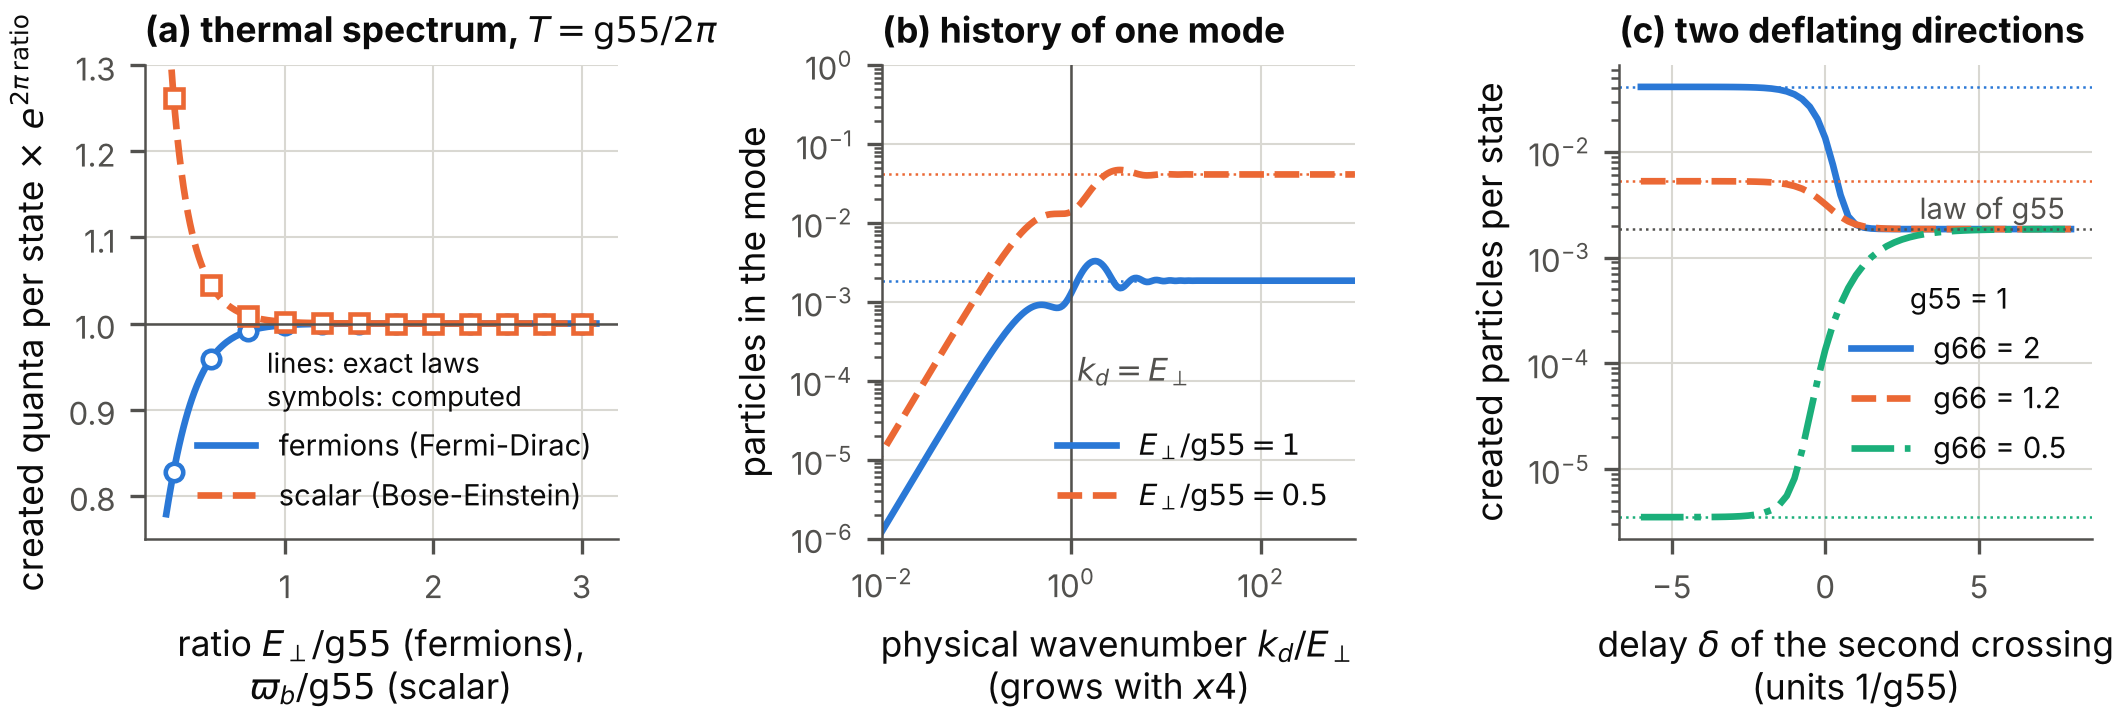
\includegraphics[width=1\textwidth,height=\textheight]{figures/fig_creation.png}
\caption{Creation of particles on the deflating 7+1 spacetime. (a)
Created quanta per state, multiplied by \(e^{2\pi\,\mathrm{ratio}}\),
against the ratio of the energy to the rate. Fermions follow the
Fermi--Dirac law (7.3). For comparison the panel also shows the quanta
of a scalar field on the same spacetime, which follow the Bose--Einstein
law, Eq. (7.3) with \(-1\) in place of \(+1\) and with the energy of the
scalar mode, at the same temperature. Lines: the exact laws; symbols:
computed. (b) History of two modes, with \(E_\perp/\mathrm{g55}=1\) and
\(0.5\): the number of particles in the mode against the physical
wavenumber \(k_d/E_\perp\), which grows with the time. After the
crossing at \(k_d=E_\perp\) the number settles at the value of Eq. (7.3)
(dotted). (c) Two deflating directions, \(\mathrm{g55}=1\) and
\(\mathrm{g66}=2\), \(1.2\) or \(0.5\): mean number of created particles
per state against the delay between the two crossings; the dotted lines
are Eq. (7.3) with each of the two rates.}
\end{figure}

\emph{Meaning.} Each mode with \(k_t\neq0\) is populated once, at its
crossing. Its particles then gain energy without bound, as
\((E_\perp^2+k_d^2)^{1/2}\), like the classical particle of Section 1.7.
Modes with \(k_t=0\) stay empty. The stress of the created particles
must eventually change the metric; that reaction has not been computed,
and the results hold for as long as it can be neglected. The
instantaneous energy of a quantum in a mode with \(k_t\neq0\) is at
least \(|k_t|/b_t\), which grows as \(e^{\mathrm{rate}_t\,x4}\): if the
deflating coordinates are periodic, the smallest wavenumber that differs
from zero is fixed, and the sector of fields that do not depend on
\(x5,x6,x7\) is separated from the rest by a gap that grows
exponentially.

\hypertarget{the-44-spacetime-the-deflation-extinguishes-the-modes-that-depend-on-the-additional-times}{%
\subsection{7.3 The 4+4 spacetime: the deflation extinguishes the modes
that depend on the additional
times}\label{the-44-spacetime-the-deflation-extinguishes-the-modes-that-depend-on-the-additional-times}}

\emph{Exact solution.} In \(K=K_\perp+i\,k_d\,\gamma^4\gamma^d\) the
first matrix is anti-Hermitian with \(K_\perp^2=-E_\perp^2\), the matrix
\(i\gamma^4\gamma^d\) is Hermitian with the square one, and the two
anticommute. Let \(w\) be one of the eight eigenvectors of \(K_\perp\)
with the eigenvalue \(+iE_\perp\); then \(i\gamma^4\gamma^dw\) is an
eigenvector with the eigenvalue \(-iE_\perp\) and is orthogonal to
\(w\). The equation is solved by the modified Bessel functions that
decay at large argument, of the orders
\(\tfrac12\mp iE_\perp/\mathrm{rate}_t\). Such a function is written
here with its order as a subscript and with its argument; the letter
\(K\) without subscript and argument is the matrix of Eq. (4.11). With
the recurrence relations of these functions one verifies by substitution
that

\[\hat\psi=\sqrt{u_d}\,\Big[K_{\frac12-iE_\perp/\mathrm{rate}_t}(u_d)\,w
-K_{\frac12+iE_\perp/\mathrm{rate}_t}(u_d)\,i\gamma^4\gamma^dw\Big]\tag{7.5}\]

solves Eq. (4.11) for each of the eight \(w\); the relative residual,
computed with the Bessel functions of an arbitrary-precision library, is
\(2\times10^{-15}\). The other eight solutions are built in the same way
from the modified Bessel functions that \emph{grow} as \(e^{+u_d}\).

\emph{Standing waves and their extinction.} Since \(u_d\) itself grows
exponentially with the time, a solution of the second kind grows as the
exponential of an exponential. Such a solution is not admissible; it is
the counterpart of the growing exponential under a potential barrier.
Admissible are the eight solutions (7.5), which stay bounded. Because
\(w\) and \(i\gamma^4\gamma^dw\) are orthogonal and the two functions in
Eq. (7.5) are complex conjugates of each other,

\[|\hat\psi|^2=2\,u_d\,\big|K_{\frac12+iE_\perp/\mathrm{rate}_t}(u_d)\big|^2\,|w|^2.\tag{7.6}\]

At early times, \(u_d\to0\),
\(|\hat\psi|^2\to\pi\,|w|^2/\cosh(\pi E_\perp/\mathrm{rate}_t)\), a
constant: the solution is a combination of \(e^{+iE_\perp x4}\,w\) and
\(e^{-iE_\perp x4}\,i\gamma^4\gamma^dw\) with coefficients of
\emph{equal} magnitude. A bounded solution is a \textbf{standing wave}
in the ordinary time, not a traveling wave, and its conserved charge
\(\hat\psi^\dagger W_{1644}\hat\psi\) vanishes. At late times,
\(u_d\to\infty\), \(|\hat\psi|^2\to\pi\,|w|^2\,e^{-2u_d}\): the mode
dies out as the exponential of an exponential of the time.

\emph{The law of the extinction.} In the semiclassical (WKB)
approximation the bounded solution falls beyond the turning value, at
which \(k_d=E_\perp\), as \(e^{-S_{\rm WKB}}\) with

\[S_{\rm WKB}=\int_{x4_{\rm turn}}^{x4}\sqrt{k_d^2-E_\perp^2}\;dx4'
=\frac{1}{\mathrm{rate}_t}\Big[\sqrt{k_d^2-E_\perp^2}-E_\perp\arccos\frac{E_\perp}{k_d}\Big],\tag{7.7}\]

which approaches \((k_d-\tfrac{\pi}{2}E_\perp)/\mathrm{rate}_t\) for
\(k_d\gg E_\perp\). The exact solution fixes the constant that the
approximation leaves open:

\[\ln\frac{|\hat\psi|_{\rm early}}{|\hat\psi|_{\rm late}}-S_{\rm WKB}\ \longrightarrow\
\tfrac12\ln2-\tfrac12\ln\big(1+e^{-2\pi E_\perp/\mathrm{rate}_t}\big).\tag{7.8}\]

\emph{Numerical confirmation} (checks \texttt{44d-M1} to
\texttt{44d-M4}). Beyond the turning value exactly eight of the sixteen
solutions stay bounded; followed backwards to early times they contain
parts of positive and of negative frequency of equal weight, to
\(2\times10^{-14}\). Where one rate governs, the computed magnitude
equals Eq. (7.6) over the range \(0.02<u_d<12\) to a relative deviation
of \(3.6\times10^{-12}\), and Eq. (7.8) holds to \(3.6\times10^{-4}\) at
\(S_{\rm WKB}=30\). With three unequal rates no exact solution is known;
the bounded solutions fall as \(e^{-S_{\rm WKB}}\) times a factor that
depends on the internal state, with a spread of 0.40 in its logarithm at
\(S_{\rm WKB}=30\).

\begin{figure}
\centering
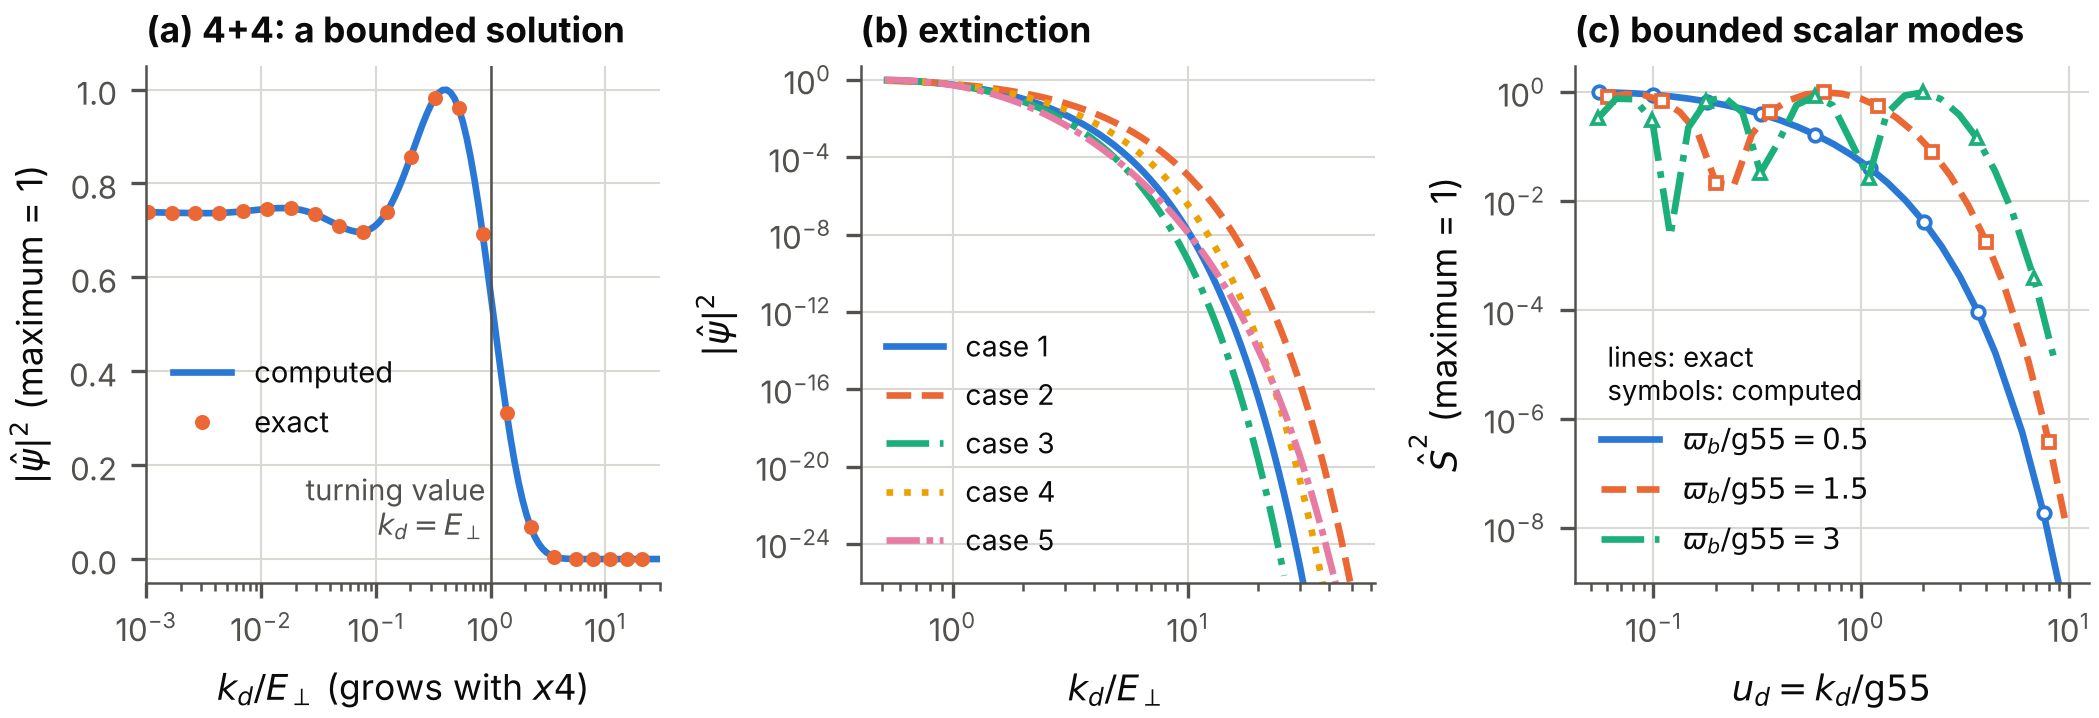
\includegraphics[width=1\textwidth,height=\textheight]{figures/fig_extinction.png}
\caption{Extinction on the deflating 4+4 spacetime. (a) A bounded
solution: \(\lvert\hat\psi\rvert^2\) against the physical wavenumber
\(k_d/E_\perp\), which grows with the time; computed (line) and the
exact form (7.6) (symbols). It is constant long before the crossing at
\(k_d=E_\perp\) and falls after it. (b) Five cases, with one, two or
three wavenumbers \(k_t\) different from zero and with equal and unequal
rates, on a logarithmic scale. (c) The bounded modes of a scalar field
on the same spacetime, which are extinguished in the same way; lines:
exact, symbols: computed.}
\end{figure}

\emph{Meaning.} On the flat 4+4 spacetime a field that depends on the
additional times evolves non-unitarily in the ordinary time; this is the
principal difficulty of four time-like dimensions, and on flat spacetime
it can only be met by imposing that the fields do not depend on those
times. On the deflating 4+4 spacetime every admissible mode that depends
on a deflating time is a standing wave that is extinguished after its
crossing. What remains at late times is the sector of fields that do not
depend on \(x5,x6,x7\), in which the evolution is unitary: the quantized
sector of Part 5. \emph{The deflation of the three additional times
removes, dynamically, the sector that causes the difficulty.} The limits
of this conclusion: the eight growing solutions are discarded because
they are unbounded, which is a condition of admissibility and is not
derived from a principle; and the theory still has no positive conserved
charge for modes that depend on the deflating times.

\hypertarget{the-numerical-method}{%
\subsection{7.4 The numerical method}\label{the-numerical-method}}

The equations of this part are linear, with coefficients that grow
exponentially, and an integrator with a fixed step fails on them. The
program uses a commutator-free Magnus method of the fourth order: over
each step the solution is advanced by the product of two matrix
exponentials of linear combinations of the coefficient matrix at two
Gauss points. Because the square of \(\mathsf h\) or of \(K\) is a
multiple of the unit matrix at any one time, each exponential is
evaluated in closed form; on 7+1 every step is exactly unitary. The
length of a step is chosen so that neither the phase accumulated in it
nor the relative change of the coefficients exceeds a fixed bound. On
7+1 the number of particles is read off by projection on the eigenstates
of the Hamiltonian corrected to the first order in the rate at which its
direction changes, which removes the leading spurious oscillation of the
particle number at finite time. The independent script, which uses an
explicit Runge--Kutta method of the eighth order and the Bessel
functions of another library, reproduces Eq. (7.3) to
\(2.2\times10^{-5}\) and confirms Eq. (7.5) and, to the accuracy of the
semiclassical form at the exponent that it reaches, Eq. (7.8).

\begin{center}\rule{0.5\linewidth}{0.5pt}\end{center}

\hypertarget{part-8.-which-symmetries-survive-the-deflation}{%
\section{Part 8. Which symmetries survive the
deflation}\label{part-8.-which-symmetries-survive-the-deflation}}

\textbf{Rotations and boosts.} The flat spacetimes have 28 rotations and
boosts, one for each pair of coordinates. On the deflating spacetime
(checks \texttt{44d-S1}, \texttt{71d-S1}; table of Section 1.5):

\begin{itemize}
\tightlist
\item
  the six rotations of \(x0,x1,x2,x3\) survive for any rates;
\item
  the rotation of two deflating coordinates survives if and only if
  their rates are equal;
\item
  nothing that involves \(x4\) survives; on 7+1 these are the seven
  boosts, among them the three boosts of special relativity along
  \(x1,x2,x3\);
\item
  nothing that mixes a flat coordinate with a deflating coordinate
  survives.
\end{itemize}

For fields that do not depend on \(x5,x6,x7\) the flat equations hold
for the weighted field (Section 4.3), and their solutions are related by
the ordinary boosts as on flat spacetime. What singles out the preferred
state of rest for such fields is only the dependence of the couplings
(4.6) on the time.

\textbf{The internal symmetry of fields in ordinary space.} For a field
that depends on \(x1,x2,x3,x4\) only, the linear equation of the
weighted field contains four matrices: \(\alpha^1,\alpha^2,\alpha^3\)
and \(\beta\). The matrices that commute with all four generate
transformations of the sixteen components that leave the equation
unchanged: an \textbf{internal symmetry}. Its algebra has the dimension
8 and the structure \(su(2)_A\oplus su(2)_B\oplus u(1)_F\oplus u(1)_E\),
on both spacetimes (check \texttt{def-S3}):

\begin{itemize}
\tightlist
\item
  six generators are the products \(\gamma^a\gamma^b\) of the six pairs
  \(a<b\) taken from the four axes \(x0,x5,x6,x7\); they form the two
  \(su(2)\);
\item
  \(u(1)_F\) is the phase symmetry of Section 4.5 (fermion number);
\item
  \(u(1)_E\) is a second phase symmetry, generated by a traceless
  Hermitian matrix \(P\) with \(P^2=1\), proportional to
  \(\gamma^0\gamma^5\gamma^6\gamma^7\); it distinguishes the states that
  are doublets of \(su(2)_A\) from those that are doublets of
  \(su(2)_B\): at a given momentum the eight states of positive energy
  are four with \(P=+1\), which are doublets of one \(su(2)\) and do not
  transform under the other, and four with \(P=-1\), for which the two
  algebras exchange their roles.
\end{itemize}

Because the weighted field of this sector obeys the flat equations, this
symmetry is not changed by the deflation. But on flat spacetime the six
products \(\gamma^a\gamma^b\) are rotations of the four extra axes,
symmetries of the spacetime; on the deflating spacetime 0, 1 or 3 of
them are still symmetries of the spacetime, for three different, two
equal or three equal rates (checks \texttt{44d-S2}, \texttt{71d-S2};
last three columns of the table of Section 1.5). The others remain exact
symmetries of the sector \emph{without} being symmetries of the
spacetime. On 7+1 the self-interaction respects the six rotations and
\(u(1)_F\) for all couplings, and \(u(1)_E\) only for
\(g_1^{\rm eff}=g_7^{\rm eff}=0\). On 4+4, in form C (the definition),
every self-interaction that does not vanish breaks the three generators
that mix \(x0\) with \(x5,x6,x7\) and breaks \(u(1)_E\); it keeps the
three rotations of \(x5,x6,x7\) among themselves and \(u(1)_F\). In form
Q the 4+4 model behaves as the 7+1 model (Section 6.5).

\textbf{Discrete symmetries.} The scale factors are real and depend on
\(x4\) only. Reflections of any coordinate other than \(x4\), and charge
conjugation on 7+1 (Section 4.5), survive. The reversal of the ordinary
time does not: it turns deflation into inflation.

\begin{center}\rule{0.5\linewidth}{0.5pt}\end{center}

\hypertarget{part-9.-what-has-been-established-and-what-has-not}{%
\section{Part 9. What has been established, and what has
not}\label{part-9.-what-has-been-established-and-what-has-not}}

\textbf{Established} (each item with the checks named in the text; exact
unless marked numerical there):

\begin{enumerate}
\def\labelenumi{\arabic{enumi}.}
\tightlist
\item
  The geometry of the two deflating spacetimes: Christoffel symbols,
  curvature, Einstein tensor, the 14 to 20 Killing vectors; the
  spacetimes are not vacuum solutions of Einstein's equations; with
  equal rates they solve Einstein--Gauss--Bonnet gravity for
  \(\Lambda_8=3\,\mathrm{g55}^2\),
  \(\alpha_{\rm GB}=-1/(4\,\mathrm{g55}^2)\), and that solution is
  unstable (numerical).
\item
  The spin connection
  \(\Omega_t=\tfrac12\mathrm{rate}_t\,b_t\,\gamma^t\gamma^4\), the same
  formula on both spacetimes, and
  \(\gamma^\mu\Omega_\mu=-\tfrac12\mathrm{gsum}\,\gamma^4\).
\item
  The Lagrangians with kinetic term, mass term and self-interaction,
  Eqs. (3.2), (3.5), (3.6), (3.8), and on 4+4 the positive Lagrangian
  (5.3) with the two forms (5.5) and (5.9) of the self-interaction;
  every bilinear in them is real, and every invariant \(I_r\) is
  invariant under the transformations of the frame.
\item
  The field equations (4.1) and (4.2), and their forms (4.3), (4.4),
  (4.7), (4.8), (5.6), (5.10), (5.13).
\item
  The weighted field obeys the flat equations with every quartic
  coupling divided by \(V_d\) and with the mass unchanged.
\item
  Of the nine couplings only four combinations are independent, Eq.
  (6.5). Uniform matter on 7+1 feels the two Hartree--Fock couplings
  (6.7); on 4+4 it feels four couplings (6.9), the same four
  combinations in both forms with the roles of the total densities and
  of the differences between the halves exchanged. The pair couplings of
  the 28 pairs at rest, Eq. (6.14) and the table of Section 6.4. The
  conditions for chiral symmetry (6.16) and for the internal symmetry of
  fields in ordinary space; in particular, every self-interaction of
  form C breaks \(SO(4)\times U(1)_E\) to \(SO(3)_T\).
\item
  On 4+4 the covariant Lagrangian is indefinite, Eq. (5.1); form C of
  the self-interaction is form Q with \(W_{1644}\) inserted in every
  bilinear, Eqs. (5.11) and (5.12): two particles of the same half of
  the field interact identically in the two forms, a particle of each
  half with opposite signs.
\item
  Numerically, in the mean-field approximation of Section 6.6 and for
  the sets A and B of couplings: matter of form C is polarized and binds
  with one half of the field filled, at two to three times the strength
  at which matter of form Q binds with both halves equally filled; a
  massless field acquires in vacuum masses of opposite sign in the two
  halves in form C and of equal sign in form Q, at the same critical
  strength.
\item
  The exact solutions (7.2) and (7.5) of the linear equations when one
  rate governs; the law of creation (7.3) on 7+1; the extinction (7.6)
  to (7.8) on 4+4 (confirmed numerically).
\end{enumerate}

\textbf{Not established:}

\begin{enumerate}
\def\labelenumi{\arabic{enumi}.}
\tightlist
\item
  \emph{What sustains the deflation.} The metric is a hypothesis. It is
  not a solution of Einstein's equations without matter, and the one
  theory in which it is a vacuum solution does not hold it stable.
\item
  \emph{Which form of the self-interaction is the right one for the 4+4
  model} (Sections 5.6 and 6.7). Form C is the definition, by the
  author's decision; form Q gives different interactions between the two
  halves of the field, and nothing in the calculations decides between
  them. 2a. \emph{States with coherence between the two halves, and
  other couplings.} The density matrix (6.8) is diagonal in
  \(W_{1644}\). Because the interaction connects the halves, states with
  \(\langle\psi_+^\dagger\cdots\psi_-\rangle\neq0\) are possible in
  principle in both forms; whether one of them has a lower energy than
  the states of Section 6.6 has not been examined. The numbers of
  Section 6.6 are for the sets A and B; the exact formulas hold for all
  couplings.
\item
  \emph{The values of the couplings \(g_r\) and of the mass \(m\).}
  Nothing in this document fixes them.
\item
  \emph{Solutions of the nonlinear equations.} Part 7 solves the linear
  equations. With the self-interaction the field equations are solved in
  the project only in mean-field approximations for uniform matter and
  for pairs; an exact solution is not known.
\item
  \emph{Modes with unequal rates and several \(k_t\neq0\)} are known
  only numerically.
\item
  \emph{The reaction of the created particles on the metric} (7+1), and
  \emph{a principle that excludes the growing solutions} (4+4).
\end{enumerate}

\begin{center}\rule{0.5\linewidth}{0.5pt}\end{center}

\hypertarget{appendix-a.-complete-output-of-the-programs}{%
\section{Appendix A. Complete output of the
programs}\label{appendix-a.-complete-output-of-the-programs}}

The reports are printed as the programs wrote them (a line that is too
long to be typeset is continued on the following lines, broken at
spaces). In them the rates are called \texttt{g55}, \texttt{g66},
\texttt{g77}; \texttt{rate\_t}, \texttt{b\_t}, \texttt{const5} and so on
are the quantities of the same names in the text;
\texttt{gamma1644{[}A{]}} and \texttt{gamma1671{[}A{]}} are the matrices
\(\gamma_{1644}^A\) and \(\gamma_{1671}^A\); \texttt{Cm1644} is
\(C^-_{1644}\); \texttt{psihat} is the weighted field \(\hat\psi\);
\texttt{gs} is the list of the signs \(\mathrm{gs}_{AA}\) and \texttt{c}
the constant \(c_\gamma\) of Section 0.2; \texttt{G\_0} and
\texttt{G\_1} are \(G_S^{\rm HF}\) and \(G_V^{\rm HF}\), \texttt{G\_S0}
and \texttt{G\_V0} (also written \texttt{G\_Sc}, \texttt{G\_Vc}) are
\(G_S^{\rm c}\) and \(G_V^{\rm c}\); \texttt{G\_Stot}, \texttt{G\_Vtot},
\texttt{G\_Sdif}, \texttt{G\_Vdif}, \texttt{G\_Ssame},
\texttt{G\_Vsame}, \texttt{G\_Sopp}, \texttt{G\_Vopp} are the couplings
of Eqs. (6.9) and (6.11); \texttt{eps\_K} is \(\mathrm{sgn}_K\);
\texttt{F} is the Fierz matrix \(\mathsf F\); \texttt{rho} and
\texttt{rho\_S} (in the report of the command \texttt{forms}: \texttt{n}
and \texttt{n\_S}) are the densities \(n\) and \(n_S\), \texttt{s\_+-}
the scalar densities \(n_{S\pm}\); \texttt{M}, \texttt{M\_+},
\texttt{M\_-} are the masses \(m^*\), \(m^*_+\), \(m^*_-\); \texttt{W}
is \(W_{1644}\); ``the covariant form'' is form C and ``the
quantized-sector form'' is form Q. ``The main project'' means the part
of PROJECT spacetimes that treats the flat 4+4 and 7+1 spacetimes: its
program is used as a library, the matrices of the frame are its
matrices, and several checks compare with its data files. ``The author's
document'' means his document on Kohn--Sham matter and gravity on the
7+1 spacetime.

\hypertarget{a.1-geometry-coordinate-matrices-spin-connection-dirac-operators-deflation_cjt_ks_c-matrices}{%
\subsection{\texorpdfstring{A.1 Geometry, coordinate matrices, spin
connection, Dirac operators
(\texttt{deflation\_cjt\_ks\_c\ matrices})}{A.1 Geometry, coordinate matrices, spin connection, Dirac operators (deflation\_cjt\_ks\_c matrices)}}\label{a.1-geometry-coordinate-matrices-spin-connection-dirac-operators-deflation_cjt_ks_c-matrices}}

\begin{Shaded}
\begin{Highlighting}[]
\NormalTok{PROJECT spacetimes, Revision\_Deflation\_CJT\_and\_Kohn{-}Sham\_definition\_C: checks of the geometry, of the Dirac matrices, of the spin connection and of the Dirac operators of the deflating spacetimes (44d{-}..: 4+4 with deflating x5, x6, x7; 71d{-}..: 7+1 with deflating x5, x6, x7)}
\NormalTok{generated by: deflation\_cjt\_ks\_c (Rust crate spacetimes{-}deflation{-}cjt{-}ks{-}c, version 0.1.0; PROJECT spacetimes, Revision\_Deflation\_CJT\_and\_Kohn{-}Sham\_definition\_C); command: deflation\_cjt\_ks\_c matrices}
\NormalTok{47 of 47 checks passed}

\NormalTok{[PASS] 44d{-}G1  (exact) metric of the deflating 4+4 spacetime in the author\textquotesingle{}s sign convention (space{-}like +, time{-}like {-}): g = diag(gs\_00, .., gs\_44, gs\_55 b\_5\^{}2, gs\_66 b\_6\^{}2, gs\_77 b\_7\^{}2) with the metric signs gs = diag[1, 1, 1, 1, {-}1, {-}1, {-}1, {-}1] and the scale factors b\_5 = const5 exp({-}g55 x4), b\_6 = const6 exp({-}g66 x4), b\_7 = const7 exp({-}g77 x4), that is g\_55 = {-}const5\^{}2 exp({-}2 g55 x4) and likewise g\_66, g\_77 (the author\textquotesingle{}s formulas for this spacetime, on which x5, x6, x7 are time{-}like; g55, g66, g77 \textgreater{} 0 are the three rates, and in statements with a general index t = 5, 6, 7 the rate of xt is written rate\_t, gsum = g55 + g66 + g77). Verified: g\_tt = {-}b\_t\^{}2 and d g\_tt/dx4 = {-}2 rate\_t g\_tt; the frame e\^{}A = (dx0, .., dx4, b\_5 dx5, b\_6 dx6, b\_7 dx7) is orthonormal. All exact geometry checks use five rational parameter sets: (g55, g66, g77) = (1, 1, 1) at a point where (b\_5, b\_6, b\_7) = (1, 1, 1); (g55, g66, g77) = (1, 2, 3) at a point where (b\_5, b\_6, b\_7) = (1/2, 1/3, 1/5); (g55, g66, g77) = (1/2, 3/4, 5/3) at a point where (b\_5, b\_6, b\_7) = (2, 1/3, 5/7); (g55, g66, g77) = (2, 2, 5) at a point where (b\_5, b\_6, b\_7) = (3/2, 3/2, 1/4); (g55, g66, g77) = (7/3, 7/3, 7/3) at a point where (b\_5, b\_6, b\_7) = (1/2, 3, 5/4)}
\NormalTok{[PASS] 44d{-}G2  (exact) the Christoffel symbols computed from their definition are Gamma\^{}t\_(4t) = Gamma\^{}t\_(t4) = {-}rate\_t and Gamma\^{}4\_(tt) = {-}gs\_tt rate\_t b\_t\^{}2 = + rate\_t b\_t\^{}2 (t = 5, 6, 7); all others vanish}
\NormalTok{[PASS] 44d{-}G3  (exact) Cartan\textquotesingle{}s structure equations hold with the spin{-}connection coefficients of the tetrad postulate: the torsion d e\^{}A + omega\^{}A\_B \^{} e\^{}B vanishes, and d omega\^{}A\_B + omega\^{}A\_C \^{} omega\^{}C\_B equals the Riemann tensor computed from the Christoffel symbols (two independent routes to the curvature)}
\NormalTok{[PASS] 44d{-}G4  (exact) Riemann tensor in the orthonormal frame: R\^{}t\_(4t4) = {-}rate\_t\^{}2, R\^{}4\_(t4t) = gs\_tt rate\_t\^{}2 = {-}rate\_t\^{}2, R\^{}t\_(sts) = gs\_ss rate\_t rate\_s = {-}rate\_t rate\_s (t != s in \{5, 6, 7\}), and the components that follow from antisymmetry; all other components vanish. No component involves x0, x1, x2 or x3: the four space coordinates x0, x1, x2, x3 stay flat}
\NormalTok{[PASS] 44d{-}G5  (exact) with gsq = g55\^{}2 + g66\^{}2 + g77\^{}2 and gsum = g55 + g66 + g77, in the author\textquotesingle{}s sign convention of the metric: Ricci tensor R\^{}4\_4 = gsq, R\^{}t\_t = rate\_t gsum, R\^{}a\_a = 0 (a = 0..3); curvature scalar R = gsq + gsum\^{}2; Einstein tensor G\^{}4\_4 = {-}(g55 g66 + g55 g77 + g66 g77), G\^{}t\_t = rate\_t gsum {-} (gsq + gsum\^{}2)/2, G\^{}a\_a = {-}(gsq + gsum\^{}2)/2; all are constants (they do not depend on x4), the mixed components are the same on the 4+4 and on the 7+1 spacetime, and the covariant divergence of the Einstein tensor vanishes (contracted Bianchi identity)}
\NormalTok{[PASS] 44d{-}G6  (exact) Killing vectors (the Lie derivative of the metric along each vanishes identically): 7 translations (x0, x1, x2, x3, x5, x6, x7), 6 rotations of (x0, x1, x2, x3), and the scaling d/dx4 + sum\_t rate\_t xt d/dxt, 14 in all; one more for every pair of equal rates (a rotation of the two coordinates), and three more if all three rates are equal (20 in all). Numbers found for the five parameter sets: [20, 14, 14, 15, 20]}
\NormalTok{[PASS] 44d{-}G7  (exact) if the three rates are equal, g55 = g66 = g77, the part (x4, x5, x6, x7) of the metric has constant curvature, R\_(rho sigma mu nu) = +g55\^{}2 (g\_(rho mu) g\_(sigma nu) {-} g\_(rho nu) g\_(sigma mu)): the four time{-}like coordinates carry minus the metric of hyperbolic space H\^{}4 of radius 1/g55, written in horospherical coordinates (the upper{-}half{-}space form)}
\NormalTok{[PASS] 44d{-}G10  (exact) Lovelock gravity, in the author\textquotesingle{}s sign convention of the metric (space{-}like components positive), with the action R {-} 2 Lambda\_8 + alpha\_GB (R\^{}2 {-} 4 R\_(mu nu) R\^{}(mu nu) + R\_(mu nu rho sigma) R\^{}(mu nu rho sigma)) and the field equations G\^{}mu\_nu + Lambda\_8 delta\^{}mu\_nu + alpha\_GB Lanczos\^{}mu\_nu = 0: the curvature acts diagonally on pairs of frame directions; the Lanczos tensor of the Gauss{-}Bonnet term is Lanczos\^{}a\_a = {-}4 g55 g66 g77 gsum (a = 0..3), Lanczos\^{}4\_4 = Lanczos\^{}t\_t = 0; the Lovelock tensor of third order vanishes identically. For three equal rates (2 of the five parameter sets) the deflating spacetime solves the vacuum field equations with Lambda\_8 = 3 g55\^{}2 and alpha\_GB = {-}1/(4 g55\^{}2), that is 4 alpha\_GB Lambda\_8 = {-}3: the deflation needs no matter as its source in Einstein{-}Gauss{-}Bonnet gravity. For rates that are not all equal no choice of Lambda\_8 and alpha\_GB satisfies the components 4, 5, 6, 7}
\NormalTok{[PASS] 44d{-}G9  (numerical) geodesic with m = 1, momentum P\_1 = 0.5 along x1 and P\_5 = 0.3 along the deflating time x5 (g55 = 1, const5 = 0.8), started at x4 = {-}2 with increasing x4: P\_1, P\_5 and the norm are conserved to 1.7e{-}14; the path reaches the largest value x4 = 1.09240103 (predicted turning value ln(E\_perp const5/|P\_5|)/g55 with E\_perp = sqrt(m\^{}2 + P\_1\^{}2) = 1.09240103) after the affine parameter 3.38543615 (closed form 3.38543615) and then returns to smaller x4: a particle with momentum along a deflating time cannot pass the turning value}
\NormalTok{[PASS] 44d{-}C1  (exact) the coordinate matrices gamma\^{}mu = e\_A\^{}mu gamma1644[A] of the deflating 4+4 spacetime (gamma\^{}t = gamma1644[t]/b\_t for t = 5, 6, 7; the other five unchanged) are real and satisfy gamma\^{}mu.gamma\^{}nu + gamma\^{}nu.gamma\^{}mu = 2 c g\^{}(mu nu) 1 for all 64 pairs, with c = +1 and the inverse metric g\^{}(mu nu) of the author\textquotesingle{}s sign convention (space{-}like +, time{-}like {-}; g\^{}(tt) = {-}1/b\_t\^{}2). The squares of the matrices are therefore equal to the signs of the metric. Verified for five rational parameter sets: (g55, g66, g77) = (1, 1, 1) at a point where (b\_5, b\_6, b\_7) = (1, 1, 1); (g55, g66, g77) = (1, 2, 3) at a point where (b\_5, b\_6, b\_7) = (1/2, 1/3, 1/5); (g55, g66, g77) = (1/2, 3/4, 5/3) at a point where (b\_5, b\_6, b\_7) = (2, 1/3, 5/7); (g55, g66, g77) = (2, 2, 5) at a point where (b\_5, b\_6, b\_7) = (3/2, 3/2, 1/4); (g55, g66, g77) = (7/3, 7/3, 7/3) at a point where (b\_5, b\_6, b\_7) = (1/2, 3, 5/4)}
\NormalTok{[PASS] 44d{-}C2  (exact) the spin{-}connection coefficients computed from the tetrad postulate omega\_mu\^{}A\_B = e\^{}A\_nu (d\_mu e\_B\^{}nu + Gamma\^{}nu\_(mu lam) e\_B\^{}lam), with the Christoffel symbols obtained from the metric, and with the first frame index lowered by the metric signs gs, omega\_(mu A B) = gs\_AA omega\_mu\^{}A\_B, are antisymmetric, omega\_(mu A B) = {-}omega\_(mu B A), and the only non{-}zero ones are omega\_(t,t4) = {-}omega\_(t,4t) = {-}gs\_tt rate\_t b\_t = + rate\_t b\_t (t = 5, 6, 7); same five parameter sets}
\NormalTok{[PASS] 44d{-}C3  (exact) Omega\_mu := (c/4) omega\_(mu A B) gamma1644[A].gamma1644[B] with c = +1 equals +(1/2) rate\_t b\_t gamma1644[t].gamma1644[4] for mu = t in \{5, 6, 7\} and vanishes for mu = 0..4 (the same formula on both spacetimes, because c gs\_tt = {-}1 on both): the spin connection is an element of the Lie algebra spanned by the scaled commutators Sigma\^{}(t4)}
\NormalTok{[PASS] 44d{-}C4  (exact) d\_mu gamma\^{}nu + Gamma\^{}nu\_(mu lam) gamma\^{}lam + [Omega\_mu, gamma\^{}nu] = 0 for all 64 pairs (mu, nu), with d\_4 gamma\^{}t = +rate\_t gamma\^{}t: the coordinate matrices are covariantly constant}
\NormalTok{[PASS] 44d{-}C5  (exact) sum\_mu gamma\^{}mu.Omega\_mu = {-}(1/2) (g55 + g66 + g77) gamma1644[4]: in the Dirac operator the spin connection amounts to the replacement d\_4 {-}\textgreater{} d\_4 {-} gsum/2, which the weighted field psihat = sqrt(b\_5 b\_6 b\_7) psi removes}
\NormalTok{[PASS] 44d{-}C6  (exact) d\_mu Omega\_nu {-} d\_nu Omega\_mu + [Omega\_mu, Omega\_nu] = (c/4) R\_(A B mu nu) gamma1644[A].gamma1644[B] for all 64 pairs (mu, nu), with c = +1 and with the Riemann tensor that metric.rs computes from the metric, its first index lowered by the metric (d\_4 Omega\_t = {-}rate\_t Omega\_t): the curvature of the spinor derivative is the Riemann tensor}
\NormalTok{[PASS] 44d{-}C7  (exact) (1/2) sum\_(mu nu) gamma\^{}mu.gamma\^{}nu.(d\_mu Omega\_nu {-} d\_nu Omega\_mu + [Omega\_mu, Omega\_nu]) = {-}(c R/4) 1 = {-} (R/4) 1 with the curvature scalar R = g55\^{}2 + g66\^{}2 + g77\^{}2 + gsum\^{}2 of the author\textquotesingle{}s sign convention: the square of the Dirac operator differs from c times the wave operator of the spinor derivative by this term}
\NormalTok{[PASS] 44d{-}C8  (exact) transpose(Omega\_mu).Cm1644 + Cm1644.Omega\_mu = 0 (Cm1644 = gamma1644[0].gamma1644[1].gamma1644[2].gamma1644[3]): the adjoint field psi\^{}dagger Cm1644 is differentiated with {-}Omega\_mu on its right, as the conserved current requires}
\NormalTok{[PASS] 44d{-}D1  (exact) in momentum space (d\_mu {-}\textgreater{} i k\_mu) the Dirac operator of the weighted field at fixed x4, D = i gamma\^{}mu k\_mu with the coordinate matrices, satisfies (D + m)(D {-} m) = {-}(g\^{}(mu nu) k\_mu k\_nu + m\^{}2) 1 with g\^{}(mu nu) k\_mu k\_nu = k\_0\^{}2 + k\_1\^{}2 + k\_2\^{}2 + k\_3\^{}2 {-} k\_4\^{}2 {-} sum\_t k\_t\^{}2/b\_t\^{}2: the instantaneous mass shell is k\_4\^{}2 + sum\_t k\_t\^{}2/b\_t(x4)\^{}2 = |k|\^{}2 + m\^{}2. Verified for five rational parameter sets and four rational momenta each}
\NormalTok{[PASS] 44d{-}D2  (exact) the generator of the evolution of the weighted field in x4, K(x4) = {-}m gamma1644[4] + i sum\_a k\_a gamma1644[4].gamma1644[a] + i sum\_t (k\_t/b\_t(x4)) gamma1644[4].gamma1644[t], satisfies K\^{}2 = (sum\_t k\_t\^{}2/b\_t\^{}2 {-} m\^{}2 {-} |k|\^{}2) 1 and K + K\^{}dagger = 2 i sum\_t (k\_t/b\_t) gamma1644[4].gamma1644[t]}
\NormalTok{[PASS] 44d{-}D3  (exact) dK/dx4 = i sum\_t rate\_t (k\_t/b\_t) gamma1644[4].gamma1644[t] is a Hermitian matrix whose square is sum\_t (rate\_t k\_t/b\_t)\^{}2 times the unit matrix; the weighted field obeys the second{-}order equation d\_4\^{}2 psihat = (K\^{}2 + dK/dx4) psihat, a Klein{-}Gordon equation with a term that depends on the spin}
\NormalTok{[PASS] 44d{-}D4  (exact) W = i Cm1644.gamma1644[4] is Hermitian with W\^{}2 = 1 and trace 0, and W.K + K\^{}dagger.W = 0 for every momentum and all k\_5, k\_6, k\_7: the covariant charge psihat\^{}dagger W psihat of a mode is conserved on the deflating spacetime, and it is not positive}
\NormalTok{[PASS] 44d{-}D5  (exact) K is anti{-}Hermitian (the evolution in x4 is unitary and psihat\^{}dagger psihat is conserved) if and only if k\_5 = k\_6 = k\_7 = 0, that is, if the field does not depend on the deflating times}
\NormalTok{[PASS] 44d{-}D6  (exact) with gamma1644[A] = [[0, taubar1644[A]], [tau1644[A], 0]] the operator gamma\^{}mu d\_mu of the weighted field has the blocks [[0, sum\_A taubar1644[A] e\_A\^{}mu d\_mu], [sum\_A tau1644[A] e\_A\^{}mu d\_mu, 0]], e\_A\^{}mu d\_mu = (d\_0, .., d\_4, d\_5/b\_5, d\_6/b\_6, d\_7/b\_7): the equation is the pair taubar\^{}A e\_A\^{}mu d\_mu psihat\^{}R = m psihat\^{}L, tau\^{}A e\_A\^{}mu d\_mu psihat\^{}L = m psihat\^{}R of real 8{-}component equations}
\NormalTok{[PASS] 44d{-}D7  (exact) worked example: m = 3, k = 0, (k\_5, k\_6, k\_7) = (1, 0, 0) at the value of x4 where b\_5 = 1/5 (so k\_5/b\_5 = 5 \textgreater{} m): K\^{}2 = +16 1, and (4 + K)/8 and (4 {-} K)/8 are complementary projectors of trace 8: at this x4 eight independent solutions grow as exp(+4 x4) and eight decay as exp({-}4 x4) to first order. A mode that depends on a deflating time is oscillatory only while k\_t/b\_t(x4) \textless{} sqrt(m\^{}2 + |k|\^{}2)}
\NormalTok{[PASS] 71d{-}G1  (exact) metric of the deflating 7+1 spacetime in the author\textquotesingle{}s sign convention (space{-}like +, time{-}like {-}): g = diag(gs\_00, .., gs\_44, gs\_55 b\_5\^{}2, gs\_66 b\_6\^{}2, gs\_77 b\_7\^{}2) with the metric signs gs = diag[1, 1, 1, 1, {-}1, 1, 1, 1] and the scale factors b\_5 = const5 exp({-}g55 x4), b\_6 = const6 exp({-}g66 x4), b\_7 = const7 exp({-}g77 x4), that is g\_55 = +const5\^{}2 exp({-}2 g55 x4) and likewise g\_66, g\_77 (the author\textquotesingle{}s formulas for this spacetime, on which x5, x6, x7 are space{-}like; g55, g66, g77 \textgreater{} 0 are the three rates, and in statements with a general index t = 5, 6, 7 the rate of xt is written rate\_t, gsum = g55 + g66 + g77). Verified: g\_tt = +b\_t\^{}2 and d g\_tt/dx4 = {-}2 rate\_t g\_tt; the frame e\^{}A = (dx0, .., dx4, b\_5 dx5, b\_6 dx6, b\_7 dx7) is orthonormal. All exact geometry checks use five rational parameter sets: (g55, g66, g77) = (1, 1, 1) at a point where (b\_5, b\_6, b\_7) = (1, 1, 1); (g55, g66, g77) = (1, 2, 3) at a point where (b\_5, b\_6, b\_7) = (1/2, 1/3, 1/5); (g55, g66, g77) = (1/2, 3/4, 5/3) at a point where (b\_5, b\_6, b\_7) = (2, 1/3, 5/7); (g55, g66, g77) = (2, 2, 5) at a point where (b\_5, b\_6, b\_7) = (3/2, 3/2, 1/4); (g55, g66, g77) = (7/3, 7/3, 7/3) at a point where (b\_5, b\_6, b\_7) = (1/2, 3, 5/4)}
\NormalTok{[PASS] 71d{-}G2  (exact) the Christoffel symbols computed from their definition are Gamma\^{}t\_(4t) = Gamma\^{}t\_(t4) = {-}rate\_t and Gamma\^{}4\_(tt) = {-}gs\_tt rate\_t b\_t\^{}2 = {-} rate\_t b\_t\^{}2 (t = 5, 6, 7); all others vanish}
\NormalTok{[PASS] 71d{-}G3  (exact) Cartan\textquotesingle{}s structure equations hold with the spin{-}connection coefficients of the tetrad postulate: the torsion d e\^{}A + omega\^{}A\_B \^{} e\^{}B vanishes, and d omega\^{}A\_B + omega\^{}A\_C \^{} omega\^{}C\_B equals the Riemann tensor computed from the Christoffel symbols (two independent routes to the curvature)}
\NormalTok{[PASS] 71d{-}G4  (exact) Riemann tensor in the orthonormal frame: R\^{}t\_(4t4) = {-}rate\_t\^{}2, R\^{}4\_(t4t) = gs\_tt rate\_t\^{}2 = +rate\_t\^{}2, R\^{}t\_(sts) = gs\_ss rate\_t rate\_s = +rate\_t rate\_s (t != s in \{5, 6, 7\}), and the components that follow from antisymmetry; all other components vanish. No component involves x0, x1, x2 or x3: the four space coordinates x0, x1, x2, x3 stay flat}
\NormalTok{[PASS] 71d{-}G5  (exact) with gsq = g55\^{}2 + g66\^{}2 + g77\^{}2 and gsum = g55 + g66 + g77, in the author\textquotesingle{}s sign convention of the metric: Ricci tensor R\^{}4\_4 = gsq, R\^{}t\_t = rate\_t gsum, R\^{}a\_a = 0 (a = 0..3); curvature scalar R = gsq + gsum\^{}2; Einstein tensor G\^{}4\_4 = {-}(g55 g66 + g55 g77 + g66 g77), G\^{}t\_t = rate\_t gsum {-} (gsq + gsum\^{}2)/2, G\^{}a\_a = {-}(gsq + gsum\^{}2)/2; all are constants (they do not depend on x4), the mixed components are the same on the 4+4 and on the 7+1 spacetime, and the covariant divergence of the Einstein tensor vanishes (contracted Bianchi identity)}
\NormalTok{[PASS] 71d{-}G6  (exact) Killing vectors (the Lie derivative of the metric along each vanishes identically): 7 translations (x0, x1, x2, x3, x5, x6, x7), 6 rotations of (x0, x1, x2, x3), and the scaling d/dx4 + sum\_t rate\_t xt d/dxt, 14 in all; one more for every pair of equal rates (a rotation of the two coordinates), and three more if all three rates are equal (20 in all). Numbers found for the five parameter sets: [20, 14, 14, 15, 20]}
\NormalTok{[PASS] 71d{-}G7  (exact) if the three rates are equal, g55 = g66 = g77, the part (x4, x5, x6, x7) of the metric has constant curvature, R\_(rho sigma mu nu) = +g55\^{}2 (g\_(rho mu) g\_(sigma nu) {-} g\_(rho nu) g\_(sigma mu)) in the author\textquotesingle{}s sign convention: it is de Sitter space of radius 1/g55 in the contracting half of its flat slicing}
\NormalTok{[PASS] 71d{-}G10  (exact) Lovelock gravity, in the author\textquotesingle{}s sign convention of the metric (space{-}like components positive), with the action R {-} 2 Lambda\_8 + alpha\_GB (R\^{}2 {-} 4 R\_(mu nu) R\^{}(mu nu) + R\_(mu nu rho sigma) R\^{}(mu nu rho sigma)) and the field equations G\^{}mu\_nu + Lambda\_8 delta\^{}mu\_nu + alpha\_GB Lanczos\^{}mu\_nu = 0: the curvature acts diagonally on pairs of frame directions; the Lanczos tensor of the Gauss{-}Bonnet term is Lanczos\^{}a\_a = {-}4 g55 g66 g77 gsum (a = 0..3), Lanczos\^{}4\_4 = Lanczos\^{}t\_t = 0; the Lovelock tensor of third order vanishes identically. For three equal rates (2 of the five parameter sets) the deflating spacetime solves the vacuum field equations with Lambda\_8 = 3 g55\^{}2 and alpha\_GB = {-}1/(4 g55\^{}2), that is 4 alpha\_GB Lambda\_8 = {-}3: the deflation needs no matter as its source in Einstein{-}Gauss{-}Bonnet gravity. For rates that are not all equal no choice of Lambda\_8 and alpha\_GB satisfies the components 4, 5, 6, 7}
\NormalTok{[PASS] 71d{-}G8  (numerical) geodesic of a particle of mass m = 1 with momentum P\_1 = 0.5 along x1 and P\_5 = 0.3 along the deflating coordinate x5 (g55 = 1, const5 = 0.8), integrated from x4 = {-}2 to x4 = 4 by the Runge{-}Kutta method: P\_1, P\_5 and the norm are conserved to 2.0e{-}10; the affine parameter (the proper time, since m = 1) that elapses is 3.3375401839, the closed form gives 3.3375401839; the proper time to x4 = infinity is finite, 3.386358: a particle that moves along a deflating coordinate leaves the coordinate patch after a finite proper time, with unbounded energy}
\NormalTok{[PASS] 71d{-}C1  (exact) the coordinate matrices gamma\^{}mu = e\_A\^{}mu gamma1671[A] of the deflating 7+1 spacetime (gamma\^{}t = gamma1671[t]/b\_t for t = 5, 6, 7; the other five unchanged) are real and satisfy gamma\^{}mu.gamma\^{}nu + gamma\^{}nu.gamma\^{}mu = 2 c g\^{}(mu nu) 1 for all 64 pairs, with c = {-}1 and the inverse metric g\^{}(mu nu) of the author\textquotesingle{}s sign convention (space{-}like +, time{-}like {-}; g\^{}(tt) = +1/b\_t\^{}2). The squares of the matrices are therefore opposite to the signs of the metric. Verified for five rational parameter sets: (g55, g66, g77) = (1, 1, 1) at a point where (b\_5, b\_6, b\_7) = (1, 1, 1); (g55, g66, g77) = (1, 2, 3) at a point where (b\_5, b\_6, b\_7) = (1/2, 1/3, 1/5); (g55, g66, g77) = (1/2, 3/4, 5/3) at a point where (b\_5, b\_6, b\_7) = (2, 1/3, 5/7); (g55, g66, g77) = (2, 2, 5) at a point where (b\_5, b\_6, b\_7) = (3/2, 3/2, 1/4); (g55, g66, g77) = (7/3, 7/3, 7/3) at a point where (b\_5, b\_6, b\_7) = (1/2, 3, 5/4)}
\NormalTok{[PASS] 71d{-}C2  (exact) the spin{-}connection coefficients computed from the tetrad postulate omega\_mu\^{}A\_B = e\^{}A\_nu (d\_mu e\_B\^{}nu + Gamma\^{}nu\_(mu lam) e\_B\^{}lam), with the Christoffel symbols obtained from the metric, and with the first frame index lowered by the metric signs gs, omega\_(mu A B) = gs\_AA omega\_mu\^{}A\_B, are antisymmetric, omega\_(mu A B) = {-}omega\_(mu B A), and the only non{-}zero ones are omega\_(t,t4) = {-}omega\_(t,4t) = {-}gs\_tt rate\_t b\_t = {-} rate\_t b\_t (t = 5, 6, 7); same five parameter sets}
\NormalTok{[PASS] 71d{-}C3  (exact) Omega\_mu := (c/4) omega\_(mu A B) gamma1671[A].gamma1671[B] with c = {-}1 equals +(1/2) rate\_t b\_t gamma1671[t].gamma1671[4] for mu = t in \{5, 6, 7\} and vanishes for mu = 0..4 (the same formula on both spacetimes, because c gs\_tt = {-}1 on both): the spin connection is an element of the Lie algebra spanned by the scaled commutators Sigma\^{}(t4)}
\NormalTok{[PASS] 71d{-}C4  (exact) d\_mu gamma\^{}nu + Gamma\^{}nu\_(mu lam) gamma\^{}lam + [Omega\_mu, gamma\^{}nu] = 0 for all 64 pairs (mu, nu), with d\_4 gamma\^{}t = +rate\_t gamma\^{}t: the coordinate matrices are covariantly constant}
\NormalTok{[PASS] 71d{-}C5  (exact) sum\_mu gamma\^{}mu.Omega\_mu = {-}(1/2) (g55 + g66 + g77) gamma1671[4]: in the Dirac operator the spin connection amounts to the replacement d\_4 {-}\textgreater{} d\_4 {-} gsum/2, which the weighted field psihat = sqrt(b\_5 b\_6 b\_7) psi removes}
\NormalTok{[PASS] 71d{-}C6  (exact) d\_mu Omega\_nu {-} d\_nu Omega\_mu + [Omega\_mu, Omega\_nu] = (c/4) R\_(A B mu nu) gamma1671[A].gamma1671[B] for all 64 pairs (mu, nu), with c = {-}1 and with the Riemann tensor that metric.rs computes from the metric, its first index lowered by the metric (d\_4 Omega\_t = {-}rate\_t Omega\_t): the curvature of the spinor derivative is the Riemann tensor}
\NormalTok{[PASS] 71d{-}C7  (exact) (1/2) sum\_(mu nu) gamma\^{}mu.gamma\^{}nu.(d\_mu Omega\_nu {-} d\_nu Omega\_mu + [Omega\_mu, Omega\_nu]) = {-}(c R/4) 1 = + (R/4) 1 with the curvature scalar R = g55\^{}2 + g66\^{}2 + g77\^{}2 + gsum\^{}2 of the author\textquotesingle{}s sign convention: the square of the Dirac operator differs from c times the wave operator of the spinor derivative by this term}
\NormalTok{[PASS] 71d{-}C8  (exact) transpose(Omega\_mu).gamma1671[4] + gamma1671[4].Omega\_mu = 0: the adjoint field psi\^{}dagger gamma1671[4] is differentiated with {-}Omega\_mu on its right, as the conserved current requires}
\NormalTok{[PASS] 71d{-}D1  (exact) in momentum space (d\_mu {-}\textgreater{} {-}i k\_mu) the Dirac operator of the weighted field at fixed x4 is gamma\^{}mu k\_mu {-} m with the coordinate matrices, and (gamma\^{}mu k\_mu + m)(gamma\^{}nu k\_nu {-} m) = {-}(g\^{}(mu nu) k\_mu k\_nu + m\^{}2) 1 with g\^{}(mu nu) k\_mu k\_nu = {-}k\_4\^{}2 + k\_0\^{}2 + k\_1\^{}2 + k\_2\^{}2 + k\_3\^{}2 + sum\_t k\_t\^{}2/b\_t\^{}2 (author\textquotesingle{}s sign convention of the metric): the instantaneous mass shell is k\_4\^{}2 = |p|\^{}2 + sum\_t k\_t\^{}2/b\_t(x4)\^{}2 + m\^{}2. Verified for five rational parameter sets and four rational momenta each}
\NormalTok{[PASS] 71d{-}D2  (exact) the Hamiltonian of the weighted field, h(x4) = m beta1671 + sum\_j p\_j alpha1671\^{}j + sum\_t (k\_t/b\_t(x4)) alpha1671\^{}t (beta1671 = gamma1671[4], alpha1671\^{}A = gamma1671[4].gamma1671[A]), is real and symmetric for every momentum and every x4, and h\^{}2 = (m\^{}2 + |p|\^{}2 + sum\_t k\_t\^{}2/b\_t\^{}2) 1: the evolution in x4 is unitary and psihat\^{}dagger psihat is conserved, but the energy of a mode with k\_t != 0 grows as exp(rate\_t x4)}
\NormalTok{[PASS] 71d{-}D3  (exact) dh/dx4 = sum\_t rate\_t (k\_t/b\_t) alpha1671\^{}t is real symmetric and anticommutes with beta1671: the Hamiltonian changes with x4 only through the momenta along the deflating coordinates, which is what creates pairs}
\NormalTok{[PASS] 71d{-}D5  (exact) omega1671 commutes with every alpha1671\^{}A and anticommutes with beta1671; hence the charge{-}conjugate field omega1671 psi\^{}* solves the Dirac equation on the deflating spacetime whenever psi does (the scale factors are real)}
\NormalTok{[PASS] 71d{-}D6  (exact) with the chiral 16x8 matrices E\^{}L = (1\_8, {-}i 1\_8)\^{}T/sqrt(2), E\^{}R = ({-}i 1\_8, 1\_8)\^{}T/sqrt(2) (columns of 8 + 8 components) and the real 8x8 matrices tau1671\^{}j of the author\textquotesingle{}s notebook, (E\^{}L)\^{}dagger h E\^{}L = {-}i sum\_j (p\_j/e\_j) tau1671\^{}j, (E\^{}R)\^{}dagger h E\^{}R = +i sum\_j (p\_j/e\_j) tau1671\^{}j and (E\^{}L)\^{}dagger h E\^{}R = (E\^{}R)\^{}dagger h E\^{}L = m, where p\_j/e\_j = (p\_0, p\_1, p\_2, p\_3, k\_5/b\_5, k\_6/b\_6, k\_7/b\_7): the equation of the weighted field is the pair (i d\_4 + tau\^{}j e\_j\^{}mu d\_mu) phihat\^{}L = m phihat\^{}R, (i d\_4 {-} tau\^{}j e\_j\^{}mu d\_mu) phihat\^{}R = m phihat\^{}L of 8{-}component equations}
\NormalTok{[PASS] 71d{-}D7  (exact) worked example: m = 3, p = 0, (k\_5, k\_6, k\_7) = (2, 0, 0) at the value of x4 where b\_5 = 1/2 (so k\_5/b\_5 = 4): h\^{}2 = 25 1, and (5 + h)/10, (5 {-} h)/10 are complementary projectors of trace 8: eight states of energy +5 and eight of energy {-}5 at this x4; one e{-}folding of the deflation later the energy is sqrt(9 + 16 e\^{}2) = 11.28}
\NormalTok{[PASS] ALL  (exact) every check above passed}
\end{Highlighting}
\end{Shaded}

\hypertarget{a.2-the-matrices-of-the-frame-deflation_cjt_ks_c-matrices}{%
\subsection{\texorpdfstring{A.2 The matrices of the frame
(\texttt{deflation\_cjt\_ks\_c\ matrices})}{A.2 The matrices of the frame (deflation\_cjt\_ks\_c matrices)}}\label{a.2-the-matrices-of-the-frame-deflation_cjt_ks_c-matrices}}

\begin{Shaded}
\begin{Highlighting}[]
\NormalTok{PROJECT spacetimes, Revision\_Deflation\_CJT\_and\_Kohn{-}Sham\_definition\_C: the checks of the real 16x16 Dirac matrices of the main project, executed again (these matrices are the matrices of the orthonormal frame of the deflating spacetimes); identifiers 44{-}.. refer to gamma1644, 71{-}.. to gamma1671}
\NormalTok{generated by: deflation\_cjt\_ks\_c (Rust crate spacetimes{-}deflation{-}cjt{-}ks{-}c, version 0.1.0; PROJECT spacetimes, Revision\_Deflation\_CJT\_and\_Kohn{-}Sham\_definition\_C); command: deflation\_cjt\_ks\_c matrices}
\NormalTok{106 of 106 checks passed}

\NormalTok{[PASS] 44{-}R1  (exact) every entry of gamma1644[A], A = 0..7, is one of the integers {-}1, 0, +1; hence the eight matrices are real}
\NormalTok{[PASS] 44{-}R2  (exact) every gamma1644[A] is a signed permutation matrix (one entry +1 or {-}1 in each row and in each column)}
\NormalTok{[PASS] 44{-}C1  (exact) gamma1644[A].gamma1644[B] + gamma1644[B].gamma1644[A] = 2 eta1644\^{}(AB) 1 for all 64 pairs (A, B), with eta1644 = diag[1, 1, 1, 1, {-}1, {-}1, {-}1, {-}1]}
\NormalTok{[PASS] 44{-}C2  (exact) transpose(gamma1644[A]) = eta1644\^{}(AA) gamma1644[A]: matrices with square +1 are symmetric, matrices with square {-}1 are antisymmetric; hence transpose(gamma1644[A]) = inverse(gamma1644[A])}
\NormalTok{[PASS] 44{-}C3  (exact) the 256 ordered products gamma1644[A1]...gamma1644[Ak] (A1 \textless{} ... \textless{} Ak, k = 0..8) are linearly independent: they span all real 16x16 matrices, so the representation is irreducible over the real numbers}
\NormalTok{[PASS] 44{-}C4  (exact) every one of the 255 non{-}empty products has trace 0, and the square of every product is +1 or {-}1}
\NormalTok{[PASS] 44{-}L1  (exact) Sigma1644\^{}(AB) := (1/4)[gamma1644[A], gamma1644[B]] equals (1/2) gamma1644[A].gamma1644[B] for A != B, and Sigma1644\^{}(AB) = {-}Sigma1644\^{}(BA)}
\NormalTok{[PASS] 44{-}L2  (exact) the 28 matrices Sigma1644\^{}(AB), A \textless{} B, are linearly independent}
\NormalTok{[PASS] 44{-}L3  (exact) [Sigma1644\^{}(AB), gamma1644[C]] = eta1644\^{}(BC) gamma1644[A] {-} eta1644\^{}(AC) gamma1644[B] for all A, B, C: the Sigma1644\^{}(AB) rotate the eight matrices as the components of a vector}
\NormalTok{[PASS] 44{-}L4  (exact) [Sigma1644\^{}(AB), Sigma1644\^{}(CD)] = eta1644\^{}(BC) Sigma1644\^{}(AD) {-} eta1644\^{}(AC) Sigma1644\^{}(BD) {-} eta1644\^{}(BD) Sigma1644\^{}(AC) + eta1644\^{}(AD) Sigma1644\^{}(BC) for all 4096 index combinations: the commutation relations of the Lie algebra so(p,q) of the metric eta1644}
\NormalTok{[PASS] 44{-}L5  (exact) the structure constants are integers and the Killing form is diagonal in the basis Sigma1644\^{}(AB): B(Sigma1644\^{}(AB), Sigma1644\^{}(AB)) = {-}12 eta1644\^{}(AA) eta1644\^{}(BB); it has 16 positive and 12 negative eigenvalues (no zero eigenvalue: the algebra is semisimple)}
\NormalTok{[PASS] 44{-}L6  (exact) 12 generators are antisymmetric matrices (compact: they generate rotations) and 16 are symmetric (non{-}compact: they generate boosts); these are the numbers of the real form so(4,4), which has 12 compact and 16 non{-}compact generators}
\NormalTok{[PASS] 44{-}G1  (exact) each gamma1644[A] is invertible with inverse eta1644\^{}(AA) gamma1644[A], and {-}gamma1644[A].gamma1644[B].inverse(gamma1644[A]) = gamma1644[B] for B != A, = {-}gamma1644[A] for B = A: gamma1644[A] acts on the vector index as the reflection that reverses the axis xA}
\NormalTok{[PASS] 44{-}G2  (numerical) exp(theta Sigma1644\^{}(AB)) = cos(theta/2) 1 + sin(theta/2) gamma1644[A].gamma1644[B] when (gamma1644[A].gamma1644[B])\^{}2 = {-}1 (rotation), and = cosh(theta/2) 1 + sinh(theta/2) gamma1644[A].gamma1644[B] when (gamma1644[A].gamma1644[B])\^{}2 = +1 (boost), for the 28 planes and random theta (largest deviation 2.3e{-}14)}
\NormalTok{[PASS] 44{-}G3  (numerical) for 20 random elements S = exp(sum\_(A\textless{}B) theta\_AB Sigma1644\^{}(AB)) (theta\_AB random real numbers):  S.gamma1644[C].inverse(S) = sum\_D Lambda\^{}C\_D gamma1644[D] with a real 8x8 matrix Lambda that preserves eta1644 (Lambda.eta1644.transpose(Lambda) = eta1644) and has determinant +1 (largest deviations 2.0e{-}13, 2.2e{-}15, 2.7e{-}15)}
\NormalTok{[PASS] 44{-}N1  (exact) the eight matrices rebuilt from the definitions equal, entry by entry, the eight matrices T16[0..7] printed by Mathematica in 4+4.nb (cell 314, Out[211])}
\NormalTok{[PASS] 44{-}N2  (exact) the rebuilt volume element equals T16[8] printed in 4+4.nb (cell 136, Out[99])}
\NormalTok{[PASS] 44{-}N3  (exact) the metric printed in 4+4.nb (cell 13, Out[9]) is eta4488 = diag(1,1,1,1,{-}1,{-}1,{-}1,{-}1) (PROJECT name: eta1644)}
\NormalTok{[PASS] 44{-}B1  (exact) the 8x8 matrix sigma (= sigma88) of 4+4.nb, PROJECT name sigma88: sigma88 = tau[1].tau[2].tau[3] = tau[4].tau[5].tau[6].tau[7], sigma88.sigma88 = 1, tau[1].tau[2]...tau[7] = 1, and tau[7] = diag({-}1\_4, +1\_4) (4+4.nb Out[72], Out[89], Out[87], Out[63])}
\NormalTok{[PASS] 44{-}B2  (exact) tau[A].taubar[B] + tau[B].taubar[A] = 2 eta1644\^{}(AB) 1 and taubar[A].tau[B] + taubar[B].tau[A] = 2 eta1644\^{}(AB) 1 (8x8), A, B = 0..7 (4+4.nb Out[77])}
\NormalTok{[PASS] 44{-}B3  (exact) sigma88.taubar[A] = transpose(sigma88.tau[A]) for A = 0..7 (4+4.nb Out[76])}
\NormalTok{[PASS] 44{-}B4  (exact) T16[A] = [[0, taubar[A]], [tau[A], 0]] in 8x8 blocks, with tau[0] = taubar[0] = 1.  PROJECT names of these objects of 4+4.nb: gamma1644[A] := T16[A], tau1644[A] := tau[A], taubar1644[A] := taubar[A]}
\NormalTok{[PASS] 44{-}V1  (exact) omega1644 := gamma1644[0]...gamma1644[7] (= T16[8]) = diag({-}1\_8, +1\_8): real, diagonal, symmetric, with square +1}
\NormalTok{[PASS] 44{-}V2  (exact) omega1644 anticommutes with every gamma1644[A] and commutes with every Sigma1644\^{}(AB)}
\NormalTok{[PASS] 44{-}P1  (exact) PL1644 := (1 {-} omega1644)/2 = diag(1\_8, 0\_8) and PR1644 := (1 + omega1644)/2 = diag(0\_8, 1\_8) are real matrices with integer entries}
\NormalTok{[PASS] 44{-}P2  (exact) PL1644 + PR1644 = 1, PL1644.PL1644 = PL1644, PR1644.PR1644 = PR1644, PL1644.PR1644 = PR1644.PL1644 = 0, trace PL1644 = trace PR1644 = 8 (4+4.nb Out[114])}
\NormalTok{[PASS] 44{-}P3  (exact) the rebuilt projectors PL1644 and PR1644 equal the matrices P\_L and P\_R printed in 4+4.nb (cells 163 and 165, Out[112] and Out[113])}
\NormalTok{[PASS] 44{-}P4  (exact) gamma1644[A].PL1644 = PR1644.gamma1644[A] and gamma1644[A].PR1644 = PL1644.gamma1644[A]: every Dirac matrix maps left{-}handed spinors to right{-}handed ones and conversely}
\NormalTok{[PASS] 44{-}P5  (exact) PL1644 and PR1644 commute with every Sigma1644\^{}(AB): chirality is invariant under Spin(4,4)}
\NormalTok{[PASS] 44{-}S1  (exact) Cm1644 := gamma1644[0].gamma1644[1].gamma1644[2].gamma1644[3] (the matrix sigma16 of 4+4.nb) = diag({-}sigma88, sigma88), symmetric, Cm1644.Cm1644 = 1 (4+4.nb Out[106])}
\NormalTok{[PASS] 44{-}S2  (exact) Cp1644 := gamma1644[4].gamma1644[5].gamma1644[6].gamma1644[7] (the matrix S44 of 7+1.nb) = diag(sigma88, sigma88), symmetric, Cp1644.Cp1644 = 1, and omega1644 = Cm1644.Cp1644}
\NormalTok{[PASS] 44{-}S3  (exact) Cm1644.gamma1644[A].Cm1644 = {-}transpose(gamma1644[A]) and Cp1644.gamma1644[A].Cp1644 = +transpose(gamma1644[A]) for A = 0..7}
\NormalTok{[PASS] 44{-}S4  (exact) Cm1644.gamma1644[A] is antisymmetric for A = 0..7 (4+4.nb Out[105]) and Cp1644.gamma1644[A] is symmetric}
\NormalTok{[PASS] 44{-}S5  (exact) gamma1644[4] (the matrix JT4 = T16[4] of 4+4.nb) is a complex structure: gamma1644[4].gamma1644[4] = {-}1, and transpose(gamma1644[4]).Cm1644.gamma1644[4] = Cm1644}
\NormalTok{[PASS] 71{-}R1  (exact) every entry of gamma1671[A], A = 0..7, is one of the integers {-}1, 0, +1; hence the eight matrices are real}
\NormalTok{[PASS] 71{-}R2  (exact) every gamma1671[A] is a signed permutation matrix (one entry +1 or {-}1 in each row and in each column)}
\NormalTok{[PASS] 71{-}C1  (exact) gamma1671[A].gamma1671[B] + gamma1671[B].gamma1671[A] = 2 eta1671\^{}(AB) 1 for all 64 pairs (A, B), with eta1671 = diag[{-}1, {-}1, {-}1, {-}1, 1, {-}1, {-}1, {-}1]}
\NormalTok{[PASS] 71{-}C2  (exact) transpose(gamma1671[A]) = eta1671\^{}(AA) gamma1671[A]: matrices with square +1 are symmetric, matrices with square {-}1 are antisymmetric; hence transpose(gamma1671[A]) = inverse(gamma1671[A])}
\NormalTok{[PASS] 71{-}C3  (exact) the 256 ordered products gamma1671[A1]...gamma1671[Ak] (A1 \textless{} ... \textless{} Ak, k = 0..8) are linearly independent: they span all real 16x16 matrices, so the representation is irreducible over the real numbers}
\NormalTok{[PASS] 71{-}C4  (exact) every one of the 255 non{-}empty products has trace 0, and the square of every product is +1 or {-}1}
\NormalTok{[PASS] 71{-}L1  (exact) Sigma1671\^{}(AB) := (1/4)[gamma1671[A], gamma1671[B]] equals (1/2) gamma1671[A].gamma1671[B] for A != B, and Sigma1671\^{}(AB) = {-}Sigma1671\^{}(BA)}
\NormalTok{[PASS] 71{-}L2  (exact) the 28 matrices Sigma1671\^{}(AB), A \textless{} B, are linearly independent}
\NormalTok{[PASS] 71{-}L3  (exact) [Sigma1671\^{}(AB), gamma1671[C]] = eta1671\^{}(BC) gamma1671[A] {-} eta1671\^{}(AC) gamma1671[B] for all A, B, C: the Sigma1671\^{}(AB) rotate the eight matrices as the components of a vector}
\NormalTok{[PASS] 71{-}L4  (exact) [Sigma1671\^{}(AB), Sigma1671\^{}(CD)] = eta1671\^{}(BC) Sigma1671\^{}(AD) {-} eta1671\^{}(AC) Sigma1671\^{}(BD) {-} eta1671\^{}(BD) Sigma1671\^{}(AC) + eta1671\^{}(AD) Sigma1671\^{}(BC) for all 4096 index combinations: the commutation relations of the Lie algebra so(p,q) of the metric eta1671}
\NormalTok{[PASS] 71{-}L5  (exact) the structure constants are integers and the Killing form is diagonal in the basis Sigma1671\^{}(AB): B(Sigma1671\^{}(AB), Sigma1671\^{}(AB)) = {-}12 eta1671\^{}(AA) eta1671\^{}(BB); it has 7 positive and 21 negative eigenvalues (no zero eigenvalue: the algebra is semisimple)}
\NormalTok{[PASS] 71{-}L6  (exact) 21 generators are antisymmetric matrices (compact: they generate rotations) and 7 are symmetric (non{-}compact: they generate boosts); these are the numbers of the real form so(7,1), which has 21 compact and 7 non{-}compact generators}
\NormalTok{[PASS] 71{-}G1  (exact) each gamma1671[A] is invertible with inverse eta1671\^{}(AA) gamma1671[A], and {-}gamma1671[A].gamma1671[B].inverse(gamma1671[A]) = gamma1671[B] for B != A, = {-}gamma1671[A] for B = A: gamma1671[A] acts on the vector index as the reflection that reverses the axis xA}
\NormalTok{[PASS] 71{-}G2  (numerical) exp(theta Sigma1671\^{}(AB)) = cos(theta/2) 1 + sin(theta/2) gamma1671[A].gamma1671[B] when (gamma1671[A].gamma1671[B])\^{}2 = {-}1 (rotation), and = cosh(theta/2) 1 + sinh(theta/2) gamma1671[A].gamma1671[B] when (gamma1671[A].gamma1671[B])\^{}2 = +1 (boost), for the 28 planes and random theta (largest deviation 7.1e{-}15)}
\NormalTok{[PASS] 71{-}G3  (numerical) for 20 random elements S = exp(sum\_(A\textless{}B) theta\_AB Sigma1671\^{}(AB)) (theta\_AB random real numbers):  S.gamma1671[C].inverse(S) = sum\_D Lambda\^{}C\_D gamma1671[D] with a real 8x8 matrix Lambda that preserves eta1671 (Lambda.eta1671.transpose(Lambda) = eta1671) and has determinant +1 (largest deviations 5.0e{-}14, 2.0e{-}15, 2.0e{-}15)}
\NormalTok{[PASS] 71{-}N1  (exact) the eight matrices rebuilt from the definitions equal, entry by entry, the eight matrices Gamma17[0..7] printed by Mathematica in 7+1.nb (cell 204, Out[178])}
\NormalTok{[PASS] 71{-}N2  (exact) PROJECT matrices: gamma1671[A] = Gamma17up[swap04(A)] with swap04 = (0 4) and Gamma17up[A] = eta17\^{}(AA) Gamma17[A] (7+1.nb section 5.3); explicitly gamma1671[4] = Gamma17[0] (time{-}like), gamma1671[0] = {-}Gamma17[4], gamma1671[j] = {-}Gamma17[j] for j = 1, 2, 3, 5, 6, 7.  (gamma1671 is NOT the complex set Gamma71 of 7+1.nb section 4.3, and eta1671 is NOT the matrix eta71 of 7+1.nb)}
\NormalTok{[PASS] 71{-}N3  (exact) in the labelling of 7+1.nb: Gamma17[A].Gamma17[B] + Gamma17[B].Gamma17[A] = 2 eta17\^{}(AB) 1 with eta17 = diag(+1,{-}1,{-}1,{-}1,{-}1,{-}1,{-}1,{-}1) (7+1.nb Out[173])}
\NormalTok{[PASS] 71{-}B1  (exact) tauO[A] = tau[A] (A = 1, 2, 3), tauO[A] = tau[A].sigma (A = 4..7): real, antisymmetric, tauO[A].tauO[A] = {-}1, mutually anticommuting, tauO[1]...tauO[7] = 1 (7+1.nb section 3.1)}
\NormalTok{[PASS] 71{-}B2  (exact) block form: Gamma17[0] = [[0, 1], [1, 0]] and Gamma17[i] = [[tauO[i], 0], [0, tauObar[i]]] with tauObar[i] = transpose(tauO[i]) = {-}tauO[i], i = 1..7 (7+1.nb Out[175])}
\NormalTok{[PASS] 71{-}B3  (exact) built from the 4+4 matrices only: Gamma17[0] = T16[0], Gamma17[i] = T16[0].T16[i] (i = 1, 2, 3), Gamma17[k] = T16[0].T16[k].S44 (k = 4..7) (7+1.nb Out[176])}
\NormalTok{[PASS] 71{-}B4  (exact) in the labels of this project: gamma1671[4] = gamma1644[0]; gamma1671[j] = {-}gamma1644[0].gamma1644[j] (j = 1, 2, 3); gamma1671[0] = +gamma1644[0].gamma1644[5].gamma1644[6].gamma1644[7]; gamma1671[5] = {-}gamma1644[0].gamma1644[4].gamma1644[6].gamma1644[7]; gamma1671[6] = +gamma1644[0].gamma1644[4].gamma1644[5].gamma1644[7]; gamma1671[7] = {-}gamma1644[0].gamma1644[4].gamma1644[5].gamma1644[6].  The time{-}like matrix of 7+1 IS the matrix of the hidden axis of 4+4; the other seven are products of two or of four of the 4+4 matrices and therefore not linear combinations of them}
\NormalTok{[PASS] 71{-}V1  (exact) omega1671 := gamma1671[0]...gamma1671[7] = Gamma17[8] = [[0, {-}1], [1, 0]] in 8x8 blocks (the omega17 of 7+1.nb: the seven sign changes of Gamma17up and the odd permutation swap04 compensate): real, antisymmetric, with square {-}1}
\NormalTok{[PASS] 71{-}V2  (exact) omega1671 anticommutes with every gamma1671[A] and commutes with every Sigma1671\^{}(AB)}
\NormalTok{[PASS] 71{-}V3  (exact) the linear system X.gamma1671[A] + gamma1671[A].X = 0 (A = 0..7) for a real 16x16 matrix X has rank 255, and omega1671 solves it (71{-}V2): the real matrices that anticommute with all eight gamma1671[A] are exactly the multiples of omega1671; since omega1671.omega1671 = {-}1, no real matrix with square +1 anticommutes with all of them: there is NO real chirality matrix in 7+1}
\NormalTok{[PASS] 71{-}P1  (exact) chi1671 := i omega1671 = i Gamma17[8] (= chi17 of 7+1.nb) is Hermitian, chi1671.chi1671 = 1, anticommutes with every gamma1671[A]}
\NormalTok{[PASS] 71{-}P2  (exact) PL1671 := (1 {-} chi1671)/2 and PR1671 := (1 + chi1671)/2: PL1671 + PR1671 = 1, PL1671.PL1671 = PL1671, PR1671.PR1671 = PR1671, PL1671.PR1671 = 0, Hermitian, trace 8 each; they are complex (not real) matrices}
\NormalTok{[PASS] 71{-}P3  (exact) gamma1671[A].PL1671 = PR1671.gamma1671[A] for A = 0..7, and PL1671, PR1671 commute with every Sigma1671\^{}(AB)}
\NormalTok{[PASS] 71{-}P4  (exact) in 8x8 blocks chi1671 = [[0, {-}i], [i, 0]], 2 PL1671 = [[1, i], [{-}i, 1]] and 2 PR1671 = [[1, {-}i], [i, 1]]; these are chi17, PL17 and PR17 of 7+1.nb (sections 4.6 and 7.10)}
\NormalTok{[PASS] 71{-}P5  (exact) with s := 1 {-} i Gamma17[0] (s.s\^{}dagger = 2, so Uc1671 := s/sqrt(2) is unitary): s.chi1671 = {-}T16[8].s, i.e. Uc1671.chi1671.inverse(Uc1671) = {-}omega1644.  Hence Uc1671.PL1671.inverse(Uc1671) = PR1644 and Uc1671.PR1671.inverse(Uc1671) = PL1644: the complex chiral projectors of 7+1 are unitarily equivalent to the real projectors of 4+4.nb, with the names L and R exchanged.  (7+1.nb defines chi17 = +i Gamma17[8] for its real matrices and chi71 = {-}i Gamma71[8] for its complex matrices Gamma71; the PROJECT matrix chi1671 equals chi17, NOT chi71)}
\NormalTok{[PASS] 71{-}S1  (exact) Dirac adjoint: transpose(gamma1671[A]) = gamma1671[4].gamma1671[A].gamma1671[4] for A = 0..7 (gamma1671[4] is the time{-}like matrix; it is symmetric and squares to +1)}
\NormalTok{[PASS] 44{-}K1  (exact) 4+4: the matrices Cm1644.gamma1644[A1]...gamma1644[Ar] (A1 \textless{} ... \textless{} Ar) of rank r = 0..8 are all symmetric (+) or all antisymmetric ({-}): signs [1, {-}1, {-}1, 1, 1, {-}1, {-}1, 1, 1]; the matrices Cp1644.gamma1644[A1]...gamma1644[Ar]: signs [1, 1, {-}1, {-}1, 1, 1, {-}1, {-}1, 1]; in both cases exactly 120 of the 256 matrices are antisymmetric}
\NormalTok{[PASS] 44{-}K2  (exact) 4+4: the two Lorentz{-}scalar pair matrices Cm1644 (rank 0) and Cm1644.omega1644 (rank 8; equal to Cp1644 up to sign) are SYMMETRIC: the Lorentz{-}scalar bilinears dirac1644\^{}T Cm1644 dirac1644 and dirac1644\^{}T Cp1644 dirac1644 of one anticommuting 16{-}component field vanish identically}
\NormalTok{[PASS] 71{-}K0  (exact) 7+1: Cp1671 := gamma1671[4] satisfies Cp1671.gamma1671[A] = +transpose(gamma1671[A]).Cp1671 and Cm1671 := gamma1671[4].omega1671 satisfies Cm1671.gamma1671[A] = {-}transpose(gamma1671[A]).Cm1671; both are symmetric matrices}
\NormalTok{[PASS] 71{-}K1  (exact) 7+1: signs (+ symmetric, {-} antisymmetric) of the matrices Cm1671.gamma1671[A1]...gamma1671[Ar] (A1 \textless{} ... \textless{} Ar) by rank r = 0..8: [1, {-}1, {-}1, 1, 1, {-}1, {-}1, 1, 1]; of Cp1671.gamma1671[A1]...gamma1671[Ar]: [1, 1, {-}1, {-}1, 1, 1, {-}1, {-}1, 1]; exactly 120 of the 256 matrices are antisymmetric in both cases}
\NormalTok{[PASS] 71{-}K2  (exact) 7+1: the two Lorentz{-}scalar pair matrices Cm1671 (rank 0) and Cm1671.omega1671 = {-}Cp1671 (rank 8) are SYMMETRIC: the Lorentz{-}scalar bilinears dirac1671\^{}T Cm1671 dirac1671 and dirac1671\^{}T Cp1671 dirac1671 of one anticommuting 16{-}component field vanish identically}
\NormalTok{[PASS] 44{-}K3  (exact) 4+4: for all A != B in 1..7, transpose(Sigma1644\^{}(AB)).Cm1644.gamma1644[0] + Cm1644.gamma1644[0].Sigma1644\^{}(AB) = 0, while the same expression with A = 0 is not zero: the bilinear DeltaV1644\^{}0 = dirac1644\^{}T Cm1644 gamma1644\^{}0 dirac1644 is INVARIANT under the 21 generators of the pseudo{-}rotations of the seven coordinates x1..x7 (the group Spin(3,4), which contains the Lorentz group of x1 x2 x3 x4), and only the 7 generators that involve the hidden axis x0 change it}
\NormalTok{[PASS] 71{-}K3  (exact) 7+1: for all A != B in 1..7, transpose(Sigma1671\^{}(AB)).Cm1671.gamma1671[0] + Cm1671.gamma1671[0].Sigma1671\^{}(AB) = 0, while the same expression with A = 0 is not zero: the bilinear DeltaV1671\^{}0 = dirac1671\^{}T Cm1671 gamma1671\^{}0 dirac1671 is INVARIANT under the 21 generators of the Lorentz group of the seven coordinates x1..x7 (the group Spin(6,1), which contains the Lorentz group of x1 x2 x3 x4), and only the 7 generators that involve the hidden axis x0 change it}
\NormalTok{[PASS] 44{-}D1  (exact) (gamma1644\^{}A k\_A)\^{}2 = (eta1644\^{}(AB) k\_A k\_B) 1 for 40 random integer vectors k: the Dirac operator gamma1644\^{}A d\_A squares to the wave operator eta1644\^{}(AB) d\_A d\_B = d0\^{}2 + d1\^{}2 + d2\^{}2 + d3\^{}2 {-} d4\^{}2 {-} d5\^{}2 {-} d6\^{}2 {-} d7\^{}2}
\NormalTok{[PASS] 44{-}D2  (exact) (i gamma1644.k + m1644)(i gamma1644.k {-} m1644) = {-}(k.k + m1644\^{}2) 1 for 40 random integer (k, m1644): every component of a solution of (gamma1644\^{}A d\_A {-} m1644) dirac1644 = 0 obeys the Klein{-}Gordon equation (eta1644\^{}(AB) d\_A d\_B {-} m1644\^{}2) dirac1644 = 0}
\NormalTok{[PASS] 44{-}D3  (exact) worked example k = (0,2,2,4; 5,0,0,0), m1644 = 1 (on the mass shell: k4\^{}2+k5\^{}2+k6\^{}2+k7\^{}2 = k0\^{}2+k1\^{}2+k2\^{}2+k3\^{}2 + m1644\^{}2): Pi1644 := (i gamma1644.k + m1644)/(2 m1644) satisfies Pi1644.Pi1644 = Pi1644, trace Pi1644 = 8 and (i gamma1644.k {-} m1644).Pi1644 = 0, so the plane{-}wave solutions u exp(i k.x) form an 8{-}dimensional space, u = Pi1644 w}
\NormalTok{[PASS] 44{-}D4  (exact) PL1644.gamma1644[A].PR1644 = [[0, taubar1644[A]], [0, 0]], PR1644.gamma1644[A].PL1644 = [[0, 0], [tau1644[A], 0]], PL1644.gamma1644[A].PL1644 = PR1644.gamma1644[A].PR1644 = 0: with dirac1644 = (psiL1644, psiR1644) the 16{-}component equation is the pair  taubar1644\^{}A d\_A psiR1644 = m1644 psiL1644,  tau1644\^{}A d\_A psiL1644 = m1644 psiR1644  of 8{-}component equations}
\NormalTok{[PASS] 44{-}D5  (exact) (tau1644\^{}A k\_A)(taubar1644\^{}B k\_B) = (taubar1644\^{}A k\_A)(tau1644\^{}B k\_B) = (eta1644\^{}(AB) k\_A k\_B) 1\_8 for 40 random integer k: each 8{-}component field obeys the Klein{-}Gordon equation}
\NormalTok{[PASS] 44{-}D6  (exact) gamma1644[4].gamma1644[a] (a = 0..3) are real symmetric with square +1 (and so are alpha1644\^{}a := {-}gamma1644[4].gamma1644[a], the matrices of the Hamiltonian h1644 = alpha1644\^{}a k\_a + beta1644 m1644, beta1644 := {-}i gamma1644[4]); gamma1644[4].gamma1644[t] (t = 5, 6, 7) are real antisymmetric with square {-}1; gamma1644[4] is real antisymmetric with square {-}1}
\NormalTok{[PASS] 44{-}D7  (exact) x4{-}evolution d\_4 dirac1644 = K1644 dirac1644 with K1644 = {-}m1644 gamma1644\^{}4 + i k\_a gamma1644\^{}4 gamma1644\^{}a + i kappa\_t gamma1644\^{}4 gamma1644\^{}t (a = 0..3 space, t = 5, 6, 7 extra times): K1644.K1644 = {-}(m1644\^{}2 + |k|\^{}2 {-} |kappa|\^{}2) 1 for 40 random integer (k, kappa, m1644): the frequencies in x4 are +{-}sqrt(m1644\^{}2 + |k|\^{}2 {-} |kappa|\^{}2)}
\NormalTok{[PASS] 44{-}D8  (exact) K1644 + K1644\^{}dagger = 2 i kappa\_t gamma1644\^{}4 gamma1644\^{}t: K1644 is anti{-}Hermitian (so that h1644 := i K1644 is Hermitian and the x4{-}evolution preserves dirac1644\^{}dagger dirac1644) if and only if kappa = 0, i.e. if the field does not depend on the extra times x5, x6, x7}
\NormalTok{[PASS] 44{-}D9  (exact) example of the instability: m1644 = 3, k = 0, kappa = (5, 0, 0) gives K1644.K1644 = +16, (K1644 {-} 4)(K1644 + 4) = 0 with trace K1644 = 0: K1644 has the real eigenvalues +4 and {-}4, eight times each, so eight solutions grow like exp(+4 x4)}
\NormalTok{[PASS] 44{-}D10  (exact) W1644 := i Cm1644.gamma1644[4] is Hermitian with W1644.W1644 = 1 and trace 0 (eigenvalues +1 and {-}1, eight times each); W1644 commutes with gamma1644[4] and with gamma1644[4].gamma1644[a] (a = 0..3), hence with K1644 at kappa = 0, and anticommutes with gamma1644[4].gamma1644[t] (t = 5, 6, 7)}
\NormalTok{[PASS] 44{-}D11  (exact) the density of the conserved current of the Spin(4,4){-}invariant Lagrangian, j1644\^{}4 = dirac1644\^{}dagger (i Cm1644.gamma1644[4]) dirac1644 = dirac1644\^{}dagger W1644 dirac1644, is NOT positive: W1644 has eight eigenvalues {-}1; the positive density dirac1644\^{}dagger dirac1644 is conserved only for kappa = 0 (44{-}D8)}
\NormalTok{[PASS] 71{-}D1  (exact) (gamma1671\^{}A k\_A)\^{}2 = (eta1671\^{}(AB) k\_A k\_B) 1 = (k4\^{}2 {-} k0\^{}2 {-} k1\^{}2 {-} k2\^{}2 {-} k3\^{}2 {-} k5\^{}2 {-} k6\^{}2 {-} k7\^{}2) 1 for 40 random integer vectors k}
\NormalTok{[PASS] 71{-}D2  (exact) (gamma1671.k + m1671)(gamma1671.k {-} m1671) = (k.k {-} m1671\^{}2) 1 for 40 random integer (k, m1671): with dirac1671 = u exp({-}i k\_A x\^{}A) the operator i gamma1671\^{}A d\_A {-} m1671 becomes gamma1671.k {-} m1671, and every component of a solution obeys the Klein{-}Gordon equation (d4\^{}2 {-} d0\^{}2 {-} d1\^{}2 {-} d2\^{}2 {-} d3\^{}2 {-} d5\^{}2 {-} d6\^{}2 {-} d7\^{}2 + m1671\^{}2) dirac1671 = 0}
\NormalTok{[PASS] 71{-}D3  (exact) worked example E = 5, momentum p = (p1, p2, p3) = (2, 2, 4), m1671 = 1 (on the mass shell, 25 = 24 + 1): Pi1671 := (gamma1671.k + m1671)/(2 m1671) satisfies Pi1671.Pi1671 = Pi1671, trace Pi1671 = 8, (gamma1671.k {-} m1671).Pi1671 = 0: eight independent positive{-}energy plane waves}
\NormalTok{[PASS] 71{-}D4  (exact) beta1671 := gamma1671[4] and alpha1671\^{}j := gamma1671[4].gamma1671[j] (j = 0, 1, 2, 3, 5, 6, 7) are real symmetric; alpha1671\^{}i.alpha1671\^{}j + alpha1671\^{}j.alpha1671\^{}i = 2 delta\^{}(ij), alpha1671\^{}j.beta1671 + beta1671.alpha1671\^{}j = 0, beta1671.beta1671 = 1: the Hamiltonian h1671 = {-}i alpha1671\^{}j d\_j + beta1671 m1671 is Hermitian}
\NormalTok{[PASS] 71{-}D5  (exact) h1671(p) = p\^{}j alpha1671\^{}j + m1671 beta1671 is a real symmetric matrix with h1671(p).h1671(p) = (|p|\^{}2 + m1671\^{}2) 1 for 40 random integer (p, m1671): the energies are +E and {-}E, E = sqrt(|p|\^{}2 + m1671\^{}2), eight times each}
\NormalTok{[PASS] 71{-}D6  (exact) tau1671\^{}j := tauO[swap04(j)] (swap04 = (0 4)): tau1671\^{}4 = 1\_8; for the seven space indices tau1671\^{}j is real, antisymmetric, tau1671\^{}i.tau1671\^{}j + tau1671\^{}j.tau1671\^{}i = {-}2 delta\^{}(ij); in 8x8 blocks beta1671 = [[0, 1], [1, 0]] and alpha1671\^{}j = [[0, tau1671\^{}j], [{-}tau1671\^{}j, 0]] (beta1671 = betaD and alpha1671\^{}j = alphaD[swap04(j)] of 7+1.nb section 7.1)}
\NormalTok{[PASS] 71{-}D7  (exact) chiral form: with EL1671 = (1; {-}i)/sqrt(2), ER1671 = ({-}i; 1)/sqrt(2) (16x8, in 8x8 blocks; chi1671.EL1671 = {-}EL1671, chi1671.ER1671 = +ER1671, orthonormal): EL1671\^{}dagger.h1671(p).EL1671 = {-}i p\^{}j tau1671\^{}j, ER1671\^{}dagger.h1671(p).ER1671 = +i p\^{}j tau1671\^{}j, EL1671\^{}dagger.h1671(p).ER1671 = ER1671\^{}dagger.h1671(p).EL1671 = m1671 (20 random integer (p, m1671)); hence (i d\_4 + tau1671\^{}j d\_j) phiL1671 = m1671 phiR1671 and (i d\_4 {-} tau1671\^{}j d\_j) phiR1671 = m1671 phiL1671 for phiL1671 = EL1671\^{}dagger dirac1671, phiR1671 = ER1671\^{}dagger dirac1671 (EL1671, ER1671, phiL1671, phiR1671 are the objects EL, ER, phiL, phiR of 7+1.nb sections 7.10 and 7.11, in the PROJECT labelling of the coordinates)}
\NormalTok{[PASS] 71{-}D8  (exact) worked example E = 5, p = (2, 2, 4), m1671 = 1: with M1671 = m1671 + p\^{}j tau1671\^{}j (M1671.transpose(M1671) = E\^{}2 1\_8), the columns of Upos1671 := (E 1; transpose(M1671)) satisfy h1671(p).Upos1671 = +E Upos1671 and those of Vneg1671 := (E 1; {-}M1671) satisfy h1671({-}p).Vneg1671 = {-}E Vneg1671; transpose(Upos1671).Upos1671 = transpose(Vneg1671).Vneg1671 = 2 E\^{}2 1\_8: the spinors u\_s = Upos1671 e\_s/sqrt(E), v\_s = Vneg1671 e\_s/sqrt(E) are REAL and normalized to 2E}
\NormalTok{[PASS] 71{-}D9  (exact) charge conjugation dirac1671\_c := omega1671 conj(dirac1671): omega1671 is real and omega1671.gamma1671[A] = {-}gamma1671[A].omega1671, so (i gamma1671\^{}A d\_A {-} m1671) dirac1671\_c = omega1671 conj((i gamma1671\^{}A d\_A {-} m1671) dirac1671); omega1671.omega1671 = {-}1 gives (dirac1671\_c)\_c = {-}dirac1671: a 16{-}component Majorana condition dirac1671\_c = dirac1671 has only the solution dirac1671 = 0}
\NormalTok{[PASS] 71{-}Q1  (numerical) 7+1, one particle at rest: the 8 spin states form the spinor of SO(7) (Casimir 21/4) and split under SO(3) x SU(2)\_A x SU(2)\_B (ordinary rotations x rotations of the extra space x0 x5 x6 x7) as (2; 2, 1) + (2; 1, 2); [A\_a, B\_b] = 0 to 0e0, residual 6e{-}16}
\NormalTok{[PASS] 71{-}Q2  (numerical) 7+1, two identical particles in an s wave (28 states allowed by the Pauli principle): under SO(7) they form 7 + 21 (Casimir 6 and 10); there is NO SO(7) singlet.  Under SO(3) x SU(2)\_A x SU(2)\_B:  7 = (1; 2, 2) + (3; 1, 1),  21 = (1; 3, 1) + (1; 1, 3) + (3; 1, 1) + (3; 2, 2).  The pairs of ordinary spin 0 are the 10 states (1; 2, 2) + (1; 3, 1) + (1; 1, 3) (residual 3e{-}13)}
\NormalTok{[PASS] 71{-}Q3  (exact) 7+1: for space indices i != j, gamma1671[i].gamma1671[j] = diag(tau1671\^{}i tau1671\^{}j, tau1671\^{}i tau1671\^{}j) in 8x8 blocks, so on the particles at rest, u = (e; e)/sqrt(2), the rotation generator Sigma1671\^{}(ij) acts as the real antisymmetric 8x8 matrix (1/2) tau1671\^{}i tau1671\^{}j}
\NormalTok{[PASS] 71{-}Q4  (exact) 7+1: the 7 matrices tau1671\^{}j and the 21 matrices tau1671\^{}i tau1671\^{}j (i \textless{} j; space indices) are antisymmetric and linearly independent: together they span all 28 antisymmetric 8x8 matrices, i.e. all s{-}wave pair amplitudes}
\NormalTok{[PASS] 71{-}Q5  (exact) 7+1: the quadratic Casimir operator of SO(7), Cas7(Phi) := {-}sum\_(i\textless{}j) [Sigma1671\^{}(ij), [Sigma1671\^{}(ij), Phi]], gives Cas7(Phi) = 6 Phi for every Phi = tau1671\^{}j (the vector, 7) and Cas7(Phi) = 10 Phi for every Phi = tau1671\^{}i tau1671\^{}j (the adjoint, 21)}
\NormalTok{[PASS] 71{-}Q6  (exact) 7+1: the linear system [tau1671\^{}i tau1671\^{}j, X] = 0 (all 21 planes) for an 8x8 matrix X has rank 63 and is solved by X = 1: the only rotation{-}invariant pair matrix is the unit matrix, which is SYMMETRIC and therefore excluded by the Pauli principle.  Two identical particles of the field cannot form an s{-}wave pair that is a singlet under all rotations of the seven space dimensions}
\NormalTok{[PASS] 71{-}Q7  (exact) 7+1: the ten antisymmetric matrices tau1671\^{}0, tau1671\^{}5, tau1671\^{}6, tau1671\^{}7 and tau1671\^{}a tau1671\^{}b (a \textless{} b in \{0, 5, 6, 7\}) are linearly independent and commute with the generators tau1671\^{}2 tau1671\^{}3, tau1671\^{}3 tau1671\^{}1, tau1671\^{}1 tau1671\^{}2 of ordinary rotations; the system [tau1671\^{}i tau1671\^{}j, Phi] = 0 (ordinary rotations) on antisymmetric Phi has rank 18 = 28 {-} 10: these ten matrices are ALL the s{-}wave pairs of ordinary spin 0}
\NormalTok{[PASS] 71{-}Q8  (exact) 7+1: each of tau1671\^{}j (any space index j) and tau1671\^{}i tau1671\^{}j (i != j) is an orthogonal matrix: Phi.transpose(Phi) = 1.  A condensate whose pair matrix is proportional to tau1671\^{}j or to tau1671\^{}i tau1671\^{}j therefore gives the SAME gap to all eight spin states (a \textquotesingle{}unitary\textquotesingle{} state)}
\NormalTok{[PASS] 71{-}Q9  (exact) 7+1: two{-}particle content of the field bilinears, u\_s\^{}T X u\_r for particles at rest: X = Cm1671.gamma1671[j] gives {-}tau1671\^{}j (space index j) and X = Cm1671.gamma1671[4] gives 0; X = Cp1671.gamma1671[i].gamma1671[j] gives tau1671\^{}i tau1671\^{}j.  Hence the vector pair field is DeltaV1671\^{}j := dirac1671\^{}T Cm1671 gamma1671\^{}j dirac1671 (its time component contains no pair of two particles) and the adjoint pair field is DeltaT1671\^{}(ij) := dirac1671\^{}T Cp1671 gamma1671\^{}i gamma1671\^{}j dirac1671}
\NormalTok{[PASS] 71{-}Q10  (exact) 7+1: the system [tau1671\^{}i tau1671\^{}j, Phi] = 0 for the six rotation planes (1,2), (1,3), (2,3) of ordinary space and (5,6), (5,7), (6,7) of the extra space, on antisymmetric Phi, has rank 27 = 28 {-} 1, and Phi = tau1671\^{}0 solves it: EXACTLY ONE s{-}wave pair is a singlet both of the ordinary rotations and of the rotations of x5 x6 x7.  Its pair matrix is tau1671\^{}0, the two{-}particle content of DeltaV1671\^{}0 = dirac1671\^{}T Cm1671 gamma1671\^{}0 dirac1671, the component of the vector pair field along the hidden space dimension x0 (the same result as in 4+4, check 44{-}Q4)}
\NormalTok{[PASS] 44{-}Q1  (numerical) 4+4, fields independent of x5 x6 x7, one particle at rest (gamma1644[4] u = i u, 8 states; deviation 0e0): under SU(2)\_X x SU(2)\_Y (the two factors of the rotation group SO(4) of the four space coordinates x0 x1 x2 x3; they are NOT the factors SU(2)\_A x SU(2)\_B of the internal symmetry of the zero{-}mode sector, which do not act on ordinary space) x SU(2)\_T (rotations of the extra times) the states are (2, 1; 2) with one sign of W1644 and (1, 2; 2) with the other; every state has ordinary spin 1/2 (residual 2e{-}16)}
\NormalTok{[PASS] 44{-}Q2  (numerical) 4+4, fields independent of x5 x6 x7, two identical particles in an s wave (28 states): (1, 1; 3) twice, (3, 1; 1), (1, 3; 1), (2, 2; 1), (2, 2; 3) under SU(2)\_X x SU(2)\_Y x SU(2)\_T (X, Y as in 44{-}Q1).  The pairs that are singlets under ALL rotations of the four space dimensions are the 6 states (1, 1; 3) + (1, 1; 3): two triplets of the extra{-}time rotations, none of them a singlet of SU(2)\_T.  10 states have ordinary spin 0 (residual 1e{-}14)}
\NormalTok{[PASS] 44{-}Q3  (numerical) 4+4: among the 120 Pauli{-}allowed bilinears dirac1644\^{}T Cm1644 gamma1644[A1]...gamma1644[Ar] dirac1644 (A1 \textless{} ... \textless{} Ar), those whose two{-}particle content (particles at rest) lies entirely in the SO(4){-}singlet pairs have the index sets \{A1,...,Ar\} = \{5\} \{0,1,2,3,5\} \{4,5\} \{0,1,2,3,4,5\} \{6\} \{0,1,2,3,6\} \{4,6\} \{0,1,2,3,4,6\} \{7\} \{0,1,2,3,7\} \{4,7\} \{0,1,2,3,4,7\}; they include the components A = 5, 6, 7 (the extra{-}time components) of the vector pair field DeltaV1644\^{}A := dirac1644\^{}T Cm1644 gamma1644\^{}A dirac1644}
\NormalTok{[PASS] 44{-}Q4  (numerical) 4+4: exactly 1 of the 28 pair states is a singlet both of the ordinary rotations (x1 x2 x3) and of the extra{-}time rotations (x5 x6 x7); it belongs to the space vector (2, 2; 1), is made of one particle with W1644 = +1 and one with W1644 = {-}1, and is the two{-}particle content of the bilinears with the index sets \{A1,...,Ar\} = \{0\} \{0,4\}: in particular of DeltaV1644\^{}0 = dirac1644\^{}T Cm1644 gamma1644\^{}0 dirac1644, the component of the vector pair field along the hidden space dimension x0}
\NormalTok{[PASS] ALL  (exact) every check above passed}
\end{Highlighting}
\end{Shaded}

\hypertarget{a.3-the-self-interaction-deflation_cjt_ks_c-selfcoupling}{%
\subsection{\texorpdfstring{A.3 The self-interaction
(\texttt{deflation\_cjt\_ks\_c\ selfcoupling})}{A.3 The self-interaction (deflation\_cjt\_ks\_c selfcoupling)}}\label{a.3-the-self-interaction-deflation_cjt_ks_c-selfcoupling}}

\begin{Shaded}
\begin{Highlighting}[]
\NormalTok{PROJECT spacetimes, Revision\_Deflation\_CJT\_and\_Kohn{-}Sham\_definition\_C: exact checks of the self{-}interaction of the Dirac field (71s{-}..: 7+1; 44q{-}..: 4+4, quantized{-}sector form; 44c{-}..: 4+4, covariant form; self{-}..: all)}
\NormalTok{generated by: deflation\_cjt\_ks\_c (Rust crate spacetimes{-}deflation{-}cjt{-}ks{-}c, version 0.1.0; PROJECT spacetimes, Revision\_Deflation\_CJT\_and\_Kohn{-}Sham\_definition\_C); command: deflation\_cjt\_ks\_c selfcoupling}
\NormalTok{36 of 36 checks passed}

\NormalTok{[PASS] 71s{-}S1  (exact) 7+1: the matrices are Gamma\^{}A = gamma1671[A] (real); the adjoint is psibar = psi\^{}dagger gamma1671[4]. The eight matrices anticommute in pairs and their squares are diag[{-}1, {-}1, {-}1, {-}1, 1, {-}1, {-}1, {-}1] times the unit matrix; the adjoint matrix is Hermitian with square 1}
\NormalTok{[PASS] 71s{-}S2  (exact) the 256 matrices Theta\^{}K = phase\_K Gamma\^{}(A\_1)..Gamma\^{}(A\_r) (A\_1 \textless{} .. \textless{} A\_r; 1, 8, 28, 56, 70, 56, 28, 8, 1 index sets for r = 0..8): with phase\_K = i for the ranks r in [2, 3, 6, 7] and phase\_K = 1 for the other ranks, every matrix M\_K = Adj.Theta\^{}K is Hermitian, so that every bilinear psibar Theta\^{}K psi is real; (Theta\^{}K)\^{}2 = eps\_K 1 with eps\_K = eta\_K, the product of the squares of the matrices with index in K, so that Theta\_K = eta\_K Theta\^{}K (the author\textquotesingle{}s definition); Theta\_K := (Theta\^{}K)\^{}({-}1) = eps\_K Theta\^{}K}
\NormalTok{[PASS] 71s{-}S3  (exact) Tr(Theta\_K Theta\^{}L) = 16 if K = L and 0 otherwise, for all 65536 pairs: the 256 matrices Theta\^{}K are a basis of the complex 16x16 matrices, and Theta\_K is the dual basis}
\NormalTok{[PASS] 71s{-}S4  (exact) invariance: for the 28 generators (1/2) Gamma\^{}A Gamma\^{}B (A \textless{} B), (i) Sigma\^{}dagger.Adj + Adj.Sigma = 0, so that psibar psi is invariant, and (ii) the commutator [Theta\^{}K, Gamma\^{}A Gamma\^{}B] is zero or a multiple c\_K of the single matrix Theta\^{}K\textquotesingle{} of the same rank with K\textquotesingle{} = K with A, B exchanged in or out, and eps\_K c\_K + eps\_K\textquotesingle{} c\_K\textquotesingle{} = 0: each of the nine invariants I\_r = sum\_K (psibar Theta\_K psi)(psibar Theta\^{}K psi) is invariant. The group is Spin(7,1)}
\NormalTok{[PASS] 71s{-}S5  (exact) Fierz rearrangement. Every Theta\^{}K either commutes or anticommutes with every Theta\^{}L; the sum of these signs over the index sets K of rank r is the same for all L of rank s and equals 16 F\_rs with the closed form F\_rs = (1/16) sum\_l ({-}1)\^{}(rs {-} l) C(s, l) C(8 {-} s, r {-} l); the identity sum\_(K of rank r) (Theta\_K)\_(ab) (Theta\^{}K)\_(cd) = sum\_s F\_rs sum\_(L of rank s) (Theta\_L)\_(ad) (Theta\^{}L)\_(cb) holds for all 9 x 65536 combinations of r and of the spinor indices a, b, c, d (verified with the adjoint matrix multiplied in, that is for the matrices M\_K); F\^{}2 = 1, Tr F = 16/16, rank(1 + F) = 5 and rank(1 {-} F) = 4: F has the eigenvalue +1 five times and {-}1 four times}
\NormalTok{[PASS] 71s{-}S6  (exact) THEOREM (anticommuting fields). Write I\_r = sum T\^{}(r)\_(abcd) psi\_a\^{}* psi\_b psi\_c\^{}* psi\_d. Two tensors give the same polynomial in Grassmann variables exactly if their parts antisymmetric in b and d agree, A\_(abcd) = T\_(abcd) {-} T\_(adcb). The nine tensors T\^{}(r) are linearly independent (rank 9), but their antisymmetric parts satisfy sum\_s (delta\_rs + F\_rs) A\^{}(s) = 0 for every r and span a space of dimension 4: the nine invariants obey (1 + F) I = 0, five independent linear relations, and four invariants are independent. In terms of I\_0, I\_1, I\_7, I\_8: I\_2 = {-}3 I\_0 {-} I\_1 {-} I\_7 {-} I\_8, I\_3 = {-}4 I\_0 {-} I\_7 + 4 I\_8, I\_4 = {-}5 I\_0 {-} 5 I\_8, I\_5 = {-}4 I\_0 {-} I\_1 + 4 I\_8, I\_6 = {-}I\_0 + I\_1 + I\_7 {-} 3 I\_8 (each verified on all 65536 components). Therefore sum\_r g\_r I\_r = g\_0eff I\_0 + g\_1eff I\_1 + g\_7eff I\_7 + g\_8eff I\_8 with g\_0eff = g\_0 {-} 3 g\_2 {-} 4 g\_3 {-} 5 g\_4 {-} 4 g\_5 {-} g\_6, g\_1eff = g\_1 {-} g\_2 {-} g\_5 + g\_6, g\_7eff = g\_7 {-} g\_2 {-} g\_3 + g\_6, g\_8eff = g\_8 {-} g\_2 + 4 g\_3 {-} 5 g\_4 + 4 g\_5 {-} 3 g\_6}
\NormalTok{[PASS] 71s{-}S7  (exact) Hartree{-}Fock. With the one{-}body density matrix n\_ab = \textless{}psi\_b\^{}dagger psi\_a\textgreater{} of a state without pairing, \textless{}:(psi\^{}dagger M psi)\^{}2:\textgreater{} = Tr(M n)\^{}2 {-} Tr(M n M n) (Wick\textquotesingle{}s theorem), and the mean{-}field potential sum\_r g\_r sum\_K eps\_K [Tr(M\_K n) M\_K {-} M\_K n M\_K] is again a combination of the matrices in n; for the density matrix of uniform matter n = (rho 1 + rho\_S beta)/16 (rho = \textless{}psi\^{}dagger psi\textgreater{}, rho\_S = \textless{}psibar psi\textgreater{}) the Hartree{-}Fock energy is E\_HF = (1/2)[G\_1 rho\^{}2 + G\_0 rho\_S\^{}2] with G\_1 = ({-}g\_0 + 22 g\_1 {-} 14 g\_2 + 14 g\_3 {-} 14 g\_5 + 14 g\_6 {-} 6 g\_7 + g\_8)/16 and G\_0 = (15 g\_0 {-} 8 g\_1 {-} 28 g\_2 {-} 56 g\_3 {-} 70 g\_4 {-} 56 g\_5 {-} 28 g\_6 {-} 8 g\_7 {-} g\_8)/16, that is G = (1 {-} F\^{}T) g: the exchange (Fock) terms are the Fierz transforms of the direct (Hartree) terms g\_1 rho\^{}2 and g\_0 rho\_S\^{}2; the mean{-}field potential is U = G\_1 rho 1 + G\_0 rho\_S beta, so that the mass of the fermions in matter is M = m + G\_0 rho\_S and every single{-}particle energy is shifted by G\_1 rho. In the four effective couplings: G\_1 = ({-}g\_0eff + 22 g\_1eff {-} 6 g\_7eff + g\_8eff)/16, G\_0 = (15 g\_0eff {-} 8 g\_1eff {-} 8 g\_7eff {-} g\_8eff)/16.}
\NormalTok{[PASS] 71s{-}S8  (exact) the mean{-}field potential U(n) = sum\_K eps\_K [Tr(M\_K n) M\_K {-} M\_K n M\_K] is the derivative of the Hartree{-}Fock energy E(n) = (1/2) sum\_K eps\_K [Tr(M\_K n)\^{}2 {-} Tr(M\_K n M\_K n)]: d E(n + t d)/dt at t = 0 equals Tr(U(n) d), verified exactly for each of the nine ranks with four pairs of Hermitian integer matrices n and d. The same derivative with respect to psibar gives the nonlinear term of the Dirac equation, sum\_r g\_r sum\_K (psibar Theta\_K psi) Theta\^{}K psi}
\NormalTok{[PASS] 71s{-}S9  (exact) pairs. With the pair density kappa\_ab = \textless{}psi\_a psi\_b\textgreater{} the pairing energy of the interaction is (1/2) sum\_r g\_r Tr(kappa\^{}dagger P\_r(kappa)), P\_r(kappa) = sum\_K eps\_K M\_K kappa M\_K\^{}T. Of the 256 real matrices X\_J = Cm.gamma\^{}J, 120 are antisymmetric (pair operators psi\^{}T X\_J psi that do not vanish); each is an eigenvector of all nine maps P\_r with an integer eigenvalue. Projected on two particles at rest, kappa = P\_+ X\_J P\_+\^{}T with P\_+ = (1 + beta)/2, 56 of them are non{-}zero, and each is an eigenvector of the projected maps P\_+ P\_r(kappa) P\_+\^{}T = q\_r kappa, with the pair coupling G\_pair = sum\_r g\_r q\_r (attractive if negative). X\_J and X\_J.gamma\^{}4 project on the same pair, so that there are 28 different pairs, as many as there are antisymmetric states of two particles with eight internal states each (8 x 7/2 = 28): 7 pairs with G\_pair = g\_0 + g\_1 {-} 9 g\_2 {-} 9 g\_3 {-} 5 g\_4 {-} 5 g\_5 + 5 g\_6 + 5 g\_7; 21 pairs with G\_pair = g\_0 + g\_1 {-} g\_2 {-} g\_3 {-} 5 g\_4 {-} 5 g\_5 {-} 3 g\_6 {-} 3 g\_7. For the hidden{-}axis pair psi\^{}T Cm.gamma\^{}0 psi, G\_pair = g\_0 + g\_1 {-} 9 g\_2 {-} 9 g\_3 {-} 5 g\_4 {-} 5 g\_5 + 5 g\_6 + 5 g\_7; in the four effective couplings this is g\_0eff + g\_1eff + 5 g\_7eff.}
\NormalTok{[PASS] 71s{-}S10  (exact) chiral phase rotation psi {-}\textgreater{} exp(i theta chi) psi with the Hermitian matrix chi = i omega1671 (omega1671 the product of the eight matrices) (chi\^{}2 = 1): the invariants of the ranks [1, 3, 5, 7] are invariant one by one; the interaction sum\_r g\_r I\_r is invariant exactly if g\_0 {-} 4 g\_2 {-} 10 g\_4 {-} 4 g\_6 + g\_8 = 0 (1 condition(s) on the nine couplings; determined from the antisymmetrized variation of the quartic tensors). In the four effective couplings the condition reads g\_0eff + g\_8eff = 0: three of the four independent couplings are chirally invariant (vector, axial vector, and the combination I\_0 {-} I\_8 of scalar and pseudoscalar), one is not. A mass term m psibar psi is not invariant either.}
\NormalTok{[PASS] 44c{-}S1  (exact) 4+4, covariant form: the matrices are Gamma\^{}A = gamma1644[A] (real); the adjoint is psitilde = psi\^{}dagger Cm1644 with Cm1644 = gamma1644[0].gamma1644[1].gamma1644[2].gamma1644[3]. The eight matrices anticommute in pairs and their squares are diag[1, 1, 1, 1, {-}1, {-}1, {-}1, {-}1] times the unit matrix; the adjoint matrix is Hermitian with square 1; W = i Cm1644.gamma1644[4] is Hermitian with W\^{}2 = 1, commutes with beta1644, and Cm1644 = {-}W.beta1644}
\NormalTok{[PASS] 44c{-}S2  (exact) the 256 matrices Theta\^{}K = phase\_K Gamma\^{}(A\_1)..Gamma\^{}(A\_r) (A\_1 \textless{} .. \textless{} A\_r; 1, 8, 28, 56, 70, 56, 28, 8, 1 index sets for r = 0..8): with phase\_K = i for the ranks r in [1, 2, 5, 6] and phase\_K = 1 for the other ranks, every matrix M\_K = Adj.Theta\^{}K is Hermitian, so that every bilinear psibar Theta\^{}K psi is real; (Theta\^{}K)\^{}2 = eps\_K 1 with eps\_K = ({-}1)\^{}r eta\_K with eta\_K the product of the squares of the matrices with index in K (the inverse matrix differs from eta\_K Theta\^{}K by the sign ({-}1)\^{}r, because the adjoint is Cm1644 and not a single Dirac matrix); Theta\_K := (Theta\^{}K)\^{}({-}1) = eps\_K Theta\^{}K}
\NormalTok{[PASS] 44c{-}S3  (exact) Tr(Theta\_K Theta\^{}L) = 16 if K = L and 0 otherwise, for all 65536 pairs: the 256 matrices Theta\^{}K are a basis of the complex 16x16 matrices, and Theta\_K is the dual basis}
\NormalTok{[PASS] 44c{-}S4  (exact) invariance: for the 28 generators (1/2) Gamma\^{}A Gamma\^{}B (A \textless{} B), (i) Sigma\^{}dagger.Adj + Adj.Sigma = 0, so that psibar psi is invariant, and (ii) the commutator [Theta\^{}K, Gamma\^{}A Gamma\^{}B] is zero or a multiple c\_K of the single matrix Theta\^{}K\textquotesingle{} of the same rank with K\textquotesingle{} = K with A, B exchanged in or out, and eps\_K c\_K + eps\_K\textquotesingle{} c\_K\textquotesingle{} = 0: each of the nine invariants I\_r = sum\_K (psibar Theta\_K psi)(psibar Theta\^{}K psi) is invariant. The group is Spin(4,4); 13 of the 28 generators commute with W (the rotations and boosts of x0..x4 and the rotations of x5, x6, x7), and only these are symmetries of the positive Lagrangian of the quantized sector}
\NormalTok{[PASS] 44c{-}S5  (exact) Fierz rearrangement. Every Theta\^{}K either commutes or anticommutes with every Theta\^{}L; the sum of these signs over the index sets K of rank r is the same for all L of rank s and equals 16 F\_rs with the closed form F\_rs = (1/16) sum\_l ({-}1)\^{}(rs {-} l) C(s, l) C(8 {-} s, r {-} l); the identity sum\_(K of rank r) (Theta\_K)\_(ab) (Theta\^{}K)\_(cd) = sum\_s F\_rs sum\_(L of rank s) (Theta\_L)\_(ad) (Theta\^{}L)\_(cb) holds for all 9 x 65536 combinations of r and of the spinor indices a, b, c, d (verified with the adjoint matrix multiplied in, that is for the matrices M\_K); F\^{}2 = 1, Tr F = 16/16, rank(1 + F) = 5 and rank(1 {-} F) = 4: F has the eigenvalue +1 five times and {-}1 four times}
\NormalTok{[PASS] 44c{-}S6  (exact) THEOREM (anticommuting fields). Write I\_r = sum T\^{}(r)\_(abcd) psi\_a\^{}* psi\_b psi\_c\^{}* psi\_d. Two tensors give the same polynomial in Grassmann variables exactly if their parts antisymmetric in b and d agree, A\_(abcd) = T\_(abcd) {-} T\_(adcb). The nine tensors T\^{}(r) are linearly independent (rank 9), but their antisymmetric parts satisfy sum\_s (delta\_rs + F\_rs) A\^{}(s) = 0 for every r and span a space of dimension 4: the nine invariants obey (1 + F) I = 0, five independent linear relations, and four invariants are independent. In terms of I\_0, I\_1, I\_7, I\_8: I\_2 = {-}3 I\_0 {-} I\_1 {-} I\_7 {-} I\_8, I\_3 = {-}4 I\_0 {-} I\_7 + 4 I\_8, I\_4 = {-}5 I\_0 {-} 5 I\_8, I\_5 = {-}4 I\_0 {-} I\_1 + 4 I\_8, I\_6 = {-}I\_0 + I\_1 + I\_7 {-} 3 I\_8 (each verified on all 65536 components). Therefore sum\_r g\_r I\_r = g\_0eff I\_0 + g\_1eff I\_1 + g\_7eff I\_7 + g\_8eff I\_8 with g\_0eff = g\_0 {-} 3 g\_2 {-} 4 g\_3 {-} 5 g\_4 {-} 4 g\_5 {-} g\_6, g\_1eff = g\_1 {-} g\_2 {-} g\_5 + g\_6, g\_7eff = g\_7 {-} g\_2 {-} g\_3 + g\_6, g\_8eff = g\_8 {-} g\_2 + 4 g\_3 {-} 5 g\_4 + 4 g\_5 {-} 3 g\_6}
\NormalTok{[PASS] 44c{-}S7  (exact) Hartree{-}Fock. With the one{-}body density matrix n\_ab = \textless{}psi\_b\^{}dagger psi\_a\textgreater{} of a state without pairing, \textless{}:(psi\^{}dagger M psi)\^{}2:\textgreater{} = Tr(M n)\^{}2 {-} Tr(M n M n) (Wick\textquotesingle{}s theorem), and the mean{-}field potential sum\_r g\_r sum\_K eps\_K [Tr(M\_K n) M\_K {-} M\_K n M\_K] is again a combination of the matrices in n; for the density matrix n = (rho 1 + rho\_S beta + rho\_W W + rho\_SW W.beta)/16 (rho = \textless{}psi\^{}dagger psi\textgreater{}, rho\_S = \textless{}psi\^{}dagger beta psi\textgreater{}, rho\_W = \textless{}psi\^{}dagger W psi\textgreater{} the covariant charge density, rho\_SW = \textless{}psi\^{}dagger W.beta psi\textgreater{} = {-}\textless{}psitilde psi\textgreater{}) the Hartree{-}Fock energy is diagonal, E\_HF = (1/2)[G\_V0 rho\^{}2 + G\_S0 rho\_S\^{}2 + G\_1 rho\_W\^{}2 + G\_0 rho\_SW\^{}2], with G\_V0 = ({-}g\_0 + 4 g\_2 + 10 g\_4 + 4 g\_6 {-} g\_8)/16, G\_S0 = ({-}g\_0 {-} 2 g\_1 + 2 g\_2 + 6 g\_3 + 10 g\_5 {-} 2 g\_6 + 2 g\_7 + g\_8)/16, G\_1 = ({-}g\_0 + 22 g\_1 {-} 14 g\_2 + 14 g\_3 {-} 14 g\_5 + 14 g\_6 {-} 6 g\_7 + g\_8)/16, G\_0 = (15 g\_0 {-} 8 g\_1 {-} 28 g\_2 {-} 56 g\_3 {-} 70 g\_4 {-} 56 g\_5 {-} 28 g\_6 {-} 8 g\_7 {-} g\_8)/16; the mean{-}field potential is U = G\_V0 rho 1 + G\_S0 rho\_S beta + G\_1 rho\_W W + G\_0 rho\_SW W.beta: the two halves W = +1 and W = {-}1 of the field have the masses m + G\_S0 rho\_S +{-} G\_0 rho\_SW and the energy shifts G\_V0 rho +{-} G\_1 rho\_W. In the four effective couplings: G\_V0 = ({-}g\_0eff {-} g\_8eff)/16, G\_S0 = ({-}g\_0eff {-} 2 g\_1eff + 2 g\_7eff + g\_8eff)/16, G\_1 = ({-}g\_0eff + 22 g\_1eff {-} 6 g\_7eff + g\_8eff)/16, G\_0 = (15 g\_0eff {-} 8 g\_1eff {-} 8 g\_7eff {-} g\_8eff)/16.}
\NormalTok{[PASS] 44c{-}S8  (exact) the mean{-}field potential U(n) = sum\_K eps\_K [Tr(M\_K n) M\_K {-} M\_K n M\_K] is the derivative of the Hartree{-}Fock energy E(n) = (1/2) sum\_K eps\_K [Tr(M\_K n)\^{}2 {-} Tr(M\_K n M\_K n)]: d E(n + t d)/dt at t = 0 equals Tr(U(n) d), verified exactly for each of the nine ranks with four pairs of Hermitian integer matrices n and d. The same derivative with respect to psibar gives the nonlinear term of the Dirac equation, sum\_r g\_r sum\_K (psibar Theta\_K psi) Theta\^{}K psi}
\NormalTok{[PASS] 44c{-}S9  (exact) pairs. With the pair density kappa\_ab = \textless{}psi\_a psi\_b\textgreater{} the pairing energy of the interaction is (1/2) sum\_r g\_r Tr(kappa\^{}dagger P\_r(kappa)), P\_r(kappa) = sum\_K eps\_K M\_K kappa M\_K\^{}T. Of the 256 real matrices X\_J = Cm.gamma\^{}J, 120 are antisymmetric (pair operators psi\^{}T X\_J psi that do not vanish); each is an eigenvector of all nine maps P\_r with an integer eigenvalue. Projected on two particles at rest, kappa = P\_+ X\_J P\_+\^{}T with P\_+ = (1 + beta)/2, 56 of them are non{-}zero, and each is an eigenvector of the projected maps P\_+ P\_r(kappa) P\_+\^{}T = q\_r kappa, with the pair coupling G\_pair = sum\_r g\_r q\_r (attractive if negative). X\_J and X\_J.gamma\^{}4 project on the same pair, so that there are 28 different pairs, as many as there are antisymmetric states of two particles with eight internal states each (8 x 7/2 = 28): 4 pairs (one particle in each of the halves W = +1 and W = {-}1) with G\_pair = {-}g\_0 {-} g\_1 + 9 g\_2 + 9 g\_3 + 5 g\_4 + 5 g\_5 {-} 5 g\_6 {-} 5 g\_7; 3 pairs (both particles in the same half W = +1 or W = {-}1) with G\_pair = g\_0 + g\_1 {-} 9 g\_2 {-} 9 g\_3 {-} 5 g\_4 {-} 5 g\_5 + 5 g\_6 + 5 g\_7; 9 pairs (both particles in the same half W = +1 or W = {-}1) with G\_pair = g\_0 + g\_1 {-} g\_2 {-} g\_3 {-} 5 g\_4 {-} 5 g\_5 {-} 3 g\_6 {-} 3 g\_7; 12 pairs (one particle in each of the halves W = +1 and W = {-}1) with G\_pair = {-}g\_0 {-} g\_1 + g\_2 + g\_3 + 5 g\_4 + 5 g\_5 + 3 g\_6 + 3 g\_7. For the hidden{-}axis pair psi\^{}T Cm.gamma\^{}0 psi, G\_pair = {-}g\_0 {-} g\_1 + 9 g\_2 + 9 g\_3 + 5 g\_4 + 5 g\_5 {-} 5 g\_6 {-} 5 g\_7; in the four effective couplings this is {-}g\_0eff {-} g\_1eff {-} 5 g\_7eff. In the quantized sector the hidden{-}axis pair satisfies W kappa W\^{}T = {-} kappa: it joins a particle of the half W = +1 with a particle of the half W = {-}1.}
\NormalTok{[PASS] 44c{-}S10  (exact) chiral phase rotation psi {-}\textgreater{} exp(i theta chi) psi with the Hermitian matrix chi = omega1644 (the product of the eight matrices gamma1644, real) (chi\^{}2 = 1): the invariants of the ranks [0, 2, 4, 6, 8] are invariant one by one; the interaction sum\_r g\_r I\_r is invariant exactly if g\_1 + g\_3 {-} g\_5 {-} g\_7 = 0 (1 condition(s) on the nine couplings; determined from the antisymmetrized variation of the quartic tensors). In the four effective couplings the condition reads g\_1eff {-} g\_7eff = 0. (For the covariant form this rotation is the symmetry of the kinetic term of the quantized sector; the covariant kinetic term itself is not invariant under it, and the covariant mass term is. The roles of the even and of the odd ranks are exchanged with respect to the forms with a Dirac adjoint, because the matrix Cm1644 commutes with omega1644.)}
\NormalTok{[PASS] 44q{-}S1  (exact) 4+4, quantized{-}sector form: the matrices are Gamma\_eff\^{}A = {-}i gamma1644[A] for A = 0..4 and Gamma\_eff\^{}t = gamma1644[t] for t = 5, 6, 7; the adjoint is psibar = psi\^{}dagger beta1644 with beta1644 = {-}i gamma1644[4] = Gamma\_eff\^{}4. The eight matrices anticommute in pairs and their squares are diag[{-}1, {-}1, {-}1, {-}1, 1, {-}1, {-}1, {-}1] times the unit matrix; the adjoint matrix is Hermitian with square 1; W = i Cm1644.gamma1644[4] is Hermitian with W\^{}2 = 1, commutes with beta1644, and Cm1644 = {-}W.beta1644}
\NormalTok{[PASS] 44q{-}S2  (exact) the 256 matrices Theta\^{}K = phase\_K Gamma\^{}(A\_1)..Gamma\^{}(A\_r) (A\_1 \textless{} .. \textless{} A\_r; 1, 8, 28, 56, 70, 56, 28, 8, 1 index sets for r = 0..8): with phase\_K = i for the ranks r in [2, 3, 6, 7] and phase\_K = 1 for the other ranks, every matrix M\_K = Adj.Theta\^{}K is Hermitian, so that every bilinear psibar Theta\^{}K psi is real; (Theta\^{}K)\^{}2 = eps\_K 1 with eps\_K = eta\_K, the product of the squares of the matrices with index in K, so that Theta\_K = eta\_K Theta\^{}K (the author\textquotesingle{}s definition); Theta\_K := (Theta\^{}K)\^{}({-}1) = eps\_K Theta\^{}K}
\NormalTok{[PASS] 44q{-}S3  (exact) Tr(Theta\_K Theta\^{}L) = 16 if K = L and 0 otherwise, for all 65536 pairs: the 256 matrices Theta\^{}K are a basis of the complex 16x16 matrices, and Theta\_K is the dual basis}
\NormalTok{[PASS] 44q{-}S4  (exact) invariance: for the 28 generators (1/2) Gamma\^{}A Gamma\^{}B (A \textless{} B), (i) Sigma\^{}dagger.Adj + Adj.Sigma = 0, so that psibar psi is invariant, and (ii) the commutator [Theta\^{}K, Gamma\^{}A Gamma\^{}B] is zero or a multiple c\_K of the single matrix Theta\^{}K\textquotesingle{} of the same rank with K\textquotesingle{} = K with A, B exchanged in or out, and eps\_K c\_K + eps\_K\textquotesingle{} c\_K\textquotesingle{} = 0: each of the nine invariants I\_r = sum\_K (psibar Theta\_K psi)(psibar Theta\^{}K psi) is invariant. The group is the group generated by (1/2) Gamma\_eff\^{}A Gamma\_eff\^{}B, of which the 13 generators that commute with W act on the coordinates (rotations and boosts of x0..x4, rotations of x5, x6, x7: Spin(4,1) x Spin(3)); the other 15 mix a coordinate x0..x4 with one of x5, x6, x7 and are not symmetries of the kinetic term}
\NormalTok{[PASS] 44q{-}S5  (exact) Fierz rearrangement. Every Theta\^{}K either commutes or anticommutes with every Theta\^{}L; the sum of these signs over the index sets K of rank r is the same for all L of rank s and equals 16 F\_rs with the closed form F\_rs = (1/16) sum\_l ({-}1)\^{}(rs {-} l) C(s, l) C(8 {-} s, r {-} l); the identity sum\_(K of rank r) (Theta\_K)\_(ab) (Theta\^{}K)\_(cd) = sum\_s F\_rs sum\_(L of rank s) (Theta\_L)\_(ad) (Theta\^{}L)\_(cb) holds for all 9 x 65536 combinations of r and of the spinor indices a, b, c, d (verified with the adjoint matrix multiplied in, that is for the matrices M\_K); F\^{}2 = 1, Tr F = 16/16, rank(1 + F) = 5 and rank(1 {-} F) = 4: F has the eigenvalue +1 five times and {-}1 four times}
\NormalTok{[PASS] 44q{-}S6  (exact) THEOREM (anticommuting fields). Write I\_r = sum T\^{}(r)\_(abcd) psi\_a\^{}* psi\_b psi\_c\^{}* psi\_d. Two tensors give the same polynomial in Grassmann variables exactly if their parts antisymmetric in b and d agree, A\_(abcd) = T\_(abcd) {-} T\_(adcb). The nine tensors T\^{}(r) are linearly independent (rank 9), but their antisymmetric parts satisfy sum\_s (delta\_rs + F\_rs) A\^{}(s) = 0 for every r and span a space of dimension 4: the nine invariants obey (1 + F) I = 0, five independent linear relations, and four invariants are independent. In terms of I\_0, I\_1, I\_7, I\_8: I\_2 = {-}3 I\_0 {-} I\_1 {-} I\_7 {-} I\_8, I\_3 = {-}4 I\_0 {-} I\_7 + 4 I\_8, I\_4 = {-}5 I\_0 {-} 5 I\_8, I\_5 = {-}4 I\_0 {-} I\_1 + 4 I\_8, I\_6 = {-}I\_0 + I\_1 + I\_7 {-} 3 I\_8 (each verified on all 65536 components). Therefore sum\_r g\_r I\_r = g\_0eff I\_0 + g\_1eff I\_1 + g\_7eff I\_7 + g\_8eff I\_8 with g\_0eff = g\_0 {-} 3 g\_2 {-} 4 g\_3 {-} 5 g\_4 {-} 4 g\_5 {-} g\_6, g\_1eff = g\_1 {-} g\_2 {-} g\_5 + g\_6, g\_7eff = g\_7 {-} g\_2 {-} g\_3 + g\_6, g\_8eff = g\_8 {-} g\_2 + 4 g\_3 {-} 5 g\_4 + 4 g\_5 {-} 3 g\_6}
\NormalTok{[PASS] 44q{-}S7  (exact) Hartree{-}Fock. With the one{-}body density matrix n\_ab = \textless{}psi\_b\^{}dagger psi\_a\textgreater{} of a state without pairing, \textless{}:(psi\^{}dagger M psi)\^{}2:\textgreater{} = Tr(M n)\^{}2 {-} Tr(M n M n) (Wick\textquotesingle{}s theorem), and the mean{-}field potential sum\_r g\_r sum\_K eps\_K [Tr(M\_K n) M\_K {-} M\_K n M\_K] is again a combination of the matrices in n; for the density matrix n = (rho 1 + rho\_S beta + rho\_W W + rho\_SW W.beta)/16 (rho = \textless{}psi\^{}dagger psi\textgreater{}, rho\_S = \textless{}psibar psi\textgreater{}, rho\_W = \textless{}psi\^{}dagger W psi\textgreater{}, rho\_SW = \textless{}psi\^{}dagger W.beta psi\textgreater{}: the two halves W = +1 and W = {-}1 of the field filled differently) the Hartree{-}Fock energy is diagonal, E\_HF = (1/2)[G\_1 rho\^{}2 + G\_0 rho\_S\^{}2 + G\_V0 rho\_W\^{}2 + G\_S0 rho\_SW\^{}2], with G\_1 = ({-}g\_0 + 22 g\_1 {-} 14 g\_2 + 14 g\_3 {-} 14 g\_5 + 14 g\_6 {-} 6 g\_7 + g\_8)/16 and G\_0 = (15 g\_0 {-} 8 g\_1 {-} 28 g\_2 {-} 56 g\_3 {-} 70 g\_4 {-} 56 g\_5 {-} 28 g\_6 {-} 8 g\_7 {-} g\_8)/16, that is G = (1 {-} F\^{}T) g (the exchange terms are the Fierz transforms of the direct terms g\_1 rho\^{}2 and g\_0 rho\_S\^{}2), and G\_V0 = ({-}g\_0 + 4 g\_2 + 10 g\_4 + 4 g\_6 {-} g\_8)/16, G\_S0 = ({-}g\_0 {-} 2 g\_1 + 2 g\_2 + 6 g\_3 + 10 g\_5 {-} 2 g\_6 + 2 g\_7 + g\_8)/16; the mean{-}field potential is U = G\_1 rho 1 + G\_0 rho\_S beta + G\_V0 rho\_W W + G\_S0 rho\_SW W.beta. For matter with equal halves (rho\_W = rho\_SW = 0) the mass of the fermions is M = m + G\_0 rho\_S and every single{-}particle energy is shifted by G\_1 rho. In the four effective couplings: G\_1 = ({-}g\_0eff + 22 g\_1eff {-} 6 g\_7eff + g\_8eff)/16, G\_0 = (15 g\_0eff {-} 8 g\_1eff {-} 8 g\_7eff {-} g\_8eff)/16, G\_V0 = ({-}g\_0eff {-} g\_8eff)/16, G\_S0 = ({-}g\_0eff {-} 2 g\_1eff + 2 g\_7eff + g\_8eff)/16.}
\NormalTok{[PASS] 44q{-}S8  (exact) the mean{-}field potential U(n) = sum\_K eps\_K [Tr(M\_K n) M\_K {-} M\_K n M\_K] is the derivative of the Hartree{-}Fock energy E(n) = (1/2) sum\_K eps\_K [Tr(M\_K n)\^{}2 {-} Tr(M\_K n M\_K n)]: d E(n + t d)/dt at t = 0 equals Tr(U(n) d), verified exactly for each of the nine ranks with four pairs of Hermitian integer matrices n and d. The same derivative with respect to psibar gives the nonlinear term of the Dirac equation, sum\_r g\_r sum\_K (psibar Theta\_K psi) Theta\^{}K psi}
\NormalTok{[PASS] 44q{-}S9  (exact) pairs. With the pair density kappa\_ab = \textless{}psi\_a psi\_b\textgreater{} the pairing energy of the interaction is (1/2) sum\_r g\_r Tr(kappa\^{}dagger P\_r(kappa)), P\_r(kappa) = sum\_K eps\_K M\_K kappa M\_K\^{}T. Of the 256 real matrices X\_J = Cm.gamma\^{}J, 120 are antisymmetric (pair operators psi\^{}T X\_J psi that do not vanish); each is an eigenvector of all nine maps P\_r with an integer eigenvalue. Projected on two particles at rest, kappa = P\_+ X\_J P\_+\^{}T with P\_+ = (1 + beta)/2, 56 of them are non{-}zero, and each is an eigenvector of the projected maps P\_+ P\_r(kappa) P\_+\^{}T = q\_r kappa, with the pair coupling G\_pair = sum\_r g\_r q\_r (attractive if negative). X\_J and X\_J.gamma\^{}4 project on the same pair, so that there are 28 different pairs, as many as there are antisymmetric states of two particles with eight internal states each (8 x 7/2 = 28): 4 pairs (one particle in each of the halves W = +1 and W = {-}1) with G\_pair = g\_0 + g\_1 {-} 9 g\_2 {-} 9 g\_3 {-} 5 g\_4 {-} 5 g\_5 + 5 g\_6 + 5 g\_7; 3 pairs (both particles in the same half W = +1 or W = {-}1) with G\_pair = g\_0 + g\_1 {-} 9 g\_2 {-} 9 g\_3 {-} 5 g\_4 {-} 5 g\_5 + 5 g\_6 + 5 g\_7; 9 pairs (both particles in the same half W = +1 or W = {-}1) with G\_pair = g\_0 + g\_1 {-} g\_2 {-} g\_3 {-} 5 g\_4 {-} 5 g\_5 {-} 3 g\_6 {-} 3 g\_7; 12 pairs (one particle in each of the halves W = +1 and W = {-}1) with G\_pair = g\_0 + g\_1 {-} g\_2 {-} g\_3 {-} 5 g\_4 {-} 5 g\_5 {-} 3 g\_6 {-} 3 g\_7. For the hidden{-}axis pair psi\^{}T Cm.gamma\^{}0 psi, G\_pair = g\_0 + g\_1 {-} 9 g\_2 {-} 9 g\_3 {-} 5 g\_4 {-} 5 g\_5 + 5 g\_6 + 5 g\_7; in the four effective couplings this is g\_0eff + g\_1eff + 5 g\_7eff. In the quantized sector the hidden{-}axis pair satisfies W kappa W\^{}T = {-} kappa: it joins a particle of the half W = +1 with a particle of the half W = {-}1.}
\NormalTok{[PASS] 44q{-}S10  (exact) chiral phase rotation psi {-}\textgreater{} exp(i theta chi) psi with the Hermitian matrix chi = omega1644 (the product of the eight matrices gamma1644, real) (chi\^{}2 = 1): the invariants of the ranks [1, 3, 5, 7] are invariant one by one; the interaction sum\_r g\_r I\_r is invariant exactly if g\_0 {-} 4 g\_2 {-} 10 g\_4 {-} 4 g\_6 + g\_8 = 0 (1 condition(s) on the nine couplings; determined from the antisymmetrized variation of the quartic tensors). In the four effective couplings the condition reads g\_0eff + g\_8eff = 0: three of the four independent couplings are chirally invariant (vector, axial vector, and the combination I\_0 {-} I\_8 of scalar and pseudoscalar), one is not. A mass term m psibar psi is not invariant either.}
\NormalTok{[PASS] 44c{-}S11  (exact) relation between the two forms of the 4+4 interaction: for every index set K the covariant matrix is M\_K(covariant) = z\_K W.M\_K(quantized sector) with z\_K = +{-}1 if K contains an even number of the indices 5, 6, 7 (128 index sets; W commutes with M\_K) and z\_K = +{-}i if it contains an odd number (128 index sets; W anticommutes with M\_K, and the bilinear connects the two halves W = +1 and W = {-}1 of the field). With eps\_K and M\_K of the quantized{-}sector form, I\_r(covariant) = sum\_K eps\_K (psi\^{}dagger W.M\_K psi)\^{}2 for all 256 index sets: the covariant form is the quantized{-}sector form with the matrix W inserted in every bilinear, and nothing else. Consequence: between two particles of the same half the two forms give the same interaction; between a particle of the half W = +1 and a particle of the half W = {-}1 they give interactions of opposite sign}
\NormalTok{[PASS] 44{-}S13  (exact) the two forms of the 4+4 interaction in uniform matter whose density matrix is diagonal in W. With n\_+{-}, s\_+{-} the number and scalar densities of the halves W = +{-}1, rho = n\_+ + n\_{-}, rho\_W = n\_+ {-} n\_{-}, rho\_S = s\_+ + s\_{-}, rho\_SW = s\_+ {-} s\_{-}, the Hartree{-}Fock energies are E(quantized{-}sector form) = (1/2)[G\_1 rho\^{}2 + G\_0 rho\_S\^{}2 + G\_V0 rho\_W\^{}2 + G\_S0 rho\_SW\^{}2] and E(covariant form) = (1/2)[G\_V0 rho\^{}2 + G\_S0 rho\_S\^{}2 + G\_1 rho\_W\^{}2 + G\_0 rho\_SW\^{}2] with THE SAME four combinations of the nine couplings (compared coefficient by coefficient): G\_0 = (15 g\_0 {-} 8 g\_1 {-} 28 g\_2 {-} 56 g\_3 {-} 70 g\_4 {-} 56 g\_5 {-} 28 g\_6 {-} 8 g\_7 {-} g\_8)/16 = (15 g\_0eff {-} 8 g\_1eff {-} 8 g\_7eff {-} g\_8eff)/16, G\_1 = ({-}g\_0 + 22 g\_1 {-} 14 g\_2 + 14 g\_3 {-} 14 g\_5 + 14 g\_6 {-} 6 g\_7 + g\_8)/16 = ({-}g\_0eff + 22 g\_1eff {-} 6 g\_7eff + g\_8eff)/16, G\_S0 = ({-}g\_0 {-} 2 g\_1 + 2 g\_2 + 6 g\_3 + 10 g\_5 {-} 2 g\_6 + 2 g\_7 + g\_8)/16 = ({-}g\_0eff {-} 2 g\_1eff + 2 g\_7eff + g\_8eff)/16, G\_V0 = ({-}g\_0 + 4 g\_2 + 10 g\_4 + 4 g\_6 {-} g\_8)/16 = ({-}g\_0eff {-} g\_8eff)/16. Equivalently E = (1/2) G\_Vsame (n\_+\^{}2 + n\_{-}\^{}2) + (1/2) G\_Ssame (s\_+\^{}2 + s\_{-}\^{}2) +{-} [G\_Vopp n\_+ n\_{-} + G\_Sopp s\_+ s\_{-}], upper sign for the quantized{-}sector form and lower sign for the covariant form, with the couplings between particles of the same half G\_Ssame = G\_0 + G\_S0 = (7 g\_0eff {-} 5 g\_1eff {-} 3 g\_7eff)/8, G\_Vsame = G\_1 + G\_V0 = ({-}g\_0eff + 11 g\_1eff {-} 3 g\_7eff)/8 and the couplings between particles of different halves G\_Sopp = G\_0 {-} G\_S0 = (8 g\_0eff {-} 3 g\_1eff {-} 5 g\_7eff {-} g\_8eff)/8, G\_Vopp = G\_1 {-} G\_V0 = (11 g\_1eff {-} 3 g\_7eff + g\_8eff)/8: the two forms agree inside each half and have opposite signs between the halves}
\NormalTok{[PASS] 71s{-}S12  (exact) internal symmetry of the fields that do not depend on the extra coordinates x0, x5, x6, x7 (their kinetic term contains alpha\^{}1, alpha\^{}2, alpha\^{}3 and beta only). The eight Hermitian generators of the symmetry of the model with the Vorton{-}Scalar are the six rotations of the extra axes, (phase) gamma\^{}a gamma\^{}b with a \textless{} b in \{0, 5, 6, 7\}, the unit matrix (fermion number), and the generator P = (phase) gamma\^{}0 gamma\^{}5 gamma\^{}6 gamma\^{}7 of U(1)\_E, with P\^{}2 = 1 and trace 0; all commute with the four matrices of the kinetic term, and P commutes with the chirality matrix. The self{-}interaction is invariant under the six rotations and the phase for all values of the nine couplings (0 conditions found), because the rotations are among the 28 generators of check S4. Under psi {-}\textgreater{} exp(i theta P) psi the invariants of the ranks [0, 4, 8] are invariant one by one, and the interaction sum\_r g\_r I\_r is invariant exactly if g\_1 + g\_3 {-} g\_5 {-} g\_7 (that is g\_1eff {-} g\_7eff) = 0 and g\_2 + g\_3 {-} g\_6 {-} g\_7 (that is {-}g\_7eff) = 0 (2 condition(s))}
\NormalTok{[PASS] 44c{-}S12  (exact) internal symmetry of the fields that do not depend on the extra coordinates x0, x5, x6, x7 (their kinetic term contains alpha\^{}1, alpha\^{}2, alpha\^{}3 and beta only). The eight Hermitian generators of the symmetry of the model with the Vorton{-}Scalar are the six rotations of the extra axes, (phase) gamma\^{}a gamma\^{}b with a \textless{} b in \{0, 5, 6, 7\}, the unit matrix (fermion number), and the generator P = (phase) gamma\^{}0 gamma\^{}5 gamma\^{}6 gamma\^{}7 of U(1)\_E, with P\^{}2 = 1 and trace 0; all commute with the four matrices of the kinetic term, and P commutes with the chirality matrix. The rotations of x5, x6, x7 among themselves commute with W (they act inside each half of the field); the three generators gamma\^{}0 gamma\^{}t and the generator P of U(1)\_E anticommute with W (they connect the half W = +1 with the half W = {-}1). Under the three rotations of x5, x6, x7 among themselves, which are unitary elements of Spin(4,4), the self{-}interaction is invariant for all values of the couplings. Under each of the three unitary transformations psi {-}\textgreater{} exp(i theta gamma\^{}0 gamma\^{}t) psi (t = 5, 6, 7), which are NOT elements of Spin(4,4) (there gamma\^{}0 gamma\^{}t generates a boost, which is not unitary), the interaction sum\_r g\_r I\_r is invariant exactly if (5 g\_0 {-} 30 g\_4 {-} 16 g\_5 {-} 24 g\_6 {-} 16 g\_7 + g\_8)/5 (that is (5 g\_0eff {-} 16 g\_7eff + g\_8eff)/5) = 0 and (5 g\_1 + 5 g\_4 {-} 9 g\_5 + 4 g\_6 {-} 4 g\_7 {-} g\_8)/5 (that is (5 g\_1eff {-} 4 g\_7eff {-} g\_8eff)/5) = 0 and (5 g\_2 + 5 g\_4 {-} 4 g\_5 {-} g\_6 {-} 4 g\_7 {-} g\_8)/5 (that is ({-}4 g\_7eff {-} g\_8eff)/5) = 0 and (5 g\_3 {-} 5 g\_4 + 4 g\_5 {-} 4 g\_6 {-} g\_7 + g\_8)/5 (that is ({-}g\_7eff + g\_8eff)/5) = 0 (4 condition(s) on the nine couplings, the same for the three) Under psi {-}\textgreater{} exp(i theta P) psi the invariants of the ranks [] are invariant one by one, and the}
\NormalTok{interaction sum\_r g\_r I\_r is invariant exactly if (5 g\_0 {-} 30 g\_4 {-} 16 g\_5 {-} 24 g\_6 {-} 16 g\_7 + g\_8)/5 (that is (5 g\_0eff {-} 16 g\_7eff + g\_8eff)/5) = 0 and (5 g\_1 + 5 g\_4 {-} 9 g\_5 + 4 g\_6 {-} 4 g\_7 {-} g\_8)/5 (that is (5 g\_1eff {-} 4 g\_7eff {-} g\_8eff)/5) = 0 and (5 g\_2 + 5 g\_4 {-} 4 g\_5 {-} g\_6 {-} 4 g\_7 {-} g\_8)/5 (that is ({-}4 g\_7eff {-} g\_8eff)/5) = 0 and (5 g\_3 {-} 5 g\_4 + 4 g\_5 {-} 4 g\_6 {-} g\_7 + g\_8)/5 (that is ({-}g\_7eff + g\_8eff)/5) = 0 (4 condition(s))}
\NormalTok{[PASS] 44q{-}S12  (exact) internal symmetry of the fields that do not depend on the extra coordinates x0, x5, x6, x7 (their kinetic term contains alpha\^{}1, alpha\^{}2, alpha\^{}3 and beta only). The eight Hermitian generators of the symmetry of the model with the Vorton{-}Scalar are the six rotations of the extra axes, (phase) gamma\^{}a gamma\^{}b with a \textless{} b in \{0, 5, 6, 7\}, the unit matrix (fermion number), and the generator P = (phase) gamma\^{}0 gamma\^{}5 gamma\^{}6 gamma\^{}7 of U(1)\_E, with P\^{}2 = 1 and trace 0; all commute with the four matrices of the kinetic term, and P commutes with the chirality matrix. The rotations of x5, x6, x7 among themselves commute with W (they act inside each half of the field); the three generators gamma\^{}0 gamma\^{}t and the generator P of U(1)\_E anticommute with W (they connect the half W = +1 with the half W = {-}1). The self{-}interaction is invariant under the six rotations and the phase for all values of the nine couplings (0 conditions found), because the rotations are among the 28 generators of check S4. Under psi {-}\textgreater{} exp(i theta P) psi the invariants of the ranks [0, 4, 8] are invariant one by one, and the interaction sum\_r g\_r I\_r is invariant exactly if g\_1 + g\_3 {-} g\_5 {-} g\_7 (that is g\_1eff {-} g\_7eff) = 0 and g\_2 + g\_3 {-} g\_6 {-} g\_7 (that is {-}g\_7eff) = 0 (2 condition(s))}
\NormalTok{[PASS] self{-}X1  (numerical) the example of the author\textquotesingle{}s document, g\_0 = g\_S = {-}1e5 and g\_1 = g\_V = +1e4 with all other couplings zero, gives the Hartree{-}Fock couplings G\_0 = {-}98750 and G\_1 = +20000 (7+1 and the quantized{-}sector form of 4+4), the values stated in that document}
\end{Highlighting}
\end{Shaded}

\hypertarget{a.4-the-two-forms-on-44-matter-of-two-halves-and-the-vacuum-deflation_cjt_ks_c-forms}{%
\subsection{\texorpdfstring{A.4 The two forms on 4+4: matter of two
halves and the vacuum
(\texttt{deflation\_cjt\_ks\_c\ forms})}{A.4 The two forms on 4+4: matter of two halves and the vacuum (deflation\_cjt\_ks\_c forms)}}\label{a.4-the-two-forms-on-44-matter-of-two-halves-and-the-vacuum-deflation_cjt_ks_c-forms}}

\begin{Shaded}
\begin{Highlighting}[]
\NormalTok{PROJECT spacetimes, Revision\_Deflation\_CJT\_and\_Kohn{-}Sham\_definition\_C: checks of the calculations for the two forms of the self{-}interaction on the 4+4 spacetime, C = covariant form (the definition) and Q = quantized{-}sector form (the alternative): uniform matter, effective potential, vacuum, Vorton{-}Scalar (fm{-}..)}
\NormalTok{generated by: deflation\_cjt\_ks\_c (Rust crate spacetimes{-}deflation{-}cjt{-}ks{-}c, version 0.1.0; PROJECT spacetimes, Revision\_Deflation\_CJT\_and\_Kohn{-}Sham\_definition\_C); command: deflation\_cjt\_ks\_c forms}
\NormalTok{9 of 9 checks passed}

\NormalTok{[PASS] fm{-}F1  (numerical) the mean{-}field couplings and the solver of two halves. (i) The four couplings G\_S\^{}HF = (15 g\_0eff {-} 8 g\_1eff {-} 8 g\_7eff {-} g\_8eff)/16, G\_V\^{}HF = ({-}g\_0eff + 22 g\_1eff {-} 6 g\_7eff + g\_8eff)/16, G\_Sc = ({-}g\_0eff {-} 2 g\_1eff + 2 g\_7eff + g\_8eff)/16, G\_Vc = {-}(g\_0eff + g\_8eff)/16 computed from these closed forms equal those of the exact coefficient tables (checks 44c{-}S7, 44q{-}S7) for the sets of couplings used here: set A (scalar attraction alone: g\_0 = {-}g, all other couplings zero): G\_S\^{}HF = {-}0.9375 g, G\_V\^{}HF = 0.0625 g, G\_Sc = 0.0625 g, G\_Vc = 0.0625 g; set B (the ratio of the author\textquotesingle{}s example: g\_0 = {-}g, g\_1 = +0.1 g, all other couplings zero): G\_S\^{}HF = {-}0.9875 g, G\_V\^{}HF = 0.2 g, G\_Sc = 0.05 g, G\_Vc = 0.0625 g. Covariant form C: G\_Vtot = G\_Vc, G\_Stot = G\_Sc (total densities), G\_Vdif = G\_V\^{}HF, G\_Sdif = G\_S\^{}HF (differences); quantized{-}sector form Q: the two pairs exchanged. (ii) The solver of the coupled gap equations (closed forms of the momentum integrals; all solutions) against the Kohn{-}Sham routines for matter of one kind of particle (Gauss{-}Legendre integrals), for 48 sets of form, dimension, couplings and Fermi momentum: with equal halves the symmetric solution is matter of eight states with the couplings G\_Stot, G\_Vtot (mass, energy density, pressure agree to 2.0e{-}15); with one half filled it is matter of four states with the couplings G\_Ssame = G\_Stot + G\_Sdif, G\_Vsame = G\_Vtot + G\_Vdif (2.2e{-}15). (iii) With unequal halves (k\_{-} = 0.8 k\_+) the chemical potentials mu\_+{-} = sqrt(k\_+{-}\^{}2 + M\_+{-}\^{}2) + V\_+{-} are the derivatives of the energy density with respect to the densities of the halves (central differences: 2.7e{-}10), and the pressure from the momentum integrals equals mu\_+ n\_+ + mu\_{-} n\_{-} {-} eps (6.7e{-}16)}
\NormalTok{[PASS] fm{-}F2  (numerical) the binding thresholds of the two forms for the same couplings of the Lagrangian (fields that do not depend on x5, x6, x7; no{-}sea approximation; state of lowest energy with respect to the polarization): the smallest strength g = |g\_0| at which matter is self{-}bound, verified in each case (bound 0.1 per cent above, not bound 0.1 per cent below): D = 4, set A, form C: g m\^{}3 = 224.7386 (one half; k\_F,total = 0.6140, M\_+ = 0.5239, M\_{-} = 1.5441); D = 4, set A, form Q: g m\^{}3 = 82.1116 (equal halves; k\_F,total = 0.8054, M\_+ = 0.4946, M\_{-} = 0.4946); D = 4, set B, form C: g m\^{}3 = 332.2917 (one half; k\_F,total = 0.5211, M\_+ = 0.5625, M\_{-} = 1.4842); D = 4, set B, form Q: g m\^{}3 = 121.0858 (equal halves; k\_F,total = 0.6792, M\_+ = 0.5424, M\_{-} = 0.5424); D = 3, set A, form C: g m\^{}2 = 24.5717 (one half; k\_F,total = 0.5374, M\_+ = 0.6454, M\_{-} = 1.4053); D = 3, set A, form Q: g m\^{}2 = 9.8090 (equal halves; k\_F,total = 0.7356, M\_+ = 0.6276, M\_{-} = 0.6276); D = 3, set B, form C: g m\^{}2 = 31.1674 (one half; k\_F,total = 0.4635, M\_+ = 0.6712, M\_{-} = 1.3638); D = 3, set B, form Q: g m\^{}2 = 12.3819 (equal halves; k\_F,total = 0.6351, M\_+ = 0.6575, M\_{-} = 0.6575). Where the bound state has equal halves or one half filled, the threshold equals the one computed for matter of one kind of particle by the routines of module kohn\_sham (largest relative difference 5.7e{-}14). Ratio of the threshold of the covariant form to that of the quantized{-}sector form: D = 4, set A: 2.737; D = 4, set B: 2.744; D = 3, set A: 2.505; D = 3, set B: 2.517}
\NormalTok{[PASS] fm{-}F3  (numerical) the polarization of the two halves. For the same couplings of the Lagrangian (sets A and B, attractive scalar coupling g\_0 \textless{} 0), 1.5, 3 and 6 times the strength at which the quantized{-}sector form first binds matter, and total densities of the Fermi momenta 0.4, 0.6, 0.8, 1.0 (48 cases): in the covariant form a particle is attracted by the particles of its own half and repelled by those of the other, and the state of lowest energy is polarized in 48 of the 48 cases; in the quantized{-}sector form it is polarized in 0 cases. Polarization (n\_+ {-} n\_{-})/n of the state of lowest energy in the covariant form (four densities in the order given): D = 4, set A, 1.5 times: 1.00, 1.00, 1.00, 1.00; D = 4, set A, 3 times: 1.00, 1.00, 1.00, 1.00; D = 4, set A, 6 times: 1.00, 1.00, 1.00, 0.78; D = 4, set B, 1.5 times: 1.00, 1.00, 1.00, 0.35; D = 4, set B, 3 times: 1.00, 1.00, 0.65, 0.22; D = 4, set B, 6 times: 1.00, 1.00, 0.39, 0.19; D = 3, set A, 1.5 times: 1.00, 1.00, 1.00, 1.00; D = 3, set A, 3 times: 1.00, 1.00, 1.00, 1.00; D = 3, set A, 6 times: 1.00, 1.00, 1.00, 0.89; D = 3, set B, 1.5 times: 1.00, 1.00, 1.00, 0.45; D = 3, set B, 3 times: 1.00, 1.00, 0.81, 0.31; D = 3, set B, 6 times: 1.00, 1.00, 0.50, 0.22. Example: D = 4, set B, three times the threshold of the quantized{-}sector form, total density of the Fermi momentum 0.8 m: energy per particle minus m = +0.3287 m in the covariant form (polarization 0.65) and +0.1323 m in the quantized{-}sector form (polarization 0.00). Existence of the states: the energy was computed at 41 polarizations in each case and form (3936 states). In the covariant form every one of these states exists. In the quantized{-}sector form 108 states with unequal halves do not exist (D = 4, set A, form Q, 6 times, k\_F,total = 1 m: 39 of}
\NormalTok{41; D = 4, set B, form Q, 3 times, k\_F,total = 1 m: 2 of 41; D = 4, set B, form Q, 6 times, k\_F,total = 0.8 m: 4 of 41; D = 4, set B, form Q, 6 times, k\_F,total = 1 m: 31 of 41; D = 3, set A, form Q, 6 times, k\_F,total = 1 m: 15 of 41; D = 3, set B, form Q, 6 times, k\_F,total = 1 m: 17 of 41): the gap equations have no solution with non{-}negative masses, because the attraction by the more populated half (coupling G\_Sopp between the halves, stronger than the coupling G\_Ssame inside a half) would make the mass of the particles of the less populated half negative; this happens only at 3 or 6 times the threshold and k\_F,total \textgreater{}= 0.8 m, and the states with equal halves and with one half filled exist in all cases}
\NormalTok{[PASS] fm{-}F4  (numerical) self{-}bound matter along the deflation clock in the two forms (clock counted from the moment at which matter of the respective form first binds; 101 clock readings from 0 to 5 in each of the 8 cases, the couplings growing to 148 times their value at the threshold): the energy per particle of the saturated state falls monotonically, its pressure vanishes (largest |p|/eps after the first two readings: 2.8e{-}8), and the kind of the state does not change: one half filled in the covariant form, equal halves in the quantized{-}sector form. D = 4, set A, form C (one half): E/N {-} m = {-}0.1092 m at tau\_d = 1 and {-}0.2913 m at tau\_d = 3 (mass of the particles of the filled half or halves 0.351 m and 0.183 m); D = 4, set A, form Q (equal halves): E/N {-} m = {-}0.1284 m at tau\_d = 1 and {-}0.3438 m at tau\_d = 3 (mass of the particles of the filled half or halves 0.319 m and 0.156 m); D = 4, set B, form C (one half): E/N {-} m = {-}0.0829 m at tau\_d = 1 and {-}0.2209 m at tau\_d = 3 (mass of the particles of the filled half or halves 0.392 m and 0.215 m); D = 4, set B, form Q (equal halves): E/N {-} m = {-}0.0968 m at tau\_d = 1 and {-}0.2580 m at tau\_d = 3 (mass of the particles of the filled half or halves 0.371 m and 0.199 m); D = 3, set A, form C (one half): E/N {-} m = {-}0.1226 m at tau\_d = 1 and {-}0.3365 m at tau\_d = 3 (mass of the particles of the filled half or halves 0.373 m and 0.157 m); D = 3, set A, form Q (equal halves): E/N {-} m = {-}0.1424 m at tau\_d = 1 and {-}0.3945 m at tau\_d = 3 (mass of the particles of the filled half or halves 0.347 m and 0.137 m); D = 3, set B, form C (one half): E/N {-} m = {-}0.0940 m at tau\_d = 1 and {-}0.2567 m at tau\_d = 3 (mass of the particles of the filled half or halves 0.407 m and 0.183 m); D = 3, set B, form Q (equal halves): E/N {-} m = {-}0.1093 m}
\NormalTok{at tau\_d = 1 and {-}0.2990 m at tau\_d = 3 (mass of the particles of the filled half or halves 0.389 m and 0.170 m). Regularity: the largest eigenvalue of the response matrix of the two gap equations stays below 1 at all readings (largest value 0.881), so that each state is the regular continuation of the dilute gas. Beyond the table the saturated state of the quantized{-}sector form, which has equal halves, reaches the eigenvalue 1 (2 G\_Sdif ds/dM = 1: the two masses can split) at: D = 4, set A: tau\_d = 6.416; D = 4, set B: not before tau\_d = 9; D = 3, set A: tau\_d = 5.296; D = 3, set B: tau\_d = 7.323; the saturated state of the covariant form has one half filled and a negative eigenvalue throughout}
\NormalTok{[PASS] fm{-}F5  (numerical) matter of fixed density while the couplings grow with the deflation clock (clock counted from the binding threshold of the respective form; total densities of the Fermi momenta 0.3 m and 0.6 m; D = 4 and D = 3; sets A and B). In the covariant form the matter polarizes at a definite clock reading before the binding threshold: the two halves become unequal, and within at most 0.35 of the clock one half is empty; where the pressure along the coordinates of the motion becomes negative, it does so after the polarization, and in 3 of the 8 cases (the higher density) the pressure stays positive for {-}3 \textless{}= tau\_d \textless{}= 5, because the repulsion G\_Vsame between the particles of the filled half grows with the couplings while the attraction saturates as the mass falls. In the quantized{-}sector form the halves stay equal and the pressure becomes negative in all 8 cases. D = 4, set A, form C, k\_F,total = 0.3 m: halves unequal from tau\_d = {-}0.52, one half empty from {-}0.17; pressure negative from tau\_d = 0.31; D = 4, set A, form C, k\_F,total = 0.6 m: halves unequal from tau\_d = {-}1.77, one half empty from {-}1.42; pressure negative from tau\_d = {-}0.43; D = 4, set A, form Q, k\_F,total = 0.3 m: halves equal throughout; pressure negative from tau\_d = 0.78; D = 4, set A, form Q, k\_F,total = 0.6 m: halves equal throughout; pressure negative from tau\_d = {-}0.36; D = 4, set B, form C, k\_F,total = 0.3 m: halves unequal from tau\_d = {-}0.82, one half empty from {-}0.47; pressure negative from tau\_d = 0.06; D = 4, set B, form C, k\_F,total = 0.6 m: halves unequal from tau\_d = {-}1.98, one half empty from {-}1.62; pressure positive throughout; D = 4, set B, form Q, k\_F,total = 0.3 m: halves equal throughout; pressure negative from tau\_d = 0.51; D = 4, set B, form Q, k\_F,total = 0.6 m:}
\NormalTok{halves equal throughout; pressure negative from tau\_d = {-}0.49; D = 3, set A, form C, k\_F,total = 0.3 m: halves unequal from tau\_d = {-}0.92, one half empty from {-}0.72; pressure negative from tau\_d = {-}0.03; D = 3, set A, form C, k\_F,total = 0.6 m: halves unequal from tau\_d = {-}1.48, one half empty from {-}1.27; pressure positive throughout; D = 3, set A, form Q, k\_F,total = 0.3 m: halves equal throughout; pressure negative from tau\_d = 0.21; D = 3, set A, form Q, k\_F,total = 0.6 m: halves equal throughout; pressure negative from tau\_d = {-}0.21; D = 3, set B, form C, k\_F,total = 0.3 m: halves unequal from tau\_d = {-}1.02, one half empty from {-}0.88; pressure negative from tau\_d = {-}0.12; D = 3, set B, form C, k\_F,total = 0.6 m: halves unequal from tau\_d = {-}1.52, one half empty from {-}1.32; pressure positive throughout; D = 3, set B, form Q, k\_F,total = 0.3 m: halves equal throughout; pressure negative from tau\_d = 0.10; D = 3, set B, form Q, k\_F,total = 0.6 m: halves equal throughout; pressure negative from tau\_d = {-}0.14}
\NormalTok{[PASS] fm{-}F6  (numerical) the Kohn{-}Sham method and the CJT effective potential agree for the two halves, in both forms: for 80 states (two dimensions, two sets, two forms, strengths 1.5 and 3 times the respective binding threshold, total densities of the Fermi momenta 0.3 to 1.1 m; 40 with equal halves, 17 with unequal halves, 23 with one half filled) the stationary point of Omega(M\_+, M\_{-}, V\_+, V\_{-}; mu) at the chemical potential of the Kohn{-}Sham state, found by Newton\textquotesingle{}s method from displaced start values, has the same two masses, the same density and energy density, and {-}Omega equals the Kohn{-}Sham pressure (sum of the deviations at most 4.9e{-}11; residuals of the four stationarity conditions at most 1.4e{-}12). In the states with unequal halves the two chemical potentials agree to 6.7e{-}16 (relative): the polarization is the equilibrium one. In all 23 states with one half filled the lowest state of the empty half lies above the chemical potential}
\NormalTok{[PASS] fm{-}F7  (numerical) the vacuum of the two forms with the filled states of negative energy (cutoff Lambda). The gap equations of the vacuum are (M\_+ + M\_{-})/2 {-} m = G\_Stot (s\_+ + s\_{-}) and (M\_+ {-} M\_{-})/2 = G\_Sdif (s\_+ {-} s\_{-}) with s\_+{-} = {-}(NU/2) Int\^{}Lambda M\_+{-}/w. (a) Without mass term (m = 0) and for an attractive scalar coupling (sets A and B: G\_S\^{}HF \textless{} 0 \textless{} G\_Sc) a field acquires a mass when |G\_S\^{}HF| exceeds the critical coupling |G\_c| (D = 4: G\_c Lambda\^{}3 = {-}29.608813, D = 3: G\_c Lambda\^{}2 = {-}4.934802), in both forms at the same strength of the couplings: no mass 2 per cent below it, a mass 2 per cent above it. In the quantized{-}sector form the two halves acquire the SAME mass (M\_+ = M\_{-}: the mass term of the positive Lagrangian); in the covariant form they acquire masses of OPPOSITE sign (M\_+ = {-}M\_{-}: the mass term {-}m psitilde psi of the covariant Lagrangian), verified to 1e{-}7. (b) With the bare mass 0.05 Lambda the quantized{-}sector form passes smoothly through the critical strength (the two masses stay equal at all 101 clock readings), whereas the covariant form has a sharp transition at which the two masses separate: D = 4, set A: tau\_d = 0.0091 (linear criterion 0.0091); D = 4, set B: tau\_d = 0.0094 (linear criterion 0.0094); D = 3, set A: tau\_d = 0.0194 (linear criterion 0.0194); D = 3, set B: tau\_d = 0.0199 (linear criterion 0.0199); the strength of the transition agrees with the linear criterion 1 + G\_Sdif NU Int\^{}Lambda d\^{}Dk/(2 pi)\^{}D k\^{}2/w\^{}3 = 0 at the common mass to 2.1e{-}10}
\NormalTok{[PASS] fm{-}F8  (numerical) bare Dirac mass, self{-}interaction and Vorton{-}Scalar together, in the two forms (D = 3, no{-}sea approximation): the smallest C at which matter is self{-}bound, for f\_D = 0, 0.25, 0.5 and the contact couplings g\_0 = {-}kappa\_0 C, g\_1 = +kappa\_1 C. Without self{-}interaction both forms give the threshold of the model with the Vorton{-}Scalar alone, C = 3.70110 and 3.70110 against 3 pi\^{}2/8 = 3.70110. In 18 of the 18 cases the threshold is that of matter of one kind (the smaller of the thresholds of matter with equal halves and of matter with one half filled, functional of module kohn\_sham), confirmed by the functional of two halves minimized over density, field and polarization: at 1.001 times the threshold its lowest state is bound (E/N {-} m \textless{}= {-}1.6e{-}4 m) and is of the expected kind, at 0.999 times the threshold no state is bound (E/N {-} m \textgreater{}= 1.6e{-}4 m); in 0 cases the threshold was found by bisection with the functional of two halves (a bound state with unequal halves). With self{-}interaction: f\_D = 0, kappa\_0 = 1, kappa\_1 = 0, form C: C = 3.9399 (shift +0.063; equal halves, x = 0.000); f\_D = 0, kappa\_0 = 1, kappa\_1 = 0, form Q: C = 3.7156 (shift +0.004; equal halves, x = 0.614); f\_D = 0, kappa\_0 = 1, kappa\_1 = 0.1, form C: C = 3.9399 (shift +0.063; equal halves, x = 0.000); f\_D = 0, kappa\_0 = 1, kappa\_1 = 0.1, form Q: C = 4.1527 (shift +0.115; equal halves, x = 0.652); f\_D = 0.25, kappa\_0 = 1, kappa\_1 = 0, form C: C = 2.6336 (shift {-}0.340; equal halves, x = 0.000); f\_D = 0.25, kappa\_0 = 1, kappa\_1 = 0, form Q: C = 2.4758 (shift {-}0.402; equal halves, x = 0.000); f\_D = 0.25, kappa\_0 = 1, kappa\_1 = 0.1, form C: C = 2.6307 (shift {-}0.341; equal halves, x = 0.000); f\_D = 0.25, kappa\_0 = 1, kappa\_1 = 0.1, form Q: C = 2.6992 (shift {-}0.316; equal halves, x = 0.000);}
\NormalTok{f\_D = 0.5, kappa\_0 = 1, kappa\_1 = 0, form C: C = 2.1617 (shift {-}0.538; equal halves, x = 0.000); f\_D = 0.5, kappa\_0 = 1, kappa\_1 = 0, form Q: C = 1.8252 (shift {-}0.707; equal halves, x = 0.000); f\_D = 0.5, kappa\_0 = 1, kappa\_1 = 0.1, form C: C = 2.1559 (shift {-}0.540; equal halves, x = 0.000); f\_D = 0.5, kappa\_0 = 1, kappa\_1 = 0.1, form Q: C = 1.9335 (shift {-}0.649; equal halves, x = 0.000)}
\NormalTok{[PASS] fm{-}F9  (numerical) a scalar coupling of the opposite sign, g\_0 \textgreater{} 0 alone. In the covariant form particles of different halves attract each other; the coupling of the square of the total density is G\_Vtot = G\_Vc = {-}g\_0/16 \textless{} 0, and the energy per particle of uniform matter falls without bound as the density grows: the contact model then has no saturated state without a cutoff. In the quantized{-}sector form the same coupling repels (G\_Stot = 15 g\_0/16 \textgreater{} 0) and the energy per particle rises with the density. D = 4, g\_0 = +100 m\^{}{-}3, form C: E/N {-} m = +0.089, {-}1.518, {-}35.819, {-}641.710 m at k\_F,total = 1, 2, 4, 8 m; D = 4, g\_0 = +100 m\^{}{-}3, form Q: E/N {-} m = +1.095, +15.250, +243.184, +3890.737 m at k\_F,total = 1, 2, 4, 8 m; D = 3, g\_0 = +15 m\^{}{-}2, form C: E/N {-} m = +0.158, {-}0.054, {-}5.220, {-}58.160 m at k\_F,total = 1, 2, 4, 8 m; D = 3, g\_0 = +15 m\^{}{-}2, form Q: E/N {-} m = +0.929, +6.205, +48.701, +389.107 m at k\_F,total = 1, 2, 4, 8 m}
\end{Highlighting}
\end{Shaded}

\hypertarget{a.5-the-solutions-mode-by-mode-deflation_cjt_ks_c-modes}{%
\subsection{\texorpdfstring{A.5 The solutions mode by mode
(\texttt{deflation\_cjt\_ks\_c\ modes})}{A.5 The solutions mode by mode (deflation\_cjt\_ks\_c modes)}}\label{a.5-the-solutions-mode-by-mode-deflation_cjt_ks_c-modes}}

\begin{Shaded}
\begin{Highlighting}[]
\NormalTok{PROJECT spacetimes, Revision\_Deflation\_CJT\_and\_Kohn{-}Sham\_definition\_C: checks of the solutions of the Dirac equations on the deflating spacetimes (71d{-}M..: pair creation on 7+1; 44d{-}M..: bounded solutions on 4+4)}
\NormalTok{generated by: deflation\_cjt\_ks\_c (Rust crate spacetimes{-}deflation{-}cjt{-}ks{-}c, version 0.1.0; PROJECT spacetimes, Revision\_Deflation\_CJT\_and\_Kohn{-}Sham\_definition\_C); command: deflation\_cjt\_ks\_c modes}
\NormalTok{7 of 7 checks passed}

\NormalTok{[PASS] 71d{-}M1  (numerical) pair creation by the deflation, one direction: for E\_perp/g55 = 0.25, 0.5, .., 3.0 the number of particles created per spin state in a mode that starts empty agrees with 1/(exp(2 pi E\_perp/g55) + 1) to a relative deviation of at most 3.2e{-}6 (the numbers range from 0.17 to 6.5e{-}9); the eight spin states are created equally; the evolved states stay orthonormal to 2.0e{-}13}
\NormalTok{[PASS] 71d{-}M2  (numerical) equal rates g55 = g66 = g77 = 1.3 (constants 1, 0.7, 2), mode with m = 1, p = (0, 0.1, 0.2, 0.3), (k\_5, k\_6, k\_7) = (0.5, {-}0.8, 0.3): the created number per spin state is 5.70627486e{-}3 for all eight states, the law 1/(exp(2 pi E\_perp/g55) + 1) gives 5.70627482e{-}3 (relative deviation 6.7e{-}9): with equal rates the result depends neither on the direction of k\_t nor on the constants}
\NormalTok{[PASS] 71d{-}M3  (numerical) unequal rates (g55 = 1 with g66 = 2, 1.2 or 0.5), mode with wavenumbers along x5 and x6: whenever the second physical wavenumber is still below exp({-}3) E\_perp at the moment at which the first reaches E\_perp, the mean created number is the Fermi{-}Dirac law with the rate of the coordinate that becomes energetic first, to within 1.2 per cent; when the two become energetic together the eight spin states are created unequally (largest ratio of the largest to the smallest eigenvalue in the scan: 110) and no closed form is known (data/creation\_anisotropic.csv)}
\NormalTok{[PASS] 44d{-}M1  (numerical) modes of the 4+4 field that depend on the deflating times (five cases: one, two or three non{-}zero k\_t; equal and unequal rates and constants): beyond the turning value of x4 exactly eight of the sixteen solutions stay bounded; integrated backwards to early times they contain positive{-} and negative{-}energy parts of equal weight (relative difference of the two Gram matrices at most 2.0e{-}14): they are standing waves in x4, not travelling particles}
\NormalTok{[PASS] 44d{-}M2  (numerical) the covariant charge psihat\^{}dagger W psihat of every bounded solution vanishes (ratio to psihat\^{}dagger psihat at most 1.0e{-}14), as it must for a conserved quantity of a solution that dies out}
\NormalTok{[PASS] 44d{-}M3  (numerical) between the turning value and the late x4 every bounded solution falls by exp({-}S) times a factor of order one, S = Int sqrt(k\_d\^{}2 {-} E\_perp\^{}2) dx4 = 30 being the WKB exponent (largest difference between the logarithm of the factor and S in the five cases: 0.53). Where one rate governs (cases 1 to 4) the eight solutions fall by the same factor (spread of the logarithms at most 1.1e{-}14) and its logarithm is S + (1/2) ln 2 {-} (1/2) ln(1 + exp({-}2 pi E\_perp/rate\_t)), as the exact solution requires (largest deviation 3.6e{-}4); with three unequal rates (case 5) the factor depends on the spin state (spread 0.40). The dependence on a deflating time dies out as exp({-}S), and S grows as exp(rate\_t x4)}
\NormalTok{[PASS] 44d{-}M4  (numerical) where one rate governs (one non{-}zero k\_t, or equal rates) the computed |psihat|\^{}2 equals the exact form 2 u\_d |K\_(1/2 + i E\_perp/rate\_t)(u\_d)|\^{}2 (modified Bessel function of the order 1/2 + i E\_perp/rate\_t, u\_d = k\_d/rate\_t) over the range 0.02 \textless{} u\_d \textless{} 12 with a largest relative deviation of 3.6e{-}12}
\NormalTok{[PASS] ALL  (numerical) every check above passed}
\end{Highlighting}
\end{Shaded}

\hypertarget{a.6-symmetries-deflation_cjt_ks_c-symmetry}{%
\subsection{\texorpdfstring{A.6 Symmetries
(\texttt{deflation\_cjt\_ks\_c\ symmetry})}{A.6 Symmetries (deflation\_cjt\_ks\_c symmetry)}}\label{a.6-symmetries-deflation_cjt_ks_c-symmetry}}

\begin{Shaded}
\begin{Highlighting}[]
\NormalTok{PROJECT spacetimes, Revision\_Deflation\_CJT\_and\_Kohn{-}Sham\_definition\_C: checks of the symmetries on the deflating spacetimes (isometries, internal symmetry of the fields that do not depend on the extra coordinates, zero modes on a vortex line, reduction of the couplings)}
\NormalTok{generated by: deflation\_cjt\_ks\_c (Rust crate spacetimes{-}deflation{-}cjt{-}ks{-}c, version 0.1.0; PROJECT spacetimes, Revision\_Deflation\_CJT\_and\_Kohn{-}Sham\_definition\_C); command: deflation\_cjt\_ks\_c symmetry}
\NormalTok{19 of 19 checks passed}

\NormalTok{[PASS] 44d{-}S1  (exact) of the 28 rotations and boosts of the flat 4+4 spacetime (one for each pair of coordinates) exactly 6 remain isometries of the deflating spacetime for three different rates (the rotations of x0, x1, x2, x3), 7 if two rates are equal (in addition the rotation of the two coordinates that deflate at the same rate) and 9 if the three rates are equal (in addition the three rotations of x5, x6, x7); no transformation that involves x4 survives, and none that mixes x0 with a deflating coordinate. Together with the 7 translations, the scaling and, for equal rates, the three special vectors of metric.rs this gives 14, 15 and 20 Killing vectors (Lie derivative of the metric zero at two points, exact arithmetic)}
\NormalTok{[PASS] 44d{-}S2  (exact) the products gamma\^{}A gamma\^{}B that commute with the five matrices alpha\^{}1, alpha\^{}2, alpha\^{}3, beta, i beta chi (and so act as internal symmetries on fields that do not depend on the extra coordinates) are exactly those of the six pairs taken from x0, x5, x6, x7. Of these six, the deflating spacetime keeps as isometries 0 (three different rates), 1 (two equal rates) and 3 (three equal rates): the remaining 6, 5 and 3 are symmetries of the sector of such fields that have no counterpart among the isometries of the spacetime (hidden symmetries)}
\NormalTok{[PASS] 71d{-}S1  (exact) of the 28 rotations and boosts of the flat 7+1 spacetime (one for each pair of coordinates) exactly 6 remain isometries of the deflating spacetime for three different rates (the rotations of x0, x1, x2, x3), 7 if two rates are equal (in addition the rotation of the two coordinates that deflate at the same rate) and 9 if the three rates are equal (in addition the three rotations of x5, x6, x7); no transformation that involves x4 survives, and none that mixes x0 with a deflating coordinate. Together with the 7 translations, the scaling and, for equal rates, the three special vectors of metric.rs this gives 14, 15 and 20 Killing vectors (Lie derivative of the metric zero at two points, exact arithmetic)}
\NormalTok{[PASS] 71d{-}S2  (exact) the products gamma\^{}A gamma\^{}B that commute with the five matrices alpha\^{}1, alpha\^{}2, alpha\^{}3, beta, i beta chi (and so act as internal symmetries on fields that do not depend on the extra coordinates) are exactly those of the six pairs taken from x0, x5, x6, x7. Of these six, the deflating spacetime keeps as isometries 0 (three different rates), 1 (two equal rates) and 3 (three equal rates): the remaining 6, 5 and 3 are symmetries of the sector of such fields that have no counterpart among the isometries of the spacetime (hidden symmetries)}
\NormalTok{[PASS] def{-}S3  (numerical) the internal symmetry of the fields that do not depend on the extra coordinates, computed again for both spacetimes (24 items of data/reduced\_symmetry.csv, all as expected): the commutant of the five matrices has dimension 8 and is u(2) + u(2) = su(2)\_A + su(2)\_B + u(1)\_F + u(1)\_E; the eight one{-}particle states are (2,1) + (1,2); the four vector pair operators are the (2,2) with fermion number 2, and their invariant quadratic form is the frame metric of the axes x0, x5, x6, x7. The deflation does not change this symmetry, because the weighted field of this sector obeys the flat equations (checks 44d{-}D.., 71d{-}D.. of the command matrices)}
\NormalTok{[PASS] 44d{-}V1  (exact) alpha\^{}1, alpha\^{}2, alpha\^{}3, beta and i beta chi are Hermitian, have square one and anticommute with one another}
\NormalTok{[PASS] 44d{-}V2  (exact) i beta alpha\^{}1 and alpha\^{}2 beta chi are commuting Hermitian matrices with square one}
\NormalTok{[PASS] 44d{-}V3  (exact) each of the four joint eigenspaces of the two matrices has dimension 4: a vortex line of unit winding carries four zero modes of the sixteen{-}component field}
\NormalTok{[PASS] 44d{-}V4  (exact) Pc = i alpha\^{}1 alpha\^{}2 alpha\^{}3 chi equals the product of the five matrices, commutes with each of them, is Hermitian and traceless and has square one: it is, up to sign, the generator P of U(1)\_E}
\NormalTok{[PASS] 44d{-}V5  (exact) winding +1: every w\_z with (i beta alpha\^{}1) w\_z = {-}w\_z, (alpha\^{}2 beta chi) w\_z = {-}w\_z solves the zero{-}energy equations (i alpha\^{}1 + beta) w\_z = 0, (i alpha\^{}2 + i beta chi) w\_z = 0; on these four spinors alpha\^{}3 = Pc, and its trace vanishes: two zero modes have alpha\^{}3 = +1 (energy +k\_3) and two alpha\^{}3 = {-}1 (energy {-}k\_3)}
\NormalTok{[PASS] 44d{-}V6  (exact) winding {-}1: the spinors w\_z with (i beta alpha\^{}1) w\_z = {-}w\_z, (alpha\^{}2 beta chi) w\_z = +w\_z solve (i alpha\^{}1 + beta) w\_z = 0, (i alpha\^{}2 {-} i beta chi) w\_z = 0, and on them alpha\^{}3 = {-}Pc: the directions of motion are exchanged}
\NormalTok{[PASS] 71d{-}V1  (exact) alpha\^{}1, alpha\^{}2, alpha\^{}3, beta and i beta chi are Hermitian, have square one and anticommute with one another}
\NormalTok{[PASS] 71d{-}V2  (exact) i beta alpha\^{}1 and alpha\^{}2 beta chi are commuting Hermitian matrices with square one}
\NormalTok{[PASS] 71d{-}V3  (exact) each of the four joint eigenspaces of the two matrices has dimension 4: a vortex line of unit winding carries four zero modes of the sixteen{-}component field}
\NormalTok{[PASS] 71d{-}V4  (exact) Pc = i alpha\^{}1 alpha\^{}2 alpha\^{}3 chi equals the product of the five matrices, commutes with each of them, is Hermitian and traceless and has square one: it is, up to sign, the generator P of U(1)\_E}
\NormalTok{[PASS] 71d{-}V5  (exact) winding +1: every w\_z with (i beta alpha\^{}1) w\_z = {-}w\_z, (alpha\^{}2 beta chi) w\_z = {-}w\_z solves the zero{-}energy equations (i alpha\^{}1 + beta) w\_z = 0, (i alpha\^{}2 + i beta chi) w\_z = 0; on these four spinors alpha\^{}3 = Pc, and its trace vanishes: two zero modes have alpha\^{}3 = +1 (energy +k\_3) and two alpha\^{}3 = {-}1 (energy {-}k\_3)}
\NormalTok{[PASS] 71d{-}V6  (exact) winding {-}1: the spinors w\_z with (i beta alpha\^{}1) w\_z = {-}w\_z, (alpha\^{}2 beta chi) w\_z = +w\_z solve (i alpha\^{}1 + beta) w\_z = 0, (i alpha\^{}2 {-} i beta chi) w\_z = 0, and on them alpha\^{}3 = {-}Pc: the directions of motion are exchanged}
\NormalTok{[PASS] def{-}S4  (exact) reduction to fields that do not depend on x5, x6, x7: sqrt|g| times the Yukawa term and the potential of the Vorton{-}Scalar, written with the weighted fields psihat = sqrt(Vd) psi and Phihat = sqrt(Vd) Phi\_VS, are the same expressions with the couplings y\_VS/sqrt(Vd), lambda\_VS/Vd and the vacuum value v\_VS sqrt(Vd); the products y\_VS v\_VS and lambda\_VS v\_VS\^{}2, hence the fermion mass and the mass of the radial mode, do not change (rational sample values, exact). The exponents of data/coupling\_exponents.csv follow, with Vd proportional to exp({-}gsum x4)}
\NormalTok{[PASS] def{-}S5  (exact) reduction to fields that do not depend on x5, x6, x7, mass term and self{-}interaction of the fermion field: sqrt|g| times [{-}m\_D psibar psi {-} (1/2) g\_r (psibar Theta\_K psi)(psibar Theta\^{}K psi)], written with the weighted field psihat = sqrt(Vd) psi, is the same expression with the unchanged bare Dirac mass m\_D and with the coupling g\_r/Vd; every coupling of the self{-}interaction therefore grows as exp(tau\_d), as g\_VS\^{}2 does, and the ratio of the contact couplings to g\_VS\^{}2 is constant (rational sample values, three sets)}
\NormalTok{[PASS] ALL  (exact) every check above passed}
\end{Highlighting}
\end{Shaded}

\hypertarget{a.7-the-deflating-spacetime-as-a-solution-of-equations-of-gravity-deflation_cjt_ks_c-gravity}{%
\subsection{\texorpdfstring{A.7 The deflating spacetime as a solution of
equations of gravity
(\texttt{deflation\_cjt\_ks\_c\ gravity})}{A.7 The deflating spacetime as a solution of equations of gravity (deflation\_cjt\_ks\_c gravity)}}\label{a.7-the-deflating-spacetime-as-a-solution-of-equations-of-gravity-deflation_cjt_ks_c-gravity}}

\begin{Shaded}
\begin{Highlighting}[]
\NormalTok{PROJECT spacetimes, Revision\_Deflation\_CJT\_and\_Kohn{-}Sham\_definition\_C: checks of the Einstein{-}Lovelock equations with Kohn{-}Sham matter (gr{-}..)}
\NormalTok{generated by: deflation\_cjt\_ks\_c (Rust crate spacetimes{-}deflation{-}cjt{-}ks{-}c, version 0.1.0; PROJECT spacetimes, Revision\_Deflation\_CJT\_and\_Kohn{-}Sham\_definition\_C); command: deflation\_cjt\_ks\_c gravity}
\NormalTok{6 of 6 checks passed}

\NormalTok{[PASS] gr{-}G1  (numerical) the Einstein{-}Lovelock tensors of a spacetime with two scale factors, computed from the pair curvatures K\_(4i) = H\_i\textquotesingle{} + H\_i\^{}2, K\_(ij) = H\_i H\_j by E\^{}(k)m\_m = ({-}1)\^{}(k+1) k! 2\^{}(k{-}1) times the sum over the sets of 2k directions other than m of the sum over their divisions into pairs of the product of the pair curvatures: for 3 + 4 directions (the cosmological spacetime of the author\textquotesingle{}s document KOHN\_SHAM\_GRAVITY) the nine components E\^{}(1), E\^{}(2), E\^{}(3) (time, ordinary space, auxiliary space), each with its coefficients of H\_a\textquotesingle{} and H\_b\textquotesingle{}, equal the 21 polynomials printed in that document at four pairs of rates (largest deviation 2.6e{-}15)}
\NormalTok{[PASS] gr{-}G2  (numerical) the self{-}consistent evolution of the author\textquotesingle{}s document is reproduced: with his data (kappa = 1000, LambdaBar = 0, H\_a(0) = 0.05, a(0) = b(0) = 1, Kohn{-}Sham matter of the saturation density) the constraint gives H\_b(0), and the integration to x4 = 20 gives a, b, H\_a, H\_b; for Einstein gravity and for Einstein{-}Lovelock gravity with alpha\_2 = 20, alpha\_3 = 500 the ten numbers agree with the printed ones to 4.8e{-}8 (relative); the constraint is preserved to 1.3e{-}14. The conservation law eps\textquotesingle{} + 3 H\_a (eps + p\_a) + 4 H\_b (eps + p\_b) = 0 holds at the test point of the document (a = 1 + 0.3 x + 0.05 x\^{}2, b = 1/(1 + 0.2 x), x = 0.7) with the relative residual {-}9.2e{-}10}
\NormalTok{[PASS] gr{-}G3  (numerical) the deflating spacetime in the author\textquotesingle{}s Einstein{-}Lovelock gravity (four flat coordinates x0..x3 with H\_a = 0, three deflating coordinates with equal rates, H\_b = {-}g55): (i) it solves the three field equations without matter for LambdaBar = 3 g55\^{}2 and alpha\_2 = 1/(4 g55\^{}2) (residuals 5.4e{-}16 g55\^{}2; alpha\_3 is arbitrary because E\^{}(3) vanishes), in agreement with the exact checks 44d{-}G10 and 71d{-}G10; (ii) at this solution the two equations for the accelerations are {-}6 H\_a\textquotesingle{} + .. and +2 H\_b\textquotesingle{} + .. (deviation of the matrix of coefficients from diag({-}6, 2): 2.2e{-}15): the evolution is well defined; (iii) in Einstein gravity without the Gauss{-}Bonnet term and without LambdaBar the same spacetime needs a source with kappa eps = 3.0 g55\^{}2, kappa p\_a = {-}6.0 g55\^{}2, kappa p\_b = {-}3.0 g55\^{}2, that is p\_a = {-}2 eps along the flat coordinates and p\_b = {-}eps along the deflating ones. Kohn{-}Sham matter cannot be this source: its pressure along a coordinate on which the fields do not depend is Pi = (1/2) G\_V rho\^{}2 + (M {-} m)\^{}2/(2 G\_S), and Pi = {-}eps would require e\_kin + G\_V rho\^{}2 = 0}
\NormalTok{[PASS] gr{-}G6  (numerical) the matter of the two forms of the 4+4 model as a source of gravity (fields that do not depend on x5, x6, x7, D = 4; couplings of the Lagrangian g\_0 = {-}g, g\_1 = +0.1 g; state of lowest energy per particle over all densities and polarizations, module halves). covariant form (the definition): threshold g m\^{}3 = 332.2917; at three times that strength the saturated state has one half filled (Fermi momentum of the filled states 0.52859 m, mass 0.37920 m, E/N {-} m = {-}0.09072 m, eps = 8.990698e{-}4 m\^{}5, interaction pressure Pi = {-}7.826926e{-}5 m\^{}5); as matter of one kind: 4 states, G\_S = {-}934.5703, G\_V = 261.6797. quantized{-}sector form (the alternative): threshold g m\^{}3 = 121.0858; at three times that strength the saturated state has equal halves (Fermi momentum of the filled states 0.58171 m, mass 0.35844 m, E/N {-} m = {-}0.10601 m, eps = 2.592903e{-}3 m\^{}5, interaction pressure Pi = {-}2.681363e{-}4 m\^{}5); as matter of one kind: 8 states, G\_S = {-}358.7168, G\_V = 72.6515. The same states computed by the Kohn{-}Sham routines for matter of one kind of particle (module kohn\_sham, other integrals) agree in mass, energy density, pressure and interaction pressure to 1.3e{-}15. In an evolution without collisions every particle keeps its state, so that a half that is empty stays empty: the source is then matter of one kind of particle throughout}
\NormalTok{[PASS] gr{-}G4  (numerical) the deflating spacetime with Kohn{-}Sham matter as a source (rate g55 = 0.01 m; initial data a = b = 1, H\_a = 0, H\_b from the constraint; loading = kappa eps(0)/(3 g55\^{}2)): matter makes the three coordinates deflate FASTER than exponentially and makes the four flat coordinates EXPAND; in 8 of the 16 evolutions the rates exceed 50 g55 before the clock of the undisturbed deflation reads 6 (they grow without bound in a finite time). The constraint is preserved along every evolution to 6.7e{-}10 (relative). Results: [7+1, all momenta; tuned Einstein{-}Lovelock; loading 1e{-}3] H\_b(0) = {-}1.00050 g55; at tau\_ref = 6.00: a = 1.2508, b = 4.908e{-}2, H\_a = +1.4052 g55, H\_b = {-}7.9908 g55 | [7+1, all momenta; tuned Einstein{-}Lovelock; loading 1e{-}1] H\_b(0) = {-}1.04881 g55; the rates run away; at tau\_ref = 3.58: a = 1.5647, b = 2.320e{-}2, H\_a = +8.9453 g55, H\_b = {-}50.0355 g55 | [7+1, all momenta; Einstein; loading 1e{-}3] H\_b(0) = {-}0.03162 g55; at tau\_ref = 6.00: a = 1.0011, b = 9.335e{-}1, H\_a = +0.0012 g55, H\_b = {-}0.0375 g55 | [7+1, all momenta; Einstein; loading 1e{-}1] H\_b(0) = {-}0.31623 g55; the rates run away; at tau\_ref = 4.17: a = 1.5278, b = 9.199e{-}2, H\_a = +11.2603 g55, H\_b = {-}50.0924 g55 | [sector without momenta along x5, x6, x7, mean{-}field couplings; tuned Einstein{-}Lovelock; loading 1e{-}3] H\_b(0) = {-}1.00050 g55; at tau\_ref = 6.00: a = 1.2333, b = 5.683e{-}2, H\_a = +1.1823 g55, H\_b = {-}6.6163 g55 | [sector without momenta along x5, x6, x7, mean{-}field couplings; tuned Einstein{-}Lovelock; loading 1e{-}1] H\_b(0) = {-}1.04881 g55; the rates run away; at tau\_ref = 3.74: a = 1.6348, b = 2.202e{-}2, H\_a = +9.1382 g55, H\_b = {-}50.0730 g55 | [sector without momenta along x5, x6, x7, mean{-}field couplings; Einstein; loading 1e{-}3] H\_b(0) = {-}0.03162 g55; at tau\_ref = 6.00: a = 1.0016, b =}
\NormalTok{9.331e{-}1, H\_a = +0.0017 g55, H\_b = {-}0.0380 g55 | [sector without momenta along x5, x6, x7, mean{-}field couplings; Einstein; loading 1e{-}1] H\_b(0) = {-}0.31623 g55; the rates run away; at tau\_ref = 4.05: a = 1.7118, b = 8.801e{-}2, H\_a = +13.1968 g55, H\_b = {-}50.2782 g55 | [4+4 covariant form; tuned Einstein{-}Lovelock; loading 1e{-}3] H\_b(0) = {-}1.00050 g55; at tau\_ref = 6.00: a = 1.5963, b = 1.521e{-}2, H\_a = +6.2500 g55, H\_b = {-}34.1042 g55 | [4+4 covariant form; tuned Einstein{-}Lovelock; loading 1e{-}1] H\_b(0) = {-}1.04881 g55; the rates run away; at tau\_ref = 3.51: a = 1.6307, b = 2.463e{-}2, H\_a = +9.1436 g55, H\_b = {-}50.0904 g55 | [4+4 covariant form; Einstein; loading 1e{-}3] H\_b(0) = {-}0.03162 g55; at tau\_ref = 6.00: a = 1.0014, b = 9.332e{-}1, H\_a = +0.0015 g55, H\_b = {-}0.0378 g55 | [4+4 covariant form; Einstein; loading 1e{-}1] H\_b(0) = {-}0.31623 g55; the rates run away; at tau\_ref = 4.01: a = 1.5871, b = 9.687e{-}2, H\_a = +11.7156 g55, H\_b = {-}50.0303 g55 | [4+4 quantized{-}sector form; tuned Einstein{-}Lovelock; loading 1e{-}3] H\_b(0) = {-}1.00050 g55; at tau\_ref = 6.00: a = 1.4087, b = 2.928e{-}2, H\_a = +2.8489 g55, H\_b = {-}15.6064 g55 | [4+4 quantized{-}sector form; tuned Einstein{-}Lovelock; loading 1e{-}1] H\_b(0) = {-}1.04881 g55; the rates run away; at tau\_ref = 3.57: a = 1.6321, b = 2.386e{-}2, H\_a = +9.1359 g55, H\_b = {-}50.0502 g55 | [4+4 quantized{-}sector form; Einstein; loading 1e{-}3] H\_b(0) = {-}0.03162 g55; at tau\_ref = 6.00: a = 1.0015, b = 9.332e{-}1, H\_a = +0.0016 g55, H\_b = {-}0.0379 g55 | [4+4 quantized{-}sector form; Einstein; loading 1e{-}1] H\_b(0) = {-}0.31623 g55; the rates run away; at tau\_ref = 4.02: a = 1.6299, b = 9.367e{-}2, H\_a = +12.2541 g55, H\_b = {-}50.1237 g55}
\NormalTok{[PASS] gr{-}G5  (numerical) the deflating vacuum solution of the tuned Einstein{-}Lovelock gravity, perturbed without matter. Near the solution the constraint reads {-}6 g55 dH\_b {-} 48 H\_a\^{}2 = kappa eps (to lowest order; dH\_b = H\_b + g55): (a) for a deflation that is SLOWER than g55 there are no initial data without matter near the solution (no root H\_a between {-}g55 and +g55 for H\_b = {-}0.999 g55; the constraint is a polynomial of degree four in H\_a whose roots for H\_b = {-}g55 are 0, 0 and (6 +{-} sqrt(20)) g55, the two last ones far from the deflating solution); (b) for H\_b = {-}1.001 g55 the constraint has the two roots H\_a = +{-}g55 sqrt(0.001/8) = +{-}0.01118 g55 to lowest order (found to 4 per cent), and in both cases the deflation does not return to the rate g55 but becomes faster and faster: H\_a(0) = +0.01147 g55: at tau\_ref = 6.00, H\_a = +1.73339 g55, H\_b = {-}6.42224 g55; H\_a(0) = {-}0.01088 g55: the rates run away; at tau\_ref = 5.20, H\_a = {-}0.00498 g55, H\_b = {-}50.15518 g55. The exactly exponential deflation is therefore an UNSTABLE solution of the gravity in which it is a vacuum solution: it lies on the edge of the allowed initial data, and every allowed perturbation, with or without matter, grows. Constraint preserved to 8.3e{-}9}
\end{Highlighting}
\end{Shaded}

\hypertarget{a.8-the-independent-verifications-verify_deflating_independent.py-verify_cjt_ks_independent.py}{%
\subsection{\texorpdfstring{A.8 The independent verifications
(\texttt{verify\_deflating\_independent.py},
\texttt{verify\_cjt\_ks\_independent.py})}{A.8 The independent verifications (verify\_deflating\_independent.py, verify\_cjt\_ks\_independent.py)}}\label{a.8-the-independent-verifications-verify_deflating_independent.py-verify_cjt_ks_independent.py}}

\begin{Shaded}
\begin{Highlighting}[]
\NormalTok{PROJECT spacetimes, Revision\_Deflation\_CJT\_and\_Kohn{-}Sham\_definition\_C: independent verification of the deflating spacetimes and of the model without contact terms (computer algebra and general{-}purpose numerical tools)}
\NormalTok{generated by: code/scripts/verify\_deflating\_independent.py (sympy 1.14.0, scipy, numpy 2.5.3, mpmath 1.3.0)}
\NormalTok{43 of 43 checks passed}

\NormalTok{[PASS] I44d{-}G1  4+4, arbitrary rates and constants (computer algebra), metric in the author\textquotesingle{}s sign convention with g\_tt = {-}b\_t\^{}2: the Christoffel symbols obtained from the metric by differentiation are Gamma\^{}t\_(4t) = {-}rate\_t and Gamma\^{}4\_(tt) = {-}gs\_tt rate\_t b\_t\^{}2 = + rate\_t b\_t\^{}2; all others vanish}
\NormalTok{[PASS] I44d{-}G2  4+4: Ricci tensor R\^{}4\_4 = gsq, R\^{}t\_t = rate\_t gsum, zero along x0..x3; curvature scalar gsq + gsum\^{}2; Einstein tensor {-}gprod (component 44), rate\_t gsum {-} (gsq + gsum\^{}2)/2 (components tt), {-}(gsq + gsum\^{}2)/2 (x0..x3), with gsq = g55\^{}2 + g66\^{}2 + g77\^{}2, gsum = g55 + g66 + g77, gprod = g55 g66 + g55 g77 + g66 g77: identities in the six symbols g55, g66, g77, const5, const6, const7 (mixed components; the same on both spacetimes in the author\textquotesingle{}s sign convention)}
\NormalTok{[PASS] I44d{-}G3  4+4: Riemann tensor in the orthonormal frame, R\^{}t\_(4t4) = {-}rate\_t\^{}2 and R\^{}t\_(sts) = gs\_ss rate\_t rate\_s = {-}rate\_t rate\_s; no component carries an index 0, 1, 2 or 3}
\NormalTok{[PASS] I44d{-}G4  4+4: the Lie derivative of the metric vanishes identically along 14 vector fields (7 translations, 6 rotations of x0..x3, the scaling d\_4 + sum rate\_t xt d\_t); it does not vanish for the rotation of x0 and x5 nor for the boost of x4 and x1; for g55 = g66 = g77 it vanishes in addition along the three rotations of x5, x6, x7 and three special vector fields (20 in all)}
\NormalTok{[PASS] I44d{-}G5  4+4: the list of Killing vectors is complete. The matrices of the Lorentz algebra of the tangent space that leave the Riemann tensor unchanged form a space whose dimension, plus 8, bounds the number of Killing vectors from above; exact ranks for (g55, g66, g77) = (1, 2, 3): 6 + 8 = 14; (1, 2, 4): 6 + 8 = 14; (3, 5, 7): 6 + 8 = 14; (2, 2, 5): 7 + 8 = 15; (5, 2, 2): 7 + 8 = 15; (1, 1, 1): 12 + 8 = 20; (7, 7, 7): 12 + 8 = 20: the bounds 14 (three different rates), 15 (two equal) and 20 (three equal) equal the numbers of Killing vectors exhibited}
\NormalTok{[PASS] I44d{-}L1  4+4, Einstein{-}Gauss{-}Bonnet gravity (metric in the author\textquotesingle{}s sign convention; standard formula of the Lanczos tensor, computer algebra): Lanczos\^{}a\_a = {-}4 g55 g66 g77 gsum for a = 0..3 and Lanczos\^{}4\_4 = Lanczos\^{}t\_t = 0, identically in the rates and constants; for g55 = g66 = g77 the deflating spacetime solves G\^{}mu\_nu + Lambda\_8 delta\^{}mu\_nu + alpha\_GB Lanczos\^{}mu\_nu = 0 with Lambda\_8 = 3 g55\^{}2 and alpha\_GB = {-}1/(4 g55\^{}2); for unequal rates it does not, because G\^{}5\_5 {-} G\^{}6\_6 = +{-}(g55 {-} g66) gsum while the Lanczos tensor vanishes there}
\NormalTok{[PASS] I44d{-}C1  4+4: the coordinate matrices gamma\^{}mu = e\_A\^{}mu gamma\^{}A satisfy gamma\^{}mu gamma\^{}nu + gamma\^{}nu gamma\^{}mu = 2 c g\^{}(mu nu) with c = +1 and the inverse metric of the author\textquotesingle{}s sign convention, for all 64 pairs, identically in b\_5, b\_6, b\_7}
\NormalTok{[PASS] I44d{-}C2  4+4: the spin connection Omega\_mu = (c/4) omega\_(mu A B) gamma\^{}A gamma\^{}B computed from the tetrad postulate (indices lowered with the metric) is antisymmetric in its frame indices and equals Omega\_t = +(1/2) rate\_t b\_t gamma\^{}t gamma\^{}4 (frame matrices) for t = 5, 6, 7, zero otherwise}
\NormalTok{[PASS] I44d{-}C3  4+4: d\_mu gamma\^{}nu + Gamma\^{}nu\_(mu lam) gamma\^{}lam + [Omega\_mu, gamma\^{}nu] = 0 for all 64 pairs}
\NormalTok{[PASS] I44d{-}C4  4+4: sum\_mu gamma\^{}mu Omega\_mu = {-}(gsum/2) gamma\^{}4: the Dirac operator is gamma\^{}4 (d\_4 {-} gsum/2) + sum\_a gamma\^{}a d\_a + sum\_t gamma\^{}t d\_t / b\_t}
\NormalTok{[PASS] I44d{-}C5  4+4: (1/2) gamma\^{}mu gamma\^{}nu (d\_mu Omega\_nu {-} d\_nu Omega\_mu + [Omega\_mu, Omega\_nu]) = {-}(c R/4) 1 with c = +1 and R = gsq + gsum\^{}2}
\NormalTok{[PASS] I44d{-}D1  4+4: the generator K = {-}m gamma\^{}4 + i k\_a gamma\^{}4 gamma\^{}a + i (k\_t/b\_t) gamma\^{}4 gamma\^{}t of the evolution of the weighted field satisfies K\^{}2 = (k\_d\^{}2 {-} E\_perp\^{}2) 1 identically in the eight symbols m, k\_0..k\_3, k\_5, k\_6, k\_7 and in b\_5, b\_6, b\_7}
\NormalTok{[PASS] I71d{-}G1  7+1, arbitrary rates and constants (computer algebra), metric in the author\textquotesingle{}s sign convention with g\_tt = +b\_t\^{}2: the Christoffel symbols obtained from the metric by differentiation are Gamma\^{}t\_(4t) = {-}rate\_t and Gamma\^{}4\_(tt) = {-}gs\_tt rate\_t b\_t\^{}2 = {-} rate\_t b\_t\^{}2; all others vanish}
\NormalTok{[PASS] I71d{-}G2  7+1: Ricci tensor R\^{}4\_4 = gsq, R\^{}t\_t = rate\_t gsum, zero along x0..x3; curvature scalar gsq + gsum\^{}2; Einstein tensor {-}gprod (component 44), rate\_t gsum {-} (gsq + gsum\^{}2)/2 (components tt), {-}(gsq + gsum\^{}2)/2 (x0..x3), with gsq = g55\^{}2 + g66\^{}2 + g77\^{}2, gsum = g55 + g66 + g77, gprod = g55 g66 + g55 g77 + g66 g77: identities in the six symbols g55, g66, g77, const5, const6, const7 (mixed components; the same on both spacetimes in the author\textquotesingle{}s sign convention)}
\NormalTok{[PASS] I71d{-}G3  7+1: Riemann tensor in the orthonormal frame, R\^{}t\_(4t4) = {-}rate\_t\^{}2 and R\^{}t\_(sts) = gs\_ss rate\_t rate\_s = +rate\_t rate\_s; no component carries an index 0, 1, 2 or 3}
\NormalTok{[PASS] I71d{-}G4  7+1: the Lie derivative of the metric vanishes identically along 14 vector fields (7 translations, 6 rotations of x0..x3, the scaling d\_4 + sum rate\_t xt d\_t); it does not vanish for the rotation of x0 and x5 nor for the boost of x4 and x1; for g55 = g66 = g77 it vanishes in addition along the three rotations of x5, x6, x7 and three special vector fields (20 in all)}
\NormalTok{[PASS] I71d{-}G5  7+1: the list of Killing vectors is complete. The matrices of the Lorentz algebra of the tangent space that leave the Riemann tensor unchanged form a space whose dimension, plus 8, bounds the number of Killing vectors from above; exact ranks for (g55, g66, g77) = (1, 2, 3): 6 + 8 = 14; (1, 2, 4): 6 + 8 = 14; (3, 5, 7): 6 + 8 = 14; (2, 2, 5): 7 + 8 = 15; (5, 2, 2): 7 + 8 = 15; (1, 1, 1): 12 + 8 = 20; (7, 7, 7): 12 + 8 = 20: the bounds 14 (three different rates), 15 (two equal) and 20 (three equal) equal the numbers of Killing vectors exhibited}
\NormalTok{[PASS] I71d{-}L1  7+1, Einstein{-}Gauss{-}Bonnet gravity (metric in the author\textquotesingle{}s sign convention; standard formula of the Lanczos tensor, computer algebra): Lanczos\^{}a\_a = {-}4 g55 g66 g77 gsum for a = 0..3 and Lanczos\^{}4\_4 = Lanczos\^{}t\_t = 0, identically in the rates and constants; for g55 = g66 = g77 the deflating spacetime solves G\^{}mu\_nu + Lambda\_8 delta\^{}mu\_nu + alpha\_GB Lanczos\^{}mu\_nu = 0 with Lambda\_8 = 3 g55\^{}2 and alpha\_GB = {-}1/(4 g55\^{}2); for unequal rates it does not, because G\^{}5\_5 {-} G\^{}6\_6 = +{-}(g55 {-} g66) gsum while the Lanczos tensor vanishes there}
\NormalTok{[PASS] I71d{-}C1  7+1: the coordinate matrices gamma\^{}mu = e\_A\^{}mu gamma\^{}A satisfy gamma\^{}mu gamma\^{}nu + gamma\^{}nu gamma\^{}mu = 2 c g\^{}(mu nu) with c = {-}1 and the inverse metric of the author\textquotesingle{}s sign convention, for all 64 pairs, identically in b\_5, b\_6, b\_7}
\NormalTok{[PASS] I71d{-}C2  7+1: the spin connection Omega\_mu = (c/4) omega\_(mu A B) gamma\^{}A gamma\^{}B computed from the tetrad postulate (indices lowered with the metric) is antisymmetric in its frame indices and equals Omega\_t = +(1/2) rate\_t b\_t gamma\^{}t gamma\^{}4 (frame matrices) for t = 5, 6, 7, zero otherwise}
\NormalTok{[PASS] I71d{-}C3  7+1: d\_mu gamma\^{}nu + Gamma\^{}nu\_(mu lam) gamma\^{}lam + [Omega\_mu, gamma\^{}nu] = 0 for all 64 pairs}
\NormalTok{[PASS] I71d{-}C4  7+1: sum\_mu gamma\^{}mu Omega\_mu = {-}(gsum/2) gamma\^{}4: the Dirac operator is gamma\^{}4 (d\_4 {-} gsum/2) + sum\_a gamma\^{}a d\_a + sum\_t gamma\^{}t d\_t / b\_t}
\NormalTok{[PASS] I71d{-}C5  7+1: (1/2) gamma\^{}mu gamma\^{}nu (d\_mu Omega\_nu {-} d\_nu Omega\_mu + [Omega\_mu, Omega\_nu]) = {-}(c R/4) 1 with c = {-}1 and R = gsq + gsum\^{}2}
\NormalTok{[PASS] I71d{-}D1  7+1: the Hamiltonian h = m beta + p\_j alpha\^{}j + (k\_t/b\_t) alpha\^{}t of the weighted field is symmetric and satisfies h\^{}2 = (E\_perp\^{}2 + k\_d\^{}2) 1 identically in the eight symbols m, p\_0..p\_3, k\_5, k\_6, k\_7 and in b\_5, b\_6, b\_7}
\NormalTok{[PASS] I71d{-}M1  7+1: psihat = sqrt(u\_d) [J\_(1/2 + i E\_perp/rate\_t)(u\_d) w + i J\_({-}1/2 + i E\_perp/rate\_t)(u\_d) alpha\^{}d w], with h\_perp w = E\_perp w and u\_d = k\_d/rate\_t, satisfies i d psihat/dx4 = h psihat (Bessel functions of mpmath; relative residual 1.1e{-}15 at four values of x4; mode m = 1, p = (0, 0.3, {-}0.4, 0.5), k\_5 = 0.7, g55 = 2)}
\NormalTok{[PASS] I71d{-}M2  7+1: the number of particles created in a mode that starts empty, integrated with the Runge{-}Kutta method DOP853 of scipy and projected on the negative{-}energy states at k\_d = 80 E\_perp, equals 1/(exp(2 pi E\_perp/rate\_t) + 1) for all eight internal states in three modes (largest relative deviation 2.2e{-}05)}
\NormalTok{[PASS] I71d{-}M3  7+1, equal rates 1.3 and a mode that depends on all three deflating coordinates (constants 1, 0.7, 2): the same law holds (relative deviation 1.4e{-}05)}
\NormalTok{[PASS] I44d{-}M1  4+4: psihat = sqrt(u\_d) [K\_(1/2 {-} i E\_perp/rate\_t)(u\_d) w {-} K\_(1/2 + i E\_perp/rate\_t)(u\_d) i gamma\^{}4 gamma\^{}d w], with K\_perp w = i E\_perp w and u\_d = k\_d/rate\_t, satisfies d psihat/dx4 = K psihat (modified Bessel functions of mpmath; relative residual 2.1e{-}15); the eigenspace of K\_perp with the eigenvalue i E\_perp has dimension 8, so that there are eight such solutions; they fall as exp({-}u\_d)}
\NormalTok{[PASS] I44d{-}M2  4+4: between early x4 and the value at which the WKB exponent is S\_wkb = 7.63 the bounded solution falls by exp({-}S\_wkb) times a constant: ln(amplitude early/late) {-} S\_wkb = 0.33534, the exact value (1/2) ln 2 {-} (1/2) ln(1 + exp({-}2 pi E\_perp/rate\_t)) = 0.33654 (the difference, 1.2e{-}03, is the correction of relative order 1/u\_d to the WKB form)}
\NormalTok{[PASS] Idef{-}B1  7+1: a scalar mode that depends on one deflating coordinate and starts empty ends with 1/(exp(2 pi varpi\_b/rate\_t) {-} 1) quanta (DOP853 of scipy, three modes, largest relative deviation 4.6e{-}05)}
\NormalTok{[PASS] I44d{-}V1  4+4: the two zero{-}energy equations of a vortex line of unit winding have a 4{-}dimensional space of constant spinor solutions (singular values, numpy); on it alpha\^{}3 has the eigenvalues {-}1 {-}1 +1 +1 and equals the central matrix P\_c = i alpha\^{}1 alpha\^{}2 alpha\^{}3 chi: four zero modes, two for each direction along the line}
\NormalTok{[PASS] I71d{-}V1  7+1: the two zero{-}energy equations of a vortex line of unit winding have a 4{-}dimensional space of constant spinor solutions (singular values, numpy); on it alpha\^{}3 has the eigenvalues {-}1 {-}1 +1 +1 and equals the central matrix P\_c = i alpha\^{}1 alpha\^{}2 alpha\^{}3 chi: four zero modes, two for each direction along the line}
\NormalTok{[PASS] Idef{-}C1  cosmology: an independent integration (scipy) of the expansion with three equal rates gives, at fixed 100 theta\_* = 1.03958 and with last scattering held at z\_* = 1089.92, the Hubble constant for gsum = 0.01 H\_0: 66.743 km/s/Mpc (Rust program: 66.743); for gsum = 0.1 H\_0: 60.773 km/s/Mpc (Rust program: 60.773)}
\NormalTok{[PASS] Idef{-}C2  recombination on the deflating background, independently: Peebles\textquotesingle{} three{-}level atom (scipy; not the recombination program of the main project) gives z\_* = 1090.84 without deflation (Rust program: 1089.92) and 100 theta\_* = 1.03905 (1.03965). For gsum = 0.03 H\_0: last scattering moves by {-}0.551 (Rust: {-}0.550), the helium fraction by {-}0.00243 ({-}0.00243); Hubble constant 65.365 km/s/Mpc (Rust: 65.365), and 65.483 (65.483) if last scattering and helium are held fixed; for gsum = 0.1 H\_0: last scattering moves by {-}1.882 (Rust: {-}1.877), the helium fraction by {-}0.00844 ({-}0.00844); Hubble constant 60.367 km/s/Mpc (Rust: 60.368), and 60.773 (60.773) if last scattering and helium are held fixed. The shifts of last scattering agree to 0.3 per cent, the changes of the Hubble constant at the fixed angle to 0.01 per cent (full) and 0.00 per cent (last scattering and helium held fixed): the larger fall of the Hubble constant in the full calculation is confirmed by a calculation that shares no recombination code with it}
\NormalTok{[PASS] I44d{-}P1  4+4: Einstein tensor of ordinary space to first order in a perturbation (plane wave along x3, synchronous gauge, conformal time, scale factors of x5, x6, x7 unperturbed; arbitrary rates; sympy). With Hc = a\textquotesingle{}/a, He = Hc {-} a gsum/2 and the signs chosen so that the time{-}time component is {-}(8 pi G) rho: background 3 Hc\^{}2 {-} 3 a gsum Hc + a\^{}2 gprod (time{-}time) and {-}(2 Hc\textquotesingle{} + Hc\^{}2 {-} 2 a gsum Hc + a\^{}2 (gsq + gprod)) (space{-}space); G\^{}4\_4: (2 k\^{}2 eta {-} He h\textquotesingle{}) cos(k x3); G\^{}4\_3: 2 k eta\textquotesingle{} sin(k x3); trace of the space{-}space part: (2 k\^{}2 eta {-} 2 He h\textquotesingle{} {-} h\textquotesingle{}\textquotesingle{}) cos(k x3); G\^{}3\_3 {-} G\^{}1\_1: (1/2)[(h\textquotesingle{}\textquotesingle{} + 6 eta\textquotesingle{}\textquotesingle{}) + 2 He (h\textquotesingle{} + 6 eta\textquotesingle{}) {-} 2 k\^{}2 eta] cos(k x3); all divided by a\^{}2. These are the equations (E), (M), (T), (S) of assumption A3: those of Ma and Bertschinger with Hc replaced by He in three of them. The components G\^{}0\_0 and G\^{}5\_5 along the extra coordinates are perturbed as well: an agent must hold those coordinates}
\NormalTok{[PASS] I71d{-}P1  7+1: Einstein tensor of ordinary space to first order in a perturbation (plane wave along x3, synchronous gauge, conformal time, scale factors of x5, x6, x7 unperturbed; arbitrary rates; sympy). With Hc = a\textquotesingle{}/a, He = Hc {-} a gsum/2 and the signs chosen so that the time{-}time component is {-}(8 pi G) rho: background 3 Hc\^{}2 {-} 3 a gsum Hc + a\^{}2 gprod (time{-}time) and {-}(2 Hc\textquotesingle{} + Hc\^{}2 {-} 2 a gsum Hc + a\^{}2 (gsq + gprod)) (space{-}space); G\^{}4\_4: (2 k\^{}2 eta {-} He h\textquotesingle{}) cos(k x3); G\^{}4\_3: 2 k eta\textquotesingle{} sin(k x3); trace of the space{-}space part: (2 k\^{}2 eta {-} 2 He h\textquotesingle{} {-} h\textquotesingle{}\textquotesingle{}) cos(k x3); G\^{}3\_3 {-} G\^{}1\_1: (1/2)[(h\textquotesingle{}\textquotesingle{} + 6 eta\textquotesingle{}\textquotesingle{}) + 2 He (h\textquotesingle{} + 6 eta\textquotesingle{}) {-} 2 k\^{}2 eta] cos(k x3); all divided by a\^{}2. These are the equations (E), (M), (T), (S) of assumption A3: those of Ma and Bertschinger with Hc replaced by He in three of them. The components G\^{}0\_0 and G\^{}5\_5 along the extra coordinates are perturbed as well: an agent must hold those coordinates}
\NormalTok{[PASS] Idef{-}P2  background on the deflating spacetime (sympy; four species: pressureless matter, radiation, a fluid with a variable equation of state, cosmological term): the expression of the program for the derivative of the conformal Hubble rate is the derivative of the equation of the expansion Hc\^{}2 {-} a gsum Hc + a\^{}2 gprod/3 = (sum of 8 pi G\_N a\^{}2 rho)/3 with (8 pi G\_N a\^{}2 rho)\textquotesingle{} = (a gsum {-} (1 + 3 w) Hc) 8 pi G\_N a\^{}2 rho; the quantity B = He\textquotesingle{} {-} He\^{}2 + 4 pi G\_N a\^{}2 (rho + P) equals a gsum [ (1/6) sum of 8 pi G\_N a\^{}2 rho (1 {-} 3 w) + (a gsum)\^{}2/4 {-} a\^{}2 gprod/3 ] / (2 He), which vanishes without deflation; and the expression of the program for B\textquotesingle{} is its derivative}
\NormalTok{[PASS] Idef{-}P3  the two identities between the gaps (sympy; pressureless matter, radiation with anisotropic stress, a fluid with variable equation of state and its own sound speed, cosmological term; arbitrary rates). With D, T, DP, Pi the sums of 8 pi G\_N a\^{}2 times the density, momentum, pressure and shear perturbations, eta eliminated by the energy constraint (E), and the equations of motion of matter of Ma and Bertschinger: momentum gap = 2 k\^{}2 eta\textquotesingle{} {-} T, trace gap = h\textquotesingle{}\textquotesingle{} + 2 He h\textquotesingle{} {-} 2 k\^{}2 eta + 3 DP, shear gap = alpha\textquotesingle{} + 2 He alpha {-} eta + (3/2) Pi/k\^{}2 with alpha = (h\textquotesingle{} + 6 eta\textquotesingle{})/(2 k\^{}2) obey  momentum gap = He (trace gap) + h\textquotesingle{} B {-} (a gsum/2)(D {-} 3 DP)  and  2 k\^{}2 (shear gap) = (trace gap) + (3/k\^{}2)[(momentum gap)\textquotesingle{} + 2 He (momentum gap)].  Without deflation B = 0 and a gsum = 0: the three gaps then vanish together, as in general relativity; with deflation they cannot all vanish}
\NormalTok{[PASS] Idef{-}P4  growth of pressureless matter (sympy). From (E) with the momentum constraint: delta\textquotesingle{}\textquotesingle{} + [(2 He\textquotesingle{} + g)/(2 He)] delta\textquotesingle{} = [(Hc {-} a gsum)/(2 He)] g delta (closure "Momentum"); from (E) with the trace equation: delta\textquotesingle{}\textquotesingle{} + He delta\textquotesingle{} = g delta/2, that is, in the time x4, delta\textquotesingle{}\textquotesingle{} + (2 H {-} gsum/2) delta\textquotesingle{} = 4 pi G\_N rho\_m delta (closure "Pressure"); g = 8 pi G\_N a\^{}2 rho\_m, primes in conformal time. Both hold for every wavenumber. For matter alone and three equal rates, to the first order in r = gsum/H the growth rate is d ln delta/d ln a = 1 + c r with c = {-}9/16 ("Pressure"), {-}13/16 ("Momentum"), and {-}11/16 for the four{-}dimensional equation delta\textquotesingle{}\textquotesingle{} + 2 H delta\textquotesingle{} = 4 pi G\_N rho\_m delta, which is neither}
\NormalTok{[PASS] Idef{-}P5  growth of pressureless matter from a = 0.01 to today at a fixed Hubble constant, relative to no deflation: an independent integration (scipy) of the three growth equations agrees with the Rust program (data/growth\_deflation.csv) to 6.3e{-}07 for the rates up to 0.1 H\_0; at gsum = 0.1 H\_0: closure "Momentum" 0.95525 (Rust 0.95525); closure "Pressure" 0.97830 (Rust 0.97830); four{-}dimensional equation 0.96740 (Rust 0.96740)}
\NormalTok{[PASS] Idef{-}P6  the three closures as systems of equations for the density contrast of pressureless matter and the metric (matter and cosmological term; implicit integrator of scipy; gsum = 0.1 H\_0, Hubble constant fixed; growth from a = 0.01 to today relative to no deflation). Closure "Momentum": 0.955197; closure "Pressure": 0.978268; neither depends on the wavenumber (to 7e{-}14 for k = 0.1, 0.03, 0.01, 0.003/Mpc). Closure "Shear" (energy constraint and equation of the shear; its equations are stiff, because the momentum density of the agent relaxes at the rate k\^{}2/(3 Hc)): 0.978266 at k = 0.1/Mpc, 0.978251 at k = 0.03/Mpc, 0.978119 at k = 0.01/Mpc, 0.976788 at k = 0.003/Mpc; it differs from the closure "Pressure" by 1.5e{-}06, 1.7e{-}05, 1.5e{-}04, 1.5e{-}03, that is by 0.31, 0.30, 0.30, 0.27 times (H\_0/k)\^{}2: far inside the horizon the closure "Shear" is the closure "Pressure"}
\NormalTok{[PASS] Idef{-}P7  the Einstein{-}Boltzmann program of the revision against the growth equations: for the five rates of data/cmb\_deflation\_growth.csv and both closures, the growth of the density contrast of matter at k = 0.1/Mpc from a = 0.01 to today in the full calculation (photons, neutrinos, baryons, cold dark matter), relative to no deflation and at a fixed Hubble constant, agrees with the independent integration (scipy) of the growth equation of the closure to 1.3e{-}04}
\NormalTok{[PASS] Idef{-}P8  the agent in the unperturbed universe (sympy; arbitrary rates): if the time{-}time Einstein equation holds with matter alone (assumption A2: the agent that keeps the rates constant has no energy density), the space{-}space equation and the conservation of matter require the agent to have the pressure p\_agent in ordinary space with 8 pi G\_N p\_agent = {-}(gsum/H) dH/dx4 {-} 2 gsum H + 2 gprod {-} gsum gprod/(3 H). To the first order in the rates this is {-}gsum H/2 in an era of matter: a tension, of the relative size gsum/H}
\end{Highlighting}
\end{Shaded}

\begin{Shaded}
\begin{Highlighting}[]
\NormalTok{PROJECT spacetimes, Revision\_Deflation\_CJT\_and\_Kohn{-}Sham\_definition\_C: independent verification of the self{-}interaction, of the Kohn{-}Sham and CJT calculations, of the pairing and of the gravity with Kohn{-}Sham matter (Grassmann algebra, computer algebra and general{-}purpose numerical tools)}
\NormalTok{generated by: code/scripts/verify\_cjt\_ks\_independent.py (python3 with numpy, scipy, sympy)}
\NormalTok{45 of 45 checks passed}

\NormalTok{[PASS] Icks{-}S1  the Fierz matrix F\_rs = (1/16) sum\_l ({-}1)\^{}(rs{-}l) C(s,l) C(8{-}s,r{-}l) (exact rational arithmetic of sympy): F\^{}2 = 1, eigenvalue +1 five times and {-}1 four times, so that (1 + F) I = 0 are five independent relations among the nine invariants and four invariants remain; solved for I\_2 .. I\_6 the relations are I\_2 = {-}3 I\_0 {-} I\_1 {-} I\_7 {-} I\_8, I\_3 = {-}4 I\_0 {-} I\_7 + 4 I\_8, I\_4 = {-}5 I\_0 {-} 5 I\_8, I\_5 = {-}4 I\_0 {-} I\_1 + 4 I\_8, I\_6 = {-}I\_0 + I\_1 + I\_7 {-} 3 I\_8, the table selfcoupling\_reduction.csv of the Rust program}
\NormalTok{[PASS] Icks{-}S2{-}71s  7+1: each of the 256 matrices Theta\^{}K (products of the Dirac matrices with the phases of the model) squares to eps\_K = +{-}1, with eps\_K = eta\_K (eta\_K: product of the squares of the matrices in K) as in the table of the Rust program; every vertex matrix M\_K = A Theta\^{}K is Hermitian, so that every bilinear psibar Theta\^{}K psi is real (largest deviation 0.0e+00); Tr(Theta\_K Theta\^{}L) = 16 delta\_KL (0.0e+00): the 256 matrices are a basis of all 16 x 16 matrices}
\NormalTok{[PASS] Icks{-}S3{-}71s  7+1: the Fierz matrix computed from the matrices, F\_rs = (1/256) sum\_(|K| = r) Tr(Theta\_K Theta\_L Theta\^{}K Theta\^{}L) for an L of rank s (the completeness relation of the basis; the same for every L of the rank, checked for six of each rank: 0.0e+00), equals the closed form (largest deviation 0.0e+00)}
\NormalTok{[PASS] Icks{-}S4{-}71s  7+1: the nine invariants evaluated on Grassmann{-}valued fields (psi and psi* independent random complex combinations of 6 anticommuting generators; each I\_r is then an element of degree four with 15 coefficients; three random fields) obey (1 + F) I = 0 (largest residual 6.3e{-}16 of the largest coefficient) and the five relations of Icks{-}S1 (4.9e{-}16); the rank of the nine invariants over all samples is 4 (singular values 4.28e{-}01 and 2.68e{-}16 on either side of the gap): exactly four invariants are independent. (The products of the Grassmann{-}valued components, done one by one with the Grassmann class, give the same bilinears: 7.2e{-}15.)}
\NormalTok{[PASS] Icks{-}S5{-}71s  7+1: Hartree{-}Fock couplings by Wick\textquotesingle{}s theorem, \textless{}:(psi\^{}dagger M psi)\^{}2:\textgreater{} = Tr(M n)\^{}2 {-} Tr(M n M n). The density matrix n of a Fermi sea, summed from the eigenvectors of positive energy of h(k) = alpha.k + beta M for 40 random pairs k, {-}k, has the form (rho + rho\_S beta)/16 (deviation 1.1e{-}17) with rho\_S = sum M/w. The energy of each of the nine channels, E\_HF = (1/2)(G\_1 rho\^{}2 + G\_0 rho\_S\^{}2), reproduces the coefficients of the table selfcoupling\_hartree\_fock.csv of the Rust program (largest deviation 2.1e{-}13)}
\NormalTok{[PASS] Icks{-}S6{-}71s  7+1: the contact interaction among the 28 pairs of two particles at rest (the eight states with beta = +1), diagonalized numerically for nine random couplings: seven pairs (among them the pair along the hidden axis) have the coupling g\_0eff + g\_1eff + 5 g\_7eff and twenty{-}one have g\_0eff + g\_1eff {-} 3 g\_7eff (largest deviation 6.4e{-}14)}
\NormalTok{[PASS] Icks{-}S7{-}71s  7+1: under the finite chiral rotation psi {-}\textgreater{} exp(0.37 i chi) psi (chi Hermitian, chi\^{}2 = 1) of Grassmann{-}valued fields the interaction sum\_r g\_r I\_r is unchanged when g\_0eff + g\_8eff = g\_0 {-} 4 g\_2 {-} 10 g\_4 {-} 4 g\_6 + g\_8 = 0 (relative change 5.8e{-}16) and changes for generic couplings (1.43)}
\NormalTok{[PASS] Icks{-}S2{-}44q  4+4, quantized{-}sector form: each of the 256 matrices Theta\^{}K (products of the Dirac matrices with the phases of the model) squares to eps\_K = +{-}1, with eps\_K = eta\_K (eta\_K: product of the squares of the matrices in K) as in the table of the Rust program; every vertex matrix M\_K = A Theta\^{}K is Hermitian, so that every bilinear psibar Theta\^{}K psi is real (largest deviation 0.0e+00); Tr(Theta\_K Theta\^{}L) = 16 delta\_KL (0.0e+00): the 256 matrices are a basis of all 16 x 16 matrices}
\NormalTok{[PASS] Icks{-}S3{-}44q  4+4, quantized{-}sector form: the Fierz matrix computed from the matrices, F\_rs = (1/256) sum\_(|K| = r) Tr(Theta\_K Theta\_L Theta\^{}K Theta\^{}L) for an L of rank s (the completeness relation of the basis; the same for every L of the rank, checked for six of each rank: 0.0e+00), equals the closed form (largest deviation 0.0e+00)}
\NormalTok{[PASS] Icks{-}S4{-}44q  4+4, quantized{-}sector form: the nine invariants evaluated on Grassmann{-}valued fields (psi and psi* independent random complex combinations of 6 anticommuting generators; each I\_r is then an element of degree four with 15 coefficients; three random fields) obey (1 + F) I = 0 (largest residual 9.4e{-}16 of the largest coefficient) and the five relations of Icks{-}S1 (7.6e{-}16); the rank of the nine invariants over all samples is 4 (singular values 5.67e{-}01 and 2.73e{-}16 on either side of the gap): exactly four invariants are independent. (The products of the Grassmann{-}valued components, done one by one with the Grassmann class, give the same bilinears: 7.9e{-}15.)}
\NormalTok{[PASS] Icks{-}S5{-}44q  4+4, quantized{-}sector form: Hartree{-}Fock couplings by Wick\textquotesingle{}s theorem, \textless{}:(psi\^{}dagger M psi)\^{}2:\textgreater{} = Tr(M n)\^{}2 {-} Tr(M n M n). The density matrix n of a Fermi sea, summed from the eigenvectors of positive energy of h(k) = alpha.k + beta M for 40 random pairs k, {-}k, has the form (rho + rho\_S beta)/16 (deviation 2.2e{-}17) with rho\_S = sum M/w. The energy of each of the nine channels, E\_HF = (1/2)(G\_1 rho\^{}2 + G\_0 rho\_S\^{}2), reproduces the coefficients of the table selfcoupling\_hartree\_fock.csv of the Rust program (largest deviation 8.0e{-}15)}
\NormalTok{[PASS] Icks{-}S6{-}44q  4+4, quantized{-}sector form: the contact interaction among the 28 pairs of two particles at rest (the eight states with beta = +1), diagonalized numerically for nine random couplings: seven pairs (among them the pair along the hidden axis) have the coupling g\_0eff + g\_1eff + 5 g\_7eff and twenty{-}one have g\_0eff + g\_1eff {-} 3 g\_7eff (largest deviation 7.9e{-}14)}
\NormalTok{[PASS] Icks{-}S7{-}44q  4+4, quantized{-}sector form: under the finite chiral rotation psi {-}\textgreater{} exp(0.37 i chi) psi (chi Hermitian, chi\^{}2 = 1) of Grassmann{-}valued fields the interaction sum\_r g\_r I\_r is unchanged when g\_0eff + g\_8eff = g\_0 {-} 4 g\_2 {-} 10 g\_4 {-} 4 g\_6 + g\_8 = 0 (relative change 8.6e{-}16) and changes for generic couplings (0.59)}
\NormalTok{[PASS] Icks{-}S2{-}44c  4+4, covariant form: each of the 256 matrices Theta\^{}K (products of the Dirac matrices with the phases of the model) squares to eps\_K = +{-}1, with eps\_K = ({-}1)\^{}r eta\_K (eta\_K: product of the squares of the matrices in K) as in the table of the Rust program; every vertex matrix M\_K = A Theta\^{}K is Hermitian, so that every bilinear psibar Theta\^{}K psi is real (largest deviation 0.0e+00); Tr(Theta\_K Theta\^{}L) = 16 delta\_KL (0.0e+00): the 256 matrices are a basis of all 16 x 16 matrices}
\NormalTok{[PASS] Icks{-}S3{-}44c  4+4, covariant form: the Fierz matrix computed from the matrices, F\_rs = (1/256) sum\_(|K| = r) Tr(Theta\_K Theta\_L Theta\^{}K Theta\^{}L) for an L of rank s (the completeness relation of the basis; the same for every L of the rank, checked for six of each rank: 0.0e+00), equals the closed form (largest deviation 0.0e+00)}
\NormalTok{[PASS] Icks{-}S4{-}44c  4+4, covariant form: the nine invariants evaluated on Grassmann{-}valued fields (psi and psi* independent random complex combinations of 6 anticommuting generators; each I\_r is then an element of degree four with 15 coefficients; three random fields) obey (1 + F) I = 0 (largest residual 6.9e{-}16 of the largest coefficient) and the five relations of Icks{-}S1 (4.3e{-}16); the rank of the nine invariants over all samples is 4 (singular values 4.26e{-}01 and 2.47e{-}16 on either side of the gap): exactly four invariants are independent. (The products of the Grassmann{-}valued components, done one by one with the Grassmann class, give the same bilinears: 7.2e{-}15.)}
\NormalTok{[PASS] Icks{-}S5{-}44c  4+4, covariant form: Hartree{-}Fock couplings by Wick\textquotesingle{}s theorem, \textless{}:(psi\^{}dagger M psi)\^{}2:\textgreater{} = Tr(M n)\^{}2 {-} Tr(M n M n). The density matrix n of a Fermi sea, summed from the eigenvectors of positive energy of h(k) = alpha.k + beta M for 40 random pairs k, {-}k, has the form (rho + rho\_S beta)/16 (deviation 2.2e{-}17) with rho\_S = sum M/w. The energy of each of the nine channels, E\_HF = (1/2)(G\_V0 rho\^{}2 + G\_S0 rho\_S\^{}2 + G\_1 rho\_W\^{}2 + G\_0 rho\_SW\^{}2), W = i C\^{}{-} gamma\^{}4, without cross terms, reproduces the coefficients of the table selfcoupling\_hartree\_fock.csv of the Rust program (largest deviation 2.2e{-}16)}
\NormalTok{[PASS] Icks{-}S6{-}44c  4+4, covariant form: the contact interaction among the 28 pairs of two particles at rest (the eight states with beta = +1), diagonalized numerically for nine random couplings: the 12 pairs of two particles in the same half W = +{-}1 have the couplings of the quantized{-}sector form (3 with g\_0eff + g\_1eff + 5 g\_7eff, 9 with g\_0eff + g\_1eff {-} 3 g\_7eff), and the 16 pairs of particles in different halves have the OPPOSITE sign (4 with {-}(g\_0eff + g\_1eff + 5 g\_7eff), 12 with {-}(g\_0eff + g\_1eff {-} 3 g\_7eff)) (largest deviation 1.5e{-}14)}
\NormalTok{[PASS] Icks{-}S7{-}44c  4+4, covariant form: under the finite chiral rotation psi {-}\textgreater{} exp(0.37 i chi) psi (chi Hermitian, chi\^{}2 = 1) of Grassmann{-}valued fields the interaction sum\_r g\_r I\_r is unchanged when g\_1eff {-} g\_7eff = g\_1 + g\_3 {-} g\_5 {-} g\_7 = 0 (relative change 6.0e{-}16) and changes for generic couplings (0.27)}
\NormalTok{[PASS] Icks{-}S8  the two forms of the self{-}interaction on 4+4: with W = i C\^{}{-} gamma\^{}4 (Hermitian, W\^{}2 = 1, commuting with beta) the invariants of the covariant form are those of the quantized{-}sector form with W inserted in every bilinear, I\_r(covariant) = sum\_K eps\_K (psi\^{}dagger W M\_K psi)\^{}2, on Grassmann{-}valued fields (largest relative deviation 3.0e{-}16): the two forms agree for particles in the same half W = +{-}1 and differ in sign for particles in different halves}
\NormalTok{[PASS] Icks{-}K1  the Fermi integrals rho\_S = \textless{}M/w\textgreater{}, e\_kin = \textless{}w\textgreater{} and \textless{}k\^{}2/(D w)\textgreater{} over a ball of momenta in D = 7, 4, 3 space dimensions, three ways: Gauss{-}Legendre nodes of numpy (used below), the adaptive quadrature of scipy, and the closed forms from the recurrence I\_n = [k\_F\^{}(n{-}1) E\_F {-} (n{-}1) M\^{}2 I\_(n{-}2)]/n with I\_0 = asinh(k\_F/M), I\_1 = E\_F {-} M (40 digits): largest relative difference 1.2e{-}14}
\NormalTok{[PASS] Icks{-}K2  flat 7+1 spacetime, the example of the author\textquotesingle{}s document KOHN\_SHAM\_GRAVITY (m = 1, G\_S = {-}1e5, G\_V = +1e4, k\_F = 0.756636150701493): M = 0.348097340146, rho = 1.388100213e{-}05, eps = 1.348787233e{-}05, E/A {-} m = {-}0.02832142796 here, against the printed 0.348097340146, 1.388100213e{-}5, 1.348787233e{-}5, {-}0.02832142796 (largest relative difference 1.7e{-}10); the minimum of the energy per particle, located by the vanishing of the pressure, is at k\_F = 0.756636150701 (printed: 0.756636150701493; pressure there 1.3e{-}21) and the chemical potential equals the energy per particle (difference 8.9e{-}15); p = mu rho {-} eps along the equation of state to 9.2e{-}15. With G\_S = {-}98750, G\_V = 20000, the Hartree{-}Fock couplings that g\_0 = {-}1e5, g\_1 = +1e4 give (Icks{-}S5; the same numbers are printed in section 4 of the author\textquotesingle{}s document), the energy per particle stays above m for all Fermi momenta from 0.02 to 1.5 (lowest value +0.000156): uniform matter is not self{-}bound for that pair of couplings. The Kohn{-}Sham numbers of the document belong to G\_S = {-}1e5, G\_V = +1e4 taken as the mean{-}field couplings themselves}
\NormalTok{[PASS] Icks{-}K3  Kohn{-}Sham matter of 7+1 with momenta along all seven space coordinates while x5, x6, x7 deflate (collisionless): the integral over the ellipsoid of occupied states with the four flat momenta integrated in closed form reproduces the table ks\_deflating\_71.csv of the Rust program at the clock readings {-}2, {-}1, 0, 1, 2, 4 for equal rates and for rates 1 : 2 : 3 (12 states; M, rho, rho\_S, eps and the five pressures: largest deviation 1.4e{-}08); at the reference time it reproduces the ball (4.4e{-}15); the energy density obeys d eps/dx4 = sum\_t rate\_t (eps + p\_t) (numerical derivative, four cases: 1.9e{-}08)}
\NormalTok{[PASS] Icks{-}K4  fields that do not depend on x5, x6, x7 (D = 4) nor on x0 (D = 3): the smallest scalar attraction |G\_S| m\^{}(D{-}1) at which uniform matter is self{-}bound, found with scipy (lowest energy per particle over the Fermi momentum equal to m): D = 4, G\_V/|G\_S| = 0.0000: 62.0767; D = 4, G\_V/|G\_S| = 0.1000: 85.6504; D = 4, G\_V/|G\_S| = 0.2025: 119.5723; D = 3, G\_V/|G\_S| = 0.0000: 8.0671; D = 3, G\_V/|G\_S| = 0.1000: 9.8364; D = 3, G\_V/|G\_S| = 0.2025: 12.2272; the table ks\_reduced\_thresholds.csv of the Rust program agrees to 1.0e{-}09 (relative). The third ratio, 0.202532, is the ratio G\_V/|G\_S| of the Hartree{-}Fock couplings of g\_1 = {-}0.1 g\_0 (Icks{-}S5)}
\NormalTok{[PASS] Icks{-}K5  covariant form on 4+4, the two halves W = +{-}1 as two kinds of particles with four states each (g\_0 = {-}363.26, g\_1 = {-}0.1 g\_0, total density of Fermi momentum 0.8; Hartree{-}Fock couplings of Icks{-}S5): the two gap equations M\_+{-} = m + G\_S0 rho\_S +{-} G\_0 rho\_SW, solved with the hybrid Powell method of scipy from 81 start values that include negative masses, have exactly one solution at each of the polarizations 0, 0.5 and 1, with positive masses, and it is the state of the table ks\_44c\_polarization.csv of the Rust program (masses and energy: largest difference 1.5e{-}09): E/A {-} m = +0.3799 for equal halves, +0.3348 for the polarization 0.5 and +0.3731 with all particles in one half; the same density in the quantized{-}sector form has E/A {-} m = +0.1323 (difference 1.1e{-}09). The state with equal halves is not the state of lowest energy. (A remark on the no{-}sea approximation: the Hartree{-}Fock energy as a function of unrestricted trial masses has no lowest value, because trial masses of opposite sign and large magnitude put particles into states of negative rest energy; for equal halves it falls to E/A {-} m = {-}2.74. The Kohn{-}Sham state is the solution of the gap equations, not the lowest value of that function.)}
\NormalTok{[PASS] Icks{-}J1  the CJT effective potential Omega(M, V\_0; mu) = Omega\_1(M, mu {-} V\_0) {-} (M {-} m)\^{}2/(2 G\_S) {-} V\_0\^{}2/(2 G\_V) evaluated in Python: for the 30 states of the table cjt\_vs\_ks.csv (D = 7, 4, 3) its stationary point at the chemical potential of the Kohn{-}Sham state has the mass, the density and the energy density Omega + mu rho of the Kohn{-}Sham state, and {-}Omega is the Kohn{-}Sham pressure, both of the Rust program and of the Kohn{-}Sham routine of this script (largest relative deviation 2.0e{-}09)}
\NormalTok{[PASS] Icks{-}J2  with the filled states of negative energy below a cutoff Lambda, a massless field acquires a mass in vacuum when the scalar attraction exceeds G\_c = {-}(2 pi)\^{}D (D {-} 1)/(nu A\_D Lambda\^{}(D{-}1)); computer algebra gives D = 7: G\_c = {-}90*pi**4/Lambda**6; D = 4: G\_c = {-}3*pi**2/Lambda**3; D = 3: G\_c = {-}pi**2/(2*Lambda**2); the numerical minimum of the vacuum potential is at M = 0 for G\_S = 0.98 G\_c and at M \textgreater{} 0 for G\_S = 1.02 G\_c in all three cases. The coupling G\_S = {-}1e5 of the author\textquotesingle{}s example equals G\_c for Lambda = (90 pi\^{}4/1e5)\^{}(1/6) = 0.6665 m}
\NormalTok{[PASS] Icks{-}J3  the author\textquotesingle{}s example with the filled states of negative energy below the cutoff included (vacuum mass kept at 1 by the choice of the bare mass m = M\_vac + G\_S nu Int\^{}Lambda M\_vac/w; energy of matter relative to the vacuum, minimized over the mass and the Fermi momentum with scipy): Lambda = 0.30: bare mass 0.9979, saturation at k\_F = 0.7566 with E/A {-} M\_vac = {-}0.02837; Lambda = 0.45: bare mass 0.9660, saturation at k\_F = 0.7568 with E/A {-} M\_vac = {-}0.02984; Lambda = 0.60: bare mass 0.7578, saturation at k\_F = 0.7565 with E/A {-} M\_vac = {-}0.04483; the values quoted by the Rust program (check cjt{-}J3) agree to 5e{-}05}
\NormalTok{[PASS] Icks{-}U1  the functional with bare Dirac mass, contact couplings and Vorton{-}Scalar in ordinary space (D = 3), minimized directly with scipy: 12 states of the table unified\_states.csv of the Rust program are reproduced (eps, M and x: largest deviation 1.7e{-}08); without bare mass and contact couplings matter is first self{-}bound at C = g\_VS\^{}2 m\^{}2/m\_s\^{}2 = 3.701102, the exact value 3 pi\^{}2/8 = 3.701102 of a gas of massless fermions with the energy density m\^{}2 m\_s\^{}2/(8 g\_VS\^{}2) of the scalar at phi = 0. Phase mode with a bare mass: the second derivative of the energy of the filled states with respect to the phase of the scalar equals (|\textless{}psibar psi\textgreater{}| {-} rho\_S) m\_D m\_Y/m (cutoff 2 m, f\_D = 0.3, k\_F = m; adaptive quadrature; agreement with the formula and with the Rust table to 2.7e{-}07)}
\NormalTok{[PASS] Icks{-}P1  pairing amplitudes in the hidden{-}axis channel (pair matrix X = C\^{}{-} gamma\^{}0, antisymmetric; momenta p, {-}p {-}\textgreater{} p\textquotesingle{}, {-}p\textquotesingle{} in ordinary space) from projectors that are summed from numerical eigenvectors of the single{-}particle Hamiltonian, twelve random cases on each of 7+1 and 4+4 (quantized{-}sector form): the amplitudes of the ranks 0, 1, 7, 8 equal the closed forms F\_0 = (E E\textquotesingle{} + M\^{}2 {-} p.p\textquotesingle{})/(2 E E\textquotesingle{}), F\_1 = (3 E E\textquotesingle{} {-} 2 M\^{}2 {-} p.p\textquotesingle{})/(E E\textquotesingle{}), F\_7 = (3 E E\textquotesingle{} + 2 M\^{}2 {-} p.p\textquotesingle{})/(E E\textquotesingle{}), F\_8 = {-}(E E\textquotesingle{} {-} M\^{}2 {-} p.p\textquotesingle{})/(2 E E\textquotesingle{}) (largest deviation 1.8e{-}15); the two spacetimes give the same amplitudes (3.7e{-}15); at rest the nine amplitudes are (1, 1, {-}9, {-}9, {-}5, {-}5, 5, 5, 0) (0.0e+00); the relations of Icks{-}S1 hold for the part of the amplitudes that is even under p\textquotesingle{} {-}\textgreater{} {-}p\textquotesingle{} (4.4e{-}15) and not for the odd part (deviation up to 6.55)}
\NormalTok{[PASS] Icks{-}P2  the gap equation of the hidden{-}axis pair solved again in Python (another grid of momenta: geometric panels around the Fermi momentum and up to the same upper limit 2e4 m as in the Rust program, ten Gauss{-}Legendre nodes each; plain iteration to a relative change below 1e{-}12; the gap at the Fermi momentum from the equation itself). The closed angular average of the kernel agrees with the adaptive quadrature of scipy (1.2e{-}14). Gap in units of the Fermi kinetic energy at the clock reading 2.04, k\_F = 0.5 m, for the exchange of the Vorton{-}Scalar alone (variant 0), with the scalar contact attraction g\_0eff = {-}g\_VS\^{}2/m\^{}2 (variant 1) and with the contact couplings in the ratio of the author\textquotesingle{}s example (variant 2): m\_s = 1.0, variant 0: 0.0247 (Rust: 0.0247); m\_s = 1.0, variant 1: 0.2975 (Rust: 0.2975); m\_s = 1.0, variant 2: 0.1963 (Rust: 0.1963); m\_s = 0.3, variant 0: 0.4118 (Rust: 0.4118); m\_s = 0.3, variant 1: 0.9035 (Rust: 0.9035); m\_s = 0.3, variant 2: 0.7407 (Rust: 0.7407); largest relative difference 8.2e{-}07}
\NormalTok{[PASS] Icks{-}G1  spacetimes ds\^{}2 = {-}dt\^{}2 + a(t)\^{}2 (dx\_a)\^{}2 + b(t)\^{}2 (dy\_b)\^{}2 with 3 + 4 and with 4 + 3 space coordinates, arbitrary functions a(t), b(t) (computer algebra, from the metric: Christoffel symbols, Riemann tensor): the Riemann tensor is diagonal in the pairs of directions, R\^{}(ij)\_(ij) = K\_ij with K\_(t i) = a\_i\textquotesingle{}\textquotesingle{}/a\_i and K\_(ij) = H\_i H\_j, and has no other components; the Einstein tensor is G\^{}m\_m = {-}sum of K over the pairs that do not contain m, and the Lanczos tensor 2 (R R\^{}m\_n {-} 2 R\^{}m\_a R\^{}a\_n {-} 2 R\^{}(m a)\_(n b) R\^{}b\_a + R\^{}(m a)\_(b c) R\^{}(b c)\_(n a)) {-} (1/2) delta\^{}m\_n (R\^{}2 {-} 4 Ric\^{}2 + Riem\^{}2) is {-}4 times the sum over the sets of four directions without m of the sum over their three divisions into pairs of the products K K: the formula E\^{}(k)m\_m = ({-}1)\^{}(k+1) k! 2\^{}(k{-}1) [pair sum] of the Rust program for k = 1 (E\^{}(1) = {-}G) and k = 2 (E\^{}(2) = Lanczos tensor), time component and both space components}
\NormalTok{[PASS] Icks{-}G2  the Lovelock tensors of orders k = 1, 2, 3 derived from the reduced action S\_k = Int dt N a\^{}(n\_a) b\^{}(n\_b) L\_k, with the lapse N, the Lovelock density L\_k = k! 2\^{}k [sum over the sets of 2k directions and their divisions into pairs of the products of K] (L\_1 = curvature scalar, L\_2 = Gauss{-}Bonnet density, L\_3 = cubic Lovelock density) and K\_(t i) = (N a\_i)\^{}({-}1) d/dt (a\_i\textquotesingle{}/N): the Euler{-}Lagrange expressions for N, a and b at N = 1 (computer algebra, with second derivatives in the Lagrangian) reproduce E\^{}(k)m\_m = ({-}1)\^{}(k+1) k! 2\^{}(k{-}1) [pair sum without m] exactly, for the time component and both space components, for 3 + 4 and for 4 + 3 space coordinates (18 identities). All terms with third and fourth derivatives cancel: the equations are of second order}
\NormalTok{[PASS] Icks{-}G3  the self{-}consistent evolution of the author\textquotesingle{}s document KOHN\_SHAM\_GRAVITY (three ordinary and four auxiliary space coordinates, kappa = 1000, LambdaBar = 0, H\_a(0) = 0.05, a(0) = b(0) = 1, Kohn{-}Sham matter of the saturation density with G\_S = {-}1e5, G\_V = +1e4) integrated again with the Runge{-}Kutta method of order 8 of scipy, the field equations built from the pair sums with sympy and the matter from an independent quadrature: H\_b(0), a(20), b(20), H\_a(20), H\_b(20) agree with the ten numbers printed in the document, for Einstein gravity and for Einstein{-}Lovelock gravity with alpha\_2 = 20, alpha\_3 = 500, to 4.8e{-}08 (relative); the constraint is preserved to 9.7e{-}14}
\NormalTok{[PASS] Icks{-}G4  the deflating spacetime (four flat coordinates, H\_a = 0; three coordinates deflating at the same rate, H\_b = {-}g55) in the author\textquotesingle{}s Einstein{-}Lovelock gravity, by computer algebra in the symbol g55: it solves the three field equations without matter for LambdaBar = 3 g55\^{}2 and alpha\_2 = 1/(4 g55\^{}2); E\^{}(3) vanishes identically there (alpha\_3 is arbitrary); the matrix of the coefficients of (H\_a\textquotesingle{}, H\_b\textquotesingle{}) in the two space equations is diag({-}6, 2); in Einstein gravity alone the same spacetime needs kappa eps = 3 g55\^{}2, kappa p\_a = {-}6 g55\^{}2, kappa p\_b = {-}3 g55\^{}2; near the solution the constraint is {-}6 g55 dH\_b {-} 48 H\_a\^{}2 + (higher orders) = kappa eps, with no term linear in H\_a; for H\_b = {-}g55 its four roots in H\_a are 0, 0 and (6 +{-} sqrt(20)) g55}
\NormalTok{[PASS] Icks{-}G6  the Einstein{-}Lovelock polynomials that the documents print for four directions with the rate H\_a and three with the rate H\_b (E\^{}(1) and E\^{}(2): time component and both space components; E\^{}(3): time component) are the sums over pair curvatures, term by term (computer algebra, seven identities); every term of the three components of E\^{}(3) contains at least two factors of H\_a or of its derivative, so that E\^{}(3) and its first variation vanish at H\_a = 0}
\NormalTok{[PASS] Icks{-}G5  the deflating spacetime with Kohn{-}Sham matter of 7+1 (momenta along all seven space coordinates) as a source, g55 = 0.01 m, loading kappa eps(0)/(3 g55\^{}2) = 1e{-}3, integrated with scipy to the clock reading 6 of the undisturbed deflation: tuned Einstein{-}Lovelock: H\_b(0) = {-}1.00050 g55; at tau\_ref = 6: a = 1.2508, b = 4.9085e{-}02, H\_a = +1.4052 g55, H\_b = {-}7.9908 g55; Einstein: H\_b(0) = {-}0.03162 g55; at tau\_ref = 6: a = 1.0011, b = 9.3353e{-}01, H\_a = +0.0012 g55, H\_b = {-}0.0375 g55; the summary of the Rust program (six decimals) agrees to 6.4e{-}06 (relative to |value| + 0.05; constraint preserved to 1.3e{-}11). Without matter, from H\_b(0) = {-}1.001 g55 and the positive root H\_a(0) = 0.01147 g55 of the constraint: H\_a = +1.73339 g55, H\_b = {-}6.42224 g55 at the same clock reading (Rust: +1.73339, {-}6.42224; relative difference 6.7e{-}10): the deflation does not return to the rate g55}
\NormalTok{[PASS] Icks{-}F1  the two forms of the 4+4 interaction in uniform matter whose two halves W = +1 and W = {-}1 are filled differently (numerical matrices; Wick\textquotesingle{}s theorem with the density matrix (rho 1 + rho\_S beta + rho\_W W + rho\_SW W.beta)/16): the Hartree{-}Fock energy is diagonal in the four densities for each of the nine ranks (largest off{-}diagonal element 0.0e+00); for random couplings g\_0, g\_1, g\_7, g\_8 the four coefficients are, in the covariant form, (G\_Vc, G\_Sc, G\_V\^{}HF, G\_S\^{}HF) for (rho\^{}2, rho\_S\^{}2, rho\_W\^{}2, rho\_SW\^{}2) and, in the quantized{-}sector form, (G\_V\^{}HF, G\_S\^{}HF, G\_Vc, G\_Sc), with G\_S\^{}HF = (15 g\_0 {-} 8 g\_1 {-} 8 g\_7 {-} g\_8)/16, G\_V\^{}HF = ({-}g\_0 + 22 g\_1 {-} 6 g\_7 + g\_8)/16, G\_Sc = ({-}g\_0 {-} 2 g\_1 + 2 g\_7 + g\_8)/16, G\_Vc = {-}(g\_0 + g\_8)/16 (largest deviation 0.0e+00); for every one of the nine ranks the coefficients of the two forms are the same numbers with the sums and the differences of the densities exchanged (0.0e+00)}
\NormalTok{[PASS] Icks{-}F2  the internal symmetry of the fields in ordinary space and the self{-}interaction, tested at a finite angle (psi {-}\textgreater{} exp(0.37 i T) psi, numerical matrices, the nine antisymmetrized quartic tensors transformed index by index): number of independent conditions on the nine couplings for invariance, covariant form: 0 for a rotation of two of x5, x6, x7, 4 for the unitary transformation generated by gamma\^{}0 gamma\^{}5, 4 for the generator P of U(1)\_E; quantized{-}sector form: 0, 0, 2. In the covariant form the couplings that are invariant under gamma\^{}0 gamma\^{}5 or under P are exactly those whose four effective couplings vanish (the five combinations that are zero for anticommuting fields): every self{-}interaction that does not vanish breaks these symmetries}
\NormalTok{[PASS] Icks{-}F3  the pairing amplitudes of the contact channels in the two forms (projectors on the states of positive energy from numerical eigenvectors; random masses and momenta in ordinary space): the pair along the hidden axis satisfies W kappa W\^{}T = {-}kappa (one particle of each half of the field), the pairs along x5, x6, x7 satisfy W kappa W\^{}T = +kappa (two particles of the same half); in the quantized{-}sector form the amplitudes of the ranks 0, 1, 7, 8 are the closed forms F\_0, F\_1, F\_7, F\_8 in both kinds of pairs, in the covariant form they are the closed forms in the pairs along x5, x6, x7 and MINUS the closed forms in the pair along the hidden axis (largest deviation 1.8e{-}15)}
\NormalTok{[PASS] Icks{-}F4  uniform matter of the two halves in both forms, recomputed with an independent solver of the two coupled gap equations (damped fixed{-}point iteration from several start values; Gauss{-}Legendre integrals), where the program uses closed forms of the integrals and a search for all solutions: (i) 36 states of the table of the energy against the polarization (both forms, D = 4 and 3, sets A and B): masses and energy per particle agree to 7.8e{-}11, and the iteration finds no solution of lower energy; (ii) the binding thresholds g m\^{}(D{-}1) of the program (D = 4, set A, form C: 224.7386; D = 4, set A, form Q: 82.1116; D = 4, set B, form C: 332.2917; D = 4, set B, form Q: 121.0858; D = 3, set A, form C: 24.5717; D = 3, set A, form Q: 9.8090; D = 3, set B, form C: 31.1674; D = 3, set B, form Q: 12.3819): at 1.01 times each threshold the state that the program reports is bound, and at 0.99 times the threshold a scan of 36 densities and 5 polarizations finds no bound state; (iii) the saturated states at the clock readings 1 and 3 (16 states): energy per particle to 4.0e{-}12, pressure over energy density at most 1.1e{-}08}
\NormalTok{[PASS] Icks{-}F5  the effective potential of two halves, Omega(M\_+, M\_{-}, V\_+, V\_{-}; mu) = sum over the halves of the grand potential of free particles {-} muS\^{}2/(2 G\_Stot) {-} dS\^{}2/(2 G\_Sdif) {-} vT\^{}2/(2 G\_Vtot) {-} vD\^{}2/(2 G\_Vdif), evaluated with adaptive quadrature at 16 of the Kohn{-}Sham states of the program (both forms; states with equal halves, one half, unequal halves): its four partial derivatives vanish (central differences; largest value 1.5e{-}09 of the density), {-}Omega equals the pressure and Omega + mu n the energy density of the Kohn{-}Sham state (4.7e{-}11)}
\NormalTok{[PASS] Icks{-}F6  the vacuum of the two forms with the filled states of negative energy (adaptive quadrature), at the clock readings {-}0.5, 0.2 and 0.5 counted from the critical strength, D = 4 and 3, sets A and B, without bare mass and with the bare mass 0.05 Lambda: the masses that the program reports satisfy the two gap equations of the vacuum (largest residual 2.5e{-}11); without bare mass they vanish below the critical strength, and above it their magnitude is the solution of M = {-}G\_S\^{}HF NU Int\^{}Lambda M/w (1.1e{-}11), with EQUAL signs in the quantized{-}sector form and OPPOSITE signs in the covariant form}
\NormalTok{[PASS] Icks{-}F7  the gap of the hidden{-}axis pair in the covariant form, where the contact couplings enter the pairing potential with the opposite sign: independent solution of the gap equation (another grid of momenta, the same upper limit 2e4 m, plain iteration) for the exchange of the Vorton{-}Scalar with a scalar contact attraction and with a vector contact repulsion (m\_s = m, k\_F = 0.5 m, clock reading 2.04): with the vector coupling the gap agrees with the program to 7.8e{-}05 (relative) and exceeds the gap of the exchange alone; with the scalar coupling the program reports no gap and the independent iteration finds none above 1e{-}6 E\_F}
\NormalTok{[PASS] Icks{-}F8  the ultraviolet criterion of the gap equation. (i) The integrals Int\_0\^{}inf dt (1/2) Int\_{-}1\^{}1 dx F(x)/(1 + t\^{}2 {-} 2 t x) by nested adaptive quadrature: 0.733700550 for F = (1 {-} x)/2 (closed form pi\^{}2/8 {-} 1/2 = 0.733700550) and 6.402203301 for F = 3 {-} x (closed form 3 pi\^{}2/4 {-} 1 = 6.402203301). (ii) The kernel of this script at the momentum 3e4 m, integrated over the ratio of the momenta, equals U = g\_VS\^{}2 (pi\^{}2/4 {-} 1) {-} m\_ct\^{}2 [(g\_0eff {-} g\_8eff)(pi\^{}2/8 {-} 1/2) + (g\_1eff + g\_7eff)(3 pi\^{}2/4 {-} 1)] for four sets of couplings (largest relative deviation 1.3e{-}05). (iii) The hidden{-}axis pair of the covariant form with the vector contact coupling g\_1eff = +0.3 g\_VS\^{}2/m\^{}2 (m\_s = m, k\_F = 0.5 m), solved with the upper limits 2e3 m and 2e4 m: clock reading 2.04, U/(4 pi\^{}2) = 0.659: gap/E\_F = 0.22841 and 0.22848; clock reading 2.77, U/(4 pi\^{}2) = 1.373: gap/E\_F = 994.78 and 10958 (program, with its own grid: 1044.3 and 11991); below the criterion the gap does not depend on the limit, and the two values and the values of U/(4 pi\^{}2) agree with the program to 7.8e{-}05; above the criterion the gap grows with the limit in both programs by more than a factor 5 per decade (its value then depends on the limit and on the grid of momenta, and is not a property of the model)}
\end{Highlighting}
\end{Shaded}

\hypertarget{appendix-b.-the-symbols}{%
\section{Appendix B. The symbols}\label{appendix-b.-the-symbols}}

The following tables list every symbol of the project with its meaning,
the names by which the programs and the data files call it, and its
origin. The symbols of this document are among them; a symbol has one
meaning in every document of the project.

\textbf{1 Coordinates and indices}

\begin{longtable}[]{@{}
  >{\raggedright\arraybackslash}p{(\columnwidth - 6\tabcolsep) * \real{0.1605}}
  >{\raggedright\arraybackslash}p{(\columnwidth - 6\tabcolsep) * \real{0.1235}}
  >{\raggedright\arraybackslash}p{(\columnwidth - 6\tabcolsep) * \real{0.5309}}
  >{\raggedright\arraybackslash}p{(\columnwidth - 6\tabcolsep) * \real{0.1852}}@{}}
\toprule\noalign{}
\begin{minipage}[b]{\linewidth}\raggedright
symbol
\end{minipage} & \begin{minipage}[b]{\linewidth}\raggedright
names in programs and data files
\end{minipage} & \begin{minipage}[b]{\linewidth}\raggedright
meaning
\end{minipage} & \begin{minipage}[b]{\linewidth}\raggedright
origin
\end{minipage} \\
\midrule\noalign{}
\endhead
\bottomrule\noalign{}
\endlastfoot
\(X=\{x0,\dots,x7\}\) & \texttt{x0} \texttt{x1} \texttt{x2} \texttt{x3}
\texttt{x4} \texttt{x5} \texttt{x6} \texttt{x7} & the eight coordinates
of both spacetimes, never renamed: \(x0\) hidden space-like;
\(x1,x2,x3\) ordinary space; \(x4\) ordinary time; \(x5,x6,x7\)
additional coordinates (time-like in 4+4, space-like in 7+1) & N01 (text
at its head) and N04 \texttt{X} (section DEFCHART): the same eight names
with the same meaning. N02 uses the same eight names with \texttt{x0} as
the time: related by swap04 \\
\(\mathrm{swap}_{04}\) & \texttt{swap04} & the exchange of the index
values 0 and 4; it carries the labels of \texttt{7+1.nb} (time at index
0) into those of the project (time at index 4) & new \\
\(A,B,C,D\) & --- & index with the values \(0,\dots,7\); always labels
the coordinate \(xA\) & new \\
\(a,b\) & --- & indices whose range is stated at each place of use: the
four extra axes, values 0, 5, 6, 7 (in everything that concerns pairs
and the order parameter), the four flat coordinates other than the time,
values 0, 1, 2, 3 (in the statements of the machine checks), or the
sixteen components of the field, values 1 to 16 (in the density matrix
\(\mathsf n_{ab}\)). The letters \(\mathsf a\), \(\mathsf b\) in
sans-serif type are the scale factors of the Einstein-Lovelock
evolution; \(a_{\rm sp}\), \(a_{\rm sc}\), \(a(T)\), \(b_t\) and \(b\)
have their own entries & new \\
\(i,j\) & --- & index of space-like coordinates; values 1, 2, 3
(ordinary space) unless the range is stated: \(j=0,1,2,3\) for the four
flat coordinates other than the time where the deflating coordinates
occur as well, and all seven space-like directions in the Hamiltonian of
7+1. In the Einstein-Lovelock equations \(i,j\) label the seven space
directions & new \\
\(h\) (index) & --- & index with the values 1, 2, 3 that labels the
\(4\times4\) matrices \(s_h\), \(t_h\) & N01, N02, N05 \texttt{h} in
\texttt{s4by4{[}h{]}}, \texttt{t4by4{[}h{]}} \\
\end{longtable}

\textbf{2 Matrices of the 4+4 spacetime (tag 1644)}

\begin{longtable}[]{@{}
  >{\raggedright\arraybackslash}p{(\columnwidth - 6\tabcolsep) * \real{0.1605}}
  >{\raggedright\arraybackslash}p{(\columnwidth - 6\tabcolsep) * \real{0.1235}}
  >{\raggedright\arraybackslash}p{(\columnwidth - 6\tabcolsep) * \real{0.5309}}
  >{\raggedright\arraybackslash}p{(\columnwidth - 6\tabcolsep) * \real{0.1852}}@{}}
\toprule\noalign{}
\begin{minipage}[b]{\linewidth}\raggedright
symbol
\end{minipage} & \begin{minipage}[b]{\linewidth}\raggedright
names in programs and data files
\end{minipage} & \begin{minipage}[b]{\linewidth}\raggedright
meaning
\end{minipage} & \begin{minipage}[b]{\linewidth}\raggedright
origin
\end{minipage} \\
\midrule\noalign{}
\endhead
\bottomrule\noalign{}
\endlastfoot
\(\eta_{1644}\) & \texttt{eta1644} & metric of the flat 4+4 spacetime
and matrix of the squares of its Dirac matrices,
\(\mathrm{diag}(+1,+1,+1,+1,-1,-1,-1,-1)\): space-like \(=+1\). It
equals the flat metric \(\eta^{(4+4)}\) of the author's sign convention
for the deflating spacetimes & N01, N02, N05, N10--N12 \texttt{η4488};
in N01 also \texttt{η8} and \texttt{g\_AB}; D08 \(G_{AB}\) with the
index value 8 in the place of the value 0 \\
\(s_h\), \(t_h\) & --- & the three self-dual and the three
anti-self-dual real antisymmetric \(4\times4\) matrices & N01, N02, N05,
N10--N12 \texttt{s4by4{[}h{]}}, \texttt{t4by4{[}h{]}}; the letters are
those of D06 (\(s^h\) self-dual, \(t^h\) anti-self-dual) \\
\(\tau_{1644}^A\), \(\bar\tau_{1644}^A\) & \texttt{tau1644}
\texttt{taubar1644} & the real \(8\times8\) blocks of the 4+4 Dirac
matrices (reduced generators of the split octonion algebra) & N01,
N10--N12 \texttt{τ{[}A{]}} and \texttt{τ} with an overbar; N02
\texttt{τ{[}A{]}}, \texttt{τbar{[}A{]}}; matrices of this kind are the
\(\tau^A\), \(\bar\tau^A\) of D07 and D08, whose index runs from 1 to 8
(the value 8 there is the value 0 here) \\
\(\sigma_{88}\) & \texttt{sigma88} & the \(8\times8\) matrix with the
\(4\times4\) blocks \((0,1_4;\,1_4,0)\) & N01 \texttt{σ}, \texttt{σ88};
N02 \texttt{σ}; N05 \texttt{σ88} \\
\(\gamma_{1644}^A\) & \texttt{gamma1644} & the eight real \(16\times16\)
Dirac matrices of the 4+4 spacetime & N01, N10--N12
\texttt{T16\^{}A{[}A{]}}; N02 \texttt{T16{[}A{]}}; the \(t^A\) of D08
are built in the same way \\
\(\Sigma_{1644}^{AB}\) & \texttt{Sigma1644} &
\(\tfrac14[\gamma_{1644}^A,\gamma_{1644}^B]\), the scaled commutators;
they span \(\mathfrak{so}(4,4)\) & new name; the same matrices are
\texttt{SAB} and \texttt{sAB{[}A{]}{[}B{]}} of N10--N12; NOT
\texttt{sAB} of N02, which is a sign \\
\(\omega_{1644}\) & \texttt{omega1644} & the product
\(\gamma_{1644}^0\cdots\gamma_{1644}^7\); real chirality matrix of 4+4,
\(\mathrm{diag}(-1_8,+1_8)\) & N01 \texttt{T16\^{}A{[}8{]}}; N02
\texttt{T16{[}8{]}} \\
\(P_{1644}^{L}\), \(P_{1644}^{R}\) & \texttt{PL1644} \texttt{PR1644} &
the real chiral projectors \(\tfrac12(1\mp\omega_{1644})\) & N01
\texttt{P\_L}, \texttt{P\_R}; N02 \texttt{PL44}, \texttt{PR44} \\
\(C_{1644}^{-}\), \(C_{1644}^{+}\) & \texttt{Cm1644} \texttt{Cp1644} &
the products \(\gamma^0\gamma^1\gamma^2\gamma^3\) and
\(\gamma^4\gamma^5\gamma^6\gamma^7\) of the 4+4 matrices;
\(C^{\mp}\gamma^A(C^{\mp})^{-1}=\mp(\gamma^A)^T\) & N01, N02, N10--N12
\texttt{σ16} (\(C^{-}\)); N02 \texttt{S44} (\(C^{+}\)) \\
\(W_{1644}\) & \texttt{W1644} & \(i\,C_{1644}^{-}\gamma_{1644}^4\), the
grading: Hermitian, \(W^2=1\); density of the covariant current & new \\
\(K_{1644}\) & \texttt{K1644} & generator of the evolution of dirac1644
in \(x4\): \(\partial_4\psi=K\psi\) & new \\
\(\beta_{1644}\), \(\alpha_{1644}^j\) & \texttt{beta1644}
\texttt{alpha1644} & the Hermitian matrices \(-i\gamma_{1644}^4\) and
\(-\gamma_{1644}^4\gamma_{1644}^j\) (\(j=0,1,2,3\)) of the quantized 4+4
theory & new \\
\(\mathsf h_{1644}\) & \texttt{h1644} & Hamiltonian matrix of the
quantized 4+4 theory, \(iK_{1644}\) for fields independent of
\(x5,x6,x7\) & new \\
\(\Pi_{1644}\) & \texttt{Pi1644} & the projector
\((i\gamma_{1644}^Ak_A+m_{1644})/2m_{1644}\) on the plane-wave solutions
of the worked example & new \\
\end{longtable}

\textbf{3 Matrices of the 7+1 spacetime (tag 1671)}

\begin{longtable}[]{@{}
  >{\raggedright\arraybackslash}p{(\columnwidth - 6\tabcolsep) * \real{0.1605}}
  >{\raggedright\arraybackslash}p{(\columnwidth - 6\tabcolsep) * \real{0.1235}}
  >{\raggedright\arraybackslash}p{(\columnwidth - 6\tabcolsep) * \real{0.5309}}
  >{\raggedright\arraybackslash}p{(\columnwidth - 6\tabcolsep) * \real{0.1852}}@{}}
\toprule\noalign{}
\begin{minipage}[b]{\linewidth}\raggedright
symbol
\end{minipage} & \begin{minipage}[b]{\linewidth}\raggedright
names in programs and data files
\end{minipage} & \begin{minipage}[b]{\linewidth}\raggedright
meaning
\end{minipage} & \begin{minipage}[b]{\linewidth}\raggedright
origin
\end{minipage} \\
\midrule\noalign{}
\endhead
\bottomrule\noalign{}
\endlastfoot
\(\eta_{1671}\) & \texttt{eta1671} & the matrix of the squares of the
Dirac matrices of 7+1,
\(\gamma_{1671}^A\gamma_{1671}^B+\gamma_{1671}^B\gamma_{1671}^A=2\,\eta_{1671}^{AB}\):
\(\mathrm{diag}(-1,-1,-1,-1,+1,-1,-1,-1)\), time at index 4. The
flat-space part of the project uses it as the metric (time-like
\(=+1\)). It is minus the flat metric \(\eta^{(7+1)}\) of the author's
sign convention for the deflating spacetimes (space-like \(=+1\)) & N02
\texttt{η17} with the index values 0 and 4 exchanged; NOT
\texttt{η71} \\
\(\tau_{1671}^A\) & \texttt{tau1671} & the real \(8\times8\) matrices of
the 7+1 construction: \(\tau_{1671}^4=1_8\), the other seven represent
the imaginary octonion units & N02 \texttt{τO{[}swap04(A){]}} \\
\(\gamma_{1671}^A\) & \texttt{gamma1671} & the eight real \(16\times16\)
Dirac matrices of the 7+1 spacetime (contravariant index) & N02
\texttt{Γ17up{[}swap04(A){]}}; NOT \texttt{Γ71{[}A{]}} \\
\(\Sigma_{1671}^{AB}\) & \texttt{Sigma1671} &
\(\tfrac14[\gamma_{1671}^A,\gamma_{1671}^B]\), the scaled commutators;
they span \(\mathfrak{so}(7,1)\) & N02 \texttt{Σ17{[}A,B{]}}, built from
the \texttt{Γ17} with lower index:
\(\Sigma_{1671}^{AB}=\eta_{1671}^{AA}\eta_{1671}^{BB}\,\)\texttt{Σ17{[}A\textquotesingle{},B\textquotesingle{}{]}}
with \(A'=\mathrm{swap}_{04}(A)\), \(B'=\mathrm{swap}_{04}(B)\) \\
\(\omega_{1671}\) & \texttt{omega1671} & the product
\(\gamma_{1671}^0\cdots\gamma_{1671}^7\); real, \(\omega_{1671}^2=-1\) &
N02 \texttt{Γ17{[}8{]}}, \texttt{ω17} \\
\(\chi_{1671}\) & \texttt{chi1671} & \(i\,\omega_{1671}\), the (complex)
chirality matrix of 7+1 & N02 \texttt{χ17}; NOT \texttt{χ71} \\
\(P_{1671}^{L}\), \(P_{1671}^{R}\) & \texttt{PL1671} \texttt{PR1671} &
the complex chiral projectors \(\tfrac12(1\mp\chi_{1671})\) & N02
\texttt{PL17}, \texttt{PR17}; NOT \texttt{PL71}, \texttt{PR71} \\
\(U_{1671}^{c}\) & \texttt{Uc1671} & the unitary matrix
\((1-i\gamma_{1671}^4)/\sqrt2\) that carries the complex projectors of
7+1 into the real projectors of 4+4 & new \\
\(C_{1671}^{+}\), \(C_{1671}^{-}\) & \texttt{Cp1671} \texttt{Cm1671} &
\(\gamma_{1671}^4\) and \(\gamma_{1671}^4\omega_{1671}\);
\(C^{\pm}\gamma^A(C^{\pm})^{-1}=\pm(\gamma^A)^T\) & new \\
\(\beta_{1671}\), \(\alpha_{1671}^j\) & \texttt{beta1671}
\texttt{alpha1671} & the real symmetric matrices \(\gamma_{1671}^4\) and
\(\gamma_{1671}^4\gamma_{1671}^j\) (seven space indices \(j\)) of the
Hamiltonian & N02 \texttt{βD}, \texttt{αD{[}swap04(j){]}} \\
\(\mathsf h_{1671}\) & \texttt{h1671} & Hamiltonian matrix of the 7+1
theory, \(\alpha_{1671}^jp^j+\beta_{1671}m_{1671}\) & N02 \texttt{h} \\
\(\Pi_{1671}\) & \texttt{Pi1671} & the projector
\((\gamma_{1671}^Ak_A+m_{1671})/2m_{1671}\) of the worked example &
new \\
\(E_{1671}^{L}\), \(E_{1671}^{R}\) & \texttt{EL1671} \texttt{ER1671} &
the chiral frames: \(16\times8\) matrices whose columns span the two
eigenspaces of \(\chi_{1671}\) & N02 \texttt{EL}, \texttt{ER} \\
\(M_{1671}\), \(U_{1671}^{+}\), \(V_{1671}^{-}\) & \texttt{M1671}
\texttt{Upos1671} \texttt{Vneg1671} & the \(8\times8\) matrix
\(m_{1671}+p^j\tau_{1671}^j\) and the matrices of positive- and
negative-energy spinors of the worked example (check \texttt{71-D8}) &
N02 \texttt{M} of its Sec. 7.4 (in N02 the letter \texttt{M} also
denotes other matrices and a mass); the two spinor matrices are new
names \\
\end{longtable}

\textbf{4 Fields and their equations}

\begin{longtable}[]{@{}
  >{\raggedright\arraybackslash}p{(\columnwidth - 6\tabcolsep) * \real{0.1605}}
  >{\raggedright\arraybackslash}p{(\columnwidth - 6\tabcolsep) * \real{0.1235}}
  >{\raggedright\arraybackslash}p{(\columnwidth - 6\tabcolsep) * \real{0.5309}}
  >{\raggedright\arraybackslash}p{(\columnwidth - 6\tabcolsep) * \real{0.1852}}@{}}
\toprule\noalign{}
\begin{minipage}[b]{\linewidth}\raggedright
symbol
\end{minipage} & \begin{minipage}[b]{\linewidth}\raggedright
names in programs and data files
\end{minipage} & \begin{minipage}[b]{\linewidth}\raggedright
meaning
\end{minipage} & \begin{minipage}[b]{\linewidth}\raggedright
origin
\end{minipage} \\
\midrule\noalign{}
\endhead
\bottomrule\noalign{}
\endlastfoot
\(\psi_{1644}\) & \texttt{dirac1644} & the field dirac1644: 16 complex
Grassmann components on the 4+4 spacetime;
\((\gamma_{1644}^A\partial_A-m_{1644})\psi_{1644}=0\) & new;
\texttt{Ψ16} of N01 and N10--N12 is a column of 16 real quantities (in
N10--N12 functions of \texttt{x0}, \texttt{x4} called the wave function
of the universe), not this field \\
\(\psi_{1644}^{L}\), \(\psi_{1644}^{R}\) & \texttt{psiL1644}
\texttt{psiR1644} & the two 8-component chiral parts of dirac1644 (upper
and lower eight components) & new \\
\(m_{1644}\) & \texttt{m1644} & mass of the field dirac1644 & new \\
\(\tilde\psi\) & --- & the covariant adjoint
\(\psi^\dagger C_{1644}^{-}\) of the 4+4 theory (invariant under
\(\mathrm{Spin}_0(4,4)\)) & new \\
\(j_{1644}^A\) & \texttt{j1644} & the conserved current
\(i\,\tilde\psi\gamma_{1644}^A\psi\) of the covariant 4+4 theory
(fermion number) & new \\
\(\psi_{1671}\) & \texttt{dirac1671} & the field dirac1671: 16 complex
Grassmann components on the 7+1 spacetime;
\((i\gamma_{1671}^A\partial_A-m_{1671})\psi_{1671}=0\) & N02
\texttt{dirac16complex} \\
\(\phi_{1671}^{L}\), \(\phi_{1671}^{R}\) & \texttt{phiL1671}
\texttt{phiR1671} & the two 8-component chiral parts of dirac1671 & N02
\texttt{φL}, \texttt{φR} \\
\(m_{1671}\) & \texttt{m1671} & mass of the field dirac1671 & N02
\texttt{m}, \texttt{mD} \\
\(\bar\psi\) & --- & the adjoint \(\psi^\dagger\beta\) of the quantized
theories (\(\beta=\beta_{1671}\) or \(\beta_{1644}\)); in 4+4 it differs
from \(\tilde\psi\) & new \\
\(\beta\), \(\alpha^j\), \(\chi\), \(\mathsf h\), \(m\) & --- & in the
sections common to both spacetimes: the matrices and the mass of the
spacetime at hand, i.e.~the tagged symbols with the tag dropped;
\(\chi\equiv\chi_{1671}\) in 7+1 and \(\chi\equiv\omega_{1644}\) in 4+4
& new \\
\(U(\vec p)\) & --- & the \(16\times8\) matrix of orthonormal
positive-energy spinors at momentum \(\vec p\) & new \\
\end{longtable}

\textbf{5 Symmetries, pairs and order parameter}

\begin{longtable}[]{@{}
  >{\raggedright\arraybackslash}p{(\columnwidth - 6\tabcolsep) * \real{0.1605}}
  >{\raggedright\arraybackslash}p{(\columnwidth - 6\tabcolsep) * \real{0.1235}}
  >{\raggedright\arraybackslash}p{(\columnwidth - 6\tabcolsep) * \real{0.5309}}
  >{\raggedright\arraybackslash}p{(\columnwidth - 6\tabcolsep) * \real{0.1852}}@{}}
\toprule\noalign{}
\begin{minipage}[b]{\linewidth}\raggedright
symbol
\end{minipage} & \begin{minipage}[b]{\linewidth}\raggedright
names in programs and data files
\end{minipage} & \begin{minipage}[b]{\linewidth}\raggedright
meaning
\end{minipage} & \begin{minipage}[b]{\linewidth}\raggedright
origin
\end{minipage} \\
\midrule\noalign{}
\endhead
\bottomrule\noalign{}
\endlastfoot
\(U(1)_F\) & --- & the phase symmetry \(\psi\to e^{i\epsilon}\psi\):
fermion number & new \\
\(U(1)_{VS}\) & \texttt{UVS} & the chiral symmetry
\(\psi\to e^{i\epsilon\chi}\psi\),
\(\Phi_{VS}\to e^{-2i\epsilon}\Phi_{VS}\), broken by the vacuum value of
the Vorton-Scalar & new \\
\(SU(2)_A\), \(SU(2)_B\) & --- & the two factors of the internal
symmetry of the fields that do not depend on the four extra coordinates
(zero-mode sector), in both spacetimes;
\(SO(4)=[SU(2)_A\times SU(2)_B]/Z_2\) & new \\
\(SU(2)_X\), \(SU(2)_Y\) & --- & the two factors of the rotation group
of the four space coordinates \(x0,\dots,x3\) of the 4+4 spacetime (NOT
the internal \(SU(2)_A\times SU(2)_B\)) & new \\
\(SO(3)_T\), \(SU(2)_T\) & --- & the rotations of the three additional
times \(x5,x6,x7\) of 4+4, and its covering group; the diagonal subgroup
of \(SU(2)_A\times SU(2)_B\) & new \\
\(U(1)_E\), \(P\) (generator) & --- & the second central phase symmetry
of the zero-mode sector and its traceless generator, \(P^2=1\): \(P=+1\)
on the doublets of \(SU(2)_A\), \(-1\) on those of \(SU(2)_B\) & new \\
\(\Delta_{1644}^{A}\), \(\Delta_{1671}^{A}\) & \texttt{DeltaV1644}
\texttt{DeltaV1671} & the vector pair operators
\(\psi^TC^{-}\gamma^A\psi\) of each spacetime & new \\
\(\Delta_{1671}^{AB}\) & \texttt{DeltaT1671} & the two-form pair
operators \(\psi^TC^{+}\gamma^A\gamma^B\psi\) of the 7+1 spacetime &
new \\
\(\Delta^a\) & --- & order parameter: expectation value of the vector
pair operator along the extra axis \(a\in\{0,5,6,7\}\);
\(\lvert\Delta\rvert^2\equiv\sum_a\lvert\Delta^a\rvert^2\) & new \\
\(\Phi_X(\vec p)\) & --- & two-particle content
\(U(\vec p)^TXU(-\vec p)\) of the pair operator \(\psi^TX\psi\) & new \\
\(\mathsf M\) & \texttt{M\_gap} & the \(8\times8\) gap matrix on the
internal states of a pair (sans-serif; \texttt{M\_gap} in the statements
of the programs) & new \\
\(d_\pm\) & --- & the two fourfold gaps of a general state,
\(d_\pm^2=\lvert\Delta\rvert^2\pm\sqrt{\lvert\Delta\rvert^4-\lvert\eta_{ab}\Delta^a\Delta^b\rvert^2}\)
& new \\
\(n^a\) & --- & real unit vector: direction of the order parameter in
the space of the four extra axes & new \\
\end{longtable}

\textbf{6 The Vorton-Scalar (suffix VS)}

\begin{longtable}[]{@{}
  >{\raggedright\arraybackslash}p{(\columnwidth - 6\tabcolsep) * \real{0.1605}}
  >{\raggedright\arraybackslash}p{(\columnwidth - 6\tabcolsep) * \real{0.1235}}
  >{\raggedright\arraybackslash}p{(\columnwidth - 6\tabcolsep) * \real{0.5309}}
  >{\raggedright\arraybackslash}p{(\columnwidth - 6\tabcolsep) * \real{0.1852}}@{}}
\toprule\noalign{}
\begin{minipage}[b]{\linewidth}\raggedright
symbol
\end{minipage} & \begin{minipage}[b]{\linewidth}\raggedright
names in programs and data files
\end{minipage} & \begin{minipage}[b]{\linewidth}\raggedright
meaning
\end{minipage} & \begin{minipage}[b]{\linewidth}\raggedright
origin
\end{minipage} \\
\midrule\noalign{}
\endhead
\bottomrule\noalign{}
\endlastfoot
\(\Phi_{VS}\) & \texttt{PhiVS} & the Vorton-Scalar: a complex scalar
field & new (the name is that of the author's project NCSS, where the
scalar is real) \\
\(v_{VS}\) & \texttt{vVS} & vacuum value:
\(\langle\Phi_{VS}\rangle=v_{VS}/\sqrt2\) & new \\
\(\lambda_{VS}\) & \texttt{lambdaVS} \texttt{lamVS} & self-coupling of
the Vorton-Scalar & new \\
\(y_{VS}\) & \texttt{yVS} & Yukawa coupling of the Vorton-Scalar to the
fermion field & new \\
\(s_{VS}\) & \texttt{sVS} & the radial mode of the Vorton-Scalar (real
field) & new \\
\(m_s\) & \texttt{msVS} & mass of the radial mode,
\(\sqrt{2\lambda_{VS}}\,v_{VS}\) & new \\
\(\vartheta_{VS}\) & \texttt{thetaVS} \texttt{thVS} & the phase mode of
the Vorton-Scalar (real field, massless) & new \\
\(g_{VS}\) & \texttt{gVS} & coupling of both modes of the Vorton-Scalar
to the fermions, \(g_{VS}=y_{VS}/\sqrt2=m_Y/v_{VS}\), where \(m_Y\) is
the part of the fermion mass that the Vorton-Scalar gives (equal to
\(m/v_{VS}\) when there is no bare Dirac mass) & new \\
\(\alpha_{VS}\) & \texttt{alphaVS} \texttt{aVS} & \(g_{VS}^2/4\pi\) &
new \\
\(D_{VS}\) & \texttt{DVS} & \(\alpha_{VS}\,m/m_s\): two fermions bind if
and only if \(D_{VS}>D_c\) & new \\
\(J_{VS}^A\) & \texttt{JVS} & the neutral current of the Vorton-Scalar
(bilinear in \(\Phi_{VS}\)) & new \\
\(J_5^A\) & \texttt{J5} & the axial current \(\bar\psi\gamma^A\chi\psi\)
of the fermion field & new \\
\(G_{VS}\) & \texttt{GVS} & constant of the Fermi type of the
neutral-current interaction, \(G_{VS}/\sqrt2=1/(2v_{VS}^2)\) & new \\
\(\mathcal L^{VS}_{1644}\), \(\mathcal L^{VS}_{1671}\) & \texttt{LVS} &
the Lagrangians that define the Vorton-Scalar in the two spacetimes &
new \\
\(C\) (coupling) & --- & \(g_{VS}^2m^2/m_s^2=g_{VS}^4/2\lambda_{VS}\),
the one number on which the fermion mass in matter depends & new \\
\end{longtable}

\textbf{7 Pairing, gap equation and CJT effective action}

\begin{longtable}[]{@{}
  >{\raggedright\arraybackslash}p{(\columnwidth - 6\tabcolsep) * \real{0.1605}}
  >{\raggedright\arraybackslash}p{(\columnwidth - 6\tabcolsep) * \real{0.1235}}
  >{\raggedright\arraybackslash}p{(\columnwidth - 6\tabcolsep) * \real{0.5309}}
  >{\raggedright\arraybackslash}p{(\columnwidth - 6\tabcolsep) * \real{0.1852}}@{}}
\toprule\noalign{}
\begin{minipage}[b]{\linewidth}\raggedright
symbol
\end{minipage} & \begin{minipage}[b]{\linewidth}\raggedright
names in programs and data files
\end{minipage} & \begin{minipage}[b]{\linewidth}\raggedright
meaning
\end{minipage} & \begin{minipage}[b]{\linewidth}\raggedright
origin
\end{minipage} \\
\midrule\noalign{}
\endhead
\bottomrule\noalign{}
\endlastfoot
\(\nu\) & --- & the number of internal states of a particle of given
momentum, \(\nu=8\) & new \\
\(F_S\), \(F_P\) & \texttt{F\_scalar} \texttt{F\_pseudoscalar} &
exchange amplitudes of the radial and of the phase mode in a pair
channel & new \\
\(V_{\rm NC}\), \(V_s(r)\) & --- & contact interaction of the neutral
current in the hidden-axis channel; Yukawa potential of the radial mode
& new \\
\(\sigma_X\) & --- & the sign \(+1\) (vector pairs along the extra axes)
or \(-1\) (their two-form pairs) of the phase-mode term of the kernel &
new \\
\(W(k,k')\) & --- & kernel of the gap equation: the \(s\)-wave average
of the pairing attraction,
\(W(k,k')=\tfrac12\int_{-1}^{1}d\cos\theta\,\big[-V_{VS}-V_{\rm ct}\big]\)
for the momenta \(k\), \(k'\) of the pair before and after the
scattering (\(\theta\): the angle between them); without contact
couplings the exchange attraction alone. Always written with its two
arguments (\(W_{1644}\) is a matrix) & new \\
\(\Delta(k)\), \(\Delta_F\) & --- & gap function; its value at the Fermi
momentum & new \\
\(\xi_k\), \(E_k\), \(\kappa(k)\) & --- & \(\sqrt{m^2+k^2}-\mu\);
quasi-particle energy \(\sqrt{\xi_k^2+\Delta(k)^2}\); pair correlation
\(\langle b(-\vec k)b(\vec k)\rangle\) & new \\
\(k_F\), \(E_F\), \(\mu\) & \texttt{kF} \texttt{mu} & Fermi momentum;
Fermi kinetic energy \(\sqrt{m^2+k_F^2}-m\); chemical potential. The
number density is \(n=\nu V_Dk_F^D/(2\pi)^D\) in \(D\) space dimensions
(\(n=\nu k_F^3/6\pi^2\) for \(D=3\)) & new \\
\(N(0)\) & --- & density of states at the Fermi surface per internal
state, \(k_F\sqrt{m^2+k_F^2}/2\pi^2\) & new \\
\(\lambda\), \(\lambda_S\), \(\lambda_P\) & --- & dimensionless pairing
coupling \(N(0)W(k_F,k_F)\) and its parts from the radial and the phase
mode & new \\
\(T_c\) & --- & critical temperature of the paired state & new \\
\(D_c\) & --- & critical value of \(D_{VS}\) for a bound pair in the
Yukawa potential & new \\
\(a_{\rm sc}\), \(a_{BB}\) & --- & scattering length of two fermions;
scattering length of two bound pairs & new \\
\(\Gamma[\phi,G]\), \(\Gamma_2\) & --- & the effective action for
composite operators of Cornwall, Jackiw and Tomboulis; its
two-particle-irreducible part & new (method of the cited paper) \\
\(\mathcal S\), \(D_s\), \(D_\vartheta\) & --- & propagator of the
doubled fermion field; propagators of the radial and of the phase mode &
new \\
\(V[\Delta]\) & --- & the CJT effective potential of the paired state,
measured from the unpaired state & new \\
\(\eta(T)\) & --- & largest eigenvalue of the linearized gap equation,
\(\eta(T_c)=1\) & new \\
\(A_2(T)\), \(A_4\) & --- & coefficients of the expansion of the CJT
effective potential \(V\) along a gap function of fixed shape & new \\
\(a(T)\), \(b\), \(K_{\rm GL}\) & --- & Ginzburg-Landau coefficients of
the weak-coupling free energy (quadratic, quartic and gradient term) &
new \\
\(c_s\) & --- & speed of first sound of the superfluid,
\(c_s^2=dP/d\rho\) & new \\
\end{longtable}

\textbf{8 Matter, temperature and vacuum}

\begin{longtable}[]{@{}
  >{\raggedright\arraybackslash}p{(\columnwidth - 6\tabcolsep) * \real{0.1605}}
  >{\raggedright\arraybackslash}p{(\columnwidth - 6\tabcolsep) * \real{0.1235}}
  >{\raggedright\arraybackslash}p{(\columnwidth - 6\tabcolsep) * \real{0.5309}}
  >{\raggedright\arraybackslash}p{(\columnwidth - 6\tabcolsep) * \real{0.1852}}@{}}
\toprule\noalign{}
\begin{minipage}[b]{\linewidth}\raggedright
symbol
\end{minipage} & \begin{minipage}[b]{\linewidth}\raggedright
names in programs and data files
\end{minipage} & \begin{minipage}[b]{\linewidth}\raggedright
meaning
\end{minipage} & \begin{minipage}[b]{\linewidth}\raggedright
origin
\end{minipage} \\
\midrule\noalign{}
\endhead
\bottomrule\noalign{}
\endlastfoot
\(\phi\) & --- & expectation value of the Vorton-Scalar,
\(\langle\Phi_{VS}\rangle=\phi/\sqrt2\); the fermion mass is
\(g_{VS}\phi\) & new \\
\(m^*\), \(x\) & \texttt{M} \texttt{M\_ks} \texttt{M\_cjt}
\texttt{M\_cjt\_global} \texttt{M\_plus} \texttt{M\_minus}
\texttt{M\_relaxed} \texttt{x} \texttt{Mp\_ks} \texttt{Mp\_cjt}
\texttt{Mm\_ks} \texttt{Mm\_cjt} \texttt{Mp\_below} \texttt{Mm\_below}
\texttt{Mp\_above} \texttt{Mm\_above} \texttt{M\_large}
\texttt{M\_small} & \(m^*\): the mass of the fermions in matter;
\(x=\phi/v_{VS}\): the expectation value of the Vorton-Scalar in units
of its vacuum value. With a contact interaction \(m^*=m+G_S\,n_S\) (gap
equation of the Kohn-Sham and CJT calculations); with the Vorton-Scalar
and a bare Dirac mass \(m^*=m_D+m_Y\,x+G_S\,n_S\), so that \(x=m^*/m\)
if the whole mass comes from the Vorton-Scalar and no contact coupling
acts. \(m^*_+\), \(m^*_-\): the masses of the particles of the two
halves \(W_{1644}=\pm1\) of the 4+4 field,
\(m^*_\pm=m+G_S^{\rm tot}\,n_S\pm G_S^{\rm dif}\,n_{SW}\) in both forms
of the self-interaction (with the filled states of negative energy: the
masses of the two halves in vacuum). The data files and the statements
of the programs write \(m^*\) as \texttt{M} and \(m^*_\pm\) as
\texttt{M\_plus}, \texttt{M\_minus} (\texttt{Mp\_..}, \texttt{Mm\_..}
with a suffix that names the method or the strength; \texttt{M\_large},
\texttt{M\_small}: the larger and the smaller of the two); the author's
document KOHN\_SHAM\_GRAVITY writes \(M\) & new \\
\(\varepsilon(k_F,x)\), \(V_{\rm sea}(x)\) & --- & energy density of
matter as a function of the Fermi momentum and of \(x=m^*/m\) (in units
of \(m^4\) in ordinary space); renormalized energy of the filled
negative-energy states. \(\varepsilon\) without arguments is the energy
density of matter in the units of the calculation at hand & new \\
\(B\) & --- & energy density of the state without expectation value of
the Vorton-Scalar (bag constant) & new \\
\(E_x\) & --- & exchange (Fock) energy of the two modes & new \\
\(M_s\), \(M_\vartheta\), \(a_s\), \(a_\vartheta\) & --- & thermal
masses of the two boson modes in the Hartree approximation, and the
curvatures \(U_{\rm eff}''\), \(U_{\rm eff}'/\phi\) & new \\
\(P(M)\), \(Q(M)\) & --- & thermal part of the boson loop and of
\(\tfrac12\mathrm{Tr}\ln\) & new \\
\(T_{\rm high}\), \(T_N\), \(T_{1/2}\), \(T_0\) & --- & two closed
estimates of the temperature at which the fermion mass vanishes;
temperatures at which the expectation value has fallen to half and to
zero & new \\
\(\sigma(p)\) & --- & self-energy that a pair condensate in the vacuum
gives to the fermions: mass splitting \(m\pm\sigma\) & new \\
\(\alpha_c\), \(\Lambda\) (cutoff) & \texttt{Lambda} & critical value of
\(\alpha_{VS}\) for a pair condensate in the vacuum; \(\Lambda\): a
momentum cutoff (of the ladder equation in the vacuum, and of the filled
states of negative energy in the calculations with contact interaction).
\(\Lambda_8\) and \(\bar\Lambda\) are cosmological terms and have their
own entries & new \\
\end{longtable}

\textbf{9 Cosmology}

\begin{longtable}[]{@{}
  >{\raggedright\arraybackslash}p{(\columnwidth - 6\tabcolsep) * \real{0.1605}}
  >{\raggedright\arraybackslash}p{(\columnwidth - 6\tabcolsep) * \real{0.1235}}
  >{\raggedright\arraybackslash}p{(\columnwidth - 6\tabcolsep) * \real{0.5309}}
  >{\raggedright\arraybackslash}p{(\columnwidth - 6\tabcolsep) * \real{0.1852}}@{}}
\toprule\noalign{}
\begin{minipage}[b]{\linewidth}\raggedright
symbol
\end{minipage} & \begin{minipage}[b]{\linewidth}\raggedright
names in programs and data files
\end{minipage} & \begin{minipage}[b]{\linewidth}\raggedright
meaning
\end{minipage} & \begin{minipage}[b]{\linewidth}\raggedright
origin
\end{minipage} \\
\midrule\noalign{}
\endhead
\bottomrule\noalign{}
\endlastfoot
\(N\) & --- & density of the dark radiation today in units of the
density of one massless neutrino species & new \\
\(z_t\), \(T_d\) & --- & transition redshift of the stepped dark fluid,
\(m=T_{d0}(1+z_t)\); temperature of the dark sector & new \\
\(r_{\rm step}\) & --- & factor by which the density of the dark
radiation rises when the fermions annihilate, \(15^{1/3}\) for this
model & new \\
\(\omega_b\), \(\omega_c\), \(h\), \(H_0\), \(A_s\), \(n_s\), \(\tau\) &
\texttt{tau\_reio} & the six parameters of the standard cosmological
model: densities of baryons and of cold dark matter (\(\Omega h^2\)),
Hubble constant \(H_0=100\,h\) km s\(^{-1}\) Mpc\(^{-1}\), amplitude and
spectral index of the primordial fluctuations, optical depth of
reionization (\texttt{tau\_reio} in the data files; the letter \(\tau\)
with the index \(d\) is the deflation clock) & standard notation \\
\(\Delta\chi^2\) & --- & worsening of the best fit to the mock data
relative to the standard model & new \\
\(\theta_s\), \(r_s\), \(D_A\) & --- & angular size of the sound
horizon; sound horizon; distance to last scattering & standard
notation \\
\(c_{s0}\) & --- & sound speed of superfluid dark matter today at the
mean cosmic density & new \\
\(\rho_0\), \(R_{TF}\) & --- & constant of the equation of state of a
condensate of bound pairs; Thomas-Fermi radius of a core supported by
its pressure & new \\
\(m_{\rm deg}\), \(m_{B,\max}\) & --- & largest fermion mass for
degeneracy, \(m_{\rm deg}=[6\pi^2\hbar^3\rho/(\nu\sigma_v^3)]^{1/4}\),
and largest mass \(m_B\) of a boson for condensation,
\(m_{B,\max}=[(2\pi)^{3/2}\hbar^3\rho/(2.612\,\sigma_v^3)]^{1/4}\), in a
halo of the mass density \(\rho\) and the velocity dispersion
\(\sigma_v\) & new \\
\(\sigma_v\); \(\kappa_{\rm SI}\) & --- & the velocity dispersion of the
dark matter of a halo (with the index \(v\); \(\sigma_8\) is the
amplitude of clustering and \(\sigma(p)\) a self-energy); the bound on
the cross-section per mass of dark matter from colliding clusters, about
\(1~\mathrm{cm^2/g}\) (with the index SI; \(\kappa_8\) is the
gravitational coupling) & new \\
\end{longtable}

\textbf{D1 Deflating spacetimes: hypotheses and geometry}

\begin{longtable}[]{@{}
  >{\raggedright\arraybackslash}p{(\columnwidth - 6\tabcolsep) * \real{0.1605}}
  >{\raggedright\arraybackslash}p{(\columnwidth - 6\tabcolsep) * \real{0.1235}}
  >{\raggedright\arraybackslash}p{(\columnwidth - 6\tabcolsep) * \real{0.5309}}
  >{\raggedright\arraybackslash}p{(\columnwidth - 6\tabcolsep) * \real{0.1852}}@{}}
\toprule\noalign{}
\begin{minipage}[b]{\linewidth}\raggedright
symbol
\end{minipage} & \begin{minipage}[b]{\linewidth}\raggedright
names in programs and data files
\end{minipage} & \begin{minipage}[b]{\linewidth}\raggedright
meaning
\end{minipage} & \begin{minipage}[b]{\linewidth}\raggedright
origin
\end{minipage} \\
\midrule\noalign{}
\endhead
\bottomrule\noalign{}
\endlastfoot
\(\mathrm{g55}\), \(\mathrm{g66}\), \(\mathrm{g77}\) & \texttt{g55}
\texttt{g66} \texttt{g77} & the three rates of deflation of \(x5\),
\(x6\), \(x7\) (positive constants, dimension 1/length). These are the
author's names; they are written upright and never with a subscript.
They are \emph{not} components of the metric: the components are
\(g_{55}\), \(g_{66}\), \(g_{77}\) & author \\
\(\mathrm{rate}_t\) & \texttt{rate\_t} \texttt{rate} & the rate of the
coordinate \(xt\) in a statement that holds for \(t=5,6,7\) alike:
\(\mathrm{rate}_5=\mathrm{g55}\), \(\mathrm{rate}_6=\mathrm{g66}\),
\(\mathrm{rate}_7=\mathrm{g77}\) & new \\
\(\mathrm{gsum}\) & \texttt{gsum} \texttt{gam} &
\(\mathrm{g55}+\mathrm{g66}+\mathrm{g77}\), the total rate: the proper
volume of the three deflating coordinates falls as
\(e^{-\mathrm{gsum}\,x4}\) (\texttt{gam}: gsum in units of 100 km/s/Mpc)
& new \\
\(\mathrm{gsq}\), \(\mathrm{gprod}\) & \texttt{gsq} \texttt{gprod} &
\(\mathrm{g55}^2+\mathrm{g66}^2+\mathrm{g77}^2\) and
\(\mathrm{g55}\,\mathrm{g66}+\mathrm{g55}\,\mathrm{g77}+\mathrm{g66}\,\mathrm{g77}\);
\(\mathrm{gsum}^2=\mathrm{gsq}+2\,\mathrm{gprod}\) & new \\
\(\mathrm{const5}\), \(\mathrm{const6}\), \(\mathrm{const7}\);
\(\mathrm{const}_t\) & \texttt{const5} \texttt{const6} \texttt{const7}
\texttt{const\_t} \texttt{cst} & the three positive constants of the
author's metric (his word: const): the values of the scale factors at
\(x4=0\) & author \\
\(b_5\), \(b_6\), \(b_7\); \(b_t\) & \texttt{b\_5} \texttt{b\_6}
\texttt{b\_7} \texttt{b\_t} & the scale factors of the deflating
coordinates, \(b_t(x4)=\mathrm{const}_t\,e^{-\mathrm{rate}_t\,x4}\): a
coordinate distance \(dxt\) is the proper length
\(b_t\,\lvert dxt\rvert\). Always written with the index 5, 6, 7 or
\(t\) (the letter \(b\) without index is a Ginzburg-Landau coefficient,
and \(\mathsf b\) in sans-serif type is the common scale factor of the
three deflating coordinates in the Einstein-Lovelock evolution) & new \\
\(V_d\) & \texttt{Vd} & \(b_5b_6b_7=\sqrt{\lvert\det g\rvert}\), the
proper volume of a unit coordinate cell of the deflating coordinates;
\(V_d\propto e^{-\mathrm{gsum}\,x4}\) & new \\
\(\mu,\nu,\rho,\sigma\) (indices) & --- & coordinate indices with the
values \(0,\dots,7\) on the deflating spacetimes (only as sub- or
superscripts; as stand-alone letters \(\mu\) is the chemical potential,
\(\nu\) the number of internal states and \(\lambda\) the pairing
coupling). The capital indices \(A,B,C,D\), also with a prime, label the
orthonormal frame: the frame vector \(A\) points along the coordinate
\(xA\) (as a stand-alone letter \(C\) is the coupling
\(g_{VS}^2m^2/m_s^2\), and \(D\) the number of space dimensions with
momentum). In the statements of the programs the indices are spelled out
inside tensor expressions, as in \texttt{g\^{}(mu\ nu)} & new \\
\(t\), \(s\) (indices) & --- & indices of the three additional
coordinates \(x5,x6,x7\), values 5, 6, 7; \(s\) is a second such index
where two are needed (the matrices \(s_h\) carry the index \(h\)) &
new \\
\(e_A{}^\mu\), \(e^A{}_\mu\) & \texttt{e\_A\^{}mu} & the orthonormal
frame and its inverse:
\(e^A{}_\mu=\mathrm{diag}(1,1,1,1,1,b_5,b_6,b_7)\) & new \\
\(\Gamma^\rho{}_{\mu\nu}\) & \texttt{Gamma} \texttt{christoffel} & the
Christoffel symbols of the deflating metric (three indices;
\(\Gamma[\phi,G]\) with square brackets is the CJT effective action).
The author's document KOHN\_SHAM\_GRAVITY writes the Christoffel symbols
with braces and uses \(\Gamma^A\) for the Dirac matrices, which are
\(\gamma^A\) here & new \\
\(R^\rho{}_{\sigma\mu\nu}\), \(R^\mu{}_\nu\), \(R\) & \texttt{riemann}
\texttt{ricci} \texttt{Ric44} \texttt{Ric55} \texttt{Ric66}
\texttt{Ric77} \texttt{Rscalar} & Riemann tensor, Ricci tensor and
curvature scalar of the deflating metric & new \\
\(\mathcal G^\mu{}_\nu\) & \texttt{Ein00} \texttt{Ein44} \texttt{Ein55}
\texttt{Ein66} \texttt{Ein77} \texttt{einstein\_mixed} & the Einstein
tensor \(R^\mu{}_\nu-\tfrac12R\,\delta^\mu_\nu\) (script letter, so that
it cannot be taken for Newton's constant or for a constant of the Fermi
type) & new \\
\(\mathcal X\); \(\mathcal X_{\rm scale}\), \(\mathcal X_{(s)}\) &
\texttt{killing\_vectors} \texttt{killing\_count} & a Killing vector
field of the deflating metric (script letter; the plain letter \(X\) is
the set of the eight coordinates); the scaling vector
\(\partial_4+\sum_t\mathrm{rate}_t\,xt\,\partial_t\); the three special
Killing vectors of the case of equal rates, \(s=5,6,7\) & new \\
\(\bar x4\); \(\bar x5\), \(\bar x6\), \(\bar x7\) & --- & coordinates
of the case of equal rates in which the line element of \(x4,\dots,x7\)
is a multiple of a flat one:
\(\bar x4=e^{\mathrm{g55}\,x4}/\mathrm{g55}\),
\(\bar xt=\mathrm{const}_t\,xt\) & new \\
\(\mathcal H^\mu{}_\nu\); \(\alpha_{GB}\), \(\Lambda_8\) &
\texttt{Lanczos} \texttt{alpha\_GB} \texttt{Lambda\_8} & the Lanczos
tensor of the Gauss-Bonnet term,
\(\mathcal H^\mu{}_\nu=2\big(R\,R^\mu{}_\nu-2R^\mu{}_\alpha R^\alpha{}_\nu-2R^{\mu\alpha}{}_{\nu\beta}R^\beta{}_\alpha+R^{\mu\alpha}{}_{\beta\gamma}R^{\beta\gamma}{}_{\nu\alpha}\big)-\tfrac12\delta^\mu_\nu\big(R^2-4R^\alpha{}_\beta R^\beta{}_\alpha+R^{\alpha\beta}{}_{\gamma\delta}R^{\gamma\delta}{}_{\alpha\beta}\big)\)
(script letter; \(H\) is the Hubble rate); the coupling of the
Gauss-Bonnet term and the cosmological constant of Einstein-Gauss-Bonnet
gravity in eight dimensions, whose equations without matter are
\(\mathcal G^\mu{}_\nu+\Lambda_8\,\delta^\mu_\nu+\alpha_{GB}\,\mathcal H^\mu{}_\nu=0\)
(metric with positive space-like components). In the author's
Einstein-Lovelock notation \(E^{(1)}=-\mathcal G\),
\(E^{(2)}=\mathcal H\), \(\alpha_2=-\alpha_{GB}\),
\(\bar\Lambda=\Lambda_8\) & new \\
\(K_{AB}\) & \texttt{ksec} & the sectional curvature of the plane of the
frame directions \(A\) and \(B\) (metric with positive space-like
components): on the deflating spacetimes \(K_{4t}=\mathrm{rate}_t^2\),
\(K_{ts}=\mathrm{rate}_t\,\mathrm{rate}_s\) for \(t\neq s\), zero if one
direction is flat; for scale factors that depend on \(x4\) in any way,
\(K_{4i}=H_i'+H_i^2\) and \(K_{ij}=H_iH_j\) with the rate \(H_i\) of the
direction \(i\) (the pair curvatures of the author's Einstein-Lovelock
equations). Always with two subscripts: the letter \(K\) without
subscript is the generator of the evolution of the 4+4 field in \(x4\),
\(K\) as an index is an index set of the self-interaction, and \(K\)
with an order as subscript and with an argument is a modified Bessel
function & new \\
\(\varsigma\) & \texttt{affine} & affine parameter along a geodesic; for
a massive particle on the 7+1 spacetime, the proper time divided by the
mass & new \\
\(P_\mu\) & \texttt{P\_1} \texttt{P\_5} & the conserved covariant
momenta of a geodesic (with an index; \(P\) without index is the
generator of \(U(1)_E\)) & new \\
\(x4_{\rm turn}\) & \texttt{x4\_turn} & the value of the ordinary time
at which a classical particle with momentum along a deflating time turns
back, and beyond which a mode that depends on a deflating time is
extinguished (4+4): there \(k_d=E_\perp\) & new \\
\end{longtable}

\textbf{D2 Deflating spacetimes: matrices, fields and their equations}

\begin{longtable}[]{@{}
  >{\raggedright\arraybackslash}p{(\columnwidth - 6\tabcolsep) * \real{0.1605}}
  >{\raggedright\arraybackslash}p{(\columnwidth - 6\tabcolsep) * \real{0.1235}}
  >{\raggedright\arraybackslash}p{(\columnwidth - 6\tabcolsep) * \real{0.5309}}
  >{\raggedright\arraybackslash}p{(\columnwidth - 6\tabcolsep) * \real{0.1852}}@{}}
\toprule\noalign{}
\begin{minipage}[b]{\linewidth}\raggedright
symbol
\end{minipage} & \begin{minipage}[b]{\linewidth}\raggedright
names in programs and data files
\end{minipage} & \begin{minipage}[b]{\linewidth}\raggedright
meaning
\end{minipage} & \begin{minipage}[b]{\linewidth}\raggedright
origin
\end{minipage} \\
\midrule\noalign{}
\endhead
\bottomrule\noalign{}
\endlastfoot
\(\gamma_{1644d}^\mu\), \(\gamma_{1671d}^\mu\) & \texttt{gamma\_1644d}
\texttt{gamma\_1671d} & the Dirac matrices of the deflating spacetimes
in coordinate components, \(\gamma^\mu=e_A{}^\mu\gamma^A\):
\(\gamma^t=\gamma^{A=t}/b_t\) for \(t=5,6,7\), the other five are the
constant matrices \(\gamma_{1644}^A\), \(\gamma_{1671}^A\) of the frame
& new \\
\(\omega_{\mu AB}\) & \texttt{omega\_(mu} \texttt{A} \texttt{B)} & the
coefficients of the spin connection,
\(\omega_{\mu AB}=\eta_{AC}\,e^C{}_\nu\big(\partial_\mu e_B{}^\nu+\Gamma^\nu{}_{\mu\lambda}e_B{}^\lambda\big)\)
with the flat metric \(\eta=\eta^{(4+4)}\) or \(\eta^{(7+1)}\) (three
indices; \(\omega_{1644}\), \(\omega_{1671}\) with a tag are the
products of all eight Dirac matrices) & new \\
\(\Omega_\mu\) & \texttt{Omega\_mu} \texttt{omega} & the spin connection
as a matrix,
\(\Omega_\mu=\tfrac14\,c_\gamma\,\omega_{\mu AB}\gamma^A\gamma^B\); the
covariant derivative of a spinor is
\(\nabla_\mu\psi=(\partial_\mu+\Omega_\mu)\psi\). On both deflating
spacetimes \(\Omega_t=\tfrac12\,\mathrm{rate}_t\,b_t\,\gamma^t\gamma^4\)
(frame matrices) for \(t=5,6,7\) and \(\Omega_\mu=0\) otherwise.
(\(\Omega_{\rm CJT}\) is an effective potential) & new \\
\(\psi_{1644d}\), \(\psi_{1671d}\) & \texttt{dirac1644d}
\texttt{dirac1671d} & the fields dirac1644d and dirac1671d: the
16-component fields on the deflating spacetimes. With mass term and
self-interaction they obey
\((\gamma^\mu\nabla_\mu-m)\psi_{1644d}=\sum_rg_r\sum_{\lvert K\rvert=r}(\tilde\psi\Theta_K\psi)\Theta^K\psi\)
(covariant form of 4+4) and
\((i\gamma^\mu\nabla_\mu-m)\psi_{1671d}=\sum_rg_r\sum_{\lvert K\rvert=r}(\bar\psi\Theta_K\psi)\Theta^K\psi\)
(7+1) & new \\
\(\hat\psi\) & \texttt{psihat} & the weighted field
\(\sqrt{V_d}\,\psi\), which obeys the equation without spin connection &
new \\
\(K(x4)\), \(\mathsf h(x4)\) & \texttt{K} \texttt{h} & the generator
\(K_{1644}\) and the Hamiltonian matrix \(\mathsf h_{1671}\) with the
wavenumbers along the deflating coordinates divided by the scale
factors: without self-interaction \(\partial_4\hat\psi=K\hat\psi\)
(4+4), \(i\partial_4\hat\psi=\mathsf h\hat\psi\) (7+1) & new \\
\end{longtable}

\textbf{D3 Deflating spacetimes: solutions mode by mode}

\begin{longtable}[]{@{}
  >{\raggedright\arraybackslash}p{(\columnwidth - 6\tabcolsep) * \real{0.1605}}
  >{\raggedright\arraybackslash}p{(\columnwidth - 6\tabcolsep) * \real{0.1235}}
  >{\raggedright\arraybackslash}p{(\columnwidth - 6\tabcolsep) * \real{0.5309}}
  >{\raggedright\arraybackslash}p{(\columnwidth - 6\tabcolsep) * \real{0.1852}}@{}}
\toprule\noalign{}
\begin{minipage}[b]{\linewidth}\raggedright
symbol
\end{minipage} & \begin{minipage}[b]{\linewidth}\raggedright
names in programs and data files
\end{minipage} & \begin{minipage}[b]{\linewidth}\raggedright
meaning
\end{minipage} & \begin{minipage}[b]{\linewidth}\raggedright
origin
\end{minipage} \\
\midrule\noalign{}
\endhead
\bottomrule\noalign{}
\endlastfoot
\(k_5\), \(k_6\), \(k_7\); \(k_t\) & \texttt{k\_5} \texttt{k\_6}
\texttt{k\_7} \texttt{k\_t} & the conserved wavenumbers of a mode along
the deflating coordinates (covariant components of the wave vector
\(k_A\)) & new \\
\(E_\perp\) & \texttt{E\_perp} & the energy of a mode, or of a classical
particle, without its motion along the deflating coordinates:
\(\sqrt{m^2+k_0^2+k_1^2+k_2^2+k_3^2}\) (with the wavenumbers or momenta
along \(x0,\dots,x3\)) & new \\
\(k_d\) & \texttt{k\_d} & the physical wavenumber along the deflating
coordinates, \(k_d(x4)=\big[\sum_tk_t^2/b_t(x4)^2\big]^{1/2}\); it grows
as the coordinates deflate & new \\
\(\mathsf h_\perp\), \(K_\perp\) & \texttt{h\_perp} \texttt{K\_perp} &
the parts of \(\mathsf h\) and of \(K\) that do not contain the scale
factors: the operators of the modes that do not depend on the deflating
coordinates, \(\mathsf h_\perp=m\beta+\sum_ap_a\alpha^a\) with
\(\mathsf h_\perp^2=E_\perp^2\), and
\(K_\perp=-m\gamma^4+i\sum_ak_a\gamma^4\gamma^a\) with
\(K_\perp^2=-E_\perp^2\) & new \\
\(\gamma^d\), \(\alpha^d\) & --- & the frame matrix along the direction
of the wave vector in the deflating coordinates,
\(\gamma^d=k_d^{-1}\sum_t(k_t/b_t)\gamma^t\), and
\(\alpha^d=\gamma^4\gamma^d\); constant in time when one rate governs &
new \\
\(w\); \(f_+\), \(f_-\); \(Z_+\), \(Z_-\) & --- & auxiliary objects of
the exact solutions of the equations without self-interaction: a
constant eigenvector of \(\mathsf h_\perp\) or of \(K_\perp\); the two
coefficient functions of the ansatz; two cylinder functions whose orders
differ by one & new \\
\(u_d\) & \texttt{u\_d} & \(k_d/\mathrm{rate}_t\) for a mode that
depends on one deflating coordinate: the argument of the Bessel
functions of the exact solutions & new \\
\(n_{\rm cr}\) & \texttt{n\_cr} \texttt{n\_min} \texttt{n\_mean}
\texttt{n\_max} \texttt{n\_exact} \texttt{fd5} \texttt{fd6} & the number
of particles per internal state that the deflation creates in a mode
that starts empty (7+1) & new \\
\(T_{\rm defl}\) & --- & the temperature of the thermal spectrum of the
created quanta, \(\mathrm{rate}_t/2\pi\) in units with \(\hbar=k_B=1\)
(7+1) & new \\
\(S_{\rm WKB}\) & \texttt{S\_wkb} & \(\int\sqrt{k_d^2-E_\perp^2}\,dx4\)
from the turning value on: exponent of the extinction of a bounded
solution (4+4) & new \\
\(\varphi_{\rm bos}\), \(\hat\varphi_{\rm bos}\), \(m_{\rm bos}\) &
\texttt{phi\_bos} \texttt{Shat} \texttt{Shat2} \texttt{m\_bos} & a mode
of the Vorton-Scalar (the radial mode, \(m_{\rm bos}=m_s\), or the phase
mode, \(m_{\rm bos}=0\)), its weighted form
\(\sqrt{V_d}\,\varphi_{\rm bos}\), and its mass & new \\
\(\varpi_b\) & \texttt{varpi\_b} &
\(\sqrt{k^2+m_{\rm bos}^2-\mathrm{gsum}^2/4}\): the frequency of the
weighted boson mode that does not depend on the deflating coordinates &
new \\
\end{longtable}

\textbf{D4 The deflation clock and the couplings}

\begin{longtable}[]{@{}
  >{\raggedright\arraybackslash}p{(\columnwidth - 6\tabcolsep) * \real{0.1605}}
  >{\raggedright\arraybackslash}p{(\columnwidth - 6\tabcolsep) * \real{0.1235}}
  >{\raggedright\arraybackslash}p{(\columnwidth - 6\tabcolsep) * \real{0.5309}}
  >{\raggedright\arraybackslash}p{(\columnwidth - 6\tabcolsep) * \real{0.1852}}@{}}
\toprule\noalign{}
\begin{minipage}[b]{\linewidth}\raggedright
symbol
\end{minipage} & \begin{minipage}[b]{\linewidth}\raggedright
names in programs and data files
\end{minipage} & \begin{minipage}[b]{\linewidth}\raggedright
meaning
\end{minipage} & \begin{minipage}[b]{\linewidth}\raggedright
origin
\end{minipage} \\
\midrule\noalign{}
\endhead
\bottomrule\noalign{}
\endlastfoot
\(\tau_d\) & \texttt{tau\_d} & the deflation clock,
\(\tau_d=\mathrm{gsum}\,(x4-x4_{\rm ref})\): the number of e-foldings by
which the volume \(V_d\) has shrunk since the reference time; in an
evolution in which the rates change, \(\tau_d=-\ln(V_d/V_d^{\rm ref})\)
(the letter \(\tau\) without the index \(d\) is the optical depth of
reionization) & new \\
\(\tau_{\rm pair}\) & \texttt{tau\_pair} & the clock measured from the
moment at which two fermions become bound: \(\ln(D_{VS}/D_c)\) & new \\
\(\hat\Phi_{VS}\) & \texttt{Phihat} & the weighted Vorton-Scalar
\(\sqrt{V_d}\,\Phi_{VS}\) & new \\
\end{longtable}

\textbf{D5 Dynamics of the paired state}

\begin{longtable}[]{@{}
  >{\raggedright\arraybackslash}p{(\columnwidth - 6\tabcolsep) * \real{0.1605}}
  >{\raggedright\arraybackslash}p{(\columnwidth - 6\tabcolsep) * \real{0.1235}}
  >{\raggedright\arraybackslash}p{(\columnwidth - 6\tabcolsep) * \real{0.5309}}
  >{\raggedright\arraybackslash}p{(\columnwidth - 6\tabcolsep) * \real{0.1852}}@{}}
\toprule\noalign{}
\begin{minipage}[b]{\linewidth}\raggedright
symbol
\end{minipage} & \begin{minipage}[b]{\linewidth}\raggedright
names in programs and data files
\end{minipage} & \begin{minipage}[b]{\linewidth}\raggedright
meaning
\end{minipage} & \begin{minipage}[b]{\linewidth}\raggedright
origin
\end{minipage} \\
\midrule\noalign{}
\endhead
\bottomrule\noalign{}
\endlastfoot
\(\Xi_d\) & \texttt{Xi\_d} &
\(\mathrm{gsum}/(\lambda\,\Delta_{\rm eq})\): decides whether the paired
state can follow the deflation (\(\Xi_d\ll1\): yes) & new \\
\(n_k\) & --- & occupation of the pair of states of the single-particle
energy \(\xi_k\) in the shell model of the paired state (with the index
\(k\); the letter \(n\) without index is a density) & new \\
\(\Delta_{\rm eq}\) & \texttt{gap\_eq} & the equilibrium gap for the
pairing strength of the moment & new \\
\(E_{\rm sh}\) & \texttt{E\_sh} & half-width in energy of the shell of
states around the Fermi surface in the model of the pair dynamics; unit
of energy and of inverse time there & new \\
\(n_{\rm ex}\) & \texttt{n\_ex} \texttt{n\_ex\_final} & density of
broken pairs (in units of \(E_{\rm sh}\) times the density of states) &
new \\
\end{longtable}

\textbf{D6 Cosmology and bounds on the deflating spacetimes}

\begin{longtable}[]{@{}
  >{\raggedright\arraybackslash}p{(\columnwidth - 6\tabcolsep) * \real{0.1605}}
  >{\raggedright\arraybackslash}p{(\columnwidth - 6\tabcolsep) * \real{0.1235}}
  >{\raggedright\arraybackslash}p{(\columnwidth - 6\tabcolsep) * \real{0.5309}}
  >{\raggedright\arraybackslash}p{(\columnwidth - 6\tabcolsep) * \real{0.1852}}@{}}
\toprule\noalign{}
\begin{minipage}[b]{\linewidth}\raggedright
symbol
\end{minipage} & \begin{minipage}[b]{\linewidth}\raggedright
names in programs and data files
\end{minipage} & \begin{minipage}[b]{\linewidth}\raggedright
meaning
\end{minipage} & \begin{minipage}[b]{\linewidth}\raggedright
origin
\end{minipage} \\
\midrule\noalign{}
\endhead
\bottomrule\noalign{}
\endlastfoot
\(G_N\), \(G_8\) & \texttt{G\_N} \texttt{GN\_early} \texttt{GN\_star}
\texttt{G\_8} & Newton's constant of ordinary space, and the
gravitational coupling of the eight-dimensional Einstein theory
(assumption A2):
\(G_N=G_8/(\text{proper volume of the extra coordinates})\propto e^{\mathrm{gsum}\,x4}\)
& new \\
\(a_{\rm sp}\), \(H\) & --- & scale factor of ordinary space (assumption
A1) and its rate \(H=(da_{\rm sp}/dx4)/a_{\rm sp}\); \(H_0\) is its
value today. (The rates of the Einstein-Lovelock evolution are
\(H_{\mathsf a}\), \(H_{\mathsf b}\); the author's Einstein-Lovelock
notebooks use the letter \(H\) for the rate in the exponent of their
metric, which corresponds here to \(\mathrm{g55}\), \(\mathrm{g66}\),
\(\mathrm{g77}\)) & new \\
\(t_0\) & \texttt{age} \texttt{age\_Gyr} & the age of the universe in
the model at hand & new \\
\(\theta_*\), \(z_*\) & \texttt{theta\_star} \texttt{z\_star} & the
angle under which the sound horizon at last scattering is seen,
\(r_s(z_*)/D_A(z_*)\) with the comoving distance \(D_A\), and the
redshift \(z_*\) of last scattering at which the optical depth without
reionization is 1 (the \(100\,\theta_*\) of the Planck papers). The
angle \(\theta_s\) is the same ratio at the maximum of the visibility
function; for the model without deflation \(100\,\theta_*=1.03965\) and
\(100\,\theta_s=1.040358\) & new \\
\(\delta_m\), \(f_g\), \(\sigma_8\) & \texttt{growth} \texttt{f\_growth}
\texttt{growth\_ratio} \texttt{f\_growth\_ratio}
\texttt{f\_sigma8\_ratio} & density contrast of matter in ordinary
space; its growth rate \(d\ln\delta_m/d\ln a_{\rm sp}\) today; the
amplitude of clustering (only ratios of \(\sigma_8\) are used) & new \\
\(v_{\rm EW}\), \(n_{\rm EW}\) & \texttt{v\_EW} \texttt{n\_EW} & the
electroweak scale (the vacuum value of the Higgs field of the Standard
Model, 246 GeV), and the exponent with which it would follow the
coupling under the hypothesis H2:
\(n_{\rm EW}=d\ln v_{\rm EW}/d\ln\alpha_{VS}\) & new \\
\(\varrho_c\) & \texttt{rho\_c} & abbreviation in the formula for
\(n_{\rm EW}\) of the scale-invariant ladder equation:
\(\varrho_c=\tfrac12\sqrt{\alpha_{VS}/\alpha_c-1}\) (the letter \(\rho\)
without index is a density) & new \\
\(m_p/m_e\) & \texttt{mu\_pe} & the ratio of the proton mass to the
electron mass (always written as this ratio in the documents;
\texttt{mu\_pe} in the statements of the programs) & new \\
\(G_{\rm Fermi}\), \(\alpha_{\rm em}\) & \texttt{G\_Fermi} & the Fermi
constant of the weak interaction and the fine-structure constant (they
enter only in the discussion of bounds) & new \\
\end{longtable}

\textbf{D7 Symmetries and vortex lines on the deflating spacetimes}

\begin{longtable}[]{@{}
  >{\raggedright\arraybackslash}p{(\columnwidth - 6\tabcolsep) * \real{0.1605}}
  >{\raggedright\arraybackslash}p{(\columnwidth - 6\tabcolsep) * \real{0.1235}}
  >{\raggedright\arraybackslash}p{(\columnwidth - 6\tabcolsep) * \real{0.5309}}
  >{\raggedright\arraybackslash}p{(\columnwidth - 6\tabcolsep) * \real{0.1852}}@{}}
\toprule\noalign{}
\begin{minipage}[b]{\linewidth}\raggedright
symbol
\end{minipage} & \begin{minipage}[b]{\linewidth}\raggedright
names in programs and data files
\end{minipage} & \begin{minipage}[b]{\linewidth}\raggedright
meaning
\end{minipage} & \begin{minipage}[b]{\linewidth}\raggedright
origin
\end{minipage} \\
\midrule\noalign{}
\endhead
\bottomrule\noalign{}
\endlastfoot
\(P_c\) & \texttt{Pc} & \(i\alpha^1\alpha^2\alpha^3\chi\), the product
of the five matrices of the sector that does not depend on the extra
coordinates; equal, up to sign, to the generator \(P\) of \(U(1)_E\) &
new \\
\(\theta_{12}\) & --- & the angle around a vortex line that lies along
\(x3\), in the plane of \(x1\) and \(x2\) (with the index 12;
\(\theta_*\) is the angle of the sound horizon and \(\theta(\cdot)\) the
step function) & new \\
\(w_z\) & \texttt{w\_z} & a constant spinor of a fermion zero mode on a
vortex line & new \\
\end{longtable}

\textbf{D8 Tags and identifiers of the deflating spacetimes}

\begin{longtable}[]{@{}
  >{\raggedright\arraybackslash}p{(\columnwidth - 6\tabcolsep) * \real{0.1605}}
  >{\raggedright\arraybackslash}p{(\columnwidth - 6\tabcolsep) * \real{0.1235}}
  >{\raggedright\arraybackslash}p{(\columnwidth - 6\tabcolsep) * \real{0.5309}}
  >{\raggedright\arraybackslash}p{(\columnwidth - 6\tabcolsep) * \real{0.1852}}@{}}
\toprule\noalign{}
\begin{minipage}[b]{\linewidth}\raggedright
symbol
\end{minipage} & \begin{minipage}[b]{\linewidth}\raggedright
names in programs and data files
\end{minipage} & \begin{minipage}[b]{\linewidth}\raggedright
meaning
\end{minipage} & \begin{minipage}[b]{\linewidth}\raggedright
origin
\end{minipage} \\
\midrule\noalign{}
\endhead
\bottomrule\noalign{}
\endlastfoot
1644d, 1671d & \texttt{1644d} \texttt{1671d} & tags of the deflating 4+4
and 7+1 spacetimes and of every object defined on them (the tags 1644,
1671 of the flat spacetimes with the letter d) & new \\
A1, A2, A3, H2, HV & --- & A1, A2: the two assumptions of the
cosmological part (ordinary space expands; gravity is the
eight-dimensional Einstein theory). A3: the assumption about the
perturbations of ordinary space (the scale factors of the extra
coordinates are not perturbed, and the agent that holds them has no
energy density), with its closures. H2: the author's hypothesis that the
superfluid state is the Higgs field. HV: the different assumption that
the vacuum value of the Vorton-Scalar sets the electroweak scale &
new \\
"Momentum", "Pressure", "Shear" (closures) & \texttt{Momentum}
\texttt{Pressure} \texttt{Shear} \texttt{closure} & the three closures
of the perturbation equations under assumption A3, named after the
Einstein equation of ordinary space that holds with matter and radiation
alone besides the energy constraint: the momentum constraint, the trace
(pressure) equation, or the equation of the shear. In data files the
suffixes \texttt{\_M} and \texttt{\_P} mark the first two; \texttt{\_N4}
marks the four-dimensional growth equation, which is none of them &
new \\
\end{longtable}

\textbf{D9 Perturbations of ordinary space and the microwave background}

\begin{longtable}[]{@{}
  >{\raggedright\arraybackslash}p{(\columnwidth - 6\tabcolsep) * \real{0.1605}}
  >{\raggedright\arraybackslash}p{(\columnwidth - 6\tabcolsep) * \real{0.1235}}
  >{\raggedright\arraybackslash}p{(\columnwidth - 6\tabcolsep) * \real{0.5309}}
  >{\raggedright\arraybackslash}p{(\columnwidth - 6\tabcolsep) * \real{0.1852}}@{}}
\toprule\noalign{}
\begin{minipage}[b]{\linewidth}\raggedright
symbol
\end{minipage} & \begin{minipage}[b]{\linewidth}\raggedright
names in programs and data files
\end{minipage} & \begin{minipage}[b]{\linewidth}\raggedright
meaning
\end{minipage} & \begin{minipage}[b]{\linewidth}\raggedright
origin
\end{minipage} \\
\midrule\noalign{}
\endhead
\bottomrule\noalign{}
\endlastfoot
\(\tau_{\rm cf}\) & \texttt{tau\_cf} \texttt{tau0\_Mpc} & the conformal
time of ordinary space, \(d\tau_{\rm cf}=dx4/a_{\rm sp}\), in Mpc
(\texttt{tau0\_Mpc}: its value today). In the equations of the
perturbations a prime is the derivative with respect to
\(\tau_{\rm cf}\) & new \\
\(H_{\rm cf}\), \(H_e\) & \texttt{Hc} \texttt{He} \texttt{hub}
\texttt{hub\_e} \texttt{a\_gsum\_over\_Hc} & the conformal Hubble rate
\(H_{\rm cf}=a_{\rm sp}H\), and
\(H_e=H_{\rm cf}-a_{\rm sp}\,\mathrm{gsum}/2\), which takes its place in
three of the Einstein equations of ordinary space when the extra
coordinates deflate & new \\
\(k\) (perturbations), \(\ell\), \(D_\ell^{TT}\), \(D_\ell^{TE}\),
\(D_\ell^{EE}\) & --- & the comoving wavenumber of a perturbation of
ordinary space (in Mpc\(^{-1}\); the physical wavenumber is
\(k/a_{\rm sp}\)); the multipole; and the spectra of the temperature, of
the polarization and their cross spectrum,
\(D_\ell=\ell(\ell+1)C_\ell/2\pi\) in \(\mu\)K\(^2\) & new \\
\(h_{\rm sy}\), \(\eta_{\rm sy}\), \(\alpha_{\rm sy}\) & --- & the two
functions that describe a scalar perturbation of the metric of ordinary
space in the synchronous gauge (the \(h\) and \(\eta\) of Ma and
Bertschinger; here with the index sy, because \(h\) is the Hubble
parameter and \(\eta\) the flat metric), and the combination
\(\alpha_{\rm sy}=(h_{\rm sy}'+6\eta_{\rm sy}')/2k^2\) & new \\
\(\mathcal U\) & \texttt{potential} &
\(\eta_{\rm sy}+\alpha_{\rm sy}'\), the sum of the two gravitational
potentials of the conformal Newtonian gauge (script letter): the
potential that light feels & new \\
\(\mathcal D\), \(\mathcal T\), \(\mathcal P\), \(\mathcal A\) &
\texttt{d\_sum} \texttt{three\_dpres} & \(8\pi G_N a_{\rm sp}^2\) times
the perturbation of the density, of the divergence of the momentum
density, of the pressure, and of the anisotropic stress of matter and
radiation together (script letters; in the notation of Ma and
Bertschinger: \(\delta\rho\), \((\rho+P)\theta\), \(\delta P\),
\((\rho+P)\sigma\)) & new \\
\(\mathcal E\), \(\mathcal E_P\), \(\mathcal E_m\), \(\mathcal E_r\),
\(\mathcal B\) & \texttt{grho\_sum} \texttt{half\_rho\_plus\_p}
\texttt{b\_trace} \texttt{n\_bg} & \(8\pi G_N a_{\rm sp}^2\) times the
density and the pressure of the unperturbed universe, summed over the
species (\(\mathcal E_m\), \(\mathcal E_r\): the parts of \(\mathcal E\)
from pressureless matter and from radiation); and
\(\mathcal B=H_e'-H_e^2+\tfrac12(\mathcal E+\mathcal E_P)\), which
vanishes without deflation (script letters) & new \\
\(p_{\rm agent}\) & --- & the pressure in ordinary space of the agent,
that is, of whatever keeps the three rates of deflation constant, in the
unperturbed universe (under assumption A2 the agent has no energy
density) & new \\
\(\mathcal Y_M\), \(\mathcal Y_T\), \(\mathcal Y_S\); \(\mathcal Z\) &
\texttt{momentum\_gap} \texttt{trace\_gap} \texttt{shear\_gap}
\texttt{x\_gap} \texttt{shear\_check} \texttt{trace\_check} & the gaps:
what the momentum constraint, the trace equation and the equation of the
shear lack when only matter and radiation stand on their right-hand
sides; the agent that holds the extra scale factors supplies them.
\(\mathcal Z=h_{\rm sy}'\,\mathcal B-\tfrac12a_{\rm sp}\,\mathrm{gsum}\,(\mathcal D-3\mathcal P)\)
(script letters) & new \\
\(Y_{\rm He}\) & --- & the mass fraction of helium after nucleosynthesis
(with the index He; \texttt{Y\_He} in the data files) & new \\
\end{longtable}

\textbf{10 The metric of the deflating spacetimes in the author's sign
convention}

\begin{longtable}[]{@{}
  >{\raggedright\arraybackslash}p{(\columnwidth - 6\tabcolsep) * \real{0.1605}}
  >{\raggedright\arraybackslash}p{(\columnwidth - 6\tabcolsep) * \real{0.1235}}
  >{\raggedright\arraybackslash}p{(\columnwidth - 6\tabcolsep) * \real{0.5309}}
  >{\raggedright\arraybackslash}p{(\columnwidth - 6\tabcolsep) * \real{0.1852}}@{}}
\toprule\noalign{}
\begin{minipage}[b]{\linewidth}\raggedright
symbol
\end{minipage} & \begin{minipage}[b]{\linewidth}\raggedright
names in programs and data files
\end{minipage} & \begin{minipage}[b]{\linewidth}\raggedright
meaning
\end{minipage} & \begin{minipage}[b]{\linewidth}\raggedright
origin
\end{minipage} \\
\midrule\noalign{}
\endhead
\bottomrule\noalign{}
\endlastfoot
\(g^{(4+4)}_{\mu\nu}\), \(g^{(7+1)}_{\mu\nu}\) & \texttt{gs} & the
metrics of the deflating spacetimes in the author's sign convention of
November 13, 2026 (space-like components positive, time-like components
negative):
\(g^{(4+4)}=\mathrm{diag}(+1,+1,+1,+1,-1,-b_5^2,-b_6^2,-b_7^2)\) and
\(g^{(7+1)}=\mathrm{diag}(+1,+1,+1,+1,-1,+b_5^2,+b_6^2,+b_7^2)\), that
is \(g^{(4+4)}_{tt}=-\mathrm{const}_t^2\,e^{-2\,\mathrm{rate}_t\,x4}\)
and \(g^{(7+1)}_{tt}=+\mathrm{const}_t^2\,e^{-2\,\mathrm{rate}_t\,x4}\)
for \(t=5,6,7\). A component of the metric carries the superscript
\((4+4)\) or \((7+1)\) and two coordinate indices; it is not a rate
(\(\mathrm{g55}\)) and not a coupling (\(g_r\), \(g_{VS}\)). The first
revision on the deflating spacetimes wrote \(g_{1644d}=g^{(4+4)}\) and
\(g_{1671d}=-g^{(7+1)}\) (time-like component positive on 7+1); these
two symbols are retired & author \\
\(\eta^{(4+4)}\), \(\eta^{(7+1)}\) & --- & the flat metrics of the
author's sign convention, with which frame indices are raised and
lowered on the deflating spacetimes:
\(\eta^{(4+4)}=\eta_{1644}=\mathrm{diag}(+1,+1,+1,+1,-1,-1,-1,-1)\) and
\(\eta^{(7+1)}=-\eta_{1671}=\mathrm{diag}(+1,+1,+1,+1,-1,+1,+1,+1)\);
\(g_{\mu\nu}\,e_A{}^\mu e_B{}^\nu=\eta_{AB}\) & author \\
\(c_\gamma\) & \texttt{clifford\_sign} & the sign that relates the Dirac
matrices to the metric of the author's sign convention,
\(\gamma^A\gamma^B+\gamma^B\gamma^A=2\,c_\gamma\,\eta^{AB}\) with
\(\eta=\eta^{(4+4)}\) or \(\eta^{(7+1)}\): \(c_\gamma=+1\) on 4+4 and
\(c_\gamma=-1\) on 7+1. The Dirac matrices themselves are those of the
flat-space part of the project, unchanged & new \\
\(b_t^{\rm ref}\) & \texttt{s5} \texttt{s6} \texttt{s7} & the value of
the scale factor \(b_t\) at the reference time \(x4_{\rm ref}\). A
particle that keeps its wavenumber \(k_t\) has the proper momentum
\(k_t/b_t\), larger than at the reference time by the stretch factor
\(b_t^{\rm ref}/b_t=e^{\mathrm{rate}_t(x4-x4_{\rm ref})}\) (columns
\texttt{s5}, \texttt{s6}, \texttt{s7}) & new \\
\(\tau_d^{0}\) & \texttt{tau\_ref} \texttt{tau\_ref\_end} & the reading
that the deflation clock would have if the rates had kept their initial
value, \(\tau_d^0=3\,\mathrm{g55}\,x4\) in the evolutions with gravity
(equal rates), where the clock actually reached is
\(\tau_d=-3\ln\mathsf b\) & new \\
\end{longtable}

\textbf{11 Mass term and self-interaction of the fermion field}

\begin{longtable}[]{@{}
  >{\raggedright\arraybackslash}p{(\columnwidth - 6\tabcolsep) * \real{0.1605}}
  >{\raggedright\arraybackslash}p{(\columnwidth - 6\tabcolsep) * \real{0.1235}}
  >{\raggedright\arraybackslash}p{(\columnwidth - 6\tabcolsep) * \real{0.5309}}
  >{\raggedright\arraybackslash}p{(\columnwidth - 6\tabcolsep) * \real{0.1852}}@{}}
\toprule\noalign{}
\begin{minipage}[b]{\linewidth}\raggedright
symbol
\end{minipage} & \begin{minipage}[b]{\linewidth}\raggedright
names in programs and data files
\end{minipage} & \begin{minipage}[b]{\linewidth}\raggedright
meaning
\end{minipage} & \begin{minipage}[b]{\linewidth}\raggedright
origin
\end{minipage} \\
\midrule\noalign{}
\endhead
\bottomrule\noalign{}
\endlastfoot
\(\mathcal L_{\rm self}\); \(\mathcal L_{\rm self}^{\rm C}\),
\(\mathcal L_{\rm self}^{\rm Q}\) & --- & the self-interaction of the
fermion field (the author's definition, document KOHN\_SHAM\_GRAVITY):
\(\mathcal L_{\rm self}=-\tfrac12\sum_{r=0}^{8}g_r\,I_r\), a sum of nine
quartic invariants. On the 4+4 spacetime the invariants can be formed in
two ways that are not equivalent:
\(\mathcal L_{\rm self}^{\rm C}=-\tfrac12\sum_rg_r\,I_r^{\rm C}\) (form
C, the definition of the 4+4 model) and
\(\mathcal L_{\rm self}^{\rm Q}=-\tfrac12\sum_rg_r\,I_r^{\rm Q}\) (form
Q, the alternative) & K1; the two forms on 4+4 are new \\
\(g_r\); \(g_0,\dots,g_8\); \(g_S\), \(g_V\), \(g_A\), \(g_P\) &
\texttt{g\_0} \texttt{g\_1} \texttt{g\_2} \texttt{g\_3} \texttt{g\_4}
\texttt{g\_5} \texttt{g\_6} \texttt{g\_7} \texttt{g\_8} & the nine
couplings of the self-interaction, one for each rank \(r\) (the author's
symbols; dimension length\(^{D-1}\) in \(D\) space dimensions);
\(g_0=g_S\) (scalar), \(g_1=g_V\) (vector), \(g_7=-g_A\) (axial vector),
\(g_8=-g_P\) (pseudoscalar). Such a coupling carries one digit as
subscript; it is not a rate of deflation (\(\mathrm{g55}\): two digits,
upright, no subscript), not a component of the metric (superscript
\((4+4)\) or \((7+1)\), two indices) and not the coupling \(g_{VS}\) of
the Vorton-Scalar & K1 \\
\(K\), \(J\) (index sets); \(r\), \(r'\) (ranks) & \texttt{mask}
\texttt{rank} \texttt{J} & \(K\), \(J\): a strictly increasing list
\(A_1<\dots<A_r\) of indices out of \(0,\dots,7\) (there are 256);
\(r=\lvert K\rvert\) is its rank, \(0\le r\le8\); \(r'\) is a second
rank and \(l\) the summation index in the closed form of the Fierz
matrix. In the data files an index set is given by its bit mask
(\texttt{mask}: the sum of \(2^A\) over its indices) & K1 \\
\(\Theta^K\), \(\Theta_K\); \(\zeta_r\); \(\mathrm{sgn}_K\) &
\texttt{eps\_K} \texttt{phase} \texttt{eta\_K} & the 256 matrices of the
self-interaction (the author's symbols \(\Theta^K\), \(\Theta_K\)):
\(\Theta^K=\zeta_r\,\gamma^{A_1}\cdots\gamma^{A_r}\), with the phase
\(\zeta_r=1\) or \(i\) chosen so that the bilinear formed with
\(\Theta^K\) is real, and
\(\Theta_K=(\Theta^K)^{-1}=\mathrm{sgn}_K\,\Theta^K\) with the sign
\(\mathrm{sgn}_K=\pm1\), so that \((\Theta^K)^2=\mathrm{sgn}_K\). On
7+1: \(\zeta_r=i\) for \(r=2,3,6,7\) (the author's \(i^{\sigma_r}\) with
\(\sigma_r=r(r-1)/2\) mod 2), and \(\mathrm{sgn}_K\) is the product of
the squares of the Dirac matrices in \(K\) (the author's \(\eta_K\);
column \texttt{eta\_K}). On 4+4 (form C, the definition): \(\zeta_r=i\)
for \(r=1,2,5,6\), and \(\mathrm{sgn}_K\) is \((-1)^r\) times that
product. (The sign is written with the letters sgn, because \(\eta\) and
\(\varepsilon\) have other meanings; columns \texttt{eps\_K},
\texttt{phase}.) & K1; form C of 4+4 is new \\
\(\gamma_{44q}^A\); \(\Theta_Q^K\), \(\zeta_r^Q\), \(\mathrm{sgn}_K^Q\)
& \texttt{gamma44q} & the matrices with which form Q (the
quantized-sector form) of the self-interaction on 4+4 is built:
\(\gamma_{44q}^A=-i\,\gamma_{1644}^A\) for \(A=0,\dots,4\) and
\(\gamma_{44q}^A=\gamma_{1644}^A\) for \(A=5,6,7\); they have the
squares of the 7+1 matrices, and \(\gamma_{44q}^4=\beta_{1644}\).
\(\Theta_Q^K=\zeta_r^Q\,\gamma_{44q}^{A_1}\cdots\gamma_{44q}^{A_r}\)
with \(\zeta_r^Q=i\) for \(r=2,3,6,7\) and \(\zeta_r^Q=1\) for the other
ranks; \((\Theta_Q^K)^2=\mathrm{sgn}_K^Q\), the product of the squares
of the matrices \(\gamma_{44q}^A\) in \(K\) & new \\
\(I_r\); \(I_r^{\rm C}\), \(I_r^{\rm Q}\) & --- & the invariant of rank
\(r\) (the author's symbol):
\(I_r=\sum_{\lvert K\rvert=r}(\psi^\dagger\,\mathrm{Adj}\,\Theta_K\psi)(\psi^\dagger\,\mathrm{Adj}\,\Theta^K\psi)\)
with the adjoint matrix \(\mathrm{Adj}\) of the model. On 7+1:
\(I_r=\sum_{\lvert K\rvert=r}\mathrm{sgn}_K(\bar\psi\,\Theta^K\psi)^2\).
On 4+4 there are two forms:
\(I_r^{\rm C}=\sum_{\lvert K\rvert=r}\mathrm{sgn}_K(\tilde\psi\,\Theta^K\psi)^2\)
(form C, the definition) and
\(I_r^{\rm Q}=\sum_{\lvert K\rvert=r}\mathrm{sgn}_K^Q(\bar\psi\,\Theta_Q^K\psi)^2\)
(form Q, the alternative); exactly,
\(I_r^{\rm C}=\sum_{\lvert K\rvert=r}\mathrm{sgn}_K^Q(\psi^\dagger W_{1644}\,\beta\,\Theta_Q^K\psi)^2\).
\(I_r\) without superscript is the invariant of the model at hand; in a
statement that holds in both forms of 4+4, of either form. \(I_0\) is
the square of the scalar density, \(I_1\) the square of the current &
K1; the two forms on 4+4 are new \\
\(\mathsf F\), \(\mathsf F_{rr'}\) & \texttt{fierz} \texttt{F\_r0}
\texttt{F\_r1} \texttt{F\_r2} \texttt{F\_r3} \texttt{F\_r4}
\texttt{F\_r5} \texttt{F\_r6} \texttt{F\_r7} \texttt{F\_r8} & the Fierz
matrix (\(9\times9\)):
\(\mathsf F_{rr'}=\tfrac1{16}\sum_l(-1)^{rr'-l}\binom{r'}{l}\binom{8-r'}{r-l}\),
with \(\mathsf F^2=1\). For anticommuting fields the nine invariants
obey \((1+\mathsf F)\,I=0\). (Sans-serif type; \(F_S\), \(F_P\),
\(F_0\), \(F_1\), \(F_7\), \(F_8\) in italic type are pairing
amplitudes. The author's document writes \(F_{rs}\).) & K1 \\
\(g_0^{\rm eff}\), \(g_1^{\rm eff}\), \(g_7^{\rm eff}\),
\(g_8^{\rm eff}\) & \texttt{g0eff} \texttt{g1eff} \texttt{g7eff}
\texttt{g8eff} \texttt{g\_0eff} \texttt{g\_1eff} \texttt{g\_7eff}
\texttt{g\_8eff} & the four independent couplings that remain for
anticommuting fields, when \(I_2,\dots,I_6\) are expressed by \(I_0\),
\(I_1\), \(I_7\), \(I_8\):
\(g_0^{\rm eff}=g_0-3g_2-4g_3-5g_4-4g_5-g_6\),
\(g_1^{\rm eff}=g_1-g_2-g_5+g_6\), \(g_7^{\rm eff}=g_7-g_2-g_3+g_6\),
\(g_8^{\rm eff}=g_8-g_2+4g_3-5g_4+4g_5-3g_6\); then
\(\mathcal L_{\rm self}=-\tfrac12\big(g_0^{\rm eff}I_0+g_1^{\rm eff}I_1+g_7^{\rm eff}I_7+g_8^{\rm eff}I_8\big)\)
& new \\
\(\mathsf n\) & --- & the one-body density matrix of matter
(\(16\times16\)), \(\mathsf n_{ab}=\langle\psi_b^\dagger\psi_a\rangle\),
with \(\mathrm{Tr}\,\mathsf n=n\) and
\(\mathrm{Tr}(\beta\,\mathsf n)=n_S\); for uniform matter at rest
\(\mathsf n=(n+n_S\,\beta)/16\). (The author's document writes \(R\) for
the matrix \(\mathsf n\,\beta\).) & new \\
\(G_S^{\rm HF}\), \(G_V^{\rm HF}\); \(G_S^{\rm c}\), \(G_V^{\rm c}\) &
\texttt{G\_0} \texttt{G\_1} \texttt{G\_S0} \texttt{G\_V0}
\texttt{hf\_rho} \texttt{hf\_rhoS} \texttt{hf\_rhoW} \texttt{hf\_rhoSW}
& the four combinations of the couplings that the Hartree-Fock
approximation gives for uniform matter:
\(G_S^{\rm HF}=(15g_0^{\rm eff}-8g_1^{\rm eff}-8g_7^{\rm eff}-g_8^{\rm eff})/16\),
\(G_V^{\rm HF}=(-g_0^{\rm eff}+22g_1^{\rm eff}-6g_7^{\rm eff}+g_8^{\rm eff})/16\),
\(G_S^{\rm c}=(-g_0^{\rm eff}-2g_1^{\rm eff}+2g_7^{\rm eff}+g_8^{\rm eff})/16\)
and \(G_V^{\rm c}=-(g_0^{\rm eff}+g_8^{\rm eff})/16\). On 7+1 the
interaction energy density is
\(\tfrac12(G_V^{\rm HF}n^2+G_S^{\rm HF}n_S^2)\): there \(G_S^{\rm HF}\),
\(G_V^{\rm HF}\) are the mean-field couplings \(G_S\), \(G_V\). On 4+4
it is
\(\tfrac12(G_V^{\rm tot}n^2+G_S^{\rm tot}n_S^2+G_V^{\rm dif}n_W^2+G_S^{\rm dif}n_{SW}^2)\)
with the same four combinations: \(G^{\rm tot}=G^{\rm c}\),
\(G^{\rm dif}=G^{\rm HF}\) in form C and \(G^{\rm tot}=G^{\rm HF}\),
\(G^{\rm dif}=G^{\rm c}\) in form Q. (The superscript c is upright;
\(G_c\) with the subscript \(c\) is the critical coupling of the vacuum.
The author's document and the data files write \(G_0\), \(G_1\) for
\(G_S^{\rm HF}\), \(G_V^{\rm HF}\); the data files write \texttt{G\_S0},
\texttt{G\_V0} for \(G_S^{\rm c}\), \(G_V^{\rm c}\).) & K1; the
combinations of 4+4 are new \\
\(G_{\rm pair}\) & \texttt{G\_pair} & the contact coupling of a pair of
two particles at rest: the interaction energy of the pair times the
volume; attractive if negative. For the seven vector pairs on 7+1 and in
form Q of 4+4:
\(G_{\rm pair}=g_0^{\rm eff}+g_1^{\rm eff}+5\,g_7^{\rm eff}\). In form C
of 4+4: \(-(g_0^{\rm eff}+g_1^{\rm eff}+5\,g_7^{\rm eff})\) for the four
vector pairs along \(x0,x1,x2,x3\) (one particle of each half of the
field) and \(+(g_0^{\rm eff}+g_1^{\rm eff}+5\,g_7^{\rm eff})\) for the
three vector pairs along \(x5,x6,x7\) (two particles of the same half) &
new \\
\(n_+\), \(n_-\), \(n_{S+}\), \(n_{S-}\); \(n_W\), \(n_{SW}\);
\(\mathrm{pol}_W\) & \texttt{rho\_W} \texttt{rho\_SW} \texttt{pol\_W}
\texttt{pol} & number densities
\(n_\pm=\langle\psi_\pm^\dagger\psi_\pm\rangle\) and scalar densities
\(n_{S\pm}=\langle\psi_\pm^\dagger\beta\,\psi_\pm\rangle\) of the
particles in the two halves \(W_{1644}=\pm1\) of the 4+4 field;
\(n=n_++n_-\), \(n_S=n_{S+}+n_{S-}\), \(n_W=n_+-n_-\),
\(n_{SW}=n_{S+}-n_{S-}\); the polarization
\(\mathrm{pol}_W=(n_+-n_-)/n\) (columns \texttt{pol\_W}, \texttt{pol}) &
new \\
\(\mathrm{Adj}\) & --- & the adjoint matrix of a form of the
self-interaction: its bilinears are
\(\psi^\dagger\,\mathrm{Adj}\,\Theta^K\psi\). \(\mathrm{Adj}=\beta\) on
7+1 and in form Q of 4+4, where \(\psi^\dagger\,\mathrm{Adj}=\bar\psi\);
\(\mathrm{Adj}=C^-_{1644}\) in form C of 4+4, where
\(\psi^\dagger\,\mathrm{Adj}=\tilde\psi\). (Upright letters; used where
a statement holds for every form.) & new \\
\(\psi_+\), \(\psi_-\) & --- & the two halves of the 4+4 field:
\(\psi=\psi_++\psi_-\) with \(W_{1644}\,\psi_\pm=\pm\psi_\pm\), eight
components each. The Hamiltonian of the quantized sector acts inside
each half, and a particle has four internal states in each & new \\
\(\mathcal L_{\rm cov}\) & --- & the covariant Lagrangian of the free
field on 4+4,
\(\mathcal L_{\rm cov}=\tilde\psi\,(\gamma^A\partial_A-m)\,\psi\). For
fields of the quantized sector
\(\mathcal L_{\rm cov}=-\psi^\dagger W_{1644}\,(i\partial_4-\mathsf h)\,\psi\):
it is \(\mathcal L_{\rm kin}+\mathcal L_{\rm mass}\) on the half
\(W_{1644}=-1\) and minus that on the half \(W_{1644}=+1\) & new \\
\(z_K\) & --- & the phase in the exact relation between the matrices of
the two forms on 4+4,
\(C^-_{1644}\,\Theta^K=z_K\,W_{1644}\,\beta\,\Theta_Q^K\): \(z_K=\pm1\)
if the index set \(K\) contains an even number of the indices 5, 6, 7,
and \(z_K=\pm i\) if it contains an odd number & new \\
\(\mathcal J_K^{++}\), \(\mathcal J_K^{--}\), \(\mathcal J_K^{+-}\),
\(\mathcal J_K^{-+}\) & --- & the bilinears of the two halves of the 4+4
field for the index set \(K\):
\(\mathcal J_K^{++}=\psi_+^\dagger\beta\,\Theta_Q^K\psi_+\),
\(\mathcal J_K^{--}=\psi_-^\dagger\beta\,\Theta_Q^K\psi_-\),
\(\mathcal J_K^{+-}=\psi_+^\dagger\beta\,\Theta_Q^K\psi_-\) and
\(\mathcal J_K^{-+}=\psi_-^\dagger\beta\,\Theta_Q^K\psi_+=(\mathcal J_K^{+-})^\dagger\).
If \(K\) contains an even number of the indices 5, 6, 7 only the first
two differ from zero, otherwise only the last two. (Script letter with
an index set and two signs; \(J_{VS}^A\), \(J_5^A\) are currents and
\(J\) is an index set.) & new \\
\(G_S^{\rm tot}\), \(G_V^{\rm tot}\); \(G_S^{\rm dif}\),
\(G_V^{\rm dif}\) & \texttt{G\_Stot} \texttt{G\_Vtot} \texttt{G\_Sdif}
\texttt{G\_Vdif} & the mean-field couplings of the two halves of the 4+4
field: the interaction energy density of uniform matter is
\(\tfrac12\big(G_V^{\rm tot}n^2+G_S^{\rm tot}n_S^2+G_V^{\rm dif}n_W^2+G_S^{\rm dif}n_{SW}^2\big)\).
\(G^{\rm tot}\) multiply the squares of the total densities,
\(G^{\rm dif}\) the squares of the differences between the densities of
the two halves. Form C: \(G_S^{\rm tot}=G_S^{\rm c}\),
\(G_V^{\rm tot}=G_V^{\rm c}\), \(G_S^{\rm dif}=G_S^{\rm HF}\),
\(G_V^{\rm dif}=G_V^{\rm HF}\). Form Q: \(G_S^{\rm tot}=G_S^{\rm HF}\),
\(G_V^{\rm tot}=G_V^{\rm HF}\), \(G_S^{\rm dif}=G_S^{\rm c}\),
\(G_V^{\rm dif}=G_V^{\rm c}\). (In the data files and in the statements
of the programs: \texttt{G\_Stot}, \texttt{G\_Vtot}, \texttt{G\_Sdif},
\texttt{G\_Vdif}.) & new \\
\(G_S^{\rm same}\), \(G_V^{\rm same}\); \(G_S^{\rm opp}\),
\(G_V^{\rm opp}\) & \texttt{G\_Ssame} \texttt{G\_Vsame} \texttt{G\_Sopp}
\texttt{G\_Vopp} & the mean-field couplings between two particles of the
same half and between particles of opposite halves of the 4+4 field:
\(G^{\rm same}=G^{\rm tot}+G^{\rm dif}\) and
\(G^{\rm opp}=G^{\rm tot}-G^{\rm dif}\), so that the interaction energy
density is
\(\tfrac12G_V^{\rm same}(n_+^2+n_-^2)+G_V^{\rm opp}\,n_+n_-+\tfrac12G_S^{\rm same}(n_{S+}^2+n_{S-}^2)+G_S^{\rm opp}\,n_{S+}n_{S-}\).
\(G^{\rm same}=G^{\rm HF}+G^{\rm c}\) is the same in both forms:
\(G_S^{\rm same}=(7g_0^{\rm eff}-5g_1^{\rm eff}-3g_7^{\rm eff})/8\) and
\(G_V^{\rm same}=(-g_0^{\rm eff}+11g_1^{\rm eff}-3g_7^{\rm eff})/8\).
\(G^{\rm opp}\) has opposite signs in the two forms:
\(G^{\rm opp}=G^{\rm HF}-G^{\rm c}\) in form Q and
\(G^{\rm opp}=-(G^{\rm HF}-G^{\rm c})\) in form C, with
\(G_S^{\rm HF}-G_S^{\rm c}=(8g_0^{\rm eff}-3g_1^{\rm eff}-5g_7^{\rm eff}-g_8^{\rm eff})/8\)
and
\(G_V^{\rm HF}-G_V^{\rm c}=(11g_1^{\rm eff}-3g_7^{\rm eff}+g_8^{\rm eff})/8\).
(In the data files and in the statements of the programs:
\texttt{G\_Ssame}, \texttt{G\_Vsame}, \texttt{G\_Sopp},
\texttt{G\_Vopp}.) & new \\
\(g\) (strength) & --- & the common strength of the couplings of the
Lagrangian in the sets A and B of the numerical examples on 4+4:
\(g=\lvert g_0\rvert>0\), of dimension length\(^{D-1}\) (column
\texttt{g} of the files \texttt{forms\_..}, in units \(m=1\); in the
files of the gaps the column \texttt{g} is the coupling \(g_{VS}\)). On
the deflating spacetime \(g\) grows as \(e^{\tau_d}\) & new \\
\(\mathcal L_{\rm kin}\), \(\mathcal L_{\rm mass}\) & --- & the kinetic
term and the mass term of the Lagrangian of the fermion field,
\(\mathcal L=V_d\,[\mathcal L_{\rm kin}+\mathcal L_{\rm mass}+\mathcal L_{\rm self}]\).
On 4+4, for fields of the quantized sector,
\(\mathcal L_{\rm kin}+\mathcal L_{\rm mass}=\psi^\dagger(i\partial_4-\mathsf h)\psi\)
(the positive Lagrangian, with the mass term \(-m\,\bar\psi\psi\)) &
new \\
\end{longtable}

\textbf{12 Kohn-Sham and CJT calculations with contact interaction}

\begin{longtable}[]{@{}
  >{\raggedright\arraybackslash}p{(\columnwidth - 6\tabcolsep) * \real{0.1605}}
  >{\raggedright\arraybackslash}p{(\columnwidth - 6\tabcolsep) * \real{0.1235}}
  >{\raggedright\arraybackslash}p{(\columnwidth - 6\tabcolsep) * \real{0.5309}}
  >{\raggedright\arraybackslash}p{(\columnwidth - 6\tabcolsep) * \real{0.1852}}@{}}
\toprule\noalign{}
\begin{minipage}[b]{\linewidth}\raggedright
symbol
\end{minipage} & \begin{minipage}[b]{\linewidth}\raggedright
names in programs and data files
\end{minipage} & \begin{minipage}[b]{\linewidth}\raggedright
meaning
\end{minipage} & \begin{minipage}[b]{\linewidth}\raggedright
origin
\end{minipage} \\
\midrule\noalign{}
\endhead
\bottomrule\noalign{}
\endlastfoot
\(G_S\), \(G_V\) & \texttt{G\_S} \texttt{G\_V} \texttt{GS\_abs} & the
scalar and the vector coupling of the Kohn-Sham (mean-field) description
of uniform matter (the author's symbols): interaction energy density
\(\tfrac12G_Vn^2+\tfrac12G_Sn_S^2\); attraction for \(G_S<0\), repulsion
for \(G_V>0\); dimension length\(^{D-1}\). The author's example:
\(G_S=-10^5\), \(G_V=+10^4\) in units \(m=1\), \(D=7\) & K1 \\
\(n\), \(n_S\) & \texttt{rho} \texttt{rho\_S} \texttt{rho\_ks}
\texttt{rho\_cjt} \texttt{n\_ks} \texttt{n\_cjt} & number density
\(\langle\psi^\dagger\psi\rangle\) and scalar density
\(\langle\bar\psi\psi\rangle\) of the fermions of matter (the filled
states of negative energy not counted). The data files and the author's
document write \(\rho\) (\texttt{rho}) and \(\rho_S\) (\texttt{rho\_S});
the files of the two halves of the 4+4 field write \texttt{n} & K1
(there \(\rho\), \(\rho_S\)) \\
\(D\) & \texttt{D} & the number of space dimensions in which the
particles of matter have momentum: 7 (all space coordinates of 7+1), 4
(fields that do not depend on \(x5,x6,x7\)) or 3 (fields that depend on
ordinary space only). \(V_D=\pi^{D/2}/\Gamma_{\rm E}(D/2+1)\) is the
volume and \(A_D=D\,V_D\) the area of the unit ball in \(D\) dimensions
(\(\Gamma_{\rm E}\): Euler's gamma function) & new \\
\(E^*(k)\); \(\langle f\rangle\) & --- & \(E^*(k)=\sqrt{k^2+m^{*2}}\),
the energy of a particle of matter without the vector term;
\(\langle f\rangle=\nu\int d^Dk\,f/(2\pi)^D\) over the occupied states:
\(n=\langle1\rangle\), \(n_S=\langle m^*/E^*\rangle\). For the two
halves of the 4+4 field: \(E^*_\pm(k)=\sqrt{k^2+m_\pm^{*2}}\) & K1
(there \(\omega\) for \(E^*\)) \\
\(\varepsilon_{\rm kin}\); \(p_j\); \(p_{\rm int}\) & \texttt{e\_kin}
\texttt{eps} \texttt{eps\_ks} \texttt{eps\_cjt} \texttt{eps\_rel}
\texttt{p} \texttt{p\_ks} \texttt{p\_flat} \texttt{p5} \texttt{p6}
\texttt{p7} \texttt{p\_a} \texttt{p\_b} \texttt{pa\_rel}
\texttt{pb\_rel} \texttt{Pi} &
\(\varepsilon_{\rm kin}=\langle E^*\rangle\): the kinetic part of the
energy density
\(\varepsilon=\varepsilon_{\rm kin}+\tfrac12G_Vn^2-(m^*-m)^2/(2G_S)\);
\(p_j\): the pressure of matter along the coordinate \(xj\),
\(\langle k_j^2/E^*\rangle+p_{\rm int}\);
\(p_{\rm int}=\tfrac12G_Vn^2+(m^*-m)^2/(2G_S)\): the interaction part of
the pressure, which is the whole pressure along a coordinate on which
the fields do not depend (\texttt{Pi} in the data files, \(\Pi\) in the
author's document) & K1 \\
\(V_0\) & \texttt{V\_0} & the vector mean field \(V_0=G_V\,n\) (the
author's symbol); it shifts the chemical potential, \(\mu\to\mu-V_0\).
For the two halves of the 4+4 field:
\(V_{0\pm}=G_V^{\rm tot}\,n\pm G_V^{\rm dif}\,n_W\) & K1 \\
\(\Omega_{\rm CJT}\); \(\Omega_{\rm half}\) & \texttt{minus\_Omega} &
the CJT effective potential of uniform matter with contact interaction
per unit volume, a function of the mass \(m^*\) and of the vector field
\(V_0\) at the chemical potential \(\mu\):
\(\Omega_{\rm CJT}=-\nu\int\frac{d^Dk}{(2\pi)^D}\,(\mu-V_0-E^*)\,\theta(\mu-V_0-E^*)-\frac{(m^*-m)^2}{2G_S}-\frac{V_0^2}{2G_V}\);
at its stationary point \(-\Omega_{\rm CJT}\) is the pressure. For the
two halves of the 4+4 field it is a function of two masses and two
vector fields:
\(\Omega_{\rm CJT}=\Omega_{\rm half}(m^*_+,\mu-V_{0+})+\Omega_{\rm half}(m^*_-,\mu-V_{0-})\)
\(-[\tfrac12(m^*_++m^*_-)-m]^2/(2G_S^{\rm tot})\)
\(-[\tfrac12(m^*_+-m^*_-)]^2/(2G_S^{\rm dif})\)
\(-[\tfrac12(V_{0+}+V_{0-})]^2/(2G_V^{\rm tot})\)
\(-[\tfrac12(V_{0+}-V_{0-})]^2/(2G_V^{\rm dif})\), with the grand
potential of free particles of one half (four internal states),
\(\Omega_{\rm half}(m^*,\mu)=-4\int\frac{d^Dk}{(2\pi)^D}\,(\mu-E^*)\,\theta(\mu-E^*)\)
& new \\
\(G_c\) & \texttt{Gc} & the critical coupling of the vacuum: with the
filled states of negative energy below the cutoff \(\Lambda\) a massless
field acquires a mass when
\(G_S<G_c=-(2\pi)^D(D-1)/(\nu A_D\Lambda^{D-1})\);
\(G_c\Lambda^6=-90\pi^4\) for \(D=7\) & K2 (\(D=7\)) \\
\(m_{\rm vac}\), \(m_{\rm bare}\);
\(\langle\bar\psi\psi\rangle_{\rm vac}\) & \texttt{M\_vac}
\texttt{m\_bare} \texttt{condensate} & with the filled states of
negative energy: the mass of the fermions in vacuum, the mass parameter
of the Lagrangian (bare mass) that produces it, and the scalar density
of the filled states,
\(\langle\bar\psi\psi\rangle_{\rm vac}=-\nu\int^\Lambda\frac{d^Dk}{(2\pi)^D}\frac{m_{\rm vac}}{\sqrt{k^2+m_{\rm vac}^2}}\)
(negative);
\(m_{\rm vac}=m_{\rm bare}+G_S\langle\bar\psi\psi\rangle_{\rm vac}\) &
new \\
\(n_{S+}^{\rm vac}\), \(n_{S-}^{\rm vac}\); \(\Omega_{\rm vac}\) &
\texttt{Omega} & for the two halves of the 4+4 field with the filled
states of negative energy below the cutoff \(\Lambda\): the scalar
densities of the filled states,
\(n_{S\pm}^{\rm vac}=-4\int_{\lvert\vec k\rvert<\Lambda}\frac{d^Dk}{(2\pi)^D}\,\frac{m^*_\pm}{E^*_\pm}\),
which enter the gap equations of the vacuum
\(\tfrac12(m^*_++m^*_-)-m=G_S^{\rm tot}(n_{S+}^{\rm vac}+n_{S-}^{\rm vac})\),
\(\tfrac12(m^*_+-m^*_-)=G_S^{\rm dif}(n_{S+}^{\rm vac}-n_{S-}^{\rm vac})\);
and the energy density of the vacuum relative to the state in which both
halves have the mass \(m\) of the Lagrangian,
\(\Omega_{\rm vac}=-4\sum_\pm\int_{\lvert\vec k\rvert<\Lambda}\frac{d^Dk}{(2\pi)^D}\,\big[E^*_\pm-\sqrt{k^2+m^2}\big]\)
\(-[\tfrac12(m^*_++m^*_-)-m]^2/(2G_S^{\rm tot})\)
\(-[\tfrac12(m^*_+-m^*_-)]^2/(2G_S^{\rm dif})\); among several solutions
of the gap equations the one of lowest \(\Omega_{\rm vac}\) is the
vacuum (column \texttt{Omega}) & new \\
\(g_{\rm crit}\); \(\Lambda_{\max}\) & \texttt{g\_crit}
\texttt{cutoff\_max} & \(g_{\rm crit}\): the critical strength of a set
of couplings, the strength \(g\) at which the more attractive of the
scalar couplings \(G_S^{\rm tot}\), \(G_S^{\rm dif}\) reaches the
critical coupling \(G_c\) of the vacuum of a massless field.
\(\Lambda_{\max}\): at a given strength, the largest cutoff \(\Lambda\)
for which that coupling is still weaker than \(G_c\), so that the vacuum
of the massless field is stable (column \texttt{cutoff\_max}, in units
of \(m\)) & new \\
\(k_{F+}\), \(k_{F-}\), \(k_{F,\rm tot}\); \(\mu_+\), \(\mu_-\) &
\texttt{kF\_total} \texttt{mu\_plus} \texttt{mu\_minus} & for the two
halves of the 4+4 field: the Fermi momenta of the two halves,
\(n_\pm=4V_Dk_{F\pm}^D/(2\pi)^D\) (four internal states each); the Fermi
momentum \(k_{F,\rm tot}\) that the total density would have with equal
halves, \(n=8V_Dk_{F,\rm tot}^D/(2\pi)^D\); and the chemical potentials
\(\mu_\pm=\sqrt{k_{F\pm}^2+m_\pm^{*2}}+V_{0\pm}\) of the two halves (for
an empty half: the energy of its lowest state) & new \\
\(\mathsf R_{\rm gap}\) & \texttt{response} & the response matrix of the
two gap equations
\(m^*_\pm=m+G_S^{\rm same}n_{S\pm}+G_S^{\rm opp}n_{S\mp}\) of the halves
of the 4+4 field: the \(2\times2\) matrix with the elements
\((\mathsf R_{\rm gap})_{++}=G_S^{\rm same}\,\partial n_{S+}/\partial m^*_+\),
\((\mathsf R_{\rm gap})_{+-}=G_S^{\rm opp}\,\partial n_{S-}/\partial m^*_-\),
\((\mathsf R_{\rm gap})_{-+}=G_S^{\rm opp}\,\partial n_{S+}/\partial m^*_+\),
\((\mathsf R_{\rm gap})_{--}=G_S^{\rm same}\,\partial n_{S-}/\partial m^*_-\)
(derivatives at fixed Fermi momenta). While its eigenvalues are below 1
the solution is the regular continuation of the dilute gas; at the
eigenvalue 1 solutions with other masses branch off. Column
\texttt{response}: the largest eigenvalue. (Sans-serif with the suffix
gap; \(R\) in italic type is a curvature.) & new \\
\(-g_0/C\), \(g_1/C\) & \texttt{kappa\_0} \texttt{kappa\_1} & the
couplings \(g_0\) and \(g_1\) of the Lagrangian in units of the coupling
\(C\) of the Vorton-Scalar (units \(m=1\)), in the calculations with
bare mass, self-interaction and Vorton-Scalar together on 4+4; they are
written as these ratios, without a letter of their own (columns
\texttt{kappa\_0}, \texttt{kappa\_1}) & new \\
\(m_D\), \(m_Y\), \(f_D\) & \texttt{f\_D} & when a bare Dirac mass and
the Vorton-Scalar are both present: the bare Dirac mass \(m_D\), the
part \(m_Y=g_{VS}v_{VS}\) of the mass that the Vorton-Scalar gives, and
the fraction \(f_D=m_D/m\) of the vacuum mass \(m=m_D+m_Y\) & new \\
\(m_\vartheta\) & \texttt{mph2\_over\_C\_ms2} & the mass of the phase
mode \(\vartheta_{VS}\) of the Vorton-Scalar: zero while the chiral
symmetry \(U(1)_{VS}\) is exact; a bare Dirac mass breaks the symmetry
and gives
\(m_\vartheta^2v_{VS}^2=\big(\lvert\langle\bar\psi\psi\rangle_{\rm vac}\rvert-n_S\big)m_Dm_Y/m\)
& new \\
\(-G_S/C\), \(G_V/C\) & \texttt{kappa\_S} \texttt{kappa\_V} & the
contact couplings in units of the coupling \(C=g_{VS}^2m^2/m_s^2\) of
the Vorton-Scalar (units \(m=1\)); they are written as these ratios,
without a letter of their own (columns \texttt{kappa\_S},
\texttt{kappa\_V}) & new \\
\(\mathsf h_{\rm KS}\) & --- & the Hamiltonian matrix of a particle of
matter in the Kohn-Sham description,
\(\mathsf h_{\rm KS}=\sum_j\alpha^jk_j+\beta\,m^*+V_0\) & K1 \\
\(\Gamma[S]\); \(S\), \(S_0\) & --- & the CJT effective action as a
functional of the propagator of the fermions,
\(\Gamma[S]=-i\,\mathrm{Tr}\ln S^{-1}-i\,\mathrm{Tr}(S_0^{-1}S-1)+\Gamma_2[S]\),
with the full propagator \(S\) and the propagator \(S_0\) of free
particles of the mass \(m\) (the argument in brackets tells it from the
action \(\Gamma[\phi,G]\) of the model with the Vorton-Scalar) & new \\
\(n_{\rm ref}\) & --- & the number density of matter at the reference
time \(x4_{\rm ref}\); matter that keeps its particles has
\(n=n_{\rm ref}\,e^{\tau_d}\) & new \\
\end{longtable}

\textbf{13 Pairing with contact couplings}

\begin{longtable}[]{@{}
  >{\raggedright\arraybackslash}p{(\columnwidth - 6\tabcolsep) * \real{0.1605}}
  >{\raggedright\arraybackslash}p{(\columnwidth - 6\tabcolsep) * \real{0.1235}}
  >{\raggedright\arraybackslash}p{(\columnwidth - 6\tabcolsep) * \real{0.5309}}
  >{\raggedright\arraybackslash}p{(\columnwidth - 6\tabcolsep) * \real{0.1852}}@{}}
\toprule\noalign{}
\begin{minipage}[b]{\linewidth}\raggedright
symbol
\end{minipage} & \begin{minipage}[b]{\linewidth}\raggedright
names in programs and data files
\end{minipage} & \begin{minipage}[b]{\linewidth}\raggedright
meaning
\end{minipage} & \begin{minipage}[b]{\linewidth}\raggedright
origin
\end{minipage} \\
\midrule\noalign{}
\endhead
\bottomrule\noalign{}
\endlastfoot
\(F_0\), \(F_1\), \(F_7\), \(F_8\) & \texttt{F0} \texttt{F1} \texttt{F7}
\texttt{F8} \texttt{F0c} \texttt{F1c} \texttt{F7c} \texttt{F8c} & the
pairing amplitudes of the four independent contact channels in the pair
channel along the hidden axis, for particles of mass \(m^*\) that
scatter from the momenta \(\vec p,-\vec p\) to \(\vec p',-\vec p'\) in
ordinary space (\(E=\sqrt{m^{*2}+p^2}\), \(E'\) likewise):
\(F_0=(EE'+m^{*2}-\vec p\cdot\vec p')/(2EE')\),
\(F_1=(3EE'-2m^{*2}-\vec p\cdot\vec p')/(EE')\),
\(F_7=(3EE'+2m^{*2}-\vec p\cdot\vec p')/(EE')\),
\(F_8=-(EE'-m^{*2}-\vec p\cdot\vec p')/(2EE')\). \(F_0=F_S\) and
\(F_8=-F_P\). The same closed forms hold in the pair channels along
\(x5,x6,x7\); the sign with which they enter the pairing potential is
\(s_{\rm ct}\) & new \\
\(m_{\rm ct}\) & \texttt{m\_ct} & the range parameter of the contact
couplings in the gap equation: each effective coupling \(g_r^{\rm eff}\)
is replaced by \(g_r^{\rm eff}\,m_{\rm ct}^2/(q^2+m_{\rm ct}^2)\), the
form that the exchange of a boson of mass \(m_{\rm ct}\) gives (\(q\):
momentum transfer) & new \\
\(V_{\rm ct}\), \(V_{VS}\) & --- & the pairing potentials in the pair
channel along the hidden axis and in those along \(x5,x6,x7\): of the
contact interaction,
\(V_{\rm ct}=s_{\rm ct}\sum_{r=0,1,7,8}g_r^{\rm eff}F_r\,m_{\rm ct}^2/(q^2+m_{\rm ct}^2)\),
and of the exchange of the two modes of the Vorton-Scalar,
\(V_{VS}=-g_{VS}^2\big[F_S/(q^2+m_s^2)+F_P/(q^2+m_\vartheta^2)\big]\);
attractive where negative & new \\
\(s_{\rm ct}\) & \texttt{ct\_sign} & the sign with which the contact
couplings enter the pairing potential \(V_{\rm ct}\) of a vector pair
whose axis is perpendicular to ordinary space: \(s_{\rm ct}=+1\) on 7+1,
in form Q of 4+4 (the pair along the hidden axis \(x0\) and the pairs
along \(x5,x6,x7\)) and in form C for the pairs along \(x5,x6,x7\);
\(s_{\rm ct}=-1\) in form C for the pair along the hidden axis (column
\texttt{ct\_sign}) & new \\
\(k_{\max}\) & \texttt{K\_MAX} \texttt{K\_MAX\_EARLIER} & the upper
limit of the momentum integral of the gap equation. In the calculations
of this folder \(k_{\max}=2\times10^4\max(m,k_F)\) (constant
\texttt{K\_MAX} of the program); the earlier calculations of the project
used \(60\max(m,k_F)\) (\texttt{K\_MAX\_EARLIER}) & new \\
\(w_\infty(t)\); \(s_\Delta\); \(U_{\rm uv}\); \(u_S\), \(u_V\) &
\texttt{uv} \texttt{UV\_I\_S} \texttt{UV\_I\_V} \texttt{UV\_CRITICAL} &
the quantities of the ultraviolet criterion of the gap equation.
\(w_\infty(t)\): the kernel at momenta far above all masses, where
\(W(k,k')\to w_\infty(k'/k)/k^2\). \(s_\Delta\): the exponent of a
power-law solution \(\Delta(k)\propto k^{-s_\Delta}\) at large momenta,
a root of \(\int_0^\infty dt\,t^{1-s_\Delta}\,w_\infty(t)=4\pi^2\).
\(U_{\rm uv}=\int_0^\infty dt\,w_\infty(t)\): the ultraviolet strength
of the kernel; the gap equation has a solution that does not depend on
\(k_{\max}\) if and only if \(U_{\rm uv}<4\pi^2\). With both modes of
the Vorton-Scalar,
\(U_{\rm uv}=2u_S\,g_{VS}^2-s_{\rm ct}\,m_{\rm ct}^2\big[(g_0^{\rm eff}-g_8^{\rm eff})\,u_S+(g_1^{\rm eff}+g_7^{\rm eff})\,u_V\big]\),
with the two integrals \(u_S=\pi^2/8-\tfrac12\) and \(u_V=3\pi^2/4-1\)
(constants \texttt{UV\_I\_S}, \texttt{UV\_I\_V}; \texttt{UV\_CRITICAL}
is \(4\pi^2\)). Column \texttt{uv}: \(U_{\rm uv}/4\pi^2\) & new \\
\(\Phi\), \(\Phi(\vec p)\) & --- & a state of a pair of two particles,
an antisymmetric \(16\times16\) matrix; \(\Phi(\vec p)\): the state of
the pair along the hidden axis with the momenta \(\vec p\), \(-\vec p\),
the matrix \((C^-\gamma^0)^*\) between the projectors on the states of
positive energy. On 4+4: \(W_{1644}\,\Phi\,W_{1644}^T=-\Phi\) for a pair
of one particle of each half of the field and \(+\Phi\) for a pair of
two particles of the same half. (Without suffix; the Vorton-Scalar
always carries the suffix VS.) & new \\
\end{longtable}

\textbf{14 Einstein-Lovelock gravity with Kohn-Sham matter}

\begin{longtable}[]{@{}
  >{\raggedright\arraybackslash}p{(\columnwidth - 6\tabcolsep) * \real{0.1605}}
  >{\raggedright\arraybackslash}p{(\columnwidth - 6\tabcolsep) * \real{0.1235}}
  >{\raggedright\arraybackslash}p{(\columnwidth - 6\tabcolsep) * \real{0.5309}}
  >{\raggedright\arraybackslash}p{(\columnwidth - 6\tabcolsep) * \real{0.1852}}@{}}
\toprule\noalign{}
\begin{minipage}[b]{\linewidth}\raggedright
symbol
\end{minipage} & \begin{minipage}[b]{\linewidth}\raggedright
names in programs and data files
\end{minipage} & \begin{minipage}[b]{\linewidth}\raggedright
meaning
\end{minipage} & \begin{minipage}[b]{\linewidth}\raggedright
origin
\end{minipage} \\
\midrule\noalign{}
\endhead
\bottomrule\noalign{}
\endlastfoot
\(E^{(k)\mu}{}_\nu\) & --- & the Lovelock tensor of order \(k=1,2,3\) in
the author's notation and sign: \(E^{(1)}=-\mathcal G\) (minus the
Einstein tensor), \(E^{(2)}=\mathcal H\) (the Lanczos tensor). For a
metric whose scale factors depend only on \(x4\):
\(E^{(k)m}{}_m=(-1)^{k+1}k!\,2^{k-1}\) times the sum, over the sets of
\(2k\) frame directions other than \(m\) and over their divisions into
pairs, of the products of the sectional curvatures \(K_{AB}\) of the
pairs. (With the order in parentheses as a superscript; \(E_F\),
\(E_k\), \(E_\perp\), \(E^*\) are energies.) & K1 \\
\(\alpha_1\), \(\alpha_2\), \(\alpha_3\); \(\bar\Lambda\); \(\kappa_8\)
& \texttt{LambdaBar} \texttt{kappa} \texttt{kappa\_eps} & the couplings
of the Lovelock terms (\(\alpha_1=1\)), the cosmological term and the
gravitational coupling of the author's Einstein-Lovelock equations:
\(\sum_k\alpha_kE^{(k)4}{}_4-\bar\Lambda=\kappa_8\,\varepsilon\) for the
time component and
\(\sum_k\alpha_kE^{(k)m}{}_m-\bar\Lambda=-\kappa_8\,p_m\) for the space
direction \(m\). \(\alpha_2=-\alpha_{GB}\) and
\(\bar\Lambda=\Lambda_8\). The author's document writes \(\kappa\) for
\(\kappa_8=8\pi G_8\) (the letter \(\kappa\) with an argument,
\(\kappa(k)\), is a pair correlation). A Lovelock coupling carries a
digit as subscript; \(\alpha^j\) with a superscript are Dirac matrices &
K1 \\
\(\mathsf a\), \(\mathsf b\); \(H_{\mathsf a}\), \(H_{\mathsf b}\);
\(n_{\mathsf a}\), \(n_{\mathsf b}\) & \texttt{a} \texttt{b}
\texttt{H\_a} \texttt{H\_b} \texttt{Ha\_over\_g} \texttt{Hb\_over\_g}
\texttt{Hb0\_over\_g} \texttt{a\_end} \texttt{b\_end}
\texttt{Ha\_end\_over\_g} \texttt{Hb\_end\_over\_g} & the two scale
factors of a spacetime whose space coordinates form two groups of
\(n_{\mathsf a}\) and \(n_{\mathsf b}\) coordinates, and their rates
\(H_{\mathsf a}=\mathsf a'/\mathsf a\),
\(H_{\mathsf b}=\mathsf b'/\mathsf b\) (a prime: derivative with respect
to the time \(x4\)). In the author's document: \(\mathsf a\) for
ordinary space (\(n_{\mathsf a}=3\)) and \(\mathsf b\) for the four
auxiliary coordinates. On the deflating spacetimes with equal rates:
\(\mathsf a\) for \(x0,\dots,x3\) (\(n_{\mathsf a}=4\)) and
\(\mathsf b=b_5=b_6=b_7\) (\(n_{\mathsf b}=3\)); the undisturbed
deflation is \(H_{\mathsf a}=0\), \(H_{\mathsf b}=-\mathrm{g55}\) & K1
(there \(a\), \(b\), \(H_a\), \(H_b\)) \\
loading & \texttt{loading} &
\(\kappa_8\,\varepsilon(0)/(3\,\mathrm{g55}^2)\): the energy density of
the matter at the start of an evolution, in units of the energy density
that would make three coordinates deflate at the rate \(\mathrm{g55}\)
in Einstein gravity & new \\
\(T^\mu{}_\nu\); \(p_{\mathsf a}\), \(p_{\mathsf b}\);
\(\delta H_{\mathsf b}\) & --- & the energy-momentum tensor of uniform
matter in mixed components, \(T^4{}_4=\varepsilon\), \(T^m{}_m=-p_m\);
its pressures along the coordinates that carry the scale factors
\(\mathsf a\) and \(\mathsf b\); the deviation
\(H_{\mathsf b}+\mathrm{g55}\) of the rate of the deflating coordinates
from the undisturbed deflation & new \\
\end{longtable}

\textbf{15 Tags and identifiers of the calculations with mass term and
self-interaction}

\begin{longtable}[]{@{}
  >{\raggedright\arraybackslash}p{(\columnwidth - 6\tabcolsep) * \real{0.1605}}
  >{\raggedright\arraybackslash}p{(\columnwidth - 6\tabcolsep) * \real{0.1235}}
  >{\raggedright\arraybackslash}p{(\columnwidth - 6\tabcolsep) * \real{0.5309}}
  >{\raggedright\arraybackslash}p{(\columnwidth - 6\tabcolsep) * \real{0.1852}}@{}}
\toprule\noalign{}
\begin{minipage}[b]{\linewidth}\raggedright
symbol
\end{minipage} & \begin{minipage}[b]{\linewidth}\raggedright
names in programs and data files
\end{minipage} & \begin{minipage}[b]{\linewidth}\raggedright
meaning
\end{minipage} & \begin{minipage}[b]{\linewidth}\raggedright
origin
\end{minipage} \\
\midrule\noalign{}
\endhead
\bottomrule\noalign{}
\endlastfoot
71s, 44q, 44c & \texttt{71s} \texttt{44q} \texttt{44c} & tags of the
three models of the self-interaction in the programs and the data files:
71s on 7+1; 44c form C on 4+4, the definition (bilinears with
\(\tilde\psi=\psi^\dagger C^-_{1644}\)); 44q form Q on 4+4, the
alternative (bilinears with \(\bar\psi=\psi^\dagger\beta_{1644}\) and
the matrices \(\gamma_{44q}^A\)) & new \\
form C, form Q & --- & the two forms of the self-interaction on the 4+4
spacetime. Form C, the covariant form, is the definition of the 4+4
model (instruction of the author of November 13, 2026): the invariants
\(I_r^{\rm C}\), built with the adjoint \(\tilde\psi\), which are
invariant under all rotations and boosts of the 4+4 frame, together with
the positive kinetic and mass terms. Form Q, the quantized-sector form,
is the alternative: the invariants \(I_r^{\rm Q}\), built with the
adjoint \(\bar\psi\) of the positive kinetic term. In the data files the
column \texttt{form} holds C or Q, or 0 for C and 1 for Q. (Upright
capitals; \(C\) in italic type is the coupling of the Vorton-Scalar, and
\(C^\pm\) with a sign are charge-conjugation matrices.) & new \\
set A, set B & --- & the two sets of couplings of the Lagrangian for
which the numbers of the two forms on 4+4 are given, each with one
strength \(g\): set A, a scalar attraction alone, \(g_0=-g\); set B,
\(g_0=-g\) and \(g_1=+0.1\,g\) (the ratio of the author's example); all
other couplings zero. In the data files of the two forms the column
\texttt{set} holds A or B, or 0 for A and 1 for B (in the files of the
gaps the column \texttt{set} numbers the pairs of values of \(m_s\) and
\(k_F\)) & new \\
identifiers of the machine checks & --- & \texttt{44d-..},
\texttt{71d-..}, \texttt{def-..}: checks on the deflating 4+4 spacetime,
on the deflating 7+1 spacetime, and of results that hold on both;
\texttt{44-..}, \texttt{71-..}: checks of the flat spacetimes, executed
again; \texttt{71s-S..}, \texttt{44q-S..}, \texttt{44c-S..},
\texttt{self-X..}: the algebra of the self-interaction; \texttt{ks-K..}:
Kohn-Sham calculations; \texttt{cjt-J..}: CJT effective potential with
contact interaction; \texttt{uni-U..}: contact interaction, bare mass
and Vorton-Scalar together; \texttt{pc-P..}: pairing with contact
couplings; \texttt{gr-G..}: gravity with Kohn-Sham matter;
\texttt{fm-F..}: the two forms of the self-interaction on 4+4 (matter of
two halves, vacuum, thresholds). A leading capital I (\texttt{Icks-..},
\texttt{Idef-..}, \texttt{I44d-..}, \texttt{I71d-..}) marks a check of
the independent verification in Python & new \\
\end{longtable}

Key to the column ``origin'':

\begin{longtable}[]{@{}
  >{\raggedright\arraybackslash}p{(\columnwidth - 2\tabcolsep) * \real{0.5000}}
  >{\raggedright\arraybackslash}p{(\columnwidth - 2\tabcolsep) * \real{0.5000}}@{}}
\toprule\noalign{}
\begin{minipage}[b]{\linewidth}\raggedright
code
\end{minipage} & \begin{minipage}[b]{\linewidth}\raggedright
source
\end{minipage} \\
\midrule\noalign{}
\endhead
\bottomrule\noalign{}
\endlastfoot
N01 & the author's notebook \texttt{4+4.nb} (Dirac matrices of 4+4;
split octonions) \\
N02 & the author's notebook \texttt{7+1.nb} (octonions; Dirac matrices
and Dirac equation of 7+1) \\
N04 & the author's notebook
\texttt{Dirac\_Einstein-Lovelock\_4+4\_Nash.nb} (meaning of the
coordinates) \\
N05 & the author's notebook \texttt{Dirac\_Nash\_Identity.nb} \\
N10 & the author's notebook
\texttt{Pair\_Creation\_of\_Universes\_WaveFunctionOfUniverse-4+4-Einstein-Lovelock-Nash.nb} \\
N12 & the author's notebook
\texttt{WaveFunctionUniverse-4+4-Einstein-Lovelock.nb} \\
D06 & P. L. Nash, ``Identities satisfied by the generators of the Dirac
algebra'', J. Math. Phys. 25, 204 (1984) \\
D07 & P. L. Nash, ``On the structure of the split octonion algebra'',
Nuovo Cimento B 105, 31 (1990) \\
D08 & P. L. Nash, ``Second gravity'', J. Math. Phys. 51, 042501
(2010) \\
K1 & the author's document \texttt{KOHN\_SHAM\_GRAVITY} (folder 7+1;
sections 15 and 16 of the notebook \texttt{7+1.nb}): nine-channel
self-coupling, Fierz matrix, Kohn-Sham theory, Einstein-Lovelock
evolution \\
K2 & the author's document \texttt{DIRAC16COMPLEX} (folder 7+1): the
critical coupling of the vacuum in seven space dimensions \\
author & a name that an instruction of the author fixes (the rates
\(\mathrm{g55}\), \(\mathrm{g66}\), \(\mathrm{g77}\); the constants; the
signs of the metric) \\
new & introduced by this project \\
\end{longtable}

\hypertarget{appendix-c.-files}{%
\section{Appendix C. Files}\label{appendix-c.-files}}

\begin{longtable}[]{@{}
  >{\raggedright\arraybackslash}p{(\columnwidth - 2\tabcolsep) * \real{0.5000}}
  >{\raggedright\arraybackslash}p{(\columnwidth - 2\tabcolsep) * \real{0.5000}}@{}}
\toprule\noalign{}
\begin{minipage}[b]{\linewidth}\raggedright
file
\end{minipage} & \begin{minipage}[b]{\linewidth}\raggedright
content
\end{minipage} \\
\midrule\noalign{}
\endhead
\bottomrule\noalign{}
\endlastfoot
\texttt{code/deflation-cjt-ks-c-rs/src/metric.rs}, \texttt{geometry.rs},
\texttt{curved.rs} & metric, Christoffel symbols, curvature, Killing
vectors, coordinate matrices, spin connection, Dirac operators (reports
A.1, A.2) \\
\texttt{code/deflation-cjt-ks-c-rs/src/selfint.rs},
\texttt{cmd\_selfcoupling.rs} & the 256 matrices \(\Theta^K\), the Fierz
matrix, the theorem on the four invariants, Hartree--Fock and pair
couplings, symmetries, the forms of 4+4 (report A.3) \\
\texttt{code/deflation-cjt-ks-c-rs/src/halves.rs},
\texttt{cmd\_forms.rs}, \texttt{cmd\_forms\_b.rs} & the two forms on
4+4: mean-field couplings and matter of two halves, polarization,
binding thresholds, the vacuum (report A.4) \\
\texttt{code/deflation-cjt-ks-c-rs/src/modes.rs} & integration of the
modes; creation and extinction (report A.5) \\
\texttt{code/deflation-cjt-ks-c-rs/src/symmetry\_defl.rs},
\texttt{cmd\_symmetry.rs} & isometries, internal symmetry, the weighted
Lagrangian (report A.6) \\
\texttt{code/deflation-cjt-ks-c-rs/src/gravity.rs},
\texttt{cmd\_gravity.rs} & Einstein--Lovelock equations with two scale
factors (report A.7) \\
\texttt{code/scripts/verify\_deflating\_independent.py},
\texttt{verify\_cjt\_ks\_independent.py} & the independent verifications
(report A.8) \\
\texttt{data/forms\_couplings.csv}, \texttt{data/forms\_thresholds.csv},
\texttt{data/forms\_energy\_vs\_polarization.csv},
\texttt{data/forms\_vacuum\_critical.csv},
\texttt{data/selfcoupling\_internal\_symmetry.csv} & the mean-field
couplings of the sets A and B, the binding thresholds, the energy
against the polarization, the vacuum at the critical strength, and the
conditions of invariance under the internal symmetry, in both forms
(Sections 6.5, 6.6) \\
\texttt{data/selfcoupling\_fierz.csv},
\texttt{data/selfcoupling\_reduction.csv},
\texttt{data/selfcoupling\_hartree\_fock.csv},
\texttt{data/selfcoupling\_pairs.csv},
\texttt{data/selfcoupling\_channels.csv},
\texttt{data/selfcoupling\_examples.csv} & the Fierz matrix, the
reduction to four invariants, the Hartree--Fock couplings, the pair
couplings, the channels, and the example, as tables \\
\texttt{data/isometries.csv}, \texttt{data/geodesic\_1644d.csv},
\texttt{data/geodesic\_1671d.csv} & data of the figures of Part 1 \\
\texttt{data/creation\_single.csv}, \texttt{data/creation\_history.csv},
\texttt{data/creation\_anisotropic.csv},
\texttt{data/boson\_creation.csv},
\texttt{data/extinction\_profile.csv},
\texttt{data/extinction\_checks.csv} & data of the figures of Part 7 \\
\texttt{figures/fig\_isometries.png}, \texttt{fig\_geodesics.png},
\texttt{fig\_creation.png}, \texttt{fig\_extinction.png} & the four
figures, drawn by \texttt{code/scripts/make\_figures.py} \\
\texttt{docs\_src/dirac\ matrices\ deflating.src.md} & the source of
this document \\
\end{longtable}

\hypertarget{references}{%
\section{References}\label{references}}

\begin{enumerate}
\def\labelenumi{\arabic{enumi}.}
\tightlist
\item
  D. Lovelock, ``The Einstein tensor and its generalizations'', J. Math.
  Phys. \textbf{12}, 498 (1971).
\item
  D. G. Boulware and S. Deser, ``String-generated gravity models'',
  Phys. Rev.~Lett. \textbf{55}, 2656 (1985).
\item
  D. R. Brill and J. A. Wheeler, ``Interaction of neutrinos and
  gravitational fields'', Rev.~Mod. Phys. \textbf{29}, 465 (1957).
\item
  M. Fierz, ``Zur Fermischen Theorie des β-Zerfalls'', Z. Phys.
  \textbf{104}, 553 (1937).
\item
  L. Parker, ``Quantized fields and particle creation in expanding
  universes. I'', Phys. Rev.~\textbf{183}, 1057 (1969).
\item
  G. W. Gibbons and S. W. Hawking, ``Cosmological event horizons,
  thermodynamics, and particle creation'', Phys. Rev.~D \textbf{15},
  2738 (1977).
\item
  N. D. Birrell and P. C. W. Davies, \emph{Quantum Fields in Curved
  Space} (Cambridge University Press, 1982).
\end{enumerate}

\end{document}
